%\documentclass[conference]{IEEEtran}
\documentclass[runningheads]{llncs}
%----------a------------
%\usepackage{adjustbox}
\usepackage{amsfonts}
\usepackage{amsmath}
\usepackage{amssymb}
%\usepackage{amsthm}
%\usepackage{algorithmic}
\usepackage[ruled,linesnumbered,noend,algo2e]{algorithm2e}
%\usepackage{array}
%----------b------------
\usepackage{bm}
\usepackage{bbm}
%\usepackage{booktabs}
%\usepackage{breakcites}
%----------c------------
\usepackage[skip=2pt]{caption}
\usepackage{color}
\usepackage{comment}
%\usepackage{cuted}
\usepackage{cite}
\usepackage[lambda,
	advantage,
	operators,
	sets, 
	adversary, 
	landau,
	probability, 
	notions, 
	logic,
	ff,
	mm,
	primitives, 
	events, 
	complexity, 
	asymptotics, 
	keys]{cryptocode}
%----------d------------
%\usepackage{dsfont}
%----------e------------
%\usepackage{endnotes}
\usepackage{enumerate}
%\usepackage{enumitem}
%\usepackage{epsfig}
%\usepackage{epstopdf}
%\epstopdfsetup{update}
\usepackage{etoolbox}
%----------f------------
%\usepackage{float}
%\usepackage[T1]{fontenc}
\usepackage{framed}
%----------g------------
\usepackage[a4paper,total={6in,8in}]{geometry}
\usepackage{graphicx}
%----------h------------
%\usepackage{hhline}
\usepackage{hyperref}
%\hypersetup{
%	colorlinks   = true,
%	citecolor    = blue
%}
%----------l------------
%\usepackage{latexsym}
%----------m------------
%\usepackage{mathtools}
\usepackage{multirow}
\usepackage{multicol}
%\usepackage{mdframed}
%\usepackage{mwe} 
\usepackage{makecell}
%----------n------------
\usepackage{nicefrac}
%----------p------------
\usepackage{pgfplots}
\usepackage{placeins}
%\usepackage[section]{placeins}
%\usepackage{pifont}
%----------r------------
%\usepackage{rotating}
%----------s------------
\usepackage{subfig}
%\usepackage{subcaption}
%----------t------------
\usepackage{tabu}
\usepackage{tabularx}
\usepackage{threeparttable}
\usepackage{tikz}  
	\usetikzlibrary{shapes, shadows, arrows}
	\tikzstyle{line} = [draw,-latex']
	\tikzstyle{block}=[draw, rectangle]
\usepackage{textcomp}
%\usepackage{times}
%----------u------------
%\usepackage[normalem]{ulem}
\usepackage{url}
\usepackage{upgreek}
%----------v------------
%\usepackage{verbatim}
%----------w------------
%\usepackage{wrapfig}
%----------x------------
\usepackage{xcolor}
\usepackage{xspace}
%-----------------------
%----------For New Style------
%general macros
%\usepackage[english]{babel}
%\usepackage[utf8]{inputenc}
%\usepackage{fullpage}
%used for the boxes
\usepackage[framemethod=tikz]{mdframed} 
%use for the examples
\usepackage{algpseudocode}
%\usepackage{nccmath}
%\usepackage{bbm}
%\usepackage[b]{esvect}
%\usepackage{mathrsfs}
%\usepackage[bold-style=ISO]{unicode-math}
%\captionsetup[figure]{position=below}

%\newtheorem{theorem}{Theorem}
%\newtheorem{definition}{Definition}
%\newtheorem{lemma}[theorem]{Lemma}
%\newtheorem{proposition}[theorem]{Proposition}

\newcommand{\RS}[2]{\mathsf{RS}[#1,#2]}
\newcommand{\RSC}[3]{\mathsf{RS}[#1,#2,{\bm{#3}}]}
\newcommand{\rsc}[2]{\mathsf{RS}_{\bm{#1}}[#2]}
\newcommand{\KK}{\mathbb{K}}
\newcommand{\HH}{\mathbb{H}}
\newcommand{\comm}{\mathsf{Com}}
\newcommand{\csetup}{\mathsf{Gen}}
\newcommand{\pip}{\mathsf{P}_\mathrm{ip}}
\newcommand{\vip}{\mathsf{V}_\mathrm{ip}}
\newcommand{\piplog}{\mathsf{P}_\mathrm{log}}
\newcommand{\viplog}{\mathsf{V}_\mathrm{log}}
\newcommand{\pipsq}{\mathsf{P}_\mathrm{sq}}
\newcommand{\vipsq}{\mathsf{V}_\mathrm{sq}}
\newcommand{\ip}{\mathrm{ip}}
\newcommand{\wit}{\mathsf{w}}
\newcommand{\ewit}{\mathsf{U}}
\newcommand{\setup}{\mathsf{S}}
\newcommand{\mc}[1]{\mathcal{#1}}
\newcommand{\innp}[2]{\langle #1,#2\rangle}
\newcommand{\innph}[2]{\bm{\langle\langle} #1,#2\bm{\rangle\rangle}} % hetero inner product
\newcommand{\matx}{\mathsf{X}}
\newcommand{\maty}{\mathsf{Y}}
\newcommand{\matz}{\mathsf{Z}}
\newcommand{\bi}{\mathsf{b}}
\newcommand{\wt}[1]{\mathbf{wt}({#1})}
\newcommand{\zcash}{\mathrm{Zcash}}
%\newcommand{\dec}{\mathsf{Dec}}

\newcommand{\rsoracle}{\mathcal{U}^{\mathsf{RS}}}
\newcommand{\comoracle}{\mathcal{O}} %^{\mathsf{Com}
\newcommand{\decode}{\mathsf{Dec}}
\newcommand{\dham}{\Delta}
\newcommand{\ric}[2]{\mathsf{RIC}(#1,#2)}
\newcommand{\cic}[2]{\mathsf{CIC}(#1,#2)}
\newcommand{\cbar}{\bar{\bm{c}}}
\newcommand{\aff}[2]{{\rm Aff}({#1},{#2})}
\newcommand{\bwit}{\overline{\mathsf{w}}}

\newcommand{\proximityTwoD}{\mathsf{Membership2D}}
\newcommand{\proximityThreeD}{\mathsf{Proximity3D}}
\newcommand{\rowInterleaved}{\mathsf{RowInterleavedTest}}
\newcommand{\colInterleaved}{\mathsf{ColumnInterleavedTest}}
\newcommand{\innerproduct}{\mathsf{InnerProduct}}
\newcommand{\linearcheck}{\mathsf{LinearCheck}}
\newcommand{\quadcheck}{\mathsf{QuadraticCheck}}
\newcommand{\grapheneRCS}{\mathsf{GrapheneR1CS}}
\newcommand{\agginnerproduct}{\mathsf{AggInnerProduct}}
\newcommand{\distproxTwoD}{\mathsf{DistMembership2D}}
\newcommand{\distproxThreeD}{\mathsf{DistProximity3D}}
\newcommand{\distlinearcheck}{\mathsf{DistLinearCheck}}
\newcommand{\distquadcheck}{\mathsf{DistQuadraticCheck}}
\newcommand{\dashL}{L^{+}}
\newcommand{\dashD}{d^{+}}
\newcommand{\linearcheckTwoD}{\mathsf{LinearCheck2D}}
\newcommand{\quadcheckTwoD}{\mathsf{QuadraticCheck2D}}
\newcommand{\proxcheckTwoD}{\mathsf{ProximityCheck2D}}
\newcommand{\fft}{\mathsf{FFT}}
\newcommand{\ifft}{\mathsf{IFFT}}
\newcommand{\cfft}{\mathsf{C}_\mathsf{FFT}}
\newcommand{\cmexp}{\mathsf{C}_\mathsf{MXP}}
\newcommand{\cexp}{\mathsf{C}_\mathsf{EXP}}
\newcommand{\cfop}{\mathsf{C}_\mathbb{F}}
\newcommand{\bitsF}{\mathsf{B}_\mathbb{F}}
\newcommand{\bitsG}{\mathsf{B}_\mathbb{G}}
\newcommand{\open}{\mathsf{Open}}
\newcommand{\w}{\omega}
\newcommand{\IF}[1]{\calF_{#1}}
\newcommand{\zetabar}{\overline{\bm{\zeta}}}
\newcommand{\etabar}{\overline{\bm{\eta}}}


% 		Notations for DPZK

\newcommand{\prrounds}{r_\mathsf{pr}}
\newcommand{\prcomm}{c_\mathsf{pr}}
\newcommand{\zkrounds}{r_\mathsf{zk}}
\newcommand{\zkcomm}{c_\mathsf{zk}}



% 		Calligraphic and blackboard type letters.

\def\cA{{\calA}}
\def\cB{{\calB}}
\def\cC{{\calC}}
\def\cD{{\calD}}
\def\cE{{\calE}}
\def\cF{{\calF}}
\def\cG{{\calG}}
\def\cH{{\calH}}
\def\cI{{\calI}}
\def\cJ{{\calJ}}
\def\cK{{\calK}}
\def\cL{{\calL}}
\def\cM{{\calM}}
\def\cN{{\calN}}
\def\cO{{\calO}}
\def\cP{{\calP}}
\def\cQ{{\calQ}}
\def\cR{{\calR}}
\def\cS{{\calS}}
\def\cT{{\calT}}
\def\cU{{\calU}}
\def\cV{{\calV}}
\def\cW{{\calW}}
\def\cX{{\calX}}
\def\cY{{\calY}}
\def\cZ{{\calZ}}
\def\cq{{\calq}}
%%%%%%%%%%%%%%%%%
\def\bbC{{\mathbb C}}
\def\bbE{{\mathbb E}}
\def\bbF{{\mathbb F}}
\def\bbG{{\mathbb G}}
\def\bbM{{\mathbb M}}
\def\bbN{{\mathbb N}}
\def\bbQ{{\mathbb Q}}
\def\bbR{{\mathbb R}}
\def\bbV{{\mathbb V}}
\def\bbZ{{\mathbb Z}}

\def\Zq{\bbZ_q}

%%%%%%%%%%%%%%%%%

\def\calA{\mathcal{A}}
\def\calB{\mathcal{B}}
\def\calC{\mathcal{C}}
\def\calD{\mathcal{D}}
\def\calE{\mathcal{E}}
\def\calF{\mathcal{F}}
\def\calG{\mathcal{G}}
\def\calH{\mathcal{H}}
\def\calI{\mathcal{I}}
\def\calJ{\mathcal{J}}
\def\calK{\mathcal{K}}
\def\calL{\mathcal{L}}
\def\calM{\mathcal{M}}
\def\calN{\mathcal{N}}
\def\calO{\mathcal{O}}
\def\calP{\mathcal{P}}
\def\calQ{\mathcal{Q}}
\def\calR{\mathcal{R}}
\def\calS{\mathcal{S}}
\def\calT{\mathcal{T}}
\def\calU{\mathcal{U}}
\def\calV{\mathcal{V}}
\def\calW{\mathcal{W}}
\def\calX{\mathcal{X}}
\def\calY{\mathcal{Y}}
\def\calZ{\mathcal{Z}}
\def\calq{\mathcal{q}}

\def\bbA{\mathbb{A}}
\def\bbB{\mathbb{B}}
\def\bbC{\mathbb{C}}
\def\bbD{\mathbb{D}}
\def\bbE{\mathbb{E}}
\def\bbF{\mathbb{F}}
\def\bbG{\mathbb{G}}
\def\bbH{\mathbb{H}}
\def\bbI{\mathbb{I}}
\def\bbJ{\mathbb{J}}
\def\bbK{\mathbb{K}}
\def\bbL{\mathbb{L}}
\def\bbM{\mathbb{M}}
\def\bbN{\mathbb{N}}
\def\bbO{\mathbb{O}}
\def\bbP{\mathbb{P}}
\def\bbQ{\mathbb{Q}}
\def\bbR{\mathbb{R}}
\def\bbS{\mathbb{S}}
\def\bbT{\mathbb{T}}
\def\bbU{\mathbb{U}}
\def\bbV{\mathbb{V}}
\def\bbW{\mathbb{W}}
\def\bbX{\mathbb{X}}
\def\bbY{\mathbb{Y}}
\def\bbZ{\mathbb{Z}}

\def\sfR{\mathsf{R}}
%%%%%%%%%%%%%%%%%%%%%%%%%


% 		Rounding commands

%\newcommand{\ceil}[1]{\left\lceil #1 \right\rceil}
%\newcommand{\floor}[1]{\left\lfloor #1 \right\rfloor}
\newcommand{\round}[1]{\left\lfloor #1 \right\rceil}

%%%%%%%%%%%%%%%%%

% 		Algorithms
\def\dpzk{\mathsf{DPZK}}
%\def\dfzk{\mathsf{dfzk}}
\def\Exec{\mathsf{Exec}}
\def\Setup{\mathsf{Setup}}
\def\View{\mathsf{View}}
\def\Num{\mathsf{N}} % number of provers
\def\wit{\mathsf{w}} %Witness
\def\extwit{{w}} %Extended witness
\def\stmt{{x}} %Statement
\def\prover{\mathcal{P}} %Prover
\def\verifier{\mathcal{V}} %Verifier
\def\ppt{\mathsf{PPT}}
\def\extr{\mathcal{E}} %Extractor
\def\extrac{\extr} %Extractor
\def\DPZK{\text{DPZK}}
\def\Sim{\mathcal{S}} %Simulator
\def\bitset{\{0,1\}} %{0,1}
\def\intpartofC{\mathsf{M}} %Interactive part of the circuit
\def\gen{\mathsf{Gen}} %Gen
\def\com{\mathsf{Com}} %commitment
\def\pccom{\mathsf{pcCom}} %product codeword commitment
\def\ocom{\mathsf{oCom}} %oracle commitment
\def\NP{\mathsf{NP}} %NP class
\def\C{\mathsf{C}} %Circuit
\def\round{\mathsf{R}} %Round
\def\tr{\mathsf{tr}} %Transcript
\def\RS{\mathsf{RS}}
\def\oracle{\mathcal{U}^{\RS}} %Oracle
\def\cm{\mathsf{cm}} %Commitment vector
%\def\Real{\mathsf{Real}} % Real world
\def\circsize{\mathsf{|C|}}
\def\Ag{\mathsf{A}} %Aggregator
\newcommand{\distprover}{\prover_\xi}
\newcommand{\combine}{\mathsf{Combine}}
\newcommand{\shr}[1]{\langle{#1}\rangle^\xi}
% 		Notions
\def\ZKUC{\mathsf{ZKUC}}

\def\negl{\mathrm{negl}}
\def\abort{\texttt{abort}}

\def\inp{\mathsf{in}}
\def\st{\mathsf{st}}
\def\secp{{\lambda}}

\newcommand{\pr}{\text{\em Pr}}
\newcommand{\Defn}[1]{\textbf{{\textit{#1}}}}
\newcommand{\Adv}{\mathcal{A}}

%\newcommand{\com}{\mathsf{com}}
\newcommand{\vc}[1]{\textbf{{#1}}}
%\newcommand{\bb}[1]{\mathbb{#1}}
%\newcommand{\poly}[1][2]{#1(#2)}
%\newcommand*{\poly}[1][2]{#1(#2)}
\newcommand{\qb}{q_{blind}}
\newcommand{\qbj}{q_{{blind}_j}}
\newcommand{\boldm}[1]{\mathversion{bold}#1\mathversion{normal}}
%\newcommand{\trans}[1]{\textbf{\tau_{#1}}}
\def\T{T} % Matrix T
\def\A{A} % Matrix A
\def\B{B} % Block B
\def\AT{A\cdot T} %Matrix A.T
\def\tc{\tilde{c}}
\def\tU{\widetilde{U}} 
\def\tv{\tilde{v}}
\def\vecx{\textbf{x}}
\def\oQ{\overline{Q}}
\def\oq{\overline{q}}
\def\oU{\overline{U}}
\def\q1b{q_{1_{blind}}}
\def\q1bj{q_{1_{blind_j}}}
\def\P{\textit{P}} %Prover
\def\V{\textit{V}} %Verifier
\def\vecx{$\textbf{\x}$}
\def\ctsize{N}

%----------Comments-----------
% Author notes
\def\ShowAuthNotes{1}
\ifnum\ShowAuthNotes=1
%\newcommand{\authnote}[2]{{\textbf{$\mathbf{\big[}$~#1's note:}} \textbf{\em\small #2}~{$\mathbf{\big]}$}}
\newcommand{\authnote}[2]{\\ \textcolor{red}{\parbox{0.9\linewidth}{[{\footnotesize {\bf #1:} { {#2}}}]}}\\}
\newcommand{\pnote}[1] {\textcolor{red}  {[PKP:{\sl{#1}}]}}
\newcommand{\commentA}[1]{\textcolor{cyan}{{\sf (Arpita's Note:} {\sl{#1}} {\sf EON)}}}
\else
\newcommand{\authnote}[2]{}
\newcommand{\pnote}[1] {}
\newcommand{\commentA}[1]{}
\fi

\newcommand{\dnote}[1]{\authnote{VD}{#1}}
%\newcommand{\pnote}[1]{\authnote{PKP}{#1}}
\newcommand{\nnote}[1]{\authnote{NS}{#1}}
\newcommand{\pdnote}[1]{\authnote{PD}{#1}}



	\newcommand{\Func}{\mathcal{F}}
%	\newcommand{\Env}{\mathcal{Z}}
	\newcommand{\Ideal}{\ensuremath{\textsc{ideal}}}
	\newcommand{\Real}{\ensuremath{\textsc{real}}}
	\newcommand{\Hyb}{\ensuremath{{\textsc{hyb}}}}
%	\newcommand{\NN}{\mathbb{N}}
	\newcommand{\FSA}{\ensuremath{\mathcal{F}_{\mathsf{sa}}}}
	\newcommand{\FDPZK}{\ensuremath{\mathcal{F}_{\mathsf{dpzk}}}}
%	\newcommand{\FF}{\ensuremath{\mathcal{F}_{\mathsf{fair}}}}
	\newcommand{\FG}{\ensuremath{\mathcal{F}_{\mathsf{god}}}}
	\newcommand{\FA}{\ensuremath{\mathcal{F}_{\mathsf{ua}}}}
	\newcommand{\Partyset}{\mathcal{P}}
	\newcommand{\bit}{\{0,1\}}
\newenvironment{boxfig}[2]{% {#1}{#2} = {Caption}{label}
     \begin{figure}[htb!]
     \newcommand{\FigCaption}{#1}
     \newcommand{\FigLabel}{#2}
       \vspace{-.15cm}
     \begin{center}
       \begin{small}
         \begin{tabular}{@{}|@{~~}l@{~~}|@{}}
           \hline
           %\rule[-1ex]{0pt}{1ex}\begin{minipage}[!htb]{\textwidth}   
            \rule[-1.5ex]{0pt}{1ex}\begin{minipage}[b]{\linewidth}
             \vspace{1ex}
             \smallskip
             }{%
           \end{minipage}\\
           \hline
         \end{tabular}
       \end{small}
        \vspace{-0.3cm}
       \caption{\FigCaption}
       \figlab{\FigLabel}
     \end{center}
     \vspace{-.5cm}
   \end{figure}
}

%%--------------------------------------------------------------
%User Defined Theorems
%--------------------------------------------------------------

\newtheorem{terminology}{Terminology}
%\newtheorem{theorem}{Theorem}[section]
%\newtheorem{corollary}[theorem]{Corollary}
%\newtheorem{lemma}[theorem]{Lemma}
%\newtheorem{conjecture}[theorem]{Conjecture}
%\newtheorem{proposition}[theorem]{Proposition}
%\theoremstyle{definition}
%\newtheorem{definition}[theorem]{Definition}
%\newtheorem{example}[theorem]{Example}
%\newtheorem{remark}[theorem]{Remark}
%\newtheorem{claim}[theorem]{Claim}
\newtheorem{notation}[theorem]{Notation}
\newtheorem{openproblem}[theorem]{Open Problem}


%--------------------------------------------------------------
% Macros for Operators
%--------------------------------------------------------------

\newcommand{\xor}{\oplus}
\newcommand{\Xor}{\bigoplus}
\newcommand{\band}{\odot}
\newcommand{\bAnd}{\bigodot}
\newcommand{\abs}[1]{| #1 |}
\newcommand{\Order}{\mathcal{O}}
\newcommand{\BigO}[1]{\ensuremath{\operatorname{O}\left(#1\right)}}
\newcommand{\cmark}{\ding{51}}
\newcommand{\xmark}{\ding{55}}
\newcommand{\defined}{\ensuremath{\stackrel{def}{=} }}
\newcommand{\iseq}{\ensuremath{\stackrel{?}{=} }}

%--------------------------------------------------------------
%Mathematical Objects
%--------------------------------------------------------------

\newcommand{\bitset}{\{0,1\}}
\newcommand{\Prob}{\ensuremath{\mathsf{Pr}}}
%\newcommand{\floor}[1]{\lfloor #1 \rfloor}

%--------------------------------------------------------------
%Fields and Rings
%--------------------------------------------------------------

\newcommand{\GF}[1]{\ensuremath{\mbox{GF}(2^ #1)}}
\newcommand{\Z}[1]{\ensuremath{\mathbb{Z}}_{2^{#1}}}
\newcommand{\AS}{\ensuremath{\mathbb{S}}}
\newcommand{\ZP}{\ensuremath{\mathbb{Z}}_{\mathsf{p}}}
\newcommand{\F}{\ensuremath{\mathbb{F}}}
\newcommand{\FP}{\ensuremath{\mathbb{F}}_{\mathsf{p}}}
\newcommand{\N}{\ensuremath{\mathbb{N}}}


%--------------------------------------------------------------
%MPC SubProtocols
%--------------------------------------------------------------

%\newcommand{\Adv}{\ensuremath{\mathcal{A}}\xspace}
\newcommand{\Sim}{\ensuremath{\mathcal{S}}}

%--------------------------------------------------------------
%MPC Variables
%--------------------------------------------------------------

\newcommand{\sparam}{\ensuremath{s}}
\newcommand{\abort}{\ensuremath{\mathtt{abort}}}
\newcommand{\flag}{\ensuremath{\mathsf{flag}}}
\newcommand{\MPC}{\ensuremath{\mbox{MPC}}}
\newcommand{\ctr}{\ensuremath{\mathsf{ctr}}}
\newcommand{\secparam}{\ensuremath{\kappa}\xspace}

\newcommand{\Com}{\ensuremath{\mathsf{Com}}} %Commitment

%--------------------------------------------------------------
%Circuit Variables
%--------------------------------------------------------------

\newcommand{\PS}{\ensuremath{\mathsf{A}}} 
\newcommand{\IS}{\ensuremath{\mathsf{I}}}
\newcommand{\OS}{\ensuremath{\mathsf{O}}}  
\newcommand{\MS}{\ensuremath{\mathsf{M}}} 
\newcommand{\DF}{\ensuremath{\mathsf{D}}}
\newcommand{\VL}{\ensuremath{\mathsf{l}}}

\newcommand{\ckt}{\ensuremath{\mathsf{ckt}}}

\newcommand{\plusleft}{\ensuremath{\mathsf{x}}}
\newcommand{\plusright}{\ensuremath{\mathsf{y}}}
\newcommand{\plusoutput}{\ensuremath{\mathsf{z}}}
\newcommand{\multleft}{\ensuremath{\mathbf{x}}}
\newcommand{\multright}{\ensuremath{\mathbf{y}}}
\newcommand{\multoutput}{\ensuremath{\mathbf{z}}}
\newcommand{\multr}{\ensuremath{\mathbf{r}}}
\newcommand{\multrt}{\ensuremath{\trunc{\multr}}}
\newcommand{\multu}{\ensuremath{\mathbf{u}}}
\newcommand{\multv}{\ensuremath{\mathbf{v}}}


%--------------------------------------------------------------
% ML - Macros for Vectors and Matrices
%--------------------------------------------------------------

\newcommand{\va}{\mathbf{a}}
\newcommand{\vb}{\mathbf{b}}
\newcommand{\vp}{\mathbf{p}}
\newcommand{\vq}{\mathbf{q}}
\newcommand{\vu}{\mathbf{u}}
%\newcommand{\vv}{\mathbf{v}}
\newcommand{\vw}{\mathbf{w}}
\newcommand{\vx}{\mathbf{x}}
\newcommand{\vy}{\mathbf{y}}
\newcommand{\vz}{\mathbf{z}}


\newcommand{\Va}{\mathsf{a}}
\newcommand{\Vb}{\mathsf{b}}
\newcommand{\Vh}{\mathsf{h}}
\newcommand{\Vp}{\mathsf{p}}
\newcommand{\Vq}{\mathsf{q}}
\newcommand{\Vr}{\mathsf{r}}
\newcommand{\Vs}{\mathsf{s}}
\newcommand{\Vu}{\mathsf{u}}
\newcommand{\Vv}{\mathsf{v}}
\newcommand{\Vw}{\mathsf{w}}
\newcommand{\Vz}{\mathsf{z}}
\newcommand{\Vrs}{\mathsf{rs}}







\setlist[description]{style=unboxed,leftmargin=0cm}

%--------------------------------------------------------------
%Itemize, Enumerate, Description with less space
%--------------------------------------------------------------
\newenvironment{compactlist}{
	\begin{list}{{$\bullet$}}{
			\setlength\partopsep{0pt}
			\setlength\parskip{0pt}
			\setlength\parsep{0pt}
			\setlength\topsep{0pt}
			\setlength\itemsep{0pt}
			\setlength{\itemindent}{0.4pt}
			\setlength{\leftmargin}{10pt}
		}
	}{
	\end{list}
}


\newenvironment{myitemize}{
	\begin{list}{{$\bullet$}}{
			\setlength\partopsep{0pt}
			\setlength\parskip{0pt}
			\setlength\parsep{0pt}
			\setlength\topsep{0pt}
			\setlength\itemsep{0pt}
			\setlength{\itemindent}{0.4pt}
			\setlength{\leftmargin}{10pt}
		}
	}{
	\end{list}
}


\newenvironment{myitemizeold}
{\begin{list}{$\bullet$}{ %\itemindent=-.3cm \listparindent=.6cm
			\itemindent=-0.1in
			\itemsep=0.0in
			\parsep=0.0in
			\topsep=0.0in
			\partopsep=0.0in}}{\end{list}}
\newcounter{itemcount}

\newenvironment{myenumerate}
{\setcounter{itemcount}{0}\begin{list}
{\arabic{itemcount}.}{\usecounter{itemcount} \itemindent=-0.2cm
\itemsep=0.0in
\parsep=0.0in
\topsep=5pt
\partopsep=0.0in}}{\end{list}}

\newenvironment{mydescription}
{\setcounter{itemcount}{0}\begin{list}
{\arabic{itemcount}.}{\usecounter{itemcount} \itemindent=-0.5cm
\itemsep=0.0in
\parsep=0.0in
\topsep=5pt
\partopsep=0.0in}}{\end{list}}

%--------------------------------------------------------------
%Commands for figures and tables and references
%--------------------------------------------------------------

\newcommand{\tabref}[1]{Table~\protect\ref{tab:#1}}
\newcommand{\secref}[1]{Section~\protect\ref{sec:#1}}
\newcommand{\lemref}[1]{Lemma~\protect\ref{lem:#1}}
\newcommand{\figref}[1]{Figure~\ref{fig:#1}}
\newcommand{\boxref}[1]{Figure~\ref{#1}}
\newcommand{\figlab}[1]{\label{fig:#1}}
\newcommand{\refeqn}[1]{Equation~\eqref{#1}}

\newenvironment{boxfig}[2]{% {#1}{#2} = {Caption}{label}
	\begin{figure}[ht!]
		\newcommand{\FigCaption}{#1}
		\newcommand{\FigLabel}{#2}
		\vspace{-.15cm}
		\begin{center}
			\begin{small}
				\begin{tabular}{@{}|@{~~}l@{~~}|@{}}
					\hline
					%\rule[-1ex]{0pt}{1ex}\begin{minipage}[!htb]{\textwidth}   
					\rule[-1.5ex]{0pt}{1ex}\begin{minipage}[b]{.97\linewidth}
						\vspace{1ex}
						\smallskip
					}{%
					\end{minipage}\\
					\hline
				\end{tabular}
			\end{small}
			\vspace{-0.3cm}
			\caption{\FigCaption}
			\figlab{\FigLabel}
		\end{center}
		\vspace{-0.4cm}
	\end{figure}
}


\newenvironment{boxfig*}[2]{% {#1}{#2} = {Caption}{label}
	\begin{figure*}[h!]		
		\fontsize{5}{5}\selectfont
		\newcommand{\FigCaption}{#1}
		\newcommand{\FigLabel}{#2}
		\vspace{-.05cm}
		\begin{center}
			\begin{small}			 
				\begin{adjustbox}{max width=\textwidth}
					\begin{tabular}{@{}|@{~~}l@{~~}|@{}}
						\hline
						%\rule[-1ex]{0pt}{1ex}\begin{minipage}[!htb]{\textwidth}   
						\rule[-1ex]{0pt}{1ex}\begin{minipage}[b]{.95\linewidth}
							\vspace{1ex}	
						}{%
						\end{minipage}\\
						\hline
					\end{tabular}	
				\end{adjustbox}		
			\end{small}
			\vspace{-0.1cm}
			\caption{\FigCaption}
			\figlab{\FigLabel}
		\end{center}
		\vspace{-.38cm}
	\end{figure*}
}

\newenvironment{myboxfig}[2]{% {#1}{#2} = {Caption}{label}
	\vspace{-0.5cm}
	\begin{figure}[htb!]		
		\fontsize{5}{5}\selectfont
		\newcommand{\FigCaption}{#1}
		\newcommand{\FigLabel}{#2}
		\vspace{-.15cm}
		\begin{center}
			\caption{\FigCaption}
			\begin{small}			 
				\begin{adjustbox}{max width=\textwidth}
					\begin{tabular}{@{}|@{~~}l@{~~}|@{}}
						\hline
						%\rule[-1ex]{0pt}{1ex}\begin{minipage}[!htb]{\textwidth}   
						\rule[-1ex]{0pt}{1ex}\begin{minipage}[b]{.95\linewidth}
							\vspace{1ex}	
						}{%
						\end{minipage}\\
						\hline
					\end{tabular}	
				\end{adjustbox}		
			\end{small}
			%	\vspace{-0.25cm}
			\figlab{\FigLabel}
		\end{center}
		\vspace{-.38cm}
	\end{figure}
}


\newenvironment{myboxfig*}[2]{% {#1}{#2} = {Caption}{label}
	\begin{figure*}[!htb]		
		\fontsize{5}{5}\selectfont
		\newcommand{\FigCaption}{#1}
		\newcommand{\FigLabel}{#2}
		\vspace{-.10cm}
		\begin{center}
			\caption{\FigCaption}
			\begin{small}			 
				\begin{adjustbox}{max width=\textwidth}
					\begin{tabular}{@{}|@{~~}l@{~~}|@{}}
						\hline
						%\rule[-1ex]{0pt}{1ex}\begin{minipage}[!htb]{\textwidth}   
						\rule[-1ex]{0pt}{1ex}\begin{minipage}[b]{.95\linewidth}
							\vspace{1ex}	
						}{%
						\end{minipage}\\
						\hline
					\end{tabular}	
				\end{adjustbox}		
			\end{small}
			\vspace{-0.25cm}
			\figlab{\FigLabel}
		\end{center}
		\vspace{-.38cm}
	\end{figure*}
}



%--------------------------------------------------------------
%New Style boxes
%--------------------------------------------------------------

%----- Box Environment ---------------------------------------------------------
\RequirePackage{mdframed}

%Basic box structure with title box
\newenvironment{titlebox}[5]
{\mdfsetup{
		style=#2,
		innertopmargin=1.1\baselineskip,
		skipabove={\dimexpr0.7\baselineskip+\topskip\relax},
		skipbelow={1em},needspace=3\baselineskip,
		singleextra={\node[#3,right=10pt,overlay] at (P-|O){~{\sffamily\bfseries #1 }};},%
		firstextra={\node[#3,right=10pt,overlay] at (P-|O) {~{\sffamily\bfseries #1 }};},
		frametitleaboveskip=9em,
		innerrightmargin=5pt
	}
	\newcommand{\TitleCaption}{#4}
	\newcommand{\TitleLabel}{#5}
	\begin{mdframed}[font=\small]
		\setlist[itemize]{leftmargin=13pt}\setlist[enumerate]{leftmargin=13pt}\raggedright% 
	}
	{\end{mdframed}
	\vspace{-2em}
	{\captionof{figure}{\normalfont \TitleCaption}\label{\TitleLabel}}
	\medskip
}

%title box style
\tikzstyle{normal} = [thick, fill=white, text=black, draw, rounded corners, rectangle, minimum height=.7cm, inner sep=3pt]
\tikzstyle{gray} = [thick, fill=gray!90, text=white, rounded corners, rectangle, minimum height=.7cm, inner sep=3pt]

%box style
\mdfdefinestyle{commonbox}{%
	align=center, middlelinewidth=1.1pt,userdefinedwidth=\linewidth
	innerrightmargin=0pt,innerleftmargin=5pt,innertopmargin=5pt,
	splittopskip=15pt,splitbottomskip=15pt
}
\mdfdefinestyle{roundbox}{style=commonbox,roundcorner=5pt,userdefinedwidth=\linewidth}

\newenvironment{systembox}[3]
{\vspace{\baselineskip}\begin{titlebox}{Functionality \normalfont #1}{roundbox}{normal}{#2}{#3}}
	{\end{titlebox}}

\newenvironment{gsystembox}[3]
{\vspace{\baselineskip}\begin{titlebox}{Global Functionality \normalfont #1}{roundbox}{normal}{#2}{#3}}
	{\end{titlebox}}

\newenvironment{protocolbox}[3]
{\begin{titlebox}{Protocol \normalfont #1}{commonbox}{normal}{#2}{#3}}
	{\end{titlebox}}

\newenvironment{algobox}[3]
{\begin{titlebox}{Algorithm \normalfont #1}{commonbox}{normal}{#2}{#3}}
	{\end{titlebox}}

\newenvironment{reductionbox}[3]
{\begin{titlebox}{Reduction \normalfont #1}{commonbox}{normal}{#2}{#3}}
	{\end{titlebox}}

\newenvironment{gamebox}[3]
{\begin{titlebox}{Game \normalfont #1}{commonbox}{gray}{#2}{#3}}
	{\end{titlebox}}

\newenvironment{simulatorbox}[3]
{\begin{titlebox}{Simulator \normalfont #1}{commonbox}{normal}{#2}{#3}}
	{\end{titlebox}}
%-------------------------------------------------------------------------------



%-------------------------------------------------------------------------------
% Macros used for the examples
%-------------------------------------------------------------------------------

%----- Algorithm Environment ---------------------------------------------------
%Header for Algorithms/Functionalities
\newcommand{\algoHead}[1]{\vspace{0.2em} \underline{\textbf{#1}} \vspace{0.3em}}
\newcommand{\algoHeadExt}[2]{\vspace{0.2em} \underline{\textbf{#1} #2} \vspace{0.3em}}

%Multiline Algo-States
\makeatletter
\algnewcommand{\ExtendedState}[1]{\State
	\parbox[t]{\dimexpr\linewidth-\ALG@thistlm}{\hangindent=\algorithmicindent\strut\hangafter=3#1\strut}}
\makeatother

%Algorithms States
\algnewcommand\algorithmicinput{\textbf{Input:}}
\algnewcommand\Input{\item[\algorithmicinput]}
\renewcommand{\algorithmicensure}{\textbf{Output:}}

%Algo Comments
\algrenewcommand{\algorithmiccomment}[1]{{\color{gray}// #1}}

%  Font and Notation
%-------------------------------------------------------------------------------
\newcommand{\xmath}[1]{\ensuremath{#1}\xspace}

\newcommand{\command}[1]{\xmath{\textsc{#1}}}
\newcommand{\algorithm}[1]{\xmath{\mathsf{#1}}}
\newcommand{\variable}[1]{\xmath{\mathtt{#1}}}
\newcommand{\parameter}[1]{\xmath{\mathtt{#1}}}

%Nice empty set
\let\oldemptyset\emptyset
\let\emptyset\varnothing

%Functionalities
\newcommand{\Func}[1][\relax]{\xmath{\mathcal{F}_{\textsc{#1}}}}
%-------------------------------------------------------------------------------

%--------------------------------------------------------------
%New Style boxes - Some Examples for reference
%--------------------------------------------------------------

\begin{comment}

%Basic box structure with title box
\newenvironment{titlebox}[3]
{\mdfsetup{
		style=#2,
		innertopmargin=1.1\baselineskip,
		skipabove={\dimexpr0.7\baselineskip+\topskip\relax},
		skipbelow={1em},needspace=3\baselineskip,
		singleextra={\node[#3,right=10pt,overlay] at (P-|O){~{\sffamily\bfseries #1 }};},%
		firstextra={\node[#3,right=10pt,overlay] at (P-|O) {~{\sffamily\bfseries #1 }};},
		frametitleaboveskip=9em,
		innerrightmargin=5pt
	}
	\begin{mdframed}[font=\small]\setlist[itemize]{leftmargin=13pt}\setlist[enumerate]{leftmargin=13pt}\raggedright% 
	}
	{\end{mdframed}}

\newenvironment{systembox}[1]
{\vspace{\baselineskip}\begin{titlebox}{Functionality \normalfont #1}{roundbox}{normal}}
	{\end{titlebox}}

\newenvironment{gsystembox}[1]
{\vspace{\baselineskip}\begin{titlebox}{Global Functionality \normalfont #1}{roundbox}{normal}}
	{\end{titlebox}}

\newenvironment{protocolbox}[1]
{\begin{titlebox}{Protocol \normalfont #1}{commonbox}{normal}}
	{\end{titlebox}}

\newenvironment{algobox}[1]
{\begin{titlebox}{Algorithm \normalfont #1}{commonbox}{normal}}
	{\end{titlebox}}

\newenvironment{reductionbox}[1]
{\begin{titlebox}{Reduction \normalfont #1}{commonbox}{normal}}
	{\end{titlebox}}

\newenvironment{gamebox}[1]
{\begin{titlebox}{Game \normalfont #1}{commonbox}{gray}}
	{\end{titlebox}}

\newenvironment{simulatorbox}[1]
{\begin{titlebox}{Simulator \normalfont #1}{commonbox}{normal}}
	{\end{titlebox}}


\begin{protocolbox}{$\algorithm{MyProtocol}$}
	\algoHead{Computation:}
	\begin{algorithmic}[1]
		\State Do things. 
		\State A long an complicated step which requires many words to describe. At some point we have a line break.
		\While{Condition}
		\State In the loop.
		\EndWhile
	\end{algorithmic}
\end{protocolbox}

\begin{systembox}{$\Func[example]$}
	Some text describing example functionality.\\[2ex]
	
	\algoHead{Initialization:}
	\begin{enumerate}
		\item In the first step do:
		\begin{enumerate}
			\item This
			\item and that.
		\end{enumerate}
		\item Even more computation.
	\end{enumerate}
	%
	\algoHead{Computation:}
	\begin{algorithmic}[1]
		\State Do things. 
		\State A long an complicated step which requires many words to describe. At some point we have a line break.
		\While{Condition}
		\State In the loop.
		\EndWhile
	\end{algorithmic}
	
\end{systembox}


\begin{gsystembox}{$\Func[example]$}
	
\end{gsystembox}


\begin{simulatorbox}{$\sigma$}
	
\end{simulatorbox}

\end{comment}
\newcommand{\name}{\textsf{ours}} % Give a good name
\newcommand{\dpname}{\textsf{DPZK}-\name{}}

\setcounter{tocdepth}{3}

\title{How to prove a statement jointly?  Distributed-prover Zero-Knowledge Protocols}
%\author{\IEEEauthorblockN{Protik}}

\begin{document}
\maketitle
\tableofcontents 

\begin{abstract}

Traditional zero-knowledge protocols have been studied and optimized for the setting where a single prover holds the complete witness and trying to convince a verifier about a predicate on the witness, without revealing any additional information to the verifier. This work initiates the study of distributed proof generation where the witness is shared among multiple mutually distrusting provers and they want to convince a verifier that their shares together satisfies the predicate. We start by defining a new MPC-style security definition to capture the possible adversarial settings, and proposing new efficiency parameters for distributed proof generation on the number of rounds $\prrounds$ and the amount of communication $\prcomm$ among the provers. Next, we propose a new zero-knowledge protocol \name{} in the Interactive Probabilistically Checkable Proofs (IPCP) paradigm which admits $O(N^{1/c})$ proof size. The provers in \name{} have a total communication complexity $O(\Num \cdot N^{1-2/c}+ N)$ when the proof is generated distributively among $\Num$ provers.


%=======
%Traditional zero-knowledge protocols have been studied and optimized for the setting where a single prover holds the complete witness and trying to convince a verifier about a predicate on the witness, without revealing any additional information to the verifier. This work initiates the study of distributed proof generation where the witness is shared among multiple mutually distrusting provers and they want to convince a verifier that their shares together satisfies the predicate. We start by defining a new MPC-style security definition to capture the possible adversarial settings, and proposing new efficiency parameters for distributed proof generation on the number of rounds $\prrounds$ and the amount of communication $\prcomm$ among the provers. We then propose a new zero-knowledge protocol \name{} in the IPCP paradigm which admits $O(N^{1/c})$ proof size. The provers in \name{} have a total communication complexity $O(\Num \cdot N^{1-2/c}+ N)$ when the proof is generated distributively among $\Num$ provers.
%>>>>>>> 393208ba0fc46c06f17b37a8cad4e0128ff8bbf5
%\end{comment}
%	Zero knowledge is an intriguing area of research from the prospect of theory as well as application, where a party, prover \textit{P}, tries to convince verifier \textit{V} that a statement $x$( instance of an NP language) is correct using a witness $w$ such that $M(x,w)=1$. Let $C$ be the circuit representation of $M$ and $|C|$ is the size of $C$ i.e. the no. of gates in $C$. The work of Ligero in this problem proposed a solution where proof size is $O(|C|^{1/2})$. They solve the problem by converting a NP language to it's corresponding circuit satisfiability problem. $w\in \mathbb{F}^{ml}$ be the extended witness which is the secret input to the prover. Prover \textit{P} encodes $w$ to a matrix $U$ of size $m\times n$, where $m, n, l = O(\sqrt{|C|})$ and $n>l$. In Ligero's protocol first check is for to ensure that the matrix $U$ is a correct encoding, that is done by testing interleaved. Then they check that all the outcomes of all the gates( addition and multiplication) are correct or not, and to do that they introduce two checks, linear constraint and quadratic constraint. We are using the same approach of Ligero, but our encoding is different. Instead of matrix we will encode $w$ to a box( matrix of 3 dimensions), to keep the familiarity of notation we will consider $w\in \mathbb{F}^{pml}$ and the size of the box $U$ is $p\times m\times n$, where $p, m, n, l = O(\sqrt[3]{|C|})$ and $n>l$. To encode $w$ we are going to construct $pm$ many polynomials(univariate) such that each of them has degree at most $s$, where $s$ is some suitable number between $l$ and $n$. 
%\\

%\mycomment{Adding a version below.}
%The work of Ligero[citation] proposed ... In Ligero, a witness $x$ is encoded into a matrix $U$ of dimension $m \times n$, where $m$ and $n$ denote - and - respectively. Our idea is similar to theirs apart from the witness being encoded to a {\em box}. A box is a 3-dimensional matrix ($m \times n \times p$) where --(add technical details of box here). This ensures linearity of (what?) along both rows and columns. We hope that the aforementioned encoding along with homomorphic commitments lead to a ZK proof, whose size will be $O(|C|^{\frac{1}{3}})$.
\end{abstract}

%Let $x$ be the witness which encoded to $U$ where $m$ is the no. of rows, $n$ is the no. of columns in a slice (one vertical matrix), and there are $p$ many slices.\\
%Initially consider $m=n$\\


\section{Introduction} \label{sec:intro}
A zero knowledge protocol tries to convince a verifier about the truth of a
statement, without revealing any additional information. Availability of
practically efficient zero knowledge protocols is enabling their real-life
application. These include proving the correctness of
transactions in cryptocurrencies such as \cite{zerocash} or validating sensitive web browser data reported during
telemetry \cite{MozillaPrio}. Still in the dream of a decentralized world, there are
multiple co-opetitive entities i.e.,
collaborating but mutually distrusting entities interacting with each other to obtain insights
and maximize their goals. We envisage applications of zero knowledge
proofs to enable these mutually
distrusting entities to prove a claim on their joint data. In this setting, the 
traditional zero knowledge protocols are restrictive since they require
a single prover to have the entire witness needed to generate the proof. 

%\pdnote{do we want to motivate it in a way such that the honest prover setting we are looking at will suffice for the listed applications? }
In this work, we study the general setting of \textit{distributed prover
zero-knowledge protocols} ($\DPZK$) where multiple co-opetitive entities each possessing their own secret
data want to prove to a verifier that their secret data together satisfies a
predicate of common interest. This is to be done without revealing any information
about their sensitive data to each other or to the verifier. We illustrate
through some  real-world applications: %potential
\begin{itemize}
\item A simple but pertinent scenario is of a \textit{joint loan application} by an association of companies from a particular industry. The loan issuer has a set of financial requirements that it wants the association to satisfy, but there is no single trusted entity to act as the prover whom all the companies are willing to provide their sensitive business information with.
\item In cryptocurrency settings \cite{bitcoin, ethereum, zerocash}, this would enable a \textit{multi-wallet transaction} where the wallets are held by different parties or a \textit{proof of joint stake} where the stake is held by different parties. These in turn enable secure collaboration applications by design on a blockchain network. % use it for joint auction-
\item In trade logistics business networks \cite{scbn, e2open, tradelens}, a major reason for businesses to enter these networks is to benefit from cross-industry statistics. Publishing these statistics in a publicly verifiable manner without having a single trusted entity is another embodiment of this setting.
\end{itemize}

Formally, we have multiple provers $\prover_1, \ldots, \prover_{\Num}$
respectively possessing witnesses $\wit_1, \ldots, \wit_{\Num}$. For a predicate
$C$ the provers wish to prove to a verifier that $C(w_1,\cdots,w_{\Num}) = 1$.  
A natural solution for distributed
proof generation is to start with the prover algorithm with a single prover
protocol and run this algorithm between multiple provers using multi-party
computation (MPC). This generic construction was discussed by Pedersen in
~\cite{Ped92}. However, the generic construction is likely to be concretely
inefficient, as implementing high level abstractions such as fields, groups and
generic algorithms like $\fft$ etc to compute the next prover message as an
arithmetic circuit is challenging, and would lead to large circuit
representations. Running multiparty computation over such circuits with several
parties would incur more overheads.
%\nnote{Any numbers to support the above?}
%Each round of proof generation is implemented by an MPC among the provers to
%generate the message to be sent to the verifier.
%The generic construction is optimal in proof size and verifier complexity in that it retains these complexities from the single-prover version irrespective of the number of provers. But, the complexity of proof generation suffers when the single prover protocol is not constructed with distributed proof generation in mind. Even an optimal $\round$-round proof generation algorithm with $O(N)$ multiplicative complexity of the prover's computation might result in a distributed proof generation algorithm with $\Omega(R \cdot N)$ communication among the provers.
To get around the inefficiency of a generic construction, some prior works have
proposed efficient distributed proof generation in restricted settings. These
include simple predicates involved in threshold signatures ~\cite{DDS}, some
sigma protocols ~\cite{EfficientTZ}, combined range proofs ~\cite{bulletproofs},
or under trusted setup with a weaker adversarial model of majority of parties
being honest ~\cite{trinocchio}. The goal of this paper is to address the
aforementioned shortcomings.

We design zero knowledge protocols which enable efficient distributed proof generation, informally an ``MPC-friendly'' proof generation, while supporting \textit{arbitrary} predicates. %The proof generation algorithm is usually measured for efficiency in terms of number of group operations and number of rounds of interaction with the verifier.
Our work first identifies and motivates relevant efficiency parameters that a
zero knowledge protocol should meet to admit efficient distributed proof generation. 
We then construct a zero knowledge 
protocol which is the state-of-art in these parameters. The discussions will
focus on {\em public-coin honest-verifier} protocols with a transparent setup,
which is essentially the setting for real-world applications we envisage: 1) protocols with
such verifiers can be converted to succinct non-interactive  arguments
(zk-SNARGs)  via the Fiat-Shamir and like transforms \cite{FS86, BCS16}, and  2)
generating the parameters of the protocol should ideally {\em not} involve a
trusted third party. The next few subsections elaborate on the new efficiency
parameters, formal definition and our new construction for DPZK that leverages 
a new zero-knowledge argument constructed in this paper, which may be of
independent interest. 

\subsection{Efficiency parameters for $\DPZK$}\label{sec:efficiencyparams}
In the single-prover setting, the efficiency of a zero-knowledge protocol is usually measured in terms of: 
\begin{itemize}
\item {\em prover complexity}, denoted by $t_\prover$, which represents the time
complexity of the prover algorithm,
\item {\em proof/argument size}, denoted by $\zkcomm$ that refers to the amount
of communication from the prover to the verifier,
\item {\em verifier complexity}, denoted by $t_\verifier$, which represents the
time complexity of the verifier algorithm, and
\item {\em round complexity}, denoted as $\zkrounds$, which represents rounds of interaction between the prover and the verifier. %especially when a non-interactive prover is obtained from its interactive version in a provably secure manner \cite{BCS16}.
\end{itemize} 
But, these parameters do not capture the core bottleneck in the setting of multiple provers.  
%For instance, Spartan \cite{spartan} has an $O(N \log N)$ \commentA{unclear; you mean no. of multiplication or overall arithmetic operations? } proof generation algorithm, but due to the high multiplicative complexity of proof generation its straightforward distributed version requires $O(N^2)$ MPC multiplications where $N$ is the number of gates in the circuit representation of the predicate being proved.  \commentA{intuitively explain why the jump from $NlogN$ to $N^2$ happens}%Similar arguments will be made in a future section for the other state-of-art protocols like Aurora \cite{aurora}, Bulletproofs \cite{bulletproofs}. \dnote{mention the asymptotics in the above claims}
As a first step in our work, we identify additional parameters with significant impact in distributed proof generation. A lower value of each parameter enhances the practicality of the
distributed protocol.

\paragraph{Proof-generation communication ($\prcomm$)}
%The first parameter of interest is \textit{proof generation communication} $(\prcomm)$. 
This parameter quantifies the amount of communication between the provers during the
distributed proof generation. This is meant to capture additional MPC
communication that provers would incur while computing the messages to the
verifier. Using secret-sharing based MPC protocols ~\cite{GMW87, BGW88, SPDZ},
this depends on the number of multiplications between inputs from different
parties ({\em cross-multiplications}), that need to be performed to compute the
messages to the verifier. 
%\nnote{Don't we need to motivate why this parameter is important ?}
%In general, this grows linearly with the circuit complexity of the proof generation algorithm for the practical MPC protocols. 
%\nnote{Why are we discussing circuit complexity of proof generation algorithm?}
%\dnote{I am saying "practical" because there are RAM based protocols which do better than circuit complexity of the algorithm.}
%But, there also exist MPC protocols, the secret-sharing based MPC protocols \cite{GMW87, BGW88, SPDZ}, where the communication is only dependent on the number of cross-multiplications i.e., the multiplications between the witness bits from different parties. %This parameter \textit{circuit share complexity}, which we will explain later, will be relevant in many real-world applications. 

%\commentA{section 1.2 should be here, circuit share complexity is related to cross multiplications which is what you talk above. in its current location, it is not clear if it is another parameter of DPZK. If it is, it should be part of this section. To me, it looks like a parameter that impacts both proof generation and proof generation rounds. So after explaining both this parameters, say that we identify a common parameter called 'circuit share complexity' that impacts both in bla bla way. But the above four parameters will be the ones we use for stating the complexity of our protocols and for the purpose of comparison  }
%, since an affine function over the witnesses and a multiplication between witness bits from the same prover can be computed without any interaction in a secret-sharing based MPC.

\paragraph{Proof generation rounds ($\prrounds$)}
%The next parameter of interest is the number of \textit{proof generation rounds ($\prrounds$)} which 
This indicates the number of rounds of communication between the provers during
the distributed proof generation. Informally, it denotes the number of rounds the provers need to run MPC protocols. %separate MPCs that the provers have to run throughout the proof generation process, times the number of interactions needed inside each 
 This is orthogonal  to $\zkrounds$ and may not have any correlation with it. % Note that this could be lower than the round complexity of the zero knowledge protocol. 
%\nnote{Do we really need the discussion below? What is the conclusion?}
%{\color{blue} In a typical MPC, this parameter would be a constant number for
%the garbled-circuit based protocols and be the cross-multiplicative depth of the
%circuit for the secret-sharing based protocols. But in our setting of
%distributed proof generation, the provers have to compute their message for that
%round, in clear, to be sent to the verifier. Thus, even a garbled-circuit based
%approach here might result in $\prrounds$ be linear in the number of
%$\zkrounds$, and hence not a constant with respect to the size of the instance
%unless $\zkrounds$ is also a constant.} 
%\commentA{it's hard to digest the above; what's the point you are trying to make; some of the zkRounds do not need MPC and hence we can get read of the linear independence of prRounds from zkRounds?  }
%\dnote{The above point makes sense only for the interactive version. Should we also argue for non-interactive proof generation?-that it requires us to do hash inside MPC if MPC is not done for each step.} 
%\commentA{I didn't understand your comment. other can help?}
The parameter $\prrounds$ is also of cryptographic interest. If there is more than one round of prover message generation which requires MPC, care has to be taken to ensure a secure composition of the individual MPCs to prove the complete protocol secure.

\paragraph{Shared circuit complexity}
We will now elaborate a bit more on the number of cross-multiplications in the circuit that needs to be evaluated distributedly for proof generation since
that is of practical relevance and influences prover communication ($\prcomm$)
and proof generation rounds ($\prrounds$). In applications where the initial
witness is canonically \textit{partitioned} among the provers, the term
\textit{shared circuit} denotes sub-circuit consisting of wires, whose 
values are functions of inputs from more than one prover. 
Consider the earlier example of a trade-logistics business network, now on top of 
a blockchain where the hashes (or any other commitment) of large number of data points
from different participants are stored. 
When parties come together to prove a statistic on their combined data, they
need to establish that each data point used to compute the statistic corresponds to a 
hash entry in the blockchain, and the correctness of the result of the statistic
computation on these data points. But here, the values of the circuit wires
connecting each data point to its respective hash depends only on witness bits from a 
single party which owns the data point. Only the part of the circuit computing the 
statistic takes witness bits from multiple parties, and thus only this part
needs to be considered for MPC while computing shares of extended witness. It
would be desirable, though not evident, that the complexity of the MPC for {\em proof
generation} also depends favorably on the size of the shared circuit. 
With the standard SHA hash function having around 30,000 gates, the practicality of 
distributed proof generation will be
greatly improved if its parameters (like $\prcomm$ and $\prrounds$) are 
linear in the size of the shared circuit $N_s$ and not the total circuit size $N$.
%Looking ahead, the complexity of the interaction between the provers in our DPZK protocol will be linear only in the circuit share complexity of the circuit predicate to be proven, and not in the total size of the circuit. 

In summary, the efficiency of a DPZK in the public-verifiable and
non-interactive setting (which is our concern) will be measured via $\prcomm$,
$\prrounds$, in addition to the parameters for the single prover protocol.

\subsection{On the formal Definition of $\DPZK$}
%\commentA{changed the title of this subsection and the text below sightly} 
%The primary departures that the security definition of $\DPZK$ witness compared to the  traditional single-prover ZK are concerning the zero-knowledge property.     
%Before we delve into our DPZK construction, we would also provide a couple of subtle notes regarding the zero-knowledge property of DPZK protocols. This would shed some light on the rationale for some of the artefacts of DPZK protocols. 
%In an $\DPZK$ protocol, the verifier is allowed to collude with a subset of provers to learn the witnesses of the other provers. A strong definition of zero-knowledge should ensure that this collusion does not learn any additional information than what they know before the protocol. %Here, one should also consider the number of other provers involved in the proof generation as an additional information. In our protocols, we will allow all the provers to know the total number of provers involved. This will lead to a relaxed definition where a verifier colluding with a prover will additionally learn the total number of provers\pnote{usage of broadcast reveals the number of provers even without collusion}. This still does not let a standalone verifier learn the total number of provers during its interaction with the provers.

%\commentA{I am not finding the following paragraph pressing. Should we remove? }\dnote{This is to emphasize the need for public key ops or communication in oracle generation/answering too. I cut it short though.}
%This subtle note also impacts the size of the oracles for the protocols in the IOP framework \cite{aurora, ligero}. The oracle and the answers to the oracle queries should be independent of the total number of provers. Hence, for the IOP-based protocols, the efficiency parameters discussed above should be optimized not only for the prover message generation but also for the oracle generation and the query answering.\footnote{In principle, generating the oracle or answering a query would form a part of the prover message generation when IOP is viewed in the lens of an arbitrary interactive protocol.}
%The IOP-based protocols in the literature \cite{aurora, ligero} market their non-use of public-key cryptography and thus a potential post-quantum security feature. To achieve zero-knowledge in the distributed prover setting while retaining these features, at a high level, they have to incur the additional overhead in $\prcomm$ due to using information-theoretic MPC to also construct the oracle and answer oracle queries. 

%Another subtle point here is that a single-prover ZK protocol provides the zero-knowledge property only for honest provers. The witness is not guaranteed to be hidden from the verifier if a prover deviates from the protocol. Hence, in a distributed prover setting it is non-trivial to prove or even define the zero-knowledge property if some of the provers deviate from the protocol or if they do not have the valid witness. 

Just like the efficiency considerations, the security definition for a DPZK
protocol needs to account for additional interaction. In particular, the
security definition needs to capture the fact that interaction among the provers
to generate the proof does not leak knowledge about their respective witnesses
to other provers. 
We come up with an MPC-style definition based on real-world ideal world paradigm \cite{Canetti00,Goldreich2001,Lindell17,CohenL14}  that takes the above issues into account. In the ideal-world, the provers deliver their respective part of the witnesses and the functionality (that is parametrised with a language) combines them and check the assertion of a statement. In the real protocol,  the provers participate in  instances of MPC for `proof-generating functions' to generate messages for the verifier. To  keep the proof-size  independent of the number of provers, one of the provers enacts in a special role called aggregator   that prepares the message for the verifier taking into account communication from all its fellow provers and communicates the same to the verifier on behalf of all the provers. We say our protocol is secure if whatever an adversary (corrupting various subset of provers and verifier) can do in real execution can be done in the ideal execution. Lastly, keeping in mind the final goal of non-interactive and publicly-verifiable proofs/arguments, we explicitly mention the exact corruption scenario that we handle for our constructions.  For example, it is enough to tackle a semi-honestly corrupt verifier (since a non-interactive proof does not give any additional scope of misbehaviour to a maliciously corrupt verifier  over a semi-honestly corrupt one).  We refer to Section~\ref{sec:security model} for complete details. Next, we move on to discuss the single-prover construction on which we build our DPZK. 
To preserve the privacy, we assume that provers are not going to deviate from the protocol, since that may lead to rejection of the proof, though our protocol can withstand the scenario if all the provers are maliciously corrupt together due to the soundness property of the underlying ZK protocol.% Also, we will discuss how can we achieve security against maliciously corrupt provers (assuming the aggregator \commentA{we have not introduced aggregator} to be semi-honest). hide the number of provers from a corrupt verifier and to

\subsection{\name{}: an MPC-friendly zero-knowledge protocol}
We present an MPC-friendly single-prover protocol \name{} with a transparent setup which
allows an efficient  DPZK.
%This linear $\prComm$ is due to linear number of cross-multiplications which can be done concurrently, and hence the MPC is only performed on an $N$ mult-gates circuit of depth 1. 
\name{} achieves proof size and verification complexity competitive with the
state-of-art zero knowledge protocols, while achieving efficient distributed
proof generation. In particular, for a statement represented as a circuit with $N$ multiplication gates,
\name{} admits a proof size of $O(N^{1/c})$ for
arbitrary $c\geq 2$, with a verification complexity of $O(N^{1-2/c})$ public key
operations and $O(N)$ field operations. \name{} is a public-coin, honest verifier
zero-knowledge protocol in the Interactive PCP (IPCP) \cite{KR08, KR09, GIMS10,ligero}
paradigm. In IPCP paradigm, the verifier reads a small number of bits from PCP created by the prover and exchanges a small number of bits with the prover.
There is known transformation that converts ZK designed with IPCP to an interactive ZK via collision-resistant hash functions \cite{IshaiMS12, IshaiW14} which in turn can be made non-interactive   via Fiat-Shamir transform \cite{FS86, BCS16}. 

% that achieves the property of zero-knowledge-with-collusion i.e.,
%the witnesses from a set of provers are not revealed to a verifier even when it
%colludes with the complimentary set of provers who are honest-but-curious.

%Efficiency Desiderata:  
%- Transparent setup 
%- Minimum interaction between the provers (\# of rounds of MPC) 
%- Total communication complexity of the msgs exchanged
%- verifiers view is indistinguishable from a single prover setting
%- How efficient is underlying zkp protocol (public key operations, size of proof, prover/ verification time)
%- Applicability to a general class of computation

%\paragraph{Technical overview}
%Our goal is construct a zero-knowledge protocol which optimizes all the efficiency parameters: $\zkcomm$ a.k.a., the proof size, $\zkrounds$, provers' complexity (represented by $\prcomm$ and $\prrounds$) and the verifier's complexity. We will now brief the MPC (non-)friendliness of the state-of-art protocols in the setting before we brief \name{}.
%
%Also, its verifier requires $O(N)$ public key operations to verify a proof. 
%Spartan \cite{spartan} admits sublinear verifier complexity in an amortized sense, but its prover again incurs $O(N^2)$ multiplications.

\name{} follows the broad outline of Ligero~\cite{ligero}: 
(i) encoding the `extended' witness via a suitable error-correcting code, where the extended witness is the concatenation of the wire values of the circuit (for the statement) in a topological order evaluated on the witness, (ii) using the
encoding to check linear and quadratic relations on the extended
witness, and (iii) a check to ensure that the extended witness is correctly
encoded. The extended witness (henceforth witness) encoding is committed as an ``oracle'' and is queried
during the linear and quadratic checks.  Our key innovations are
listed below. 

\paragraph{New encoding and oracle} A core technical contribution of our
work is a novel way to encode the witness and design the three checks in
the zero-knowledge protocol around the new encoding. The \textit{witness} is
represented as a \textit{3D matrix} of dimensions $p \times m \times s$ whose
product is $O(N)$. The \textit{witness encoding} is obtained by encoding every
$m \times s$ `slice' of the 3D matrix using a carefully selected product of
Reed-Solomon codes.  The \textit{oracle} is now obtained by committing each $O(m)$-sized `column' in 
the encoded witness using homomorphic vector commitments \cite{Ped92}. 
This results in an oracle that is a $O(p \cdot n)$-sized matrix of commitments.
The use of homomorphic vector commitments helps in two aspects: (i) enabling
distributed proof generation and (ii) achieving proof sizes independent of the
largest dimension of the matrix. The latter is crucially dependent on the use
of product codes to achieve soundness with very small {\em query complexity} (the size of the
oracle revealed to the verifier).
As we will see later, we will be able to regulate the three dimensions such that
both the communication between the provers and the
aggregator and that between aggregator and the verifier (argument size) are 
{\em sub-linear} in circuit-size $N$. 

\paragraph{Checking Linear and Quadratic Relations} As in other oracle-based protocols~\cite{ligero,aurora}, checking the linear and quadratic relations on the witness reduces to 
 checking identities on the polynomials derived from polynomials encoding the witness. 
To ensure that the size of the final polynomial, which can be shared with the verifier is
proportional to the smallest dimension of the three dimensional witness matrix,
we need to achieve two stages of ``compression''. To ensure soundness for both
stages of compression, we introduce an intermediate structure (a two dimensional
matrix) to which the prover commits. This intermediate matrix enforces
consistency between the three dimensional encoding, and one dimensional
polynomial message to the verifier as it can be checked to be consistent with
both. Having an extra dimension (over Ligero) also allows us to shave off the size of the
largest dimension over which we run (expensive) inner-product arguments. This
allows us to achieve inner-products over vectors of size $N^{1-2/c}$, which
makes our verifier quite efficient despite using public key operations. These
protocols appear in Section~\ref{sec:graphene}.


\subsection{\dpname: A new $\DPZK$ protocol}
%\commentA{The structure of this section should be as follows:  (a) state what the extract result for $\DPZK$, mentioning the achieved complexities (can plug in the best-known MPC)  (b) tell the high level idea for the approach taken. be concise (c) tell about the difficulties in turning existing spzks to DPZK (d) compare and put the table with asymptotic complexity; (e) report some  of the numbers that we obtain from benchmarking.  }
Building on \name{}, we design our DPZK protocol \dpname{} with  $\prcomm$ linear in size of the $\npol$ verification circuit for the language and with a constant $\prrounds$. To be more precise, the communication for a
$\Num$-prover proof generation for an $N$-multiplication gate circuit 
would be $O(\Num^2\cdot N_s + \Num \cdot N^{1-2/c})$, where
$N_s$ is the shared circuit size as introduced in Section
~\ref{sec:efficiencyparams}. Moreover, although $\zkrounds$ is $O(\log{N})$, $\prrounds$ is constant, limited to a single instance of secret-sharing based MPC on a circuit
of size $\max(N_s,N^{1-1/c})$ and multiplicative depth as $1$. To emphasize the non-trivial properties attained
by our protocol, we discuss the roadblocks in naively adapting existing
state-of-art zero-knowledge protocols to the distributed prover
setting.\smallskip

\noindent{\em Roadblocks in achieving DPZK}: Intuitively, to satisfy the desiderata
of distributed proof generation with minimal prover communication, large parts
of the messages to the verifier must be computable {\em locally} by the provers
using their respective shares of the witness, which then must be efficiently 
aggregatable later to obtain the final message. Thus, the prover messages must have some
``homomorphic'' properties with respect to the witness. This requirement
precludes naively extending recent efficient zero-knowledge protocols based on
interactive oracles like \cite{ligero,aurora}. Realizing the oracle while constructing a non-interactive
argument in the Random Oracle Model (ROM) uses hash functions, which exhibit no such
homomorphic properties. We address this roadblock in our construction by making
the oracle homomorphic. However, constructing such an oracle incurs expensive
public key operations for the prover. For the restricted case of IPCP, where
only the initial message is an oracle, the additional overhead though
substantial is tolerable. For more general interactive oracle protocols, such as
Aurora ~\cite{aurora}, our methods may not be the most efficient. Nevertheless,
we pose efficient DPZK construction from general interactive oracle protocols as an
interesting open question. Even if the messages in the protocol are largely
homomorphic, small amount of non-homomorphic computation in several rounds 
would require repeated interaction among the provers. Intuitively, one way to
avoid repeated prover interaction is to reduce the initial statement, to a
statement involving ``random witnesses'', which can then be ``handed off'' to the
aggregator to complete the remaining rounds of interaction with the verifier. It is essential that
the witnesses in the reduced statement are ``random'' or ``simulatable'' to
ensure that the aggregator gains no knowledge of provers' witnesses from them.
In general, in such constructions one must ensure that in addition to verifier's
view, the aggregator's view also leaks no knowledge. We did not see an obvious
way to overcome this roadblock for Spartan ~\cite{spartan}, without resorting to
expensive MPC among the provers. Among the existing zero-knowledge protocols, we
were only able to obtain an efficient DPZK from Bulletproofs
~\cite{bulletproofs} with moderate effort. This construction appears in Appendix ~\ref{app:BulletproofsDPZK}
%{\color{blue} (Put appropriate section)}, 
and serves as a baseline for
comparison with $\dpname$. Even for the Bulletproofs based construction, we are
unable to achieve sub-linear prover communication for a sub-linear shared circuit
size $N_s$. We extensively compare the two constructions across both the DPZK
parameters, and the single prover parameters in Section
~\ref{sec:performancecompare}.
  
Finally, we mention that the provers in \dpname{} are semi-honest in trying to learn 
each other's witnesses while constructing messages for the verifier. This view
fits well with the kind of applications we forsee, where incentive to make a
joint claim is greater than that to deviate from the protocol.
Even for this weaker adversarial model, proving the security of this
construction is interesting because of a couple of reasons. The witness shares
that the provers start with are additive, but they need not be from a secret
sharing of a ``global'' witness. And, even if the provers' shares are secret
shares of a global witness with a threshold of $\Num-1$, the aggregator in our
construction sees messages from \textit{all} the $\Num$ provers. We prove the
security of \dpname{} taking care of these aspects when the provers and the
aggregator are semi-honest.
\dnote{insert benchmarking numbers for \dpname{}
here}

%\footnote{Our DPZK-Bulletproofs construction supporting
%arbitrary predicates readily follows from their single-prover construction, even
%though they mention it as an open problem to support arbitrary predicates after
%they build a distributed proof generation algorithm for range proofs. Our
%efforts simply distil the multiplicative parts of their inner-product protocol.
%\pnote{Bulletproofs proof aggregation is not same as distributed proof
%generation.}} \dnote{is the phrasing in the footnote fine?}

%Each prover in \dpname{} starts with an additive share of the witness. Each prover generates an encoding of its witness using the same procedure as in \name{} due to the additive homomorphism in Reed-Solomon encoding and in oracle generation. \dnote{seems like we have to add slightly more details in the description of \name{} so that we can refer to it here to explain the dpzk construction. @Nitin can you take a shot at this paragraph after you augment the technical overview?}


%\subsection*{Distributed proof generation}
%--- Informal notion of Distributed Provers Zero Knowledge Protocol $\innp{\Pi}{\verifier}$--- 
%
%A na\"ive approach to build a $\DPZK$ protocol is to take a single-prover ZK protocol and execute a multi-party computation among the provers of each message to be generated by the prover in the single-prover protocol. This satisfies the required security properties, but suffers in concrete efficiency when MPC is used over the proof generation as a black box. 
%
%\subsubsection*{Need for homomorphic commitments} 
%(Oracle access for IOP).
%The (non-interactive) zero-knowledge proof generation protocols based on the Interactive oracle proofs (IOP) or the Interactive PCP (IPCP) paradigms make use of \textit{oracles}. The prover establishes an oracle based on her witness. Once established, the IOP/IPCP protocols ensure that a prover will not modify the oracle further in the protocol. The verifier queries the oracle later in the protocol to verify some the claims made by the prover. When IOP/IPCP based proof systems are converted into the non-interactive setting, the establishment of the oracle is done by producing a commitment to the oracle entries.
%
%We will now run through a mental experiment on achieving distributed proof generation following the blueprint of the single-prover proof generation algorithm. We desire to not have the proof length depend on the number of parties. As we would discuss in depth later, we would also avoid running an MPC protocol on the proof generation circuit(s) of some zero-knowledge protocol. This would trivially, in theory, satisfy our goals, but it would be very inefficient in practice. The way we satisfy these goals for the establishment of the oracle is by requiring the oracle entries and their commitments satisfy homomorphic properties.
%\dnote{self: Sounds somewhat weak. Make it more compelling.}
%
%\subsection*{Technical summary}
%We will now provide a high-level summary of our work and along the way mention our core ideas.
%
%%Our contributions are two-fold: first in defining and constructing a zero-knowledge protocol with distributed proof generation and the second in proposing the first protocol with (expected) sub-linear verifier complexity.
%
%Our main contribution is defining and constructinf a zero-knowledge protocol with distributed proof generation.
%
%\paragraph{DPZK}
%We design a framework for constructing DPZK protocols starting from a single-prover ZK protocol.
%%To construct our DPZK protocol \name{} we follow the strategy of designing a (public coin honest verifier) single-prover ZK protocol whose proofs are ``aggregatable'' at minimal cost. 
%Let the parties $\prover_1, \ldots, \prover_{\Num}$ hold their respective witnesses $\wit_1, \ldots, \wit_{\Num}$ to the relation $R(\stmt, (\wit_1, \ldots,\wit_{\Num}))$. 
%Starting with a (public coin honest verifier) single-prover ZK protocol, there are two steps involved in our proof generation.
%\begin{itemize}
%\item The first step involves performing a secret sharing based MPC protocol on $R$ between the provers. As a result, each prover obtains her share of the extended witness, which includes all the wires (correspondingly variables) of a circuit (correspondingly R1CS) representation of R. 
%\item Next, for each message from the prover to the verifier, the parties perform the following two steps:
%\begin{itemize}
%\item The parties run an MPC protocol to obtain their share of the message. This step has a major implication on the efficiency of distributed proof generation. Depending on the single-prover protocol, some messages already posses homomorphism properties. Hence, the output of a local run of the single-prover algorithm for this round on a prover's shares of extended witness is already her share of the message in the distributed proof generation. When the message is not homomorphic, we design custom efficient protocols to obtain the shares of the message.
%\item One of the prover parties or an external entity trusted with the correctness of execution is chosen as an ``aggregator''. Aggregator is not trusted with the privacy of the inputs. The aggregator receives the shares of the messages from all the parties and performs the steps of the single-prover protocol to be performed with the aggregated message. Also, a prover acting as an aggregator does not have an incentive to deviate from executing the correct protocol during this step. This is because she could have caused the protocol to abort in any of the previous steps, and there is no additional information that she gains in the intermediate steps that aids her deviation in the aggregation step.
%\end{itemize}
%\end{itemize}
%
%Starting with the single-prover protocol of \cite{ours}, we design custom protocols so that the only additional interaction between the parties during the second step involves MPC for $\intpartofC$ concurrent multiplications, where $\intpartofC$ is the number of wires in the \textit{interactive} part of the circuit. Consider the check $x+y \stackrel{?}{=} z$ when given their respective hashes. If the inputs are present with three different parties, the corresponding circuit for the hash check followed by the addition and equality check involves extensive local computations for the hash before the interaction happens. \dnote{self: Provide a compelling real world use-case here} The additional communication complexity of our $\DPZK$ protocol grows only with the size of the interactive part. To enable this, we do.... start with \cite{ours} --- arrange the rows accordingly in the witness matrix --- 
%
%proof size independent of number of parties --- Oracle queries outputs should be independent of the number of parties --- we do it having parties generate a homomorphic oracle starting with their shares on the extended witness --- we would achieve indistinguishability between proof generated in a distributed manner and the proof generated by a single party ---
%In this, we use homomorphic commitments --- we follow from \cite{ours} --- 


\subsection{Related Work}\label{sec:relatedwork}
%\commentA{this section does not look comprehensive}
As mentioned earlier in the introduction, Pedersen \cite{Ped92} defines the
notion of distributed proof genration and proposes a generic construction using
MPC. Over the years, works have discussed distributed proof generation for a
restricted class of predicates: Desmedt et al. \cite{DDB94} proposing proofs for
graph isomorphism, various works \cite{King05, DDS, Desmedt2011} for proposing
threshold signatures, Keller et al. \cite{EfficientTZ} for a class of sigma
protocols. The Bulletproofs paper \cite{bulletproofs} also presents a
``distributed'' protocol to produce an aggregation of range proofs on inputs
held by different parties. However, their completeness property is weaker than
ours, i.e, a set of provers with valid witness can only prove the statement only if each input gate is exclusive to one prover. 
Trinocchio \cite{trinocchio} proposes a distributed proof generation method for
the popular Pinocchio protocol \cite{pinnochio_PHGR} but only when there is a
honest majority of semi-honest parties. Moreover, it needs the trusted setup
model. The work DIZK \cite{dizk} provides a distributed implementation of the proof generation of a non-interactive zero-knowledge protocol (zkSNARK).


%Our single-prover version of the protocol is also competitive in the state-of-art of such protocols \cite{ligero, aurora, bulletproofs}. 
%We provide a brief summary of ``direct'' transformations of the state-of-art zero-knowledge protocols in our setting into their $\DPZK$ versions.
%The IPCP protocol Ligero \cite{ligero} requires no public key operations during its proof generation and admits efficient proof generation, in practice \cite{diogenes}, for a single prover. In asymptotics, it admits $O(N \log N)$ prover complexity and $O(\sqrt{N})$ proof size. Another oracle based construction Aurora \cite{aurora} admits $O(\log^2 N)$ proof size, but its prover algorithm is expensive in practice due to its high usage of memory even for moderate sized circuits with a million gates.\dnote{@Nitin: check the wording of the sentence}
%Ligero and Aurora also do not directly admit distributed proof generation unless a generic MPC is applied for constructing their oracle and answering its queries. The Bulletproofs protocol \cite{InnerProductDLS,bulletproofs} has one of the best proof sizes of $O(\log N)$, but its prover and verifier algorithms involves $O(N)$ public key operations which makes it expensive. 
%\dnote{once we get concrete number for our protocol for a million and a billion gate circuits, make the related work section more concrete, especially for the single prover protocol comparison}
Table \ref{tab:SPZK} captures the summary.
\begin{table*}[ht] 
	\centering
	\resizebox{\textwidth}{!}{
		%\begin{threeparttable}
		\begin{tabular}{|c|c|c|c|c|c|c|} 
			\hline
			Protocols & Argument size & $\zkrounds$ & Prover's complexity & Verifier's complexity & $\prrounds$ & $\prcomm$ \\
			\hline
			D-Bulletproofs & $\log (N)$ & $\log(N)$ & $O(N)$E & $O(N)$E & 2 & $\Num N + \Num^2\cdot N_s$ \\
			\hline
			\name & $N^{1/c}$ & $\log(N)$ & $O(\frac{N}{\log(N)})E + O(N\log(N))M$ & $O(N^{1-2/c})E + O(N)M$ & 2 & $\Num \cdot N^{1-2/c} + \Num^2\cdot N_s$ \\
			\hline
			%&computation & communi- cation & MPC rounds& & & \\ 
			%\hline
			%Ligero & $O(n\log n)M$ & NA & NA &$O(n)M$ & $O(\sqrt{n})$ & 4\\
			%\hline
			%Bulletproofs & $O(nE+q(n+m)M)$ & $O(2N-1)$ & $O(\log n)$& $O(nE+$ $q(n+m)M)$ & $O(\log n)$ & $O(\log n)$  \\
			%\hline
			%Spartan & & & & & &\\
			%\hline
			%Aurora & & & & & &\\
			%\hline
			%\name2D & $O(n \log n)M$  $+nE)$ & $O(2N-1)$ & 1 &$O((nM +$ $ n^{1-1/c}E))$ & $O(n^{1/c})$ & $O(\log n)$ \\
			%\hline
			%\name3D & $O(nM+nE)$ & $O(2N-1)$& 1 & $O(nM+$ $n^{1-2/c}E)$ & $O(n^{1/c})$ & $O(\log n) $\\
			%\hline
		\end{tabular}
		%\end{threeparttable}
	}
	\caption{Comparison table}\label{tab:SPZK}
	%\pnote{Add trinocchio in the table}
\end{table*}
%.\dnote{should section and subsection titles have caps only for the first letter of the first word, or in the first letter of every word?}
%Ligero \cite{ligero}, a zero-knowledge protocol was given, which attains sublinear proof size, without any trusted setup and assuming that finding the collision for a hash function is difficult. Then in \cite{bulletproofs} zero-knowledge argument of logarithmic size without trusted setup, assuming the discrete log is hard. And then \cite{aurora} gave an IOP based protocol which is better than \cite{ligero} in terms of proof size, but not as good as \cite{bulletproofs}, but hardness assumption is a collision-resistant hash function. \cite{spartan} provides an argument which attains sublinear proof as well as sublinear verification, on the hardness assumption of the discrete log. Verification of \cite{bulletproofs} requires the exponentiation operation of linear order, which is very expensive in terms of practice. Whereas \cite{aurora} does not require exponentiation, but as all its messages are constructed as oracles, it takes too much memory in practice. \cite{spartan} is better in terms of verification. In our work, we provide a zero-knowledge protocol which has a sublinear proof size, same as \cite{spartan} and in verification number of required field operations is linear in size of the circuit but the number of exponentiations is very less, lesser than \cite{spartan}, in practice which can outperform all the above works.

%In \cite{DDS} notion of distributed prover protocol was introduced, where provers jointly provide a signature. Generalization of this work came in 2012 by Marcel et al. \cite{EfficientTZ}, which gave a generic notion of the distributed proof generation system. In this paper, the protocols were restricted to $\Sigma$-protocol.
%%Another contribution of our paper is to define the notion of distributed proof generation for zero-knowledge.
%In our work, we are revisiting the definition and providing an efficient protocol for general arithmetic circuits, which supports this notion. In \cite{bulletproofs}, it was given that the range proof supports the notion of distributed proof generation. In \cite{trinocchio}, a zero-knowledge protocol provided in \cite{pinnochio_PHGR} was converted into a distributed proof generation zero-knowledge protocol, but these protocols are based on the trusted setup. Later in this paper, we will describe how state-of-the-art zero-knowledge protocols lack efficiency while converting into distributed proof generation zero-knowledge protocol. \cite{spartan} requires an MPC of quadratic order in the size of the verification circuit. \cite{ligero, aurora} can not be transformed into $\DPZK$ directly. These works can be made $\DPZK$; in that case, the oracle constructions are needed to be changed such that it must have homomorphic property. This makes $\DPZK$ from \cite{aurora} very inefficient because every message in this protocol is constructed as an oracle. We describe a different approach to obtain $\DPZK$ from the inner product adapted from \cite{bulletproofs}.
%\pnote{Include Marcel Keller's paper \cite{EfficientTZ}}

%Let $P$ be the predicate that is being proved. An aggregation of multiple proofs on the same $P$ produces a proof.  Let us consider the interactive version of the protocol. A proof consists of the messages sent by the prover to the verifier and, additionally in IOPs, the replies to the oracle queries of the verifier.
%where each message from the prover is first identified whether it is homomorphic or not. If 
%each prover can produce an additive share of the proof.  find a way to \textit{aggregate} the proof parts from each prover. identify the prover messages which are homomorphic.
%
%the goals that we set for our construction
%
%the theme that we will have - require every message from prover to verifier be homomorphic.
%
%concrete starting point - ligero --- 


\section{Preliminaries}\label{sec:prelims}
\subsection{Linear Codes}
\begin{definition}\label{defn:lincode}
.\commentA{this looks like general definition for code. why is it called linear? change}
For positive integers $n,k$ and a finite field $\bbF$, a $k$-dimensional linear subspace $L$ of $\bbF^n$ is called an $[n,k]$ linear code. Elements of $L$ are conventionally called {\em codewords}. 
\end{definition}

For codewords $x,y\in L$ where $x=(x_1,\ldots,x_n)$ and $y=(y_1,\ldots,y_n)$ we define the hamming distance $\dham(x,y)=|\{i\in [n]: x_i\neq y_i\}|$. It is easily checked that $\dham$ defines a metric on $L$. The minimum distance of the code $L$, denoted by $\delta(L)$ is defined as $\min\{\dham(x,y):x,y\in L, x\neq y\}$.

For an $[n,k]$ code $L$, a $n\times k$ matrix $\calG$ is called a {\em generator matrix} iff (i) $\calG x\in L$ for all $x \in \bbF^k$ and (ii) $\calG x\neq \calG y$ for $x\neq y$. Clearly, such a matrix $\calG$ has rank $k$. Similarly an $n\times (n-k)$ matrix $\calH$ such that $y^T \calH = 0$ for all $y\in L$ is called a {\em parity check} matrix for $L$. It is easily seen that the above two matrices exist for any $[n,k]$ linear code $L$. We will assume that description of the linear code $L$ includes a generator matrix $\calG$ and a parity check matrix $\calH$.

\begin{definition}[Interleaved Code]\label{defn:interleavedcode}
For an $[n,k]$-linear code $L$ and a positive integer $m$, we define a {\em row interleaved code} $\ric{L}{m}$ to be the set of $m\times n$ matrices $A$ such that each row of $A$ is a codeword in $L$. Similarly, we define a {\em column interleaved code} $\cic{L}{m}$ to be the set of $n\times m$ matrices $B$ such that each column of $B$ is a codeword in $L$.
\end{definition}

For a linear $[n,k]$-code $L$ over the field $\bbF$, we observe that $\ric{L}{m}$ forms an $[n,k]$-code over the field $\bbF^m$ by viewing each column of the codeword $A\in \ric{L}{m}$ as an element in the field $\bbF^m$ \commentA{this isn't clear at all }. Similarly, $\cic{L}{m}$ forms an $[n,k]$ code over $\bbF^m$ by viewing each row of the codeword $B\in \cic{L}{m}$ as an element in $\bbF^m$. For $A,A'\in \ric{L}{m}$, we define the distance $\dham(A,A')=|\{i\in [n]: A[\cdot,i]\neq A'[\cdot,i]\}|$ where the notation $X[\cdot,i]$ denotes the $i^{th}$ column of the matrix $X$. Similarly for $B,B'\in \cic{L}{m}$ we define $\dham(B,B')=|\{i\in [n]: B[i,\cdot]\neq B'[i,\cdot]\}|$.
 
\begin{definition}[Product Code]\label{defn:productcode}
Let $L_i$ be an $[n_i,k_i]$-linear code for $i=1,2$. We define the product code $L_1\otimes L_2$ \commentA{bad notation for product code; better now? } to be the code consisting of $n_2\times n_1$ matrices $A$ such that each row of $A$ is a codeword in $L_1$ and each column of $A$ is a codeword in $L_2$. 
\end{definition}

Note that by definition, the product code $L_1\otimes L_2$ is a row interleaved code of $L_1$ and a column interleaved code of $L_2$, i.e $L_1\otimes L_2 =
\ric{L_1}{n_2}\cap \cic{L_2}{n_1}$. For $A,A'\in L_1\otimes L_2$, we define $\dham_1(A,A')=|\{i\in [n_1]: A[\cdot,i]\neq A'[\cdot,i]\}|$ and $\dham_2(A,A')=|\{i\in
[n_2]: A[i,\cdot]\neq A'[i,\cdot]\}|$. The distance $\dham_1$ corresponds to distance function of the code $\ric{L}{n_2}$, where we view $A,A'$ as codewords in $\ric{L}{n_2}$. Similarly, the distance $\dham_2$ corresponds to the distance function of the code $\cic{L}{n_1}$.
\commentA{where is the proof for existence of such code?}

\begin{definition}[Reed Solomon Code]\label{defn:rscode}
An $[n,k]$-Reed Solomon Code $L\subseteq \bbF^n$ consists of vectors $(p(\eta_1),\ldots,p(\eta_n))$ for polynomials $p\in \bbF[x]$ of degree less than $k$ where $\eta_1,\ldots,\eta_n$ are distinct points in $\bbF$. We will use $\rsc{\eta}{k}$ to denote the Reed Solomon code with $\bm{\eta}=(\eta_1,\ldots,\eta_n)$ and $deg(p)<k$.
\end{definition}

\begin{lemma}\label{lem:bicdecoding}
Let $L_1 := \rsc{\eta}{\ell}$ and $L_2 := \rsc{\alpha}{m}$ be $[n,\ell]$ and
$[h,m]$ Reed Solomon codes respectively. Let $\mc{C}_1 := \ric{L_1}{h}$ and
$\mc{C}_2 := \cic{L_2}{n}$ be the interleaved codes of $L_1$ and $L_2$. Suppose
a matrix $U^\ast\in \FF^{h\times n}$ satisfies $d_1(U^\ast,\mc{C}_1)<e_1$ and
$d_2(U^\ast,\mc{C}_2)<e_2$ for $e_1\leq n-\ell$ and $e_2\leq h-m$\commentA{what are $d_1$ and $d_2$? These are never defined. }. Then, there exists $U\in L_1\otimes L_2$ and sets
$S_1\subseteq [n]$, $S_2\subseteq [h]$ with $|S_1|>n-e_1$ and $S_2>h-e_2$ such
that $U^\ast[i,j]=U[i,j]$ for $(i,j)\in S_1\times S_2$.
\commentA{where is the proof?}
\end{lemma}

\begin{proof}
	Let $U_1 \in \mc{C}_1$  such that $\dham_1(U^\ast, U_1) \leq \dham(U^\ast, U) \forall U\in \mc{C}_1$ and let $\dham_1(U^\ast, U_1) = \beta_1$ with $\beta_1<e_1$
	Therefore $U^\ast$ differs from $U_1$ in $\beta_1$ many columns, i.e. in the remaining $n-\beta_1$ columns $U^\ast$ and $U_1$ are identical.
	So, there are columns $S_1 = \{j_{s} : s\in [n - \beta_1] \}$ for which $U^\ast[i,j] = U_1[i,j]$ $\forall j\in S$.
	Let $U_2 \in \mc{C}_2$  such that $\dham_2(U^\ast, U_2) \leq \dham(U^\ast, U) \forall U\in \mc{C}_2$ and let $\dham_1(U^\ast, U_2) = \beta_2$ with $\beta_2<e_2$
	Therefore $U^\ast$ differs from $U_2$ in $\beta_2$ many rows, i.e. in the remaining $n-\beta_1$ rows $U^\ast$ and $U_2$ are identical.
	So, there are rows $S_2 = \{i_{t} : t\in [h - \beta_2] \}$ for which $U^\ast[i,j] = U_2[i,j]$ $\forall i\in T$.
	
	$U_1\in \mc{C}_1 \implies \exists$ polynomials $p_1(\cdot), \ldots, p_h(\cdot)$ of degree $< \ell$
	
	$U_2\in \mc{C}_2 \implies \exists$ polynomials $q_1(\cdot), \ldots, q_n(\cdot)$ of degree $< m$
	
	Such that $p_i(\eta_j) = U_1[i,j] \& q_i(\alpha_j) = U_2[j,i]$
	
	Therefore, $U_1[i,j] = U_2[i,j]$ $\forall i\in S_1, j\in S_2$. Choose a bivariate polynomial $Q(x,y)$ such that $deg_x(Q)<\ell $ and $deg_y(Q)<m$ and $Q(\eta_{i_s}, \alpha_{j_t}) = U_1[i_s,j_t] = U_2[i_s,j_t] \forall (i, j)\in S_1\times S_2$. 
	
	Defne $U = Q(\eta_i,\alpha_j)$ $\forall i\in[h], j\in[n]$, Then $U \in \L_1\otimes L_2$ and $U^\ast[i,j] = U[i,j]$ $\forall (i,j) \in S_1 \times S_2$.
	
	And $|S_1|= n-\beta_1 > n-e_1$ and $|S_2|= h-\beta_2 > h-e_2$.
	This proves the above claim.	
\end{proof}
 

\subsection{Geometric Results on Linear Codes}
In this section, we prove some ``geometric'' results about subspaces spanned by linear codes. 
These results will play a key role in protocols for checking that the witness has been correctly encoded with small query complexity. Some variants of results presented in this section appear as lemmas and conjectures in \cite[Section 4]{ligero}.

Throughout this section, let $L$ be a linear $[n,k,d]$ code over field a finite $\HH$ and let $\FF\subseteq \HH$ be a subfield.  Let $m\geq 1$ be an integer, and let $\mc{C}$ denote the row interleaved code $\ric{L}{m}$. For a matrix $U\in \HH^{m\times n}$ and a vector $u_0\in \HH^n$, let $\aff{u_0}{U}$ denote the affine space given by:
\begin{equation}\label{eq:affspace}
\aff{u_0}{U} := \{u_0+r^TU: r\in \FF^m\}
\end{equation}
Note that in the above, the scalars in the linear combination come from $\FF$.

\begin{lemma}\label{lem:farpoint}
Let $L$ and $\mc{C}$ be codes as defined, and let $e$ be a positive integer such that $e+2\leq |\FF|$. Then for any $u_0\in \HH^n$ and any $U^\ast\in \HH^{m\times n}$ such that $d(U^\ast,\mc{C})>e$, there exists $v\in \aff{u_0}{U^\ast}$ such that $d(v,L)>e$.
\end{lemma} 
\begin{proof}
For sake of contradiction, assume that $d(u,L)\leq e$ for all $u\in
\aff{u_0}{U^\ast}$. Let $x$ be the point in $\aff{u_0}{U^\ast}$ such that
$d(x,L)$ is maximum. By assumption $d(x,L)\leq e$. Let $v\in L$ be such that
$\Delta(x,v)=d(x,L)$. Let $E\subseteq [n]$ be the set of positions where $x$ and
$v$ differ. Since $d(U^\ast,\mc{C})>e$, there exists row $R$ of $U^\ast$ and
position $j\in [n]$ 
such that $R_j\neq 0$.\pnote{Is this for all $j\in[n]$ or $\exists j\in [n]$? Why this is true?} Let
$\alpha_1,\ldots,\alpha_{e+1}$ be distinct non zero elements in $\FF$. Let $E_k$
for $k=1,\ldots,e+1$ denote the set of positions where $x+\alpha_kR$ and $v$
differ. Fix a position $i\in E$. Then there exists at most one $k\in [e+1]$ such
that $i\not\in E_k$. By pegion hole principle, there exists $k\in [e+1]$ such
that $E\subseteq E_k$. We also observe that since $\alpha_k\neq 0$, $j\in E_k$.
Thus $d(x+\alpha_k,v)>d(x,v)$, contradicting the choice of $x$. This proves the
lemma.   
\end{proof}


\begin{lemma}[Affine Line]\label{lem:affineline}
Let $L$ be the linear code as defined. Define an affine line $\ell_{u,v}$ in $\HH^n$ as $\ell_{u,v} := \{u + \alpha v:\alpha\in \FF\}$ for $u,v\in \HH^n$. Then for $e < d/3$ and any affine line $\ell_{u,v}$ we have:
\begin{enumerate}[{\rm (i)}]
\item $d(x,L)\leq e$ for all $x\in \ell_{u,v}$, or
\item $d(x,L)> e$ for at most $d$ points in $\ell_{u,v}$.
\end{enumerate}
\end{lemma}
We defer the proof of the above lemma to Appendix.
The next result underlies our key proximity protocols. Intuitively the result states that if a matrix is far away from the code $\mc{C}$, a random linear combination of its rows is far away from a codeword in $L$, and thus the proximity of the matrix to $\mc{C}$ may be tested by testing the proximity of a random linear combination of its rows to $L$.

\begin{lemma}[Affine Subspace]\label{lem:affinesubspace}
Let the codes $L$ and $\mc{C}$ be as defined and $e<d/3$ be an integer. Let $U\in \HH^{m\times n}$ be a matrix such that $d(U,\mc{C})>e$. Then for any $u_0\in \HH^n$, $\prob{d(u_0+r^TU,L)\leq e}\leq d/|\FF|$ for uniformly sampled $r\sample \FF^m$.
\end{lemma}
\begin{proof}
From Lemma \ref{lem:farpoint}, there exists $u\in \aff{u_0}{U}$ such that $d(u,L)>e$. Now we can write $\aff{u_0}{U}$ as union of affine lines passing through $u$. Applying lemma \ref{lem:affineline} to each line, we see that at most $d$ points $x$ on each affine line satisfy $d(x,L)\leq e$. Thus, a randomly sampled point $x$ in $\aff{u_0}{U}$, equivalently obtained as $u_0+r^TU$ for a randomly sampled vector $r\in \FF^m$ satisfies $d(x,L)$ with probability at most $d/|\FF|$.
\end{proof}

\noindent{\bf Three dimensional interleaving}: Consider a $p\times m\times n$ three dimensional
matrix $U[\cdot,\cdot,\cdot]$. We refer to $U[i,\cdot,\cdot]$ as $i^{th}$ {\em
slice}
of $U$, while we refer to $U[\cdot,\cdot,k]$ as the $k^{th}$ {\em plane} of $U$. Let $\mc{C}^p$ denote the set of $p\times m\times n$ matrices $U$ such that
each slice of $U$ is a codeword in $\mc{C}$. Let $\Delta_1$ denote the distance
metric on the set of $p\times m\times n$ matrices denoting the number of planes
where they differ, i.e, $\Delta_1(U,U')=|\{k\in [n]:
U[\cdot,\cdot,k]=U'[\cdot,\cdot,k]\}|$. \pnote{It should be $\neq$, right?} As before, define $d(U^\ast,\mc{C}^p)$ to be
the minimum value $\Delta_1(U^\ast,U)$ for $U\in \mc{C}^p$. The next result
states that if a three dimensional matrix $U$ is far away from the code
$\mc{C}^p$, a random linear combination of slices of $U$ is far away from $C$.

\begin{lemma}[3D Compression]\label{lem:3dcompression}
Let the codes $L,\mc{C}$ and $\mc{C}^p$ be as defined. Let $U^\ast$ be a
$p\times m\times n$ matrix such that $d(U^\ast,\mc{C}^p)>e$. Then for any
$m\times n$ matrix $u_0$, we have 
\[ \prob{d\left(u_0 + \sum_{i=1}^p r_iU^\ast[i,\cdot,\cdot], \mc{C}\right)\leq e}\leq
\frac{d}{|\FF|}\]  
for a uniformly sampled $(r_1,\ldots,r_p)\sample \FF^p$. 
\end{lemma}
\begin{proof}
Let $\HH$ denote the field $\FF^m$. Then $u_0$ can be viewed as a point in
$\HH^n$. Similarly $U$ can be viewed as $p\times n$ matrix over $\HH$.
We consider $\mc{C}$ as $[n,k,d]$ code over $\HH$ and $\mc{C}^p$ as the
interleaved code of $\mc{C}$ over the field $\HH$. Then by applying Lemma \ref{lem:affinesubspace}
with $\HH=\FF^m$ and codes $\mc{C}$ and $\mc{C}^p$ in place of codes $L$ and
$\mc{C}$, we have the desired bound.
\end{proof}


\subsection{Inner Product Arguments}
We define an interactive protocol that allows proving inner product relation over committed values. 
\begin{definition}\label{defn:commscheme}
 A pair of $\ppt$ algorithms $(\gen,\com)$ constitute a non-interactive commitment scheme if $\sigma\sample \gen(\secparam)$ consists of description of sets $\calM_\sigma$ (message space), $\calR_\sigma$ (randomness space), $\calC_\sigma$ (commitment space) and an efficiently computable function $\com_\sigma: \calM_\sigma\times \calR_\sigma\rightarrow \calC_\sigma$ which is {\em hiding} and {\em binding} as defined later.
\end{definition}

For $x\in \calM_p$, we generate a {\em commitment} of $x$ as $\com_\sigma(x,r)$ where $r\sample \calR_p$ is drawn uniformly at random. For ease of notaion, we simply use $\com$ instead of $\com_\sigma$ and use $\com(x)$ to denote the random variable corresponding to commitment of $x$. 

\begin{definition}[Hiding Commitment]\label{defn:hidingcomm}
A commitment scheme $(\gen,\com)$ is called {\em hiding} (perfectly) if for all $\ppt$ adversaries $\adv$, the following probability is negligibly close to $1/2$:
\begin{align*}
\condprob{b=b'}{
\begin{array}{l}
\sigma\sample \gen(\secparam); \\
(x_0,x_1)\in \calM^2_p\sample \adv(\sigma); \\
b\sample \bitset; c\sample \com(x_b);\\
b'\sample \adv(\sigma,c)
\end{array}
}
\end{align*}
\end{definition}

\begin{definition}[Binding Commitment]\label{defn:bindingcomm}
A commitment scheme $(\gen,\com)$ is called {\em binding} if for all $\ppt$ adversaries $\adv$, 
\begin{align*}
\condprob{\com_p(x_0,r_0)=\com_p(x_1,r_1)\wedge x_0\neq x_1}{
\begin{array}{l}
\sigma\sample \gen(\secparam) \\
x_0,x_1,r_0,r_1 \sample \adv(\sigma)
\end{array}
} < \negl
\end{align*}

\end{definition}

We will assume that all the message spaces $\calM_\sigma$ output by the $\gen$ algorithm come equipped with an inner product operator $\innp{.}{.}:\calM_\sigma\times \calM_\sigma\rightarrow Z$. We define the language $\calL_\sigma\subseteq \calC_\sigma\times \calC_\sigma\times Z$ as:
\begin{equation*}
\calL_\sigma = \{(c_1,c_2,v):\exists x_1,x_2,r_1,r_2 \text{ s.t. }
c_1=\com(x_1,r_1), c_2=\com(x_2,r_2) \text{ and } \innp{x_1}{x_2}=v\} 
\end{equation*}

The $\NP$ relation $\calR_\sigma$ for the language $\calL_\sigma$ consists of pairs $(\stmt,\wit)$ with $\stmt=(c_1,c_2,v)$ and $\wit=(x_1,x_2,r_1,r_2)$ such that $c_1=\com(x_1,r_1)$, $c_2=\com(x_2,r_2)$ and $\innp{x_1}{x_2}=v$ 

\begin{definition}[Inner Product Argument]\label{defn:innerproductarg}
We call an interactive protocol $\innp{\pip}{\vip}$ consisting of $\ppt$ interactive algorithms $\pip$ and $\vip$ an inner product argument for commitment scheme $(\gen,\com)$ if it recognizes the language $\calL_\sigma$ as defined previously. Namely, $\innp{\pip}{\vip}$ satisfies the following:
\begin{enumerate}[{\rm (i)}]
\item {\bf Completeness}: For all adversaries $\adv$,
\begin{align*}
\condprob{(\stmt,\wit)\in \calR_\sigma \vee \langle \pip(\sigma,\stmt,\wit),\vip(\sigma,\stmt)\rangle={\tt accept}}{
\begin{array}{l}
\sigma\sample \gen(\secparam);\\
(\stmt,\wit)\sample \adv(\sigma)
\end{array}
}=1
\end{align*}

\item{\bf Soundness}: For all deterministic polynomial time $\prover^*$ and $\ppt$ adversaries $\adv$:
\begin{align*}
\condprob{\stmt\not\in \calL_\sigma \wedge \langle
\prover^*(\sigma,\stmt,s),\vip(\sigma,u)\rangle={\tt accept}}{
\begin{array}{l}
\sigma\sample \gen(\secparam);\\
(\stmt,s)\sample \adv(\sigma)
\end{array}
} = \negl(\lambda)
\end{align*}
\end{enumerate}
\end{definition}

We mention some concrete instantiations of commitment schemes and corresponding inner product arguments that we use in our protocol.

\noindent{\em Logarithmic Inner Product Argument}: In this setting we have $\calM_\sigma=\bbZ^n_p$, $\calR_\sigma=\bbZ_p$, $\calC_\sigma=\bbG$ where $\bbG$ is group of prime order $p$. The algorithm $\gen$ samples generators $g_1,\ldots,g_n$, $h$ $\sample \bbG$. The commitment is a pederson vector commitment given by $\com({\bf x } ,r ) = h^r \cdot \prod_{i=1}^n {g_i}^{x_i}$ where ${\bf x}=(x_1,\ldots,x_n)$. We use the inner product argument $(\piplog,\viplog)$ from Bootle et.al in \cite{bulletproofs} for the commitment scheme $(\gen,\com)$. The interactive protocol $(\piplog,\viplog)$ is a $O(\log n)$ round protocol with argument size $O(\log n)$. Time complexity of the verifier $\viplog$ is given by $t(\viplog)=O(n).\bbZ_p + O(n).\bbG$.\smallskip


\noindent{\em Square Root Inner Product Argument}: In this setting we use the same commitment scheme as above. For the inner product argument we use the interactive protocol $(\pipsq,\vipsq)$ from \cite{InnerProductDLS} or \cite{Groth09b}. The construction in \cite{InnerProductDLS} gives a $5$-move protocol with total communication complexity $O(\sqrt{n})$. The construction in \cite{Groth09b} gives a 7-move protocol with $O(\sqrt{n})$ communication complexity. In both the constructions $t(\vipsq) = O(n).\bbZ_p +
O(\sqrt{n}).\bbG$.

\subsection{Forking Lemma and Knowledge Soundness}
We use the Forking Lemma from \cite{InnerProductDLS,bulletproofs} to describe 
expected polynomial time knowledge extractors for our protocols. Let
$(\prover,\verifier)$ be a public coin $(2\mu+1)$-move interactive protocol with
challenges $x_1,\ldots,x_\mu$ in sequence. Let $n_i\geq 1$ for $1\leq i\leq
\mu$. We call a collection of $n=\prod_{i=1}^\mu n_i$ accepting transcripts to be
$(n_1,\ldots,n_\mu)$-tree of accepting transcripts, if the challenges are
organized in the tree format that we describe now: The root of the tree is
labelled with the statement being proved. Each node of depth $i<\mu$ has exactly
$n_i$ children, each labelled with a distinct value of the $i^{th}$ challenge
$x_i$. We call a $\ppt$ algorithm $\chi$ to be a {\em witness extraction
algorithm} if $\chi$ can extract a witness $w$ to the statement, given an
appropriate tree of accepting transcripts. This can be seen as a generalization
of the notion of special soundness for Sigma protocols with $n=2$ and $\mu=1$.

\begin{definition}[Argument of Knowledge]\label{def:argofknowledge}
Let $(\setup,\prover,\verifier)$ be an public coin interactive protocol. We say that
$(\setup,\prover,\verifier)$ is an {\em argument of knowledge} for the language
$\mc{L}$ if for every $\ppt$
prover $P^\ast$, there exists an expected polynomial time extractor $\extr$ such that for all $x$:
%\begin{comment}
\small
\begin{align}
\condprob{(x,w)\in \mc{L}}{
\begin{array}{c}
\sigma\sample\setup(\secparam) \\
w\sample \extr^{\mc{O}}(x,\sigma)
\end{array}
}
\geq \condprob{\langle
P^\ast(x,\sigma),\verifier(x,\sigma)\rangle=1}{\sigma\sample \setup(\secparam)} -
\kappa(\lambda)
\end{align}
%\end{comment}
%\begin{align}
%&\prob{(x,w)\in\mc{L}| \sigma \sample \setup(\secparam); w\sample \extr^{\mc{O}}(x,\sigma)}\\
%\geq & \prob{\innp{P^*(x,\sigma)}{\verifier(x, \sigma)} = 1|\sigma\sample \setup(\secparam)} - \kappa(\lambda)
%\end{align}
for some negligible function $\kappa$. In the above $\mc{O}$ denotes the transcript oracle  $\langle P^\ast(x,\sigma)$ ,$\verifier(x,\sigma)\rangle$ which can be rewound to any previous state, and resumed with fresh randomness for the
verifier $\verifier$.
\end{definition}

Our argument of knowledge proofs rely on the following result from \cite{bulletproofs}.
While the result is originally stated and proved for showing witness-extended
emulation, we restate it for the case of argument of knowledge. The proof in
\cite{InnerProductDLS} also applies to this restricted case.

\begin{lemma}[Forking Lemma,\cite{bulletproofs}]\label{lem:forkinglemma}
Let $(\setup,\prover,\verifier)$ be a $(2\mu+1)$-move public coin interactive
protocol. Let $\chi$ be a $\ppt$ witness extraction algorithm that outputs a
witness with probability $1-\kappa(\secpar)$ from an $(n_1,\ldots,n_\mu)$-tree
of accepting transcripts. Assuming that $\prod_{i=1}^\mu n_i$ is bounded by a
polynomial in security parameter $\secpar$, the protocol
$(\setup,\prover,\verifier)$ is an argument of knowledge.
\end{lemma}

 
%--------------------------------Protik's prelims--------------------------------
%\subsection{Codes}
%\paragraph{\textbf{Reed-Solomon Code:}} For positive integers $n,k$, finite field $\mathbb{F}$, and a vector $\eta = (\eta_1,\cdots ,\eta_n) \in \mathbb{F}_n$ of distinct field elements, the code $RS_{\mathbb{F},n,k,\eta}$ is the $[n,k,n-k+1]$ linear code over $\mathbb{F}$ that consists of all $n$-tuples $(p(\eta_1),...,p(\eta_n))$ where $p(\cdot)$ is a polynomial of degree $< k$ over $\mathbb{F}$.
%\dnote{Comments for Protik:\\
%1. Have spaces between paragraphs even in Latex. The PDF generated by Latex is usually beautiful and readable. The tex file can't be beautiful but should atleast be as readable as the PDF.\\
%2. I have already told you many times, and I am not going to leave till you use it :) Use macro for any notation that you use more than two times throughout the paper. (You will realize the use of it the day we decide change some notation in the middle of writing a paper.. But it is also a good practice to do it in general).\\
%3.Use \ ldots for ...\\
%4. You could use subsection* or subsubsection* instead of having a paragraph and using a textbf inside. (try both, what looks better depends on the cls file you use).}
%\paragraph{\textbf{Interleaved Code:}} Let $L\subset \mathbb{F}_n$ be an $[n,k,d]$ linear code over $\mathbb{F}$. We let $L^m$ denote the $[n,mk,d]$ (interleaved) code over $\mathbb{F}^m$ whose code words are all $m\times n$ matrices $U$ such that every row $U_i$ of $U$ satisfies $U_i\in L$. For $U\in L^m$ and $j\in[n]$, we denote by $U[j]$ the $j^{th}$ symbol (column) of $U$.
%\dnote{Have "th" in jth outside math mode.}
%
%\subsection{Interactive Oracle Proofs} The Interactive Oracle Proofs is the notion which combine both Interactive Proofs and Probabilistically Checkable Proofs, and also generalize the notion of the Interactive PCPs.
%\paragraph{} A $k$-round public-coin IOP has $k$ rounds of interaction. In the $i^{th}$ round of interaction, the verifier sends a uniformly random message $m_i$ to the prover; then the prover replies with a message $\pi_i$ to the verifier. After $k$ rounds of interaction, the verifier makes some queries to the oracles it received and either accepts or rejects.
%\dnote{Have at least the main definitions in the Definition environment.}
%\paragraph{} An IOP system for a relation $\mathcal{R}$ with round complexity $k$ and soundness error $\epsilon$ is a pair $(P, V )$, where $P, V$ are probabilistic algorithms, that satisfies the following properties:
%\paragraph{\textit{Completeness:}}  For every instance-witness pair $(x,w)$ in the relation $\mathcal{R}, (P (x, w), V (x))$ is a $k(n)$-round interactive oracle protocol with accepting probability 1.
%\paragraph{\textit{Soundness:}} For every instance $x \notin \mathcal{L(R)}$ and unbounded malicious prover $P^*, (P^*, V (x))$ is a $k(n)$-round interactive oracle protocol with accepting probability at most $\epsilon(n)$.
%\subsection{Zero-Knowledge} 
%\paragraph{\textbf{Interactive Argument Systems:}} A pair of PPT(Probabilistic Polynomial Time) interactive machines $<P, V>$ is called an interactive proof system for a language $\mathcal{L}$ if there exists a negligible function $negl(\cdot)$ such that the following two conditions hold:
%\dnote{1. have space before a ( or any other bracket.\\
%2. Use \ langle and \ rangle instead of $<$ and $>$ when using it as brackets.
%3. You can have negl in mathsf, it would look better (have a macro for this too!)}
%\begin{itemize}
%	\item[(1)] \textit{Completeness:} For every $x\in \mathcal{L}$ there exists a string $w$ such that for every $z \in \{0,1\}^*$,
%$Pr[<P(x,w),V(x,z)>=1] \geq 1-negl(|x|)$.
%	\item[(2)] \textit{Soundness:} For every $x \notin \mathcal{L}$, every interactive PPT machine $P^*$, and every $w,z\in \{0,1\}^*$ $Pr[<P^*(x,w),V(x,z)>=1]\leq negl(|x|)$ 
%\end{itemize}
%\paragraph{\textbf{Zero Knowledge:}} Let$<P,V>$ be an interactive proof system for some language $\mathcal{L}$. We say that $<P,V>$ is computational zero-knowledge with respect to an auxiliary input if for every PPT interactive machine $V^*$ there exists a PPT algorithm $S$, running in time polynomial in the length of its first input, such that $\{<P(x,w),V^*(x,z)>\}_{x\in \mathcal{L},w\in \mathcal{R}_x,z\in \{0,1\}^*}\approx_c \{<S(x,z)>\}_{x\in\mathcal{L},z\in\{0,1\}^*}$
%\subsection{Commitment schemes} 
%\paragraph{\textbf{Commitemnts:}} A non-interactive commitment scheme consists of a pair of probabilistic polynomial time algorithms $(Setup,Com)$. The setup algorithm $pp\leftarrow Setup(1^{\lambda})$ generates public parameters $pp$ for the scheme, for security parameter $\lambda$. The commitment algorithm $Com_{pp}$ defines a function $M_{pp} \times R_{pp} \rightarrow C_{pp}$ for message space $M_{pp}$, randomness space $R_{pp}$ and commitment space $C_{pp}$ determined by $pp$. For a message $x\in M_{pp}$, the algorithm draws $\delta \in_R  R_{pp}$ uniformly at random, and computes commitment $\com = Com_{pp}(x; \delta)$.\\
%For ease of notation we write $Com = Com_{pp}$.
%\dnote{All algorithm names in mathsf (macro for each). Eg. in the above paragraph, Setup, Com, ...}
%\paragraph{\textbf{Homomorphic Commitment:}} A homomorphic commitment scheme is a non-interactive commitment scheme such that $M_{pp},R_{pp}$ and $C_{pp}$ are all abelian groups, and for all $x_1,x_2 \in M_{pp}, \delta_1,\delta_2 \in R_{pp}$, we have $Com(x_1; \delta_1) + Com(x_2; \delta_2) = Com(x_1 + x_2; \delta_1 + \delta_2)$
%\dnote{Hiding and binding are the core properties of a commitment scheme, i.e., a definition of a commitment scheme includes the properties of hiding and binding. So bring them first. And just mention ``Hiding'' and ``Binding''.}
%\paragraph{\textbf{Hiding Commitment:}} A commitment scheme is said to be hiding if for all PPT adversaries $\Adv$ there exists a negligible function $\mu(\lambda)$ such that
%$$ |Pr[b=b'|pp\leftarrow Setup(1^{\lambda}); (x_0,x_1)\in M^2_{pp}\leftarrow \Adv(pp), b\in_R\{0,1\}, \delta \in_R R_{pp}, \com=Com(x_b;\delta), b'\leftarrow \Adv(pp,com)]-\frac{1}{2}|\leq \mu(\lambda)$$
%\paragraph{\textbf{Binding Commitment:}} A commitment scheme is said to be binding if for all PPT adversaries $\Adv$ there exists a negligible function $\mu$ such that 
%$$Pr[Com(x_0;\delta_0)=Com(x_1,\delta_1) \wedge x_0\neq x_1| pp\leftarrow Setup(1^{\lambda})x_0,x_1,\delta_0, \delta_1\leftarrow \Adv(pp)]\leq \mu(\lambda)$$
%\dnote{Have a subsection* with Pedersen commitment, and have the vector commitment also in the same part.}
%\paragraph{\textbf{Pedersen Commitment:}} $M_{pp}, R_{pp} = \mathbb{Z}_p, C_{pp} = \mathbb{G}$ of order $p$.\\
%$Setup : g, h \in_R \mathbb{G}$\\
%$Com(x,\delta)=(g^xh^{\delta})$
%\paragraph{\textbf{Pedersen Vector Commitment:}} $M_{pp}= \mathbb{Z}^n_p , R_{pp} = \mathbb{Z}_p, C_{pp}= \mathbb{G}$ with G of order p.\\ 
%$Setup: \vc{g}=(g_1,\cdots,g_n),h \in_R \mathbb{G}$\\
%$Com(\vc{x} = (x_1,\cdots,x_n);\delta) = h^r\vc{g}^{\vc{x}} = h^r \prod\limits_i g_i^{x_i} \in \mathbb{G}$


\begin{comment}
\subsection{Distributed-prover Zero-knowledge Protocols}
This discussion will formally define a zero-knowledge protocol which supports multiple proves and distributed proof generation.
\subsubsection{Definition of DPZK}
Consider a language $L \in \npol$ and the corresponding relation $R \in \pol$  \commentA{what is $\pol$} such that
\[
\stmt \in L \Leftrightarrow R(\stmt, \wit)=1 \text{ for some witness } \wit
\]
Let $\prover_1, \ldots, \prover_{\Num}$ be $\Num$ provers. In our setting, we let each party have an additive share of the witness $\wit$. For prover $i \in [\Num]$, let $\wit_i$ be its share.  The witness $\wit$ and its shares have length equal to the number of input wires of the circuit $\C$ representing the relation $R$. We will discuss later in this section why we decided to do an additive share of the witness. \commentA{the following didn't make sense to me}For now, note that a partition of the witness among the provers such that each prover owns a non-intersecting piece of the witness is a sub-class of additive sharing since the share of a prover can be its partition of the witness padded with zeros in the rest of positions.


A DPZK protocol consists of three probabilistic polynomial time algorithms: $(\setup, \Pi, \verifier)$. 
\begin{itemize}
\item $\setup$ takes as input the security parameter $1^\secp$ and optionally a trapdoor $\tau$ and outputs the public parameters $\sigma$ of the system.
\item The interactive proof system is an $\round$-round protocol $\langle \Pi = \{\pi_i\}_{i \in [\round]}, \verifier \rangle$ where in every round $i \in [\round]$, we have the output $m_i$ of $\pi_i(\st^i_1, \ldots, \st^i_{\Num})$ provided to $\verifier$. Here, $\st^i_j$ is the state of the prover $\prover_j$ at round $i$. $\st^1_j$ is set to $\prover_j$'s share of the witness $\wit_j$, randomness $r_j$, the public parameters $\sigma$ and updated later as the protocol proceeds. The output of $\verifier$ is either an $\tt accept$ (1) or a $\tt{reject}$ (0). Also, let $\tr$ be the transcript of the protocol.
\end{itemize}
A $\DPZK$ protocol for a language $L$ satisfies the following properties: 
correctness, soundness, zero-knowledge and privacy among provers.


\begin{comment}
\begin{myboxfig}{Ideal Functionality for Distributed ZK}{funcsabort}
	\begin{center}
		\textbf{ $\FDPZK$}
	\end{center}
	%Each honest party $P_i$ sends its input $x_i$ to the functionality. Corrupted parties may send the trusted party arbitrary inputs as instructed by the adversary. When sending the inputs to the trusted party, the adversary is allowed to send a special $\abort$ command as well.
	\begin{description}
	\item[--] $ $
	%	\item[\textbf{Input:}] On message $(\sid,\In, x_i$) from a party $P_i$ $(i \in [3])$, do the following: if $(\sid,\In, *)$ message was received from $P_i$, then ignore. Otherwise record $x_i' = x_i$ internally. 	If $x_i'$ is outside of the domain for $P_i$ $(i \in [3])$, consider $x_i' = \abort$. 
		
	%	\item[\textbf{Output to adversary:}] If there exists $i \in [3]$ such that $x_i' = \abort$, send $( \sid,\Output, \bot)$ to all the parties. Else, send $(\sid,\Output, y)$ to the adversary, where $y = f(x_1', x_2', x_3')$.
		
	%	\item[\textbf{Output to selected honest parties:}] 	Receive $(\select, \{I\})$ from adversary, where $\{I\}$ denotes a subset of the honest parties. %(where $\{I\}$ may denote empty set or ). If an honest party belongs to $I$, send $(\sid,\Output, y)$, else send $(\sid,\Output, \bot)$. 
		
		%		If there exists $i \in [3]$ such that $x_i' = \abort$, send $( \sid,\Output, \bot)$ to all the parties. Else, send $(\sid,\Output, y)$ to the corrupt party $P^*$, where $y = f(x_1', x_2', x_3')$.
		
	\end{description}
\end{myboxfig}

\commentA{I discussed with protik yesterday, it's better to change this to rael/ideal world setting.}
\dnote{self: give a name for Privacy among provers}
\paragraph{Completeness}: %We will define correctness assuming that the witness set is minimal.
Given $\sigma \gets \Setup(1^\secp, \tau)$ and a valid witness $\wit$ corresponding to $\stmt \in L$, when the initial states are set with $\sigma$ and the shares of $\wit$, $\langle \Pi, \verifier \rangle$ outputs 1 with probability 1.

\paragraph{Soundness}:  The basic definition of soundness ensures the existence of a valid witness for $\stmt \in L$. For every instance $\stmt \notin L$ and any $\ppt$ algorithm $\Pi^*$, $\verifier$ accepts with probability at most $\negl(\secp)$.

The notion of proof of knowledge of the witness by the prover is captured by the notion of knowledge extraction where an extractor extracts the witness whenever the verifier accepts using an oracle access to the prover. The stronger notion of witness extended emulation \cite{Lindell03} proposes the existence of an emulator which additionally produces a simulated transcript between the prover and the verifier irrespective of whether the verifier accepts or not. We will now define the notion of witness-extended emulation for the $\DPZK$ setting, adapted from \cite{Groth11}. 
%\commentA{I do not understand the below definition; two probabilities are indistinguishable? why is $\adv$ outputting one goven $\tr$???? same with remaining definitions}
\begin{definition}
The argument $(\Setup, \Pi, \verifier)$ has computational witness-extended emulation if for all deterministic polynomial time $\Pi^*$ there exists an expected polynomial time emulator $\chi$ such that for all non-uniform polynomial time adversaries $\adv$ and all $\tau$
\begin{align*}
& \pr \left[\sigma \leftarrow \Setup(1^\secp, \tau); (\stmt, \{\wit_i\}_{i \in [\Num]}) \leftarrow \adv(\sigma); \tr \leftarrow \langle \Pi^*, \verifier \rangle: \adv(\tr) = 1 \right] \\
\approx \; & \pr \left[\sigma \leftarrow \Setup(1^\secp, \tau); (\stmt, \{\wit_i\}_{i \in [\Num]}) \leftarrow \adv(\sigma); (\tr, \wit) \leftarrow \chi^{\langle \Pi^*, \verifier \rangle}(\sigma, x): \right. \\
&\;\;\; \adv(\tr) = 1 \left. \text{ and if } \tr \text{ accepts then } \stmt \in L \text{ with } \wit \text{ as witness} \right] 
\end{align*}

where $\chi$ has access to the oracle $\langle \Pi^*, \verifier \rangle$ which produces the transcript. $\chi$ can rewind $\langle \Pi^*, \verifier \rangle$ to any round and resume the protocol with fresh randomness from the verifier.
\end{definition}
%.\dnote{1. should the notation $\langle \Pi, \verifier \rangle$ be modified to also take their respective inputs?\\
%2. Proof of knowledge \textit{vs} argument of knowledge}
Note that this follows from the single prover definition since an adversarial prover in the single prover definition can be any $\ppt$ algorithm, and this is independent of whether the $\ppt$ algorithm is run by a single prover or a protocol between multiple provers.
Also, allowing for any adversarial $\Pi^*$ captures adversarial behaviour by all the parties.

\paragraph{Zero-knowledge}: 
The traditional notion of zero-knowledge ensures that the proof does not reveal any information beyond the fact that the instance is in the language.
This is a property with respect to the view of the verifier $\verifier$. The protocol $\Pi$ and the number of provers involved to produce these messages do not impact the zero-knowledge property. The following definition captures this formally.
\begin{definition}
The argument $(\Setup, \Pi, \verifier)$ is a special honest verifier zero-knowledge argument for $L$ if there exists a PPT simulator $S$ such that for all non-uniform polynomial time adversaries $A$ and all $\tau \in \secp^{O(1)}$ 

\begin{align*}
&\pr [\sigma \leftarrow \Setup(1^\secp, \tau); (\stmt ,\wit ,\rho) \leftarrow \adv(\sigma); \tr \leftarrow \langle \Pi, \verifier_\rho \rangle:\\
 &\stmt \in L \text{ with witness } \wit \text{ and } \adv(\tr)=1 ]\\
\approx \; &\pr [\sigma \leftarrow \Setup(1^\secp, \tau); (\stmt,\wit,\rho) \leftarrow \adv(\sigma); \tr \leftarrow S(\sigma,\stmt,\rho):\\ &\stmt \in L \text{ with witness } \wit \text{ and } \adv(\tr) = 1 ]
\end{align*}
\end{definition}
%.\dnote{Auxiliary input zk or just without it?}

\paragraph{Zero Knowledge under $t$-collusions}: 
The notion of zero-knowledge, as we discussed earlier, considers the knowledge gained by a verifier on seeing the proof. However, when there are multiple provers, this does not capture the setting where the verifier colludes with a subset of provers trying to learn information about the witness shares of the remaining provers. We define the notion of zero-knowledge under $t$-collusions ($t$-$\ZKUC$) to capture this.

\begin{definition}
An argument $\innp{\Pi}{\verifier}$ with $\Num$ provers has the property of computational zero-knowledge under $t$-collusions ($t$-$\ZKUC$), if for every $\ppt$ interactive machine $\verifier^*$ and any subset of colluding provers $T \subseteq [\Num]$ of size $\leq t$, there exists a $\ppt$ algorithm $\Sim$ such that the following holds for any instance $\stmt \in L$ with witness $\wit$ and for any $\rho$: 
\[
 \{ \innp { \prover_{\overline{T}}( \st^{i-1}_{\overline{T}} ) } { \prover_T ( \st^{i-1}_T ) } ( \stmt  , m_i): i\in [\round] \} \cup \innp{\Pi(\stmt, \wit)}{\verifier^*(\stmt, \rho, \wit_T)}  \stackrel{c}{\approx}  \Sim (\stmt, \rho)
\]
where in the malicious setting, $\Sim$ has access to the ideal functionality $\IF{DPZK}$ that outputs 1 or 0 according to the extracted input of the corrupt parties, and in the semi-honest setting, $\Sim$ has input, $\wit_T$, of the corrupt parties and output of the execution.
$\st^{i-1}_T$ consists of the states of the corrupt parties of $i$th round and $\st^{i-1}_{\overline{T}}$ consists of the states of the honest parties of $i$th round. 
\end{definition}

.\pnote{Define this notion for malicious adversary}
\end{comment}
%------------------------------------------------------------------------------------------------
% Functionality based definition:
\section{Definition for Distributed-prover Zero-knowledge Protocol}\label{sec:security model}
This discussion will formally define a zero-knowledge protocol which supports multiple provers and distributed proof generation. With the eventual goal of protocols that are non-interactive  and publicly-verifiable,  we keep our focus on  public-coin (where the verifier only sends truly random messages) protocols in mind.  Our definition can be extended to private-coin protocols. Note that, the non-interactiveness concerns the communication between the set of provers and the verifier. We may still need multiple rounds of communication just amongst the provers for proof preparation.  Consider a language $L \in \npol$ and the corresponding relation $R$ such that
$
\stmt \in L \Leftrightarrow R(\stmt, \wit)=1 \text{ for some witness } \wit.
$
Let $\prover_1, \ldots, \prover_{\Num}$ be $\Num$ provers and $\verifier$ be the verifier. %In our setting, we let each party have an additive share of the witness $\wit$. For prover $i \in [\Num]$, let $\wit_i$ be its share.  The witness $\wit$ and its shares have length equal to the number of input wires of the circuit $\C$ representing the relation $R$. We will discuss later in this section why we decided to do an additive share of the witness. \commentA{the following didn't make sense to me}For now, note that a partition of the witness among the provers such that each prover owns a non-intersecting piece of the witness is a sub-class of additive sharing since the share of a prover can be its partition of the witness padded with zeros in the rest of positions.
A public- coin $\DPZK$ protocol consists of four probabilistic polynomial time algorithms: $(\setup, \Pi, \Ag, \verifier)$ as defined below. 
\begin{itemize}
\item $\setup$ takes as input the security parameter $1^\secp$ and optionally a trapdoor $\tau$ and outputs the public parameters $\sigma$ of the system. The trapdoor input as well as the public parameter can possibly be empty.
\item For a $\round$-move DPZK, $\Pi$ is defined by a sequence of $\round$ $\Num$-input and $\Num$-output functions/algorithms   $\{\pi_i\}_{i \in [\round]}$, where a move indicates a one-shot communication from the provers to the verifier.  The $i$th function takes the states of the provers at $i$th state i.e. $\pi_i(\st^i_1, \ldots, \st^i_{\Num})$. $\st^1_j$ is set to  $\prover_j$'s share of the witness $\wit_j$, randomness $r_j$, the public parameters $\sigma$ and is updated at the end of each move.  For every, $\pi_i$ there is a corresponding aggregator algorithm $\Ag_i$ that takes the outputs of $\pi_i$ and generates a single message  $m_i$ for $\verifier$ for the $i$th move. Therefore, $\Ag$ for a $\round$-move DPZK is defined as $\{\Ag_i\}_{i \in [\round]}$.  $m_i$ can possibly be  a message in response to a random challenge that $\verifier$ outputs for $i$th step. Recall that $\verifier$ only outputs uniform random challenge in a public-coin DPZK. Finally, the output of $\verifier$ is either an {\tt accept} (1) or a {\tt reject} (0).% Also, let $\tr$ be the transcript of the protocol.  and
\end{itemize}
We note that computing $\pi_i$, without leaking the states to each other, may require interaction amongst the provers. It is important to note that the output of $\Ag$ alone is sent to the verifier on behalf of all the provers. In simple terms,  $\Ag$ is an aggregator algorithm for the provers messages and is the key in making the proof-size delivered to the verifier independent of the number of provers.  The task of accomplishing $\Ag$ can be assigned to (a) one or a constant-size subset of the provers, (b) an external entity or even (c) a hardware token.  In this work, we take the route of allowing one of the provers to execute $\Ag$.

Intuitively, a $\DPZK$ protocol for a language $L$ will satisfy the following properties: (a)  correctness:  when the provers and the verifier are good, the verifier should accept if and only if the provers hold a valid witness; (b) soundness:  the corrupt provers cannot make the verifier accept without holding a valid (joint) witness; (c) zero-knowledge: a corrupt verifier does not learn any information, except  the assertion of the statement; (d)  witness-hiding: the witness of the honest provers remain hidden from a collusion of a corrupt verifier and a subset of provers. Below, we formally prove security of such protocols based on real/ideal world paradigm. 

\subsection{Real-Ideal world definition for DPZK}

We prove the security of our protocols based on the standard real/ideal world paradigm.  Essentially, the security of a protocol is analyzed by comparing what an adversary can do in the real execution of the protocol to what it can do in an ideal execution,  that is considered secure by definition (in the presence of an incorruptible trusted party). In an ideal execution, each party sends its input to the trusted party over a secure channel, the trusted party computes the function based on these inputs and sends to each party its respective output.  Informally, a protocol
is secure if whatever an adversary can do in the real protocol (where no trusted party exists) can be done in the above described ideal computation. We refer to \cite{Canetti00,Goldreich2001,Lindell17,CohenL14} for further details regarding the security model.  


\paragraph{The ideal execution} The ``ideal" world execution of DPZK  involves parties in $\Partyset$ that includes $\Num$ provers $\{\prover_1, \ldots, \prover_{\Num}\}$ and a verifier $\verifier$,  an ideal adversary $\Sim$ who may corrupt various subset of parties in $\Partyset$, and a  functionality $\Func_{\DPZK}$.  The functionality is parametrized with an  NP language $L$ and  the corresponding relation/verification function $R$. Each prover $\prover_i$ sends $(\stmt,\wit_i)$ to $\Func_{\DPZK}$, where $\stmt$ is the statement and $\wit_i$ is the $i$th part of the witness. The verifier $\verifier$ sends $\stmt$.  $\Func_{\DPZK}$ computes $\wit = \wit_1 \oplus \wit_2,\ldots,\oplus \wit_\Num$, where $\oplus$ is the combining function of the parts of the witness held by the provers distributedly, and sends $R(\stmt,\wit)$ to $\verifier$ and $\bot$ to every $\prover_i$. $\Func_{\DPZK}$  is described below. 
\begin{figure}[H]
	\centering
	\begin{framed}
		\textbf{Functionality} (The Distributed Prover Zero Knowledge Functionality $\Func_{\DPZK}$)\\~
		The functionality is parametrized with an NP relation $R$ of an NP language $L$.
		\begin{itemize}
		\item[-] Upon receiving input $x_i = (\stmt, \wit_i)$ from $\prover_i$ $\forall i\in[\Num]$ and $\stmt$ from $\verifier$, do the following: if $x_i$ is an empty string or falls outside the range of the domain of $\prover_i$'s input,  reset $x_i = \abort$. 
			\item[-] If any of the $x_i$ is $\abort$, send $\abort$ to everyone in $\Partyset$. Otherwise,   compute $\wit = \wit_1 \oplus \wit_2,\ldots, \oplus \wit_\Num$, where $\oplus$ is the combining function of the parts of the witness held by the provers distributedly and send $R(\stmt, \wit)$ to everyone. 
		\end{itemize}
	\end{framed}
	\caption{Ideal Functionality $\Func_{\DPZK}$}
\end{figure} \label{func:DPZK}

Let the corrupt set be denoted as $I$. We let $\Ideal_{\Func_\DPZK, \Sim(z),I}(\vec{x})$ denote the random variable consisting of the output pair of the honest parties and the ideal-world adversary $\Sim$ controlling the corrupt parties in $I$ upon inputs $\vec{x} = (x_1  ,\ldots,x_{\Num},x_\verifier)$ for the parties and auxiliary input $z$ for $\Sim$.  


\paragraph{The real execution} In the real model, the parties run $\Pi_\DPZK$ protocol.  We consider a synchronous network with private point-to-point channels amongst the provers, and an authenticated broadcast channel. This means that the computation proceeds in rounds, and in each round parties can send private messages to other parties and can broadcast a message to all other parties. We stress that the adversary cannot read or modify messages sent over the point-to-point channels, and that the broadcast channel is authenticated, meaning that all parties know who sent the message and the adversary cannot tamper with it in any way. Nevertheless, the adversary is assumed to be rushing, meaning that in every given round it can see the messages sent by the honest parties before it determines the messages sent by the corrupted parties. 

As per $\Pi_\DPZK$, the parties first produce the output of $\setup$. Next, in $i$th move,  the  provers run a distributed protocol to compute $\pi_i$ with respective states and a single prover, runs $\Ag_i$ on the outputs of $\pi$ received from the provers, computes $m_i$ and sends the output $m_i$ of the computation to $\verifier$. $m_i$ can possibly be  a message in response to a challenge that $\verifier$ broadcasted. The protocol ends after $\round$ steps.

In summary,  the ``real" world execution involves the $\ppt$\ parties  in $\Partyset$,  and a real world adversary $\Adv$ who may corrupt  a set of parties in $I$ maliciously.  Let $\Real_{\Pi, \Adv(z),I}(\vec{x})$ denote the random variable consisting of the output pair of the honest parties and the adversary $\Adv$ controlling the corrupt parties in $I$ in the real execution, upon inputs $\vec{x}$ (defined in the same way as the ideal world) for the parties and auxiliary input $z$ for $\adv$. 


\paragraph{Security via Indistinguishability of Real and Ideal world} The definition is given below
\begin{definition}
Let $\Func_{\DPZK}$ be a $(\Num+1)$-party  functionality and let $\Pi_{\DPZK}$ be a $(\Num+1)$-party protocol involving $\Partyset$ for DPZK. We say that  $\Pi_\DPZK$ {\em securely realizes} $\Func_{\DPZK}$~if for every $\ppt$ probabilistic  real-world adversary $\Adv$, there exists an $\ppt$  expected polynomial-time ideal-world adversary $\Sim$, such that for every $I \subset \Partyset$, every $\vec{x} \in (\{0,1\}^*)^\Num$ where $\abs{x_1} = \ldots= \abs{x_\Num}$, and every $z \in \bit^*$, it holds that:
	
	$$\Big\{\Ideal_{\Func_{\DPZK}, \Sim(z),I}(\vec{x}) \Big\} \equiv \Big\{ \Real_{\Pi_\DPZK, \Adv(z),I}(\vec{x}) \Big\}. $$
When $I$ is  $\{\prover_1,\ldots,\prover_\Num\}$, $\{\verifier\}$, a proper $t$-size subset of $\{\prover_1,\ldots,\prover_\Num\}$, a proper $t$-size subset of $\{\prover_1,\ldots,\prover_\Num\}$ plus   $\verifier$, the above indistinguishability  is referred as {\em Soundness with Witness Extraction (SoWE)}, {\em Zero-Knowledge (ZK)}, {\em witness-hiding (WH)}, {\em witness-hiding with collusion (WHwC)}.   	
\end{definition}

While we give a very strong definition as above, motivated by several practical aspects, we relax the assumption on adversarial power and will focus on a subset of the above properties for our constructions. We elaborate below on this.

\subsection{Our setting for DPZK}
Our final goal is to produce arguments/proofs that is non-interactive and publicly-verifiable.  We stress that the non-interactiveness concerns the communication between the set of provers and the verifier. We may still need multiple rounds of communication just amongst the provers for proof preparation.   Most of the applications we foresee work best  with these features. With these features as end-goal, we  will design public-coin honest-verifier  protocols that via generalized Fiat-Shamir heuristic \cite{FS86, BCS16} can be turned into non-interactive and publicly-verifiable proofs/arguments. This setting has quite a many interesting bearing for us. First,   in the honest-verifier setting, the verifier is considered to be only semi-honestly corrupt and so the ZK property needs to be proven keeping such a weaker adversary in mind. Second,  non-interactiveness and publicly-verifiability make the two properties WH and WHwC equivalent, since the verifier has nothing more to add to the view of the corrupt provers in the case of collusion (in fact, the view of a corrupt aggregator itself subsumes the view of a verifier). 

 Our next relaxation comes in the form of imposing a semi-honest behaviour on the prover that acts as an aggregator. We justify the reason as follows.  First,  our aggregation function is deterministic. Having  a deterministic aggregation procedure reduces the task to just combining the inputs and has a better promise to be executed through a hardware token that may not have randomness sampling capability.  The determinism also in part helps the function to be reproducible by every prover  when the information sent to the aggregator is sent over a public broadcast channel. This allows an easy check on the behaviour of the aggregator. This is an easy deterrent for the aggregation to be carried out honestly, as reputation may be at stake and applications typically bind the provers to act rationally (and hence honestly or semi-honestly) for the common cause of coming up with an accepting proof.  As for the provers, we  propose solution for both semi-honest (which is practically motivated for the above reasons) and malicious corruption. 


In summary,  we will prove three properties for our protocols: (a) ZK assuming a semi-honest verifier, (b)  SoWE tolerating  malicious provers and (c) WH tolerating semi-honest provers and aggregator. We propose an extension of our protocol that tolerates malicious provers for WH, yet fails when the aggregator is maliciously corrupt. We refer to section \ref{sec:semi-honesttomalicious}  for the technical roadblock that we face to tackle a malicious aggregator and leave overcoming the roadblock as an open question. As for the form of witness partition across the prover's, we assume that the provers jointly hold an additive sharing of the witness $\wit$. This is general enough for the following reasons: (i) a partitioning of the witness as $w_1 || w_2 || \cdots || w_\Num$ can be viewed under additive-sharing with party $i$'s share represented as its partition $w_i$ concatenated with zero for other parties' witnesses ($0 || \cdots || w_i || \cdots || 0$), (ii) a large class of cryptographic protocols start with additive-sharing of inputs, and (iii) there are not many use-cases for other types of sharing at this point, but even if any, that can be converted to additive-sharing as a first step before proceeding with our protocol.

%\begin{figure}[h!]
%	\centering	
%	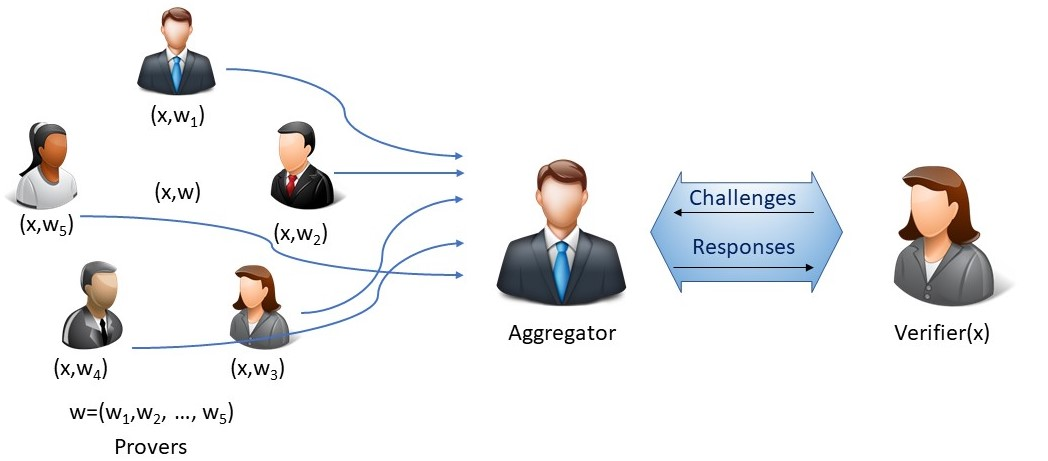
\includegraphics[width=0.9\linewidth]{DPZK.jpg}
%	\caption{Distributed Proof Generation}
%	\label{fig:DPZK}
%\end{figure}

\subsection{Related Notions}
Closely related to our notion is the work of \cite{EfficientTZ} which discusses threshold proofs. This work distributes the prover's side of interactive proofs of knowledge over multiple parties for: (i) improving the security against theft of the user's identity, (ii) improving robustness by ensuring that only a restricted size subset of the provers may be corrupted. The work of \cite{EfficientTZ} primarily captures sigma protocols without allowing interaction among the provers. Our definition captures a broader class of protocols via allowing interaction amongst the provers.  In other words, threshold proofs are a sub-class of the protocols we cater to. Also, other than increasing security via a decentralisation of the prover (or distributing prover's task), our goal is to capture scenarios where multiple provers would like to jointly prove a statement.  Our real-ideal world based definition is inline with MPC style definitions and is more powerful. Pedersen's PhD thesis \cite{Ped92} also defines distributed proofs. Our definition improves the notion of zero-knowledge in \cite{Ped92} where the security model is inherently restricted to a semi-honest collusion of the provers with the verifier. Also, \cite{Ped92} considers the provers' witnesses to always be secret shares of a ``global'' witness and hence the provers' witnesses are \textit{random} when the distributed proof generation begins. But, our definition allows for any distribution on the provers' witnesses, and this impacts some of our security proofs.


%We would like to finally point out that at many scenarios  
%In contrast to the definition in section ~\ref{sec:security model}, all the parties except for the verifier, in the execution of the protocol they may deviate arbitrarily, but the verifier is not allowed to deviate from the protocol. The reason behind considering a preposterously looking adversarial model is that we want to design a zkSNARK which is efficient, secure, publicly verifiable and distributed proof generation property. We know from \cite{}, any interactive honest (public coin) verifier can be transformed into Non-interactive zero-knowledge using \textit{Fiat–Shamir heuristic}. Here the verifier can be semi-honest, i.e., verifier will follow the protocol steps and sends all the challenges uniformly at random.
%-Start with corruption model and give a brief reasoning.
%.\pnote{Describe honest verifier}

\begin{comment}
If all the parties in $\Partyset$ are honest, then the protocol should return 1, this property is called \textbf{\textit{completeness}}.

In this setting, we have two types of corruption models, and that depends on which parties are corrupt:

-- Consider $I$, the set of all corrupt parties consists of all the provers in $\Partyset$, i.e., together they do not have a correct witness for $\stmt$, but they try to cheat in such a way so that the verifier outputs 1. What we want from the protocol is that such a scenario can happen with negligible probability. In other word, whenever in the protocol $\verifier$ outputs 1, then there must be a correct witness $\wit$ such that $\prover_i$ has $\wit_i$ for which $\wit = (\wit_1, \ldots, \wit_{\Num})$, with very high probability. This notion is called \textbf{\textit{proof of knowledge}}. 
	\begin{definition}
		Let $\Func_{\DPZK}$ is the functionality which is defined as ~\ref{func:DPZK} and let $\innp{\Pi}{V}$ is a $\DPZK$ $\Num$-party protocol involving $\Partyset$. We say that $\innp{\Pi}{V}$ realizes $\Func_{\DPZK}$ with computational proof of knowledge property if for every $\ppt$ real world adversary $\Adv$, corrupting at most all provers, there exists a $\ppt$ knowledge extractor $\extrac$ such that for every $\stmt \in L$, for which $\verifier$ outputs 1, $\extrac$ can extract a witness $(\wit_1, \ldots, \wit_{\Num})$ for which $\Func_{\DPZK}$ outputs 1.
	\end{definition}    
	
-- Consider $I$ consists of $\verifier$ and $t$ provers. That is, some of the provers may deviate from the protocol to gain additional information about the honest provers' secret; to achieve this, they may take additional help from $\verifier$'s view. We call a protocol $\innp{\Pi}{\verifier}$ has \textbf{\textit{zero knowledge under t-collusion}}($t$-ZKUC) property, if in this corruption model, corrupted provers and verifier whatever they can compute, the same thing can be computed from the functionality output of the functionality. 
	\begin{definition}
		Let $\Func_{\DPZK}$ is the functionality which is defined as ~\ref{func:DPZK} and let $\innp{\Pi}{V}$ is a $\DPZK$ $\Num$-party protocol involving $\Partyset$. We say that $\innp{\Pi}{V}$ realizes $\Func_{\DPZK}$ with computational zero knowledge under $t$-collusion property if for every $\ppt$ real world adversary $\Adv$, corrupting $I$, at most $t$ provers and verifier, then there exists a $\ppt$ simulator $\Sim$ such that for every $\stmt$, and $\{\wit_i : i\in [\Num]\}$, it holds that: 
		$$\Big\{\Ideal_{\Func_{\DPZK}, \Sim(\secparam),I}(\wit_1, \ldots, \wit_{\Num}) \Big\} \stackrel{c}{\approx} \Big\{ \Real_{\innp{\Pi}{\verifier}, \Adv(\secparam, \wit_T),I}(\wit_1, \ldots, \wit_{\Num}) \Big\}. $$
		Where $\wit_T$ is the input of the corrupt parties.
	\end{definition}

Note that if $I$ consists of the only verifier, then the view of the verifier should not reveal any information about neither the witness nor the inputs of the provers. This notion is called \textbf{\textit{zero knowledge}}, which is subsumed by the notion $t$-ZKUC.
\end{comment}


\section{Construction of DPZK}
We will first discuss how the state-of-art single prover zero-knowledge proof protocols can be made to support distributed proof generation.
\dnote{Should I use zkSNARK protocols instead of zero-knowledge proof protocols}
The literature on single prover zero-knowledge proofs with transparent setup has undergone tremendous progress over the last few years in terms of the concrete proof sizes. The literature has also introduced an ``updatable SRS'' setting \cite{sonic, libra, supersonic} to reduce the trust in the trusted setup with reasonable proof sizes (in between the trusted \cite{pinocchio} and the untrusted setup \cite{aurora, bulletproofs}. \cite{Check} 
Table \ref{tab:SPZK} summarizes the state-of-art protocols in each dimension: proof size, prover and verifier complexities.

Among these works, only Bulletproofs \cite{bulletproofs} discuss distributed proof generation. Even in \cite{bulletproofs}, this discussion was limited to range proofs. In this section, we will discuss how we adapt these protocols to support distributed proof generation. %Looking ahead, all these protocols will be expensive in terms of the complexity of the provers. This will lead us to next section, where we will present our DPZK protocol \name{} which performs better than .
%Note that any protocol can be made to support distributed proof generation by compiling the prover algorithm with an MPC protocol. In this section we will identify the steps in these ZK protocols which can be performed over the shares of the protocol and try to minimize the steps which need to be run using an MPC.

\subsection{DPZK-Aurora}


\subsection{DPZK-Spartan}
Spartan \cite{spartan} is a zkSNARK protocol supporting arbitrary circuits with a transparent setup, $O(|C|^{1/c})$ proof size for $c \geq 2$, an amortized sublinear verifier complexity. Spartan has three high level steps:
\begin{enumerate}
\item Construct a low-degree multivariate polynomial $\tilde{G}$ such that circuit satisfiability can be checked by performing a sum-check protocol \cite{sumcheck} over this polynomial.
\item Use the polynomial commitment scheme from \cite{hyrax} to obtain a commitment of this polynomial from the prover. The traditional sum-check protocol involves the prover sending partial evaluations on this polynomial to the verifier, but this would incur a $O(|C|)$ proof size due to the degree and the number of variables in the polynomial. Instead, the Spartan prover proves these evaluations to the verifier using the polynomial commitment scheme to obtain a succinct proof.
\item Further use polynomial commitments to achieve sub-linear verification time amortized over multiple verifications on the same circuit.
\end{enumerate}
Spartan encodes the extended witness vector $w$ as a polynomial $Z(\cdot)$ such that $Z(i)$ provides the value at wire $i$. Let $\tilde{Z}$ be the polynomial extension of $Z$.
The first step, the construction of the polynomial $\tilde{G}$, involves a multiplication of the polynomial $\tilde{Z}$ on some set of $|C|$ variables $u_1$ with itself on a different distinct set of $|C|$ variables $u_2$ ($\tilde{G}$ will be evaluated on random points in the latter steps). This multiplication is the (only) step which will require an MPC protocol to obtain DPZK-Spartan. 

The multilinear extension $\tilde{Z}(\cdot)$ can be obtained by an inner product of the extended witness vector $w$ with a vector of polynomials on the input variables. Hence, to enable the computation of $\tilde{Z}(u_1) \cdot \tilde{Z}(u_2)$, the prover needs to compute the pairwise product of the elements of $w$. In the DPZK setting, with $w$ being additively shared among the provers, $O(|C|^2)$ MPC multiplications have to be run by the provers. 
\dnote{is the above explanation too succinct?}

%------ Do we need Ligero in this section? since Ligero is subsumed by Aurora in all aspects of SPZK---
%\subsection{DPZK-Ligero}
%We discuss this because this serves as the background to our protocol.
%%Discuss the version with proof size depending on and growing with the number of provers. 

\subsection{DPZK-Bulletproofs}
.\dnote{TODO: circuit share complexity for the Bulletproofs protocol for arbitrary arithmetic circuits}
\begin{comment}
We will give two constructions of distributed proof generation for R1CS with zero knowledge property. In the first construction we will start with reducing the proof for single prover R1CS to single prover zero knowledge inner product argument, then we will give a transformation for zero knwoledge inner product argument from single prover to multiple provers, which will directly imply the proof generation system for multiprover R1CS. In the second construction we will  
\end{comment}
Consider the setting of distributed prover, i.e. that witness is distributed among the provers, say N provers together hold the witness. Here we will discuss the distributed prover version of the bulletproofs for R1CS circuits. We will start with describing the distributed prover version of zero knowledge innerproduct, then we will use the protocol to design a protocol for R1CS.

We will start with reducing a R1CS circuit into multiple inner product. Then we will use the zero knowledge inner product to construct the proof of R1CS circuit. Consider that the circuit has $n$ multiplcation gates. corresponding to the $j^{th}$ wire let $x_j, y_j$ and $z_j$ are the left input, right input and output wires respectively. Then the vectors $\bm{x}, \bm{y}, \bm{z}\in \bbF^n$ can be obtained from the extended witness $\bm{w}$, by multiplying public matrices $A, B, C$ which is depended only on the circuit. Therefore we have 
\begin{align*}
A\bm{w}=\bm{x} \cdots (1)\\
B\bm{w}=\bm{y} \cdots (2)\\
C\bm{w}=\bm{z} \cdots (3)
\end{align*}
and $\bm{x}, \bm{y}, \bm{z}$ will satisfy the following eqution: $\bm{x} o \bm{y} =\bm{z} \cdots (4)$ 

For any $\bm{r}\in \bbF^n$, from equation (1), (2), (3) and (4), the following conditions are true:
\begin{align*}
\langle \bm{r}^T \cdot A, \bm{w}\rangle = \langle \bm{r}, \bm{x} \rangle =v_1 \\
\langle \bm{r}^T \cdot B, \bm{w}\rangle = \langle \bm{y}, \bm{r} \rangle =v_2 \\
\langle \bm{r}^T \cdot C, \bm{w}\rangle = \langle \bm{r}, \bm{z} \rangle =v_3 \\
\langle \bm{r} o \bm{x}, \bm{y} \rangle = \langle \bm{r}, \bm{z} \rangle =v_4 \\
\end{align*} 
We have zero knowledge inner product argument protocol for the following instance:\\
$$\{(P,V,\bm{g},\bm{h},g,h);(\bm{a},\bm{b},\sigma,\delta): P=h^{\sigma}\bm{g}^{\bm{a}}\bm{h}^{\bm{b}}, V=h^{\delta}g^{\langle \bm{a},\bm{b}\rangle}\} \cdots (5)$$
where the public part is $\{(P,V,\bm{g},\bm{h},g,h)$ and secret to the prover is $(\bm{a},\bm{b},\sigma,\delta)$.\\
Define: $v=\langle \bm{a},\bm{b}\rangle$\\
%Finally proving the circuit satisfiability for R1CS can be viewed as 
%$$\{(P_1,P_2,P_3,P_4,P_5,P_6,P_7,P_8, V_1,V_2,V_3,V_4,V_5,V_6,V_7,V_8, P_1=)\}$$
So if we apply the above protocol on these 8 inner products that gives a proof of circuit satisfiability of R1CS, for example consider $\langle \bm{r}^T \cdot A, \bm{w}\rangle = v_1$, in this case consider $\bm{a}=\bm{r}^T\cdot A$, $\bm{b}=\bm{w}$ and $v=v_1$, and use the protocol (5) in these setting.\\
\subsubsection{Multiprover version of zero knowledge inner product argument}
Now we will discuss the multiprover version of the zero knowledge inner product proof: where there will an aggregator $\cA$(need not be trusted) who will iinteract with the verifier.\\
Consider $\cP_1,\ldots, \cP_N$ are provers for the inner product statement i.e. $\{(P,V,\bm{g},\bm{h},g,h)\}$ and the corresponding witness is $(\bm{a},\bm{b}, \sigma, \delta)$, where $P= h^{\sigma} \bm{g}^{\bm{a}} \bm{h}^{\bm{b}}$, $V=h^{\delta}g^{v}$. Let party $\cP_i$ has $(\bm{a}_i,\bm{b}_i,\sigma_i,\delta_i)$ such that
\begin{align*}
	\sum\limits_{i=1}^{N}\bm{a}_i=\bm{a},\text{ }
	\sum\limits_{i=1}^{N}\bm{b}_i=\bm{b},\text{ }
	\sum\limits_{i=1}^{N}\sigma_i=\sigma,\text{ }
	\sum\limits_{i=1}^{N}\delta_i=\delta \text{ }\cdots(5)
\end{align*}
\begin{enumerate}
	\item In this step each party chooses their blinding vectors and commits to that vector. $\cP_i$ samples $\bm{s}^i_L, \bm{s}^i_r \leftarrow_\$ \bbZ_p^n$ and $\rho_i\leftarrow \bbZ_p$, then computes $S^i=h^{\rho_i}\bm{g}^{\bm{s}^i_L}\bm{h}^{\bm{s}^i_R}$ and sends $S^i$ to $\cA$.
	\item $\cA$ computes $S = \prod_{i=1}^{N}S^i = h^{\sum_{i=1}^N\rho_i}\bm{g}^{\sum_{i=1}^N\bm{s}_L^i}\bm{h}^{\sum_{i=1}^N\bm{s}^i_R} = h^{\rho}\bm{g}^{\bm{s}_L}\bm{h}^{\bm{s}_R}$, where $\rho = \sum_{i=1}^{N}\rho_i$, $\bm{s}_L =\sum\limits \bm{s}^i_L,  \bm{s}_R=\sum_{i=1}^{N}\bm{s}^i_R$, and $\cA$ sends $S$ to the verifier $\cV$. In this step $\cA$ computes the commitment of the blinding vector, which is sum of all the provers blinding vector.
	\item Prover $\cP_i$ constructs a vector polynomial $l_i(X)=\bm{a}_i + X. \bm{s}^i_L$ and $r_i(X)=\bm{b}_i + X. \bm{s}^i_R$. All the provers involve in an MPC to obtain the shares of the polynomial $T(X)=\langle \sum_{i=1}^N l_i(X),\sum_{i=1}^N r_i(X)\rangle$. Let $\cP_i$ gets the share $T_i(X)$ of $T(X)$, where $T(X)=\sum_{i=1}^{N}T_i(X)$. Let $T_i(X)= t^i_0+t^i_1.X+t^i_2.X^2$, then $\sum_{i=1}^N t^i_0=\langle \bm{a}, \bm{b} \rangle$. Now $\cP_i$ commits to $t^i_j$ using randomness $\tau^i_j$ i.e. $T^i_j=h^{\tau^i_j}g^{t^i_j}$ and sends $T^i_j$ to $\cA$ for $j\in \{1,2\}$.
	\item $\cA$ computes $T_j=\prod_{i=1}^{N} T^i_j$ which gives the commitment of $t_j \forall j\in\{1,2\}$ and sends $T_1,T_2$ to the verifier $\cV$.
	\item $\cV$ samples $x\leftarrow_\$\bbZ^*_p$ and sends it to the aggregator $\cA$.
	\item $\cA$ sends the $x$ to the provers. 
	\item $\cP$ computes $\bm{l}_i=l_i(x), \bm{r}_i=r_i(x)$, $\mu_i= \sigma_i+\rho_i.x$, $\tau^i_x= \delta_i+\tau^i_1.x+\tau^i_2.x^2$ and sends $\bm{l},\bm{r}, \mu_i, \tau^i_x$ to $\cA$.
	\item $\cA$ defines $\bm{l}=\sum_{i=1}^N\bm{l_i}$ and $\bm{r}=\sum_{i=1}^N\bm{r_i}$ and $\hat{t}=\langle \bm{l},\bm{r}\rangle =T(x)$. $\cA$ computes $Q=\bm{g^lh^r}$, $\mu=\sum_{i=1}^N \mu_i$ and $\tau_x= \sum_{i=1}^{N}\tau_x^i$. And finally $\cA$ sends $Q, \mu, \tau_x, \hat{t}$ to $\cV$.
\end{enumerate}
$\cV$ checks: 
\begin{enumerate}
	\item $h^{\tau_x}g^{\hat{t}}=?V\cdot T_1^x\cdot T_2^{x^2}$ to check the correct evaluation of the committed polynomial $T$ at $x$.
	\item $P\cdot S^x =? h^{\mu}\cdot Q$. 
	\item Runs the inner product proof from \cite{Bulletproofs}, which need not be zero knowledge on the input $(Q, \hat{t}, \bm{g}, \bm{h}, g)$ with the aggregator $\cA$.
\end{enumerate}
The verifier $\cV$ accepts the proof if the checks succeed and the inner product argument accepts.

\begin{comment}
\subsubsection{Completeness} Consider the provers are honest i.e. $\cP_1,\ldots, \cP_N$ together hold the witness i.e. equation (5) is true, then the checks succeed. We will see one by one how all the checks succeed.\\
The first check succeeds because:
\begin{align*}
	h^{\tau_x}g^{\hat{t}} &= h^{\delta+\tau_1 x+ \tau_2 x^2}\cdot g^{\langle \bm{a},\bm{b}\rangle + t_1x+t_2x^2}\\
	&= h^{\sum\limits_{i=1}^N(\delta_i+\tau^i_1x+\tau^i_2x^2)}\cdot g^{\sum\limits_{i=1}^N (t^i_0+t^i_1x+t^i_2x^2)}\\
	&= \prod\limits_{i=1}^N h^{\delta_i}.h^{\tau^i_1x}.h^{\tau^i_2x^2}\prod\limits_{i=1}^N g^{t_0}.g^{t^i_1x}.g^{t^i_2x^2}\\
	&= (h^{\delta}\cdot g^{\langle \bm{a},\bm{b}\rangle})\cdot(h^{\tau_1}g^{t_1})^x\cdot(h^{\tau_2}g^{t_2})^{x^2}\\
	&= V\cdot T_1^x \cdot T_2^{x^2}
\end{align*} 
The second check succeeds because:
\begin{align*}
	P\cdot S^x &= h^{\sigma}\bm{g}^{\bm{a}}\bm{h}^{\bm{b}}\cdot (h^{\rho}\bm{g}^{\bm{s}_L}\bm{h}^{\bm{s}_R})^x\\
	&= h
\end{align*}
\subsubsection{Soundness}
\end{comment}
The completeness, soundness and zero knowledge hold and the proof is similar to zero knowledge inner product argument.\\
We can argue the privacy by saying that provers are interacting only to get the shares of $T(X)$ and that is being done using secure MPC, and remaining all the interactions are done with the aggregator $\cA$ only. Who is learning nothing more than whatever $\cV$ learns in zero knowledge inner produt argument. 
$\cA$ has commitments of the shares of $s_L$ and $s_R$, and computes the commitments of $s_L$ and $s_R$, hiding property of the commitment ensures that $\cA$ learns no information about the secrets $s_L, s_R$ as well as their shares.

$\cA$ receives the commitments of the coefficients of the shares of the polynomial $T(X)$, and reconstructs the commitments of the coefficients of $T(X)$, again hiding property of the commitment ensures that $\cA$ learns no information about the polynomial $T(X)$.

In the next step, $\cA$ gets $\hat{l}, \hat{r}, \mu, \tau_x$, which verifier gets in single prover zero knowledge inner product argument, the zero knowledge property of the above ensures that $\hat{l}, \hat{r}, \mu, \tau_x$ is not leaking any information about the secrets.

Therefore A is not learning anything new. Which implies privacy of the provers are preserved.

\subsubsection{optimization}
We can combine the inner product $\langle \bm{r}^T \cdot A, \bm{w}\rangle = \langle \bm{r}, \bm{x} \rangle =v_1$ and $\langle \bm{r}^T \cdot C, \bm{w}\rangle = \langle \bm{r}, \bm{z} \rangle =v_3$ which can be represented as $\langle \bm{r}^T \cdot(\alpha.A+\gamma.C), \bm{w}\rangle = \langle \bm{r}, (\alpha.\bm{x}+\gamma.\bm{z}) \rangle =v_3$ where $\alpha, \gamma$ are randomly chosen by the verifier $\cV$. In the commitment we are considering that if $\langle \bm{a},\bm{b}\rangle= c$ is in the statement of the inner product, then the commitment of $\bm{a}$ and $\bm{b}$ will be of the form $h^{\sigma} \bm{g}^{\bm{a}} \bm{h}^{\bm{b}}$. Note that in the commitment there should not be any known relation between the generators and for the equation $\langle \bm{r} o \bm{x}, \bm{y} \rangle = \langle \bm{r}, \bm{z} \rangle =v_4$ there should not be the known relation between the generator $\bm{g}$ which is used to commit to $\bm{x}$ with the generator which is used to commit to $\bm{y}$, for that reason the commitment for $\bm{y}$ is considered in left in $\langle \bm{y}, \bm{r} \rangle = v_2$. For that reason this inner product we could not batch with the prior inner products. In this case we need to give 6 inner product proofs instead of 8. 
\dnote{To Protik: Rewrite the section below}.
\subsubsection{Alternate proof for R1CS}
In the beginning we just presented the reduction of R1CS satisfiability to 8 innerproduct argument, where each of them are inner products of vectors of size $n$. Another simple way of combining the inner products of vectors of size $n$ into a single inner product of size of $8n$, (for further optimization, this $8n$ can be reduced to $6n$) were given in \cite{Bulletproofs} in their range proofs. 
For each inner product choose a different set of generators $(\bm{g}^{(k)},\bm{h}^{(k)})_{k=1}^{8}$ and define $\bm{g}$ as the interleaved concatenation of all $\bm{g}^{(k)}$ such that $g_i=g_{\lceil \frac{i}{8} \rceil}^{(i \mod 9)}$. Define $\bm{h}$ in the similar way. The private vectors are also combined in the similar way. Therefore the final inner product will look like:
$$\{(P,V,\bm{g},\bm{h},g,h);(\bm{a},\bm{b},\sigma,\delta): P=h^{\sigma}\bm{g}^{\bm{a}}\bm{h}^{\bm{b}}, V=h^{\delta}g^{\langle \bm{a},\bm{b}\rangle}\}$$
where $a_i= a_{\lceil \frac{i}{8} \rceil}^{(i \mod 9)}$ similarly define $\bm{b}$. $\langle\bm{a},\bm{b}\rangle=\sum_{k=1}^{4}2\times v_i$
In this way proof size will be $2\log (8n) + 2$.


\subsection{Summary of existing protocols}
Argue why we need a better a single prover protocol amenable to multiple provers. 
--- Augment Table \ref{tab:SPZK} with the columns needed for multiple provers and use it for the argument--- 
\begin{center}
	\begin{tabular}{ |c|c|c|c|c|c| } 
		\hline
		Protocols & \multicolumn{2}{c|}{Prover's complexity} & Verifier's complexity & Proof size & rounds \\
		\hline
		&computation & communication& & & \\ 
		\hline
		Ligero & $O(n\log n)M$ & &$O(n)M$ & $O(\sqrt{n})$ & 4\\
		\hline
		Bulletproofs & $O(nE+q(n+m)M)$ & & $O(nE+q(n+m)M)$ & $O(\log n)$ & $\log n$  \\
		\hline
		\name2D & $O((n \log ⁡n)M +nE)$& & $O((n M+n^{1-1/c}E) )$& $O(n^{1/c})$ & 5 \\
		\hline
		\name3D & & & & & \\
		\hline
	\end{tabular}
\end{center}
Here $n$ is the size of the circuit and $c$ is a positive integer of our choice. 
In bulletproofs: $q$ is the linear constraint: $q\leq 2n$ and $m$ such that $W_V \in \bbZ_p^{Q×m}$  such that $W_V$ is of rank $m$.




%\section{Setting up \name{}} 
\section{ZK arguments with $O(\circsize^{1/c})$ proof size and sublinear public key operations for verifier}
We will start with the general framework that have been used to construct zero-knowledge arguments for arithmetic circuits and along with this we provide relevant information on the prior art, before we proceed to detail our two protocols.
The starting point of our protocols is the Interactive PCP (IPCP) argument presented in Ligero~\cite{ligero}.
Ligero uses elementary techniques, is concretely
efficient being devoid of public key operations, and achieves an argument
size which is square-root in size $\circsize$ of the arithmetic circuit. Ligero follows the IPCP paradigm
to first commit to the witness as an oracle. The prover messages of size $O(\sqrt{\circsize})$ are then checked by the verifier by making $O(\sqrt{\circsize})$ queries to the witness oracle.

The core technical
contribution of our first protocol \name2D{} is to use homomorphic commitments and inner product arguments to 
further reduce the size of the queries to the witness oracle. The
reduced access to the witness oracle comes with another surprising benefit: the
verifier restricts its computations to those directly relevant to the parts of
witness being revealed. %This allows us to achieve sublinear verification on average. By carefully restricting the sub-protocols using expensive public key operations to asymptotically smaller circuits (much smaller for practically relevant instantiations),
 We keep the number of public key operations for the
verifier to be strictly sublinear.

Given that we require homomorphic commitments to support distributed proof generation,
the benefits of this single prover protocol are pronounced in the DPZK version.
    
\subsection{Arguments for Arithmetic Circuits}
Our protocol natively supports showing the satisfiability of the $\bbF$-arithmetic circuit for a finite field $\bbF$ which
is an %$\npol$
NP-complete language. For ease of presentation, we produce an argument for the statement ``$\exists \wit, \text{ s.t } \C(\wit)=1$'' for an $\bbF$-arithmetic circuit $\C$. This can be easily modified to yield arguments for the more typical %$\npol$ 
NP language $\calL_C = \{\stmt :\exists \wit \text{ s.t. } \C(\stmt,\wit)=1\}$, which we will briefly discuss later. The satisfiability of an arithmetic circuit $\C$ reduces to proving existence of vectors $x,y,z,\extwit$, where $\extwit$ is the extended witness generated from $\C(\stmt,\wit)$ such that:
$z = x \circ y$,
$x = A \extwit$,
$y = B \extwit$,
$z = C \extwit$ and
$P_{add} \extwit = 0$ for public matrices $A,B,C$ and $P_{add}$ (depending on $\C$). Thus, broadly in the IPCP setting we have the following protocol:
\begin{enumerate}
\item {\bf Oracle Setup}: The prover sets up witness oracle for $x,y,z,\extwit$ and provides query access to the verifier. 
\item {\bf Linear Checks}: The verifier runs a subprotocol with the prover to verify the linear constraints $x=A \extwit$, $y=B \extwit$, $z=C \extwit$, $P_{add} \extwit = 0$.
\item {\bf Quadratic Check}: The verifier runs a subprotocol with the prover to verify $z=x\circ y$.
\end{enumerate}


We will now describe \name2D{}. In brief, \name2D{} will make use of homomorphic commitments over the RS-encoded witness encoding.
%We will commit to the vector $\{\hat{f}^x_i(\eta)\}_{i \in [m]}$ using the homomorphic vector commitments. The vectors corresponding to each $\eta$ will be committed separately. Inner product arguments will then be used to remove the linear dependence of the proof size on the parameter $m$. 
And, instead of ``opening'' vectors from these oracles to the verifier, the prover in \name2D{} will provide an inner product argument on the vectors.
Using the inner-product arguments of \cite{InnerProductDLS, bulletproofs}, \name2D{} achieves the proof size of $O(\circsize^{1/c})$ for any $c \geq 2$ with $O(\circsize^{1-1/c})$ public key operations and $O(\circsize)$ overall complexity for the verifier. 
%-----------------------------------------------------------------------------------------------------
\subsection{Encoding}\label{subsec:encode2D} 

%\subsection{Interactive Protocols for RS-code Oracles}
%\subsubsection{Reed Solomon Witness Encoding}
The linear and quadratic constraints discussed above do not naively admit a sublinear query, i.e, the verifier needs to access complete vectors to be convinced with high probability. Error correcting codes have been used to encode the witness in PCP constructions to enable verification with sublinear query. We discuss two such encodings based on Reed-Solomon codes which have been used in recent constructions \cite{ligero, aurora, STARK2019}.
\begin{comment}
To encode a vector $x\in \bbF^\circsize$, one specifies two domains $G,H\subseteq \bbF$. We will call $G$ as {\em interpolation} domain and $H$ as {\em evaluation} domain. The encoding in \cite{aurora} encodes the vector $x$ as a single Reed-Solomon codeword. This is done by first constructing a polynomial $\hat{f}^x$ which interpolates the vector $x$ on $G$, and then computing its evaluations $\langle \hat{f}^x(\eta) \rangle_{\alpha\in H}$ on points in $H$. The sizes of domains $G$ and $H$ need to be $\Omega(\circsize)$ in the above encoding. For a vector $x$, we will use the notation $\hat{f}^x$ to denote the polynomial interpolating $x$ on $G$, and $f^x$ to denote the vector of evaluations of $\hat{f}^x$ on $H$. Thus in the above scheme, $f^x$ is an encoding of the vector $x$.
\dnote{should we replace the notation $\langle \hat{f}^x(\eta) \rangle_{\alpha\in H}$ with $\langle \hat{f}^x(\eta) \rangle_{\eta \in H}$? Isn't $\eta$ the variable?}

An alternative encoding used in \cite{ligero} encodes parts of a vector separately, and thus the encoded vector corresponds to a set of Reed-Solomon codewords, or a single codeword of an Interleaved Reed-Solomon code (see Definition \ref{defn:interleavedcode}). More specifically, one chooses integers $m$ and $\ell$ such that $m\ell \geq \circsize$ and domains $G$ and $H$ of size $\Omega(\ell)$. The vector $x\in \bbF^\circsize$ is written as
$x=(x_1|\cdots|x_m)$ where $x_i\in \bbF^{\ell}$ for all $i\in [m]$. The vector $x$ is encoded as $(f^x_1,\ldots,f^x_m)$ where $f^x_i$ encodes $x_i$ as described before, i.e $f^x_i=\langle \hat{f}^x_i(\eta)\rangle_{\alpha\in H}$ where the polynomial $\hat{f}^x_i$ interpolates the vector $x_i$ on $G$. 
\end{comment}
%----------------------------------------------------------------------------------------------------
%\Encoding
%-----------------------------------
Let $\extwit \in \bbF^{|\C|}$ be the witness vector. Let $m$ and $\ell$ be integers such that $m\ell\geq \circsize$. we choose ordered domains $G=\{\zeta_1,\ldots,\zeta_\ell\}$ and $H=\{\eta_1,\ldots,\eta_n\}$, We will call $G$ as {\em interpolation} domain and $H$ as {\em evaluation} domain. Then write the vectors $\extwit$ as $\extwit = (\extwit_{1},\ldots,\extwit_{m})$ where each $\extwit_{i}\in \bbF^\ell$ for $i \in [m]$. Construct $Q_i(\cdot)$, a polynomial of degree $<k$, by interpolating the vector $\extwit_{i}$ on $G$ and $Q_{i}(\cdot)$ denotes the corresponding evaluation of $Q_{i}$ on $H$. We define the RS-encoded witness $\ewit\in \bbF^{m\times n}$ as $\ewit[i,j]=Q_{i}(\eta_j)$ for $ i\in [m]$ and $j\in [n]$. We now construct a commitment oracle $\comoracle$ from $\ewit$.
%---------------------------------------------------------------------------------------------------
% Oracle from commitment
%-----------------------------------
\subsection{Oracle Construction}\label{subsec: commit2D}
Throughout, we assume $\bbF$ is a prime field. Let $\com$ denote the Pedersen vector commitment scheme over $\bbF^m$ with randomness space as $\bbF$ and commitment space as group $\bbG$ with independent generators $g_1,\ldots,g_m, h$. Define $c_{j} = \com(\ewit[\cdot,j],\delta_{j})$, $j\in [n]$ where the notation $X[\cdot,j]$ denotes the $m$-length vector $(X[1,j],\ldots,X[m,j])$ and $\delta_{j}$ denotes the randomness for computing the commitment $c_{j}$. We define the oracle $\comoracle$ as $\comoracle[j]=c_{j}$. The oracle $\comoracle$ answers queries of the type $Q\subseteq [n]$, responding with elements $\comoracle[j]$ for $j\in Q$.\footnote{Defining the commitment vector as $\comoracle$ might seem superfluous here. But, the usage of $\comoracle$ will play a prominent role in our 3D protocol. We just define the notation here for the uniformity in our descriptions of the 2D and the 3D versions.} 
%---------------------------------------------------------------------------------------------------
\begin{comment} 
\subsubsection{Linear Check}
	Without loss of generality, we will discuss an argument for proving linear constraints of the form $Ax=0$ where $A$ is a public matrix and $x$ is a (secret) vector. The case $Ax=y$ is easily transformed to the required form by defining $A'=[A|-I]$ and $x'=(x,y)$, and running the protocol on $A'$ and $x'$. Assume that $x\in \bbF^\circsize$ and $A\in \bbF^{\circsize\times \circsize}$. To achieve sublinear query complexity, we do two things: (i) we make a high probability reduction to the problem of proving $\innp{r^TA}{x}=0$ where $r\sample \bbF^\circsize$ is sent by the verifier (ii) encode the witness $x$ using Reed-Solomon code as we described earlier.
	
	We first consider the encoding used in \cite{aurora} which encodes $x$ as a single codeword $f^x$. The prover then provides oracle access to $f^x$. Let $\hat{r}\in\bbF[x]$ be the polynomial that interpolates the vector $r^TA$ on $G$. Then the linear check reduces to checking $\sum_{\zeta\in G}\hat{r}(\zeta) \cdot \hat{f}^x(\zeta) = 0$. In \cite{aurora}, the aforementioned identity is checked with query size of $O(\log|H|)$ using specially developed sumcheck protocol for univariate polynomials. The verifier still incurs $O(\circsize)$ work to compute the encoding $\hat{r}$ for the size $\circsize$ vector $r^TA$. 
	
	We now consider the interleaved encoding of the witness. Looking ahead, the interleaved encoding will have a direct impact on the circuit share complexity of the distributed proof generation in \name{}. Here, we write the vector $x\in \bbF^\circsize$ as $x=(x_1|\cdots|x_m)$ where each $x_i\in \bbF^\ell$ for some $m\ell \geq \circsize$, and $x_m$ padded as necessary. For suitable domains $G$ and $H$, we interpolate each chunk of the vector on $G$ 
	separately via polynomials $\hat{f}^x_1,\ldots,\hat{f}^x_m$. Similarly, we write $r^TA=(r_1,\ldots,r_m)$ with $r_i\in \bbF^n$ and construct polynomials $\hat{r}_i$	for $i\in [m]$. The inner product check $\innp{r^TA}{x}=0$ is then equivalent to checking $\sum_{i\in [m]}\sum_{\zeta\in G}\hat{r}_i(\zeta)\hat{f}^x_i(\zeta)=0$. The	latter is checked by the prover sending the polynomial $\hat{p}=\sum_{i\in
	[m]}\hat{r}_i.\hat{f}^x_i$ to the verifier, and verifier checking $\sum_{\zeta\in G}\hat{p}(\zeta)=0$. Choosing $m,\ell\approx O(\circsize^\frac{1}{2})$ this incurs square-root communication from the prover. How can the verifier be sure that $\hat{p}$ was indeed computed correctly from the witness polynomials $\hat{f}^i_x$? As we formally prove in the later sections, this can be accomplished by the verifier querying the polynomial evaluations (oracles) at a constant number of locations, say $\eta_1,\ldots,\eta_q$. The verifier then checks
	that $\hat{p}$ is consistent at the queried locations by verifying $\hat{p}(\eta_j)=\sum_{i\in [m]}\hat{r}_i(\eta_j)\hat{f}^x_i(\eta_j)$ for
	all $j\in [q]$. This incurs a total query complexity of $q.m=O(\circsize^\frac{1}{2})$.	
	From the perspective of verifier's efficiency, it only needs to compute evaluations of polynomials $\hat{r}_i$, $i\in [m]$ for $\eta\in \{\eta_1,\ldots,\eta_q\}$. %%We will show	that this can be done in expected sublinear time, after a one time $O(||A||)$  pre-processing. We will also discuss why a similar pre-processing does not work for the earlier encoding scheme.
\end{comment}
%---------------------------------------------------------------------------------------------------
%Linear check
%---------------------------
\subsection{Linear Check with Commitment Oracle}\label{subsec:lincheck2D}
The linear check $A\wit=b$ can be reduced to checking $\innp{r^TA}{\wit}=r^Tb$, where the verifier samples a random $r\sample \bbF^{m\ell}$ and sends it to the prover. As in \cite{ligero}, the prover and verifer first compute $R=r^TA$, then write $R$ as $(R_{1}|\cdots|R_{m})$ where each $R_i\in \bbF^\ell$. Both the prover and the verifier also compute degree $<\ell$ polynomials $R_{i}$ interpolating the vector $R_{i}$ on $G$. The required check in terms of polynomials can be expressed as:
\begin{equation}\label{eq:lincheck2D}
\sum_{\zeta\in G}\sum_{j\in [m]}
R_{i}(\zeta) \cdot Q_{i}(\zeta) = r^Tb.
\end{equation}
The prover computes the polynomial $p(\cdot)=\sum_{i\in[m]}R_i(\cdot) \cdot Q_i(\cdot)$. This polynomial $p(\cdot)$ of degree $< k+\ell-1$ is sent to the verifier who checks $\sum_{\zeta\in G}p(\zeta)=r^Tb$. The verifier needs to check if the polynomial $p(\cdot)$ is correctly computed from the witness oracle $\comoracle$ to guard against dishonest provers. Following \cite{ligero}, it is enough for the verifier to query the polynomial evaluations at a constant number of locations, say $\eta_{j_1},\ldots,\eta_{j_u}$ and then check that $p(\cdot)$ is consistent at the queried locations. We observe that the verifier only uses these queried values to prove some inner-product relations with other (publicly-known) vectors. Hence, our idea is to make the prover use inner-product arguments to prove the consistency of $p(\cdot)$ to the verifier.

We will now formally describe the linear check for our protocol \name2D{}. It will check that a purported commitment oracle $\comoracle$ encodes witness $\wit$ satisfying the constraint $A\wit=b$ for a public matrix $A$ and $b$ is a public vector. As before, we assume $\wit \in \bbF^{\circsize}$ and $A\in \bbF^{\circsize\times \circsize}$ and
$\circsize = m \ell$ for some positive integers $m$ and $\ell$. We further assume that the prover has RS-encoded oracle $\ewit$ which opens to the commitment $\comoracle$ and is $e$-close to the interleaved code $L^{m}$. The prover and the verifier interact as follows: 

%$\prover$ sets $\cm_x$ as the oracle.
\begin{figure}[h!]
	\centering
	\begin{framed}
		\begin{itemize}
			\item {$\linearcheckTwoD (\FF, \GG, L[n,k,d], m, t, A \in \FF^{m\ell \times m\ell}, b\in \FF^{m\ell}, \bm{g}, [\pi]; \wit)$}:
			
			\item {\bf Relation}: $\exists \wit, \ewit$ s.t. $\ewit = \open(\pi), \ewit = \enc(\wit)$ and $A\wit = b$. 
			
			\item {\bf Oracle Setup}: The prover $\prover$ computes $\ewit = \enc(\wit)$ and $\comoracle = \com(\ewit)$ as in Sections ~\ref{subsec:encode2D} and ~\ref{subsec: commit2D}. The prover sets $\pi := \comoracle$ as the oracle.
		\end{itemize}
		\begin{enumerate}[{\rm 1.}]
			\item $\verifier \rightarrow \prover: $ $\verifier$ picks a random $r\in \bbF^{ml}$ and sends that $r$ to $\prover$.
			
			\item Both $\prover$ and $\verifier$ compute $R=r^TA$, which is a vector of size $m\ell$. Read $R$ in a matrix form where first $l$ elements of $R$ form the first row, next $l$ elements form the second row, similarly $R$ will have $m$ rows. Then they construct polynomials $R_i(\cdot)$ of degree $<l$ such that $R_i(\zeta_j)=R_{ij}$ $\forall i\in [m], j\in [\ell]$. 
			
			\item $\prover \rightarrow \verifier: $  $\prover$ computes a polynomial $p(\cdot)=\sum_{i\in[m]} ( R_i(\cdot)\cdot \hat{f}^x_i(\cdot))$ and sends $p(\cdot)$ to $\verifier$.
			
			\item $\verifier \rightarrow \prover: $ $\verifier$ samples $t$ distinct  indices $j_1,\ldots,j_t$ from the set $[n]$ independently at random and sends the indices to $\prover$.
			
			\item Oracle Queries: $\verifier$ queries the oracle $\pi$ with $\{j_u : u\in [t]\}$.
			
			\item Oracle Answers: The oracle replies with $\pi[j_u], u\in [t]$.
			
			\item $\prover \leftrightarrow \verifier: $ $\prover$ and $\verifier$ run a inner product subprotocol for each $u\in[t]$:
			\begin{itemize}
				\item $\innerproduct(\GG,\bm{g}, R_{j_u}, \pi[j_u], p(\eta_{j_u}); \ewit[\cdot,j_u])$ $\forall u\in [t]$,
				
				Where $R_{j_u} = (R_1( \eta_{j_u}) , \ldots , R_m( \eta_{j_u}))$ and $\ewit[\cdot,j_u]$ denotes the $m$-length vector $(\ewit[1,j_u], \ldots, \ewit[m,j_u])$ and $\pi[j_u] = \com(\ewit[\cdot, j_u])$. $\verifier$ proceeds if the arguments succeed for all $u \in [t]$.
			\end{itemize} 
			
			\item $\verifier$ also checks that $\sum_{j\in[l]} p(\zeta_j)=0$.
			
			\item $\verifier$ accepts if all the above checks are succeed.	  
		\end{enumerate}
	\end{framed}
	\caption{Linear Check for $\name$2D}
\end{figure}
The correctness of the above protocol follows from the correctness of \cite{ligero} and the inner product argument. We now prove the proof of knowledge of the protocol through the following lemma.
\begin{lemma}
	For a $P^*$ which makes a verifier accept the above linear check protocol, there is an expected $\ppt$ extractor $\extr$ with rewinding access to $P^*$ which outputs a valid witness or breaks the binding of the commitment scheme with overwhelming probability.
\end{lemma}
.\dnote{We should probably include a defn of proof of knowledge in the prelims. Even if we extend this lemma to witness extended emulation, we do not have a single prover definition for WEE in the paper.}
\begin{proof}
	Let $\extr_{\ip}$ be the $\ppt$ extractor for the inner product argument used. For a transcript, the prover's messages include the polynomial $p(\cdot)$ and its messages during the inner-product argument of $\innp{R_{j_u}}{\ewit[\cdot,j_u]} = p(\eta_{j_u})$.
	$\extr$ would use $\extr_\ip$ with the commitment $\comoracle[j_u]$ to obtain $\ewit[\cdot,j_u]$ in expected polynomial time. 
	
	To obtain a valid witness for the linear check protocol, $\extr$ rewinds the prover to Step 4 after obtaining an accepting transcript. $\extr$ adds the set of $j_u$ indices obtained to a set $S$ and repeats the rewinding process till $|S| = n$. 
	There are two possibilities here for the obtained matrix $U$:
	\begin{itemize}
		\item if $d(U, L^m) > e$, $\extr$ outputs $U$. (The proximity check would have verified $d(U,L^m) \leq e$, and hence a $U$ otherwise would mean $\extr$ outputs a collision to the commitment scheme used).
		\dnote{should we define a valid witness as one with distance less than $e$? Else, it seems like we can't have an independent proof and we have to bring in proximity check verifying $d<e$.}
		\item if $d(U, L^m) \leq e$, the soundness analysis for the linear check in \cite{ligero} ensures that $U$ decodes to $x$ such that $A\wit=b$ with overwhelming probability. %and hence $\com(\calU^*)=\cm$.
	\end{itemize}
	An analysis similar to the one in the proof of Lemma~\ref{lem:proximity} proves that $\extr$ can attain $|S| = n$ in an expected polynomial time.
\end{proof}
%-------------------------------------------------------------------------------------------------
\begin{comment}
\subsubsection{Quadratic Check}
The quadratic check involves the prover convincing the verifier that $x\circ y=z$ by providing oracle access to the vectors $x,y$ and $z$. Again, we
consider the encoding by parts we discussed for the linear check. We write $x=(x_1|\cdots|x_m)$, $y=(y_1|\cdots|y_m)$ and $z=(z_1|\cdots|z_m)$ and
construct polynomials $\hat{f}^x_i$, $\hat{f}^y_i$ and $\hat{f}^z_i$ for $i\in [m]$ as before. The quadratic check then reduces to showing that
$\hat{f}^x_i(\zeta) \cdot \hat{f}^y_i(\zeta)-\hat{f}^z_i(\zeta)=0$ for all $i\in [m]$ and $\zeta\in G$. With high probability, the above can be checked by
verifier sending a random vector $r\sample \bbF^m$ to the prover, and prover sending the polynomial $\hat{p}=\sum_{i\in [m] } r_i (\hat{f}^x_i \cdot \hat{f}^y_i - \hat{f}^z_i)$ to the verifier. The verifier checks that $\hat{p}(\zeta)=0$ for all $\zeta\in G$. The verifier also checks that $\hat{p}$ is correctly computed from the oracles by querying the oracles at small number of points $\eta_1,\ldots,\eta_q$ and checking that $\hat{p}(\eta_j)=\sum_{i\in [m]}r_i(\hat{f}^x_i(\eta_j)\cdot\hat{f}^y_i(\eta_j)-\hat{f}^z_i(\eta_j))$ for $j\in [q]$.
\end{comment}
%----------------------------------------------------------------------------------------------------
%Quadratic check
%---------------------------------
\subsection{Quadratic Check}\label{subsec:quadcheck2D}
We now formally describe the interactive oracle protocol for checking the relation $x\circ y = z$ for vectors $x,y,z\in \bbF^\circsize$. Let $\ewit_x, \ewit_y$ and $\ewit_z$ denote the encodings of vectors $x$, $y$ and $z$ respectively via the RS code mentioned in Section ~\ref{subsec:encode2D}. Let $\comoracle_x,\comoracle_y$ and $\comoracle_z$ denote the respective commitment oracles. In brief, as in the linear check, it follows \cite{ligero} except to check whether $p(\cdot)$ is correctly computed from the oracles. When the verifier queries the oracles at small number of points $\eta_{j_1} , \ldots , \eta_{j_t}$, the prover and the verifier would involve in an inner-product argument for the verifier to verify that $p(\eta_{j_u})=\sum_{i\in [m]}r_i[Q^x_i(\eta_{j_u}) \cdot Q^y_i(\eta_{j_u})-Q^z_i(\eta_{j_u}))$ for $u\in [t]$.
Which can be viewed as:
\begin{align*}
&\innp{r}{(\ewit_x[\cdot,j_u]\cdot \ewit_y[\cdot,j_u] - \ewit_z[\cdot,j_u])} = p(\eta_{j_u}) \\
\Rightarrow &\innp{r}{(\ewit_x[\cdot,j_u]\cdot \ewit_y[\cdot,j_u])} + \innp{r}{-\ewit_z[\cdot,j_u]} = p(\eta_{j_u})
\end{align*}
%------------------------------------------------------------------------
There are two inner products in the above statement and the prover does not want to reveal the values of the individual inner products. Hence, \name2D combine them into a single inner product relation.

For each $u\in[t]$, $\prover$ runs the following inner product arguement with $\verifier$:
$$\innp{(r\circ \ewit_x[\cdot,j_u]||r)}{(\ewit_y[\cdot,j_u]||-\ewit_z[\cdot,j_u])} = p(\eta_{j_u})$$
To facilitate this, $\ewit_x, \ewit_y$ and $\ewit_z$ should have been committed with different independently chosen sets of generators. And, the set of generators used for committing $r$ (to be concatenated with $r \circ \ewit_x [\cdot, j_u])$ should also be independent of the above three sets of generators. $\verifier$ proceeds if the arguements succeed for all $u\in[t]$.
%-----------------------------------------------------------------------

%	$\prover$ sets $\cm_x, \cm_y$ and $\cm_z$ as the oracles.
\begin{figure}[h!]
	\centering
	\begin{framed}
		\begin{itemize}
			\item {$\quadcheckTwoD (\FF, \GG, L[n,k,d], m, t, \bm{g}_x, \bm{g}_y, \bm{g}_z, [\pi]; \wit_x, \wit_y, \wit_z)$}:
			\item {\bf Relation}: $\exists (\wit_x, \wit_y, \wit_z, \ewit_x, \ewit_y, \ewit_z)$ such that $(\ewit_x, \ewit_y, \ewit_z) = \open(\pi)$ and $\ewit_a = \enc(\wit_a)$ for $a\in \{x,y,z\}$ and $\wit_x \circ \wit_y = \wit_z$.
			\item {\bf Oracle Setup}: The prover $\prover$ computes $\ewit_a = \enc(\wit_a)$ and $\comoracle_a = \com(\ewit_a)$ for $a\in \{x,y,z\}$. It sets $\pi := [\comoracle_{x} || \comoracle_{y} || \comoracle_{z}]$ where the notation denotes vertical stacking of the vectors. Note that the generators used to construct commitment vectors for $\wit_x, \wit_y$ and $\wit_z$ should be independent. So, $\prover$ and $\verifier$ together generates $\bm{g}_x$, $\bm{g}_y$ and $\bm{g}_z$.
		\end{itemize}
		\begin{enumerate}
			\item $\verifier \rightarrow \prover: $ $\verifier$ picks $r$ uniformly at random from $\FF^{m}$ and sends it to $\prover$.
			
			\item $\prover \rightarrow \verifier: $ $\prover$ computes the polynomial $p(\cdot)= \sum_{i\in [m]} [r_i\cdot (Q^x_i(\cdot)\cdot Q^y_i(\cdot) - Q^z_i(\cdot))] $ and sends $p(\cdot)$ to $\verifier$. 
			
			\item $\verifier \rightarrow \prover: $ $\verifier$ sends $t$ randomly sampled indices $Q=\{j_u\}_{u\in[t]}$ from $[n]$.
			
			\item Oracle Queries: $\verifier$ queries the oracle $\pi$ with $\{j_u : u\in [t]\}$.
			\item Oracle Answers: The oracle responds with $\pi[j_u], u\in[t]$.
			\item $\prover \leftrightarrow \verifier: $ $\prover$ and $\verifier$ together generates $\bm{g}$ independent of all the generators used in committing $x,y,z$. Both run a inner product subprotocol for each $u\in[t]$:
			\begin{itemize}
				\item $\innerproduct(\GG,\bm{g}'||\bm{g}_r, \bm{g}_y||(\bm{g}_z)^{-1}, \comoracle_x[j_u]\cdot (\bm{g}_r)^r, p(\eta_{j_u}), \comoracle_y\cdot (\comoracle_z)^{-1}; r\circ\ewit_x[\cdot,j_u]||r, \ewit_y[\cdot,j_u]||-\ewit_z[\cdot,j_u])$ $\forall u\in [t]$,
				
				Where $\bm{g}'= (g'_1, \ldots, g'_m)$ is such that $g'_i = g_x^{r^{-1}}$ 
				$\verifier$ proceeds if the arguments succeed for all $u \in [t]$.
			\end{itemize} 
			%.\pnote{run a subprotocol to prove the innerproduct arguement for the following statement $\innp{r\circ \ewit_x[\cdot,j_u]}{\ewit_y[\cdot,j_u]} - \innp{r}{\ewit_z[\cdot,j_u]} = p(\eta_{j_u})$ $\forall u\in[t]$.} 
			
			\item $\verifier$ checks if $p(\zeta_j)=0$ $\forall j\in[l]$. If yes then accepts, else rejects.
		\end{enumerate}
	\end{framed}
	\caption{Quadratic Check for $\name$2D}
\end{figure}

%----------------------------------------------------------------------------------------------------------------------------
\begin{comment}
\begin{figure}[h!]
\centering
\begin{framed}
\begin{itemize}
\item {$\quadcheckTwoD (\FF, \GG, L, [\pi]; \wit_x, \wit_y, \wit_z)$}:
\item {\bf Relation}: $\exists (\wit_x, \wit_y, \wit_z, \ewit_x, \ewit_y, \ewit_z)$ such that $(\ewit_x, \ewit_y, \ewit_z) = \open(\pi)$ and $\ewit_a = \enc(\wit_a)$ for $a\in \{x,y,z\}$ and $\wit_x \circ \wit_y = \wit_z$.
\item {\bf Oracle Setup}: The prover $\prover$ computes $\ewit_a = \enc(\wit_a)$ and $\comoracle_{xy} = \com(\ewit_x \circ \ewit_y)$, $\comoracle_z = \com(\ewit_z)$. It sets $\pi :=[\comoracle_{xy} || \comoracle_{z}]$ where the notation denotes vertical stacking of the vectors that means $\pi$ has $n$ columns and 2 rows such that $\pi[1,j] = \comoracle_{xy}[j]$ and $\pi[2,j] = \comoracle_{z}[j]$ $\forall j\in[n]$.
\end{itemize}
\begin{enumerate}
\item $\verifier \rightarrow \prover: $ $\verifier$ picks $r$ uniformly at random from $\FF^{m}$ and sends it to $\prover$.

\item $\prover \rightarrow \verifier: $ $\prover$ computes the polynomial $p(\cdot)= \sum_{i\in [m]} [r_i\cdot (\hat{f}^x_i(\cdot)\cdot \hat{f}^y_i(\cdot) - \hat{f}^z_i(\cdot))] $ and sends $p(\cdot)$ to $\verifier$. 

\item $\verifier \rightarrow \prover: $ $\verifier$ sends $t$ randomly sampled indices $Q=\{j_u\}_{u\in[t]}$ from $[n]$.

\item Oracle Queries: $\verifier$ queries the oracle $\pi$ with $\{j_u : u\in [t]\}$.
\item Oracle Answers: The oracle responds with $\pi[j_u], u\in[t]$.
\item $\prover \leftrightarrow \verifier: $ $\prover$ and $\verifier$ run a inner product subprotocol for each $u\in[t]$:
\begin{itemize}
\item $\innerproduct(\GG,\bm{g}, r, \pi[1,j_u]\cdot \pi[2,j_u]^{-1}, p(\eta_{j_u}); \ewit_x[\cdot,j_u] \circ \ewit_y[\cdot, j_u], \ewit_z[\cdot,j_u])$ $\forall u\in [t]$,
%Where $R_{j_u} = (R_1( \eta_{j_u}) , \ldots , R_m( \eta_{j_u}))$ and $\ewit[\cdot,j_u]$ denotes the $m$-length vector $(\ewit[1,j_u], \ldots, \ewit[m,j_u])$ and $\pi[j_u] = \com(\ewit[\cdot, j_u])$.

$\verifier$ proceeds if the arguments succeed for all $u \in [t]$.
\end{itemize} 
\begin{comment}
.\pnote{run a subprotocol to prove the innerproduct arguement for the following statement $\innp{r\circ \ewit_x[\cdot,j_u]}{\ewit_y[\cdot,j_u]} - \innp{r}{\ewit_z[\cdot,j_u]} = p(\eta_{j_u})$ $\forall u\in[t]$.} 

There are two inner products in the above statement and the prover does not want to reveal the values of the individual inner products. Hence, \name2D combine them into a single inner product relation.

For each $u\in[t]$, $\prover$ runs the following inner product arguement with $\verifier$:
$$\innp{(r\circ \ewit_x[\cdot,j_u]||r)}{(\ewit_y[\cdot,j_u]||-\ewit_z[\cdot,j_u])} = p(\eta_{j_u})$$
To facilitate this, $\ewit_x, \ewit_y$ and $\ewit_z$ should have been committed with different independently chosen sets of generators. And, the set of generators used for committing $r$ (to be concatenated with $r \circ \ewit_x [\cdot, j_u])$ should also be independent of the above three sets of generators. $\verifier$ proceeds if the arguements succeed for all $u\in[t]$.

\item $\verifier$ checks if $p(\zeta_j)=0$ $\forall j\in[l]$. If yes then accepts, else rejects.
\end{enumerate}
\end{framed}
\caption{Quadratic Check for $\name$2D}
\end{figure}
\end{comment}
%----------------------------------------------------------------------------------------------------------------------------

The correctness of the above protocol again follows from the correctness of \cite{ligero} and the inner product argument. Its proof of knowledge property is proved through the following lemma.
\begin{lemma}
	For a $P^*$ which makes a verifier accept the quadratic check protocol, there is an expected $\ppt$ extractor $\extr$ with rewinding access to $P^*$ which outputs valid witnesses $\ewit_x$, $\ewit_y$ and $\ewit_z$ with overwhelming probability.
\end{lemma}
\begin{proof}
	Let $\extr_{\ip}$ be the $\ppt$ extractor for the inner product argument used. For a transcript, the prover's messages include the polynomial $p(\cdot)$ and its messages during the inner-product argument.
	$\extr$ would use $\extr_\ip$ to obtain $\left( (r \circ \ewit_x[\cdot,j_u] \, || \, r \right)$ and $\left( \ewit_y[\cdot,j_u] \, || \, -\ewit_z[\cdot,j_u] \right)$ in expected polynomial time. $\extr_\ip$ would use the commitments derived from $\comoracle_x[j_u]$, $\comoracle_y[j_u]$ and $\comoracle_z[j_u]$. From this output of $\extr_{\ip}$, $\extr$ can obtain $\ewit_x[\cdot,j_u]$, $\ewit_y[\cdot,j_u]$ and $\ewit_z[\cdot,j_u]$.
	
	To obtain a set of valid witnesses for the quadratic check protocol, $\extr$ rewinds the prover to Step 3 after obtaining an accepting transcript. $\extr$ adds the set of $j_u$ indices obtained to a set $S$ and repeats the rewinding process till $|S| = n$. At this point, $\extr$ has the complete $\ewit_x$, $\ewit_y$ and $\ewit_z$. There are two possibilities here:
	\begin{itemize}
		\item if $d(\ewit_\delta,L^m) > e$ for each $\delta = \{x, y, z\}$, $\extr$ outputs $\ewit_\delta$. (The proximity check would have verified $d(\ewit,L^m) \leq e$, and hence a $\ewit$ otherwise would mean $\extr$ outputs a collision to the commitment scheme used).
		\item if $d(\ewit_\delta,L^m) \leq e$ for each $\delta = \{x, y, z\}$, the soundness analysis for the quadratic check in \cite{ligero} ensures that $\ewit_\delta$ decodes to $\delta$ such that $x\circ y = z$ with overwhelming probability.
	\end{itemize}
	An analysis similar to the one in the proof of Lemma~\ref{lem:proximity} proves that $\extr$ can attain $|S| = n$ in an expected polynomial time.
\end{proof}
%---------------------------------------------------------------------------------------------------
\begin{comment}
\subsubsection{Proximity Test}
The correctness of the previous two checks, namely the linear check and the
quadratic check rely on the fact that the witness oracles are evaluations of
``low'' degree polynomials. There are several known low degree tests for polynomials
from PCP literature. The protocol in \cite{aurora} uses a recent test for
proximity by Ben-Sasson et al.\cite{IOPP_FRI2018} with particularly efficient
prover and $O(\log d)$ query complexity for polynomials of degree at most $d$. 
We use a variant of proximity test from \cite{ligero}, adapting it to work
with homomorphic commitments of the RS-encoded oracles and reducing the query
complexity.
\end{comment}
%---------------------------------------------------------------------------------------------------
%Proximity Check
%-----------------------------
\subsection{Proximity Protocol}\label{subsec:proximity2D}
The correctness of the previous two checks, namely the linear check and the
quadratic check rely on the fact that the witness oracles are evaluations of
``low'' degree polynomials. There are several known low degree tests for polynomials
from PCP literature. The protocol in \cite{aurora} uses a recent test for
proximity by Ben-Sasson et al.\cite{IOPP_FRI2018} with particularly efficient
prover and $O(\log d)$ query complexity for polynomials of degree at most $d$. 
We use a variant of proximity test from \cite{ligero}, adapting it to work
with homomorphic commitments of the RS-encoded oracles and reducing the query
complexity.

We finally describe our protocol for ``proximity'' of a purported codeword to the interleaved code. Let $U\in \bbF^{m\times n}$ denote the purported codeword and let $e< d/3$ denote the proximity parameter. The commitment oracle $\comoracle$ corresponds to $U$.
\dnote{To Nitin: why did you not use the notation $\rsoracle$ for $U$? Is it that only those $U$s which satisfy the proximity test become $\rsoracle$?}
The prover and the verifier interact as follows:
%$\prover$ sets $\cm$ as the oracle.
\begin{figure}[h!]
	\centering
	\begin{framed}
		\begin{itemize}
			\item {$\proxcheckTwoD(\FF, \GG, L[n,k,d], m, t, \bm{g}, [\pi]; \ewit)$}:
			\item {\bf Relation}: $\ewit = \open(\pi)$, $\ewit \in L^m$.
			\item {\bf Oracle Setup}: Prover computes $\comoracle$ from $\ewit$ as in Section ~\ref{subsec: commit2D} and sets $\pi := \comoracle$ as the oracle.
		\end{itemize}
		\begin{enumerate}
			\item $\verifier \rightarrow \prover :$ $\verifier$ as a challenge picks $\gamma \in \bbF^m$ uniformly at random and sends it to $\prover$.
			
			\item $\prover \rightarrow \verifier :$ $\prover$ computes $\w=\gamma^T\ewit$ and sends $\w$ to $\verifier$.
			
			\item $\verifier \rightarrow \prover :$ $\verifier$ picks a random subset $Q\subseteq [n]$ such that $|Q|=t$ and sends $Q$ to $\prover$.
			
			\item Oracle Queries: $\verifier$ queries the oracle $\pi$ with $\{j_u:u\in[t]\}$.
			
			\item Oracle Answers: The oracle responds with $\pi[j_u], u\in[t]$.
			
			\item $\prover \leftrightarrow \verifier: $ $\prover$ and $\verifier$ run a inner product subprotocol for each $u\in[t]$:
			\begin{itemize}
				\item $\innerproduct(\GG, \bm{g}, \gamma, \pi[j_u], \w_{j_u}; \ewit[\cdot,j_u])$ $\forall u\in [t]$.
			\end{itemize}
			%run a subprotocol to prove the innerproduct arguement for the following statement $\innp{\gamma}{\ewit_x[\cdot,j_u]}=u_{j_u}$ $\forall j_u\in Q$
			
			\item If $\verifier$ accepts the innerproduct arguement in the previous step, then checks if $\w\in L$. If yes then $\verifier$ outputs accept else outputs reject.
		\end{enumerate}
	\end{framed}
	\caption{Proximity Check for $\name$2D}
\end{figure}
The correctness of the above protocol follows from \cite{ligero} and the inner product argument. The following lemma captures its proof of knowledge property.
\begin{lemma}\label{lem:proximity}
	For a $P^*$ which makes a verifier accept the proximity protocol, there is an expected $\ppt$ extractor $\extr$ with rewinding access to $P^*$ which outputs a valid witness or breaks the binding of the commitment scheme with overwhelming probability.
\end{lemma}
\begin{proof}
	Let $\extr_{\ip}$ be the $\ppt$ extractor for the inner product argument used. For a transcript, the prover's messages include the polynomial $p$ and its messages during the inner-product argument of $\innp{\gamma}{U[\cdot, j_u]} = w_{j_u}$.
	$\extr$ would use $\extr_\ip$ with the commitment $\comoracle[j_u]$ to obtain $U[\cdot,j_u]$ in expected polynomial time. 
	
	To obtain a valid witness for the proximity protocol, $\extr$ rewinds the prover to Step 3 after obtaining an accepting transcript. $\extr$ adds the set of $j_u$ indices obtained to a set $S$ and repeats the rewinding process till $|S| = n$. Let the obtained matrix be $U$.
	The soundness analysis for the proximity check in \cite{ligero} ensures that  $d(U, L^m) \leq e$ with overwhelming probability. 
	
	We will now estimate the number of rewindings required for $\extr$ to reach $|S| = n$. We will provide a crude upper bound on this to show that $\extr$ runs in expected polynomial time. To start with, we consider $t=1$. A larger $t$ will only reduce the number of rewindings required. Let $X_i$ be the discrete random variable that represents the number of rewindings to improve from $|S| = i-1$ to $|S| = i$ i.e., to pick a column not in $S$ when $|S| = i-1$. The base case $X_1=1$ because the first column selected will always be distinct. When $|S| = i-1$, there are $n-i+1$ columns remaining, the probability of selecting one of them is $(n-i+1)/n$. Since $X_i$ follows the geometric distribution, 
	\[
	E[X_i] = 1/ [(n-i+1)/n] = n/ (n-i+1)
	\]
	Let $X$ be the random variable for the number of rewindings to reach $|S| = n$.
	Following linearity of expectations, 
	\[
	E[X] = \sum_{i \in [n]} E[X_i] = \sum_{i \in [n]} n/ (n-i+1) = n \sum_{i \in [n]} 1/i = \theta (n \log n) 
	\]
	Thus, $\extr$ extracts the witness in an expected polynomial time.
\end{proof}
%--------------------------------------------------------------------------------------------------
\begin{comment} 
\section{\name2D{} - ZK arguments with $O(\circsize^{1/c})$ proof size and sublinear public key operations for verifier}
We will now describe \name2D{}. In brief, \name2D{} will make use of homomorphic commitments over the RS-encoded witness oracles.
%We will commit to the vector $\{\hat{f}^x_i(\eta)\}_{i \in [m]}$ using the homomorphic vector commitments. The vectors corresponding to each $\eta$ will be committed separately. Inner product arguments will then be used to remove the linear dependence of the proof size on the parameter $m$. 
And, instead of ``opening'' vectors from these oracles to the verifier, the prover in \name2D{} will provide an inner product argument on the vectors.
Using the inner-product arguments of \cite{InnerProductDLS, bulletproofs}, \name2D{} achieves the proof size of $O(\circsize^{1/c})$ for any $c \geq 2$ with $O(\circsize^{1-1/c})$ public key operations and $O(\circsize)$ overall complexity for the verifier. 

\subsection{Encoding}\label{subsec:encode2D} 
Let $\extwit \in \bbF^{|\C|}$ be the witness vector. Let $m$ and $\ell$ be integers such that $m\ell\geq \circsize$. We choose ordered domains $G=\{\zeta_1,\ldots,\zeta_\ell\}$ and $H=\{\eta_1,\ldots,\eta_n\}$. We then write the vectors $\extwit$ as $\extwit = (\extwit_{1},\ldots,\extwit_{m})$ where each $\extwit_{i}\in \bbF^\ell$ for $i \in [m]$. Construct $Q_i(\cdot)$, a polynomial of degree $<k$, by interpolating the vector $\extwit_{i}$ on $G$ and $Q_{i}$ denotes the corresponding evaluation of $Q_{i}$ on $H$. We define the RS-encoded witness $\ewit\in \bbF^{m\times n}$ as $\ewit[i,j]=Q_{i}(\eta_j)$ for $ i\in [m]$ and $j\in [n]$. We now construct a commitment oracle $\comoracle$ from $\ewit$.
\dnote{do we use the notation $f^x_i$?}
%If $|x|=ml$ then read $x$ as 
%$$x=
%\begin{bmatrix}
%x_{11} & x_{12} & \ldots & x_{1l}\\
%x_{21} & x_{22} & \ldots & x_{2l}\\
%& \vdots\\
%x_{m1} & x_{m2} & \ldots & x_{ml}
%\end{bmatrix}
%$$	
%Construct polynomials $\hat{f}^x_i(\cdot)$ of deg $k$ such that $\hat{f}^x_i(\zeta_j)=x_{ij}$ $\forall i\in [m], j\in [l]$ where $k>l$ and $l+t=k$.
%
%Define 
%$$ \ewit =
%\begin{bmatrix}
%u_{11} & u_{12} & \ldots & u_{1n}\\
%u_{21} & u_{22} & \ldots & u_{2n}\\
%& \vdots\\
%u_{m1} & u_{m2} & \ldots & u_{mn}
%\end{bmatrix}
%$$
%where $u_{ij}= \hat{f}^x_i(\eta_j)$ $\forall i\in[m], j\in[n]$ $n>k$. $\bm{\zeta}=\{\zeta_1,\ldots,\zeta_l\}$ we will call it interpolation domain and $\bm{\eta} = \{\eta_1,\ldots,\eta_n\}$ we will call it evaluation domain. 
%
%Let $L$ be the set of codewords and the above linear code has distance $d$. Then a correctly computed $\ewit_x$ is in $L^m$.
 
\subsection{Oracle Construction}\label{subsec: commit2D}
Throughout, we assume $\bbF$ is a prime field. Let $\com$ denote the Pedersen vector commitment scheme over $\bbF^m$ with randomness space as $\bbF$ and commitment space as group $\bbG$ with independent generators $g_1,\ldots,g_m, h$. Define $c_{j} = \com(\ewit[\cdot,j],\delta_{j})$, $j\in [n]$ where the notation $X[\cdot,j]$ denotes the $m$-length vector $(X[1,j],\ldots,X[m,j])$ and $\delta_{j}$ denotes the randomness for computing the commitment $c_{j}$. We define the oracle $\comoracle$ as $\comoracle[j]=c_{j}$. The oracle $\comoracle$ answers queries of the type $Q\subseteq [n]$, responding with elements $\comoracle[j]$ for $j\in Q$.\footnote{Defining the commitment vector as $\comoracle$ might seem superfluous here. But, the usage of $\comoracle$ will play a prominent role in our 3D protocol. We just define the notation here for the uniformity in our descriptions of the 2D and the 3D versions.} 
%We will use $\comoracle$ as the witness
%oracle, and adapt the subprotocols for checking linear constraints, quadratic
%constraints and proximity to this oracle.

%Let $\cm_x=(c_1,\ldots c_n)$ where 
%$c_j= \com( \begin{bmatrix}
%u_{1j} & u_{2j} & \ldots & u_{mj}
%\end{bmatrix}^T)$ $\forall j\in [n]=\comoracle_x$

\begin{comment}
\subsection{Linear Check with Commitment Oracle}\label{subsec:lincheck2D}
The linear check $A\wit=b$ can be reduced to checking $\innp{r^TA}{x}=r^Tb$, where the verifier samples a random $r\sample \bbF^{ml}$ and sends it to the prover. As in \cite{ligero}, the prover and verifer first compute $R=r^TA$, then write $R$ as $(R_{1}|\cdots|R_{m})$ where each $R_i\in \bbF^\ell$. Both the prover and the verifier also compute degree $<\ell$ polynomials $R_{i}$ interpolating the vector $R_{i}$ on $G$. The required check in terms of polynomials can be expressed as:
\begin{equation}\label{eq:lincheck2D}
\sum_{\zeta\in G}\sum_{j\in [m]}
R_{i}(\zeta) \cdot Q_{i}(\zeta) = r^Tb.
\end{equation}
The prover computes the polynomial $p(\cdot)=\sum_{i\in[m]}R_i(\cdot) \cdot Q_i(\cdot)$. This polynomial $p(\cdot)$ of degree $< k+\ell-1$ is sent to the verifier who checks $\sum_{\zeta\in G}p(\zeta)=0$. The verifier needs to check if the polynomial $p$ is correctly computed from the witness oracle $\comoracle$ to guard against dishonest provers. Following \cite{ligero}, it is enough for the verifier to query the polynomial evaluations at a constant number of locations, say $\eta_{j_1},\ldots,\eta_{j_u}$ and then check that $p(\cdot)$ is consistent at the queried locations. We observe that the verifier only uses these queried values to prove some inner-product relations with other (publicly-known) vectors. Hence, our idea is to make the prover use inner-product arguments to prove the consistency of $p(\cdot)$ to the verifier.

We will now formally describe the linear check for our protocol \name2D{}. It will check that a purported commitment oracle $\comoracle$ encodes witness $\wit$ satisfying the constraint $A\wit=b$ for a public matrix $A$. As before, we assume $\wit \in \bbF^{\circsize}$ and $A\in \bbF^{\circsize\times \circsize}$ and
$\circsize = m \ell$ for some positive integers $m$ and $\ell$. We further assume that the prover has RS-encoded oracle $\ewit$ which opens to the commitment $\comoracle$ and is $e$-close to the interleaved code $L^{m}$. The prover and the verifier interact as follows: 

%$\prover$ sets $\cm_x$ as the oracle.
\begin{figure}[h!]
\centering
\begin{framed}
	\begin{itemize}
		\item {$\linearcheckTwoD (\FF, \GG, L[n,k,d], m, t, A \in \FF^{m\ell \times m\ell}, b\in \FF^{m\ell}, \bm{g}, [\pi]; \wit)$}:
		\item {\bf Relation}: $\exists \wit, \ewit$ s.t. $\ewit = \open(\pi), \ewit = \enc(\wit)$ and $A\wit = b$. 
		\item {\bf Oracle Setup}: The prover $\prover$ computes $\ewit = \enc(\wit)$ and $\comoracle = \com(\ewit)$ as in Sections ~\ref{subsec:encode2D} and ~\ref{subsec: commit2D}. The prover sets $\pi := \comoracle$ as the oracle.
	\end{itemize}
\begin{enumerate}[{\rm 1.}]
	\item $\verifier \rightarrow \prover: $ $\verifier$ picks a random $r\in \bbF^{ml}$ and sends that $r$ to $\prover$.
	
	\item Both $\prover$ and $\verifier$ compute $R=r^TA$, which is a vector of size $ml$. Read $R$ in a matrix form where first $l$ elements of $R$ form the first row, next $l$ elements form the second row, similarly $R$ will have $m$ rows. Then they construct polynomials $R_i(\cdot)$ of degree $<l$ such that $R_i(\zeta_j)=R_{ij}$ $\forall i\in [m], j\in [l]$. 
	
	\item $\prover \rightarrow \verifier: $  $\prover$ computes a polynomial $p(\cdot)=\sum_{i\in[m]} ( R_i(\cdot)\cdot \hat{f}^x_i(\cdot))$ and sends $p(\cdot)$ to $\verifier$.
	
	\item $\verifier \rightarrow \prover: $ $\verifier$ samples $t$ distinct  indices $j_1,\ldots,j_t$ from the set $[n]$ independently at random and sends the indices to $\prover$.
	
	\item Oracle Queries: $\verifier$ queries the oracle $\pi$ with $\{j_u : u\in [t]\}$.
	
	\item Oracle Answers: The oracle replies with $\pi[j_u], u\in [t]$.
	
	\item $\prover \leftrightarrow \verifier: $ $\prover$ and $\verifier$ run a inner product subprotocol for each $u\in[t]$:
	\begin{itemize}
		\item $\innerproduct(\GG,\bm{g}, R_{j_u}, \pi[j_u], p(\eta_{j_u}); \ewit[\cdot,j_u])$ $\forall u\in [t]$,
		
	Where $R_{j_u} = (R_1( \eta_{j_u}) , \ldots , R_m( \eta_{j_u}))$ and $\ewit[\cdot,j_u]$ denotes the $m$-length vector $(\ewit[1,j_u], \ldots, \ewit[m,j_u])$ and $\pi[j_u] = \com(\ewit[\cdot, j_u])$. $\verifier$ proceeds if the arguments succeed for all $u \in [t]$.
	\end{itemize} 

	\item $\verifier$ also checks that $\sum_{j\in[l]} p(\zeta_j)=0$.
	
	\item $\verifier$ accepts if all the above checks are succeed.	  
\end{enumerate}
\end{framed}
\caption{Linear Check for $\name$2D}
\end{figure}
The correctness of the above protocol follows from the correctness of \cite{ligero} and the inner product argument. We now prove the proof of knowledge of the protocol through the following lemma.
\begin{lemma}
For a $P^*$ which makes a verifier accept the above linear check protocol, there is an expected $\ppt$ extractor $\extr$ with rewinding access to $P^*$ which outputs a valid witness or breaks the binding of the commitment scheme with overwhelming probability.
\end{lemma}
.\dnote{We should probably include a defn of proof of knowledge in the prelims. Even if we extend this lemma to witness extended emulation, we do not have a single prover definition for WEE in the paper.}
\begin{proof}
Let $\extr_{\ip}$ be the $\ppt$ extractor for the inner product argument used. For a transcript, the prover's messages include the polynomial $p(\cdot)$ and its messages during the inner-product argument of $\innp{R_{j_u}}{\ewit[\cdot,j_u]} = p(\eta_{j_u})$.
$\extr$ would use $\extr_\ip$ with the commitment $\comoracle[j_u]$ to obtain $\ewit[\cdot,j_u]$ in expected polynomial time. 

To obtain a valid witness for the linear check protocol, $\extr$ rewinds the prover to Step 4 after obtaining an accepting transcript. $\extr$ adds the set of $j_u$ indices obtained to a set $S$ and repeats the rewinding process till $|S| = n$. 
There are two possibilities here for the obtained matrix $U$:
\begin{itemize}
\item if $d(U, L^m) > e$, $\extr$ outputs $U$. (The proximity check would have verified $d(U,L^m) \leq e$, and hence a $U$ otherwise would mean $\extr$ outputs a collision to the commitment scheme used).
\dnote{should we define a valid witness as one with distance less than $e$? Else, it seems like we can't have an independent proof and we have to bring in proximity check verifying $d<e$.}
\item if $d(U, L^m) \leq e$, the soundness analysis for the linear check in \cite{ligero} ensures that $U$ decodes to $x$ such that $A\wit=b$ with overwhelming probability. %and hence $\com(\calU^*)=\cm$.
\end{itemize}
An analysis similar to the one in the proof of Lemma~\ref{lem:proximity} proves that $\extr$ can attain $|S| = n$ in an expected polynomial time.

%For $e < {d}/{3} $, $\innp{\prover^*(\cm, \calU^*, A, b)}{\verifier(\cm, A, b)} \rightarrow 1 $ then there is an expected $\ppt$ $\extrac^{\prover^*}(\cm) \rightarrow \calU^*$ such that with overwhelming probability $\calU^*$ satisfies one of the following events:
%	\begin{itemize}
%		\item $\com(\calU^*)=\cm$ and $d(\ewit_x,L^m) > e $
%		\item $\com(\calU^*)=\cm$ and $d(\ewit_x, l^m)\leq e \text{ and } x = \dec(\ewit_x)$ satisfies $ Ax = b$
%		\item $\extrac$ breaks the commitment scheme.
%	\end{itemize}
%
%	We have a $\ppt$ extractor, $\extrac_{innp}$, for the inner product argument for the statement $\innp{\bm{a}}{\bm{b}}=c$ where $\bm{a},\bm{b}$ are private, which can either extract $\bm{a}, \bm{b}$ or breaks the binding property of the commitment scheme with overwhelming probability. Now we will use $\extrac_{innp}$ to design a $\ppt$ extractor $\extrac$ which can extract the witness($\calU^*$) for which the argument in the above protocol is accepted.
%	
%	$\extrac$ emulates $\verifier$'s role in the protocol till step 5, then calls $\extrac_{innp}$ to get $\calU^*[\cdot,j_u]$ or collision for the commitment. $\extrac$ stores the indices in a set say $S$ and rewind the prover to step 5 and picks $t$ indices again uniformly at random again and follows the above procedure. $\extrac$ keeps rewinding till $|S|=n$.
%	
%	If $|S|=n$, then $\extrac$ has the whole $\calU^*$.
%	
%	Then $\extrac$ computes $d(\calU^*, L^m)$:
%	\begin{itemize}
%		\item if $d(\calU^*,L^m) > e$ then $\extrac$ outputs $\calU^*$, which satisfies $\com(\calU^*)=\cm$ otherwise gets a collision for the binding property.
%		
%		\item if $d(\calU^*,L^m) \leq e$ then by soundness analysis in \cite{Ligero2017}, the nearest codeword of $\calU^*$ decodes to $x$ such that $Ax\neq b$ has $\negl(\lambda)$ probabillity. That means nearest codeword of $\calU^*$ decodes to $x$ which satisfies $Ax=b$ with very high probability and $\com(\calU^*)=\cm$.
%	\end{itemize}
%	
%	Similar analysis of Theorem:~\ref{lem:proximity} proves that $\extrac$ requires polynomially many rewinding to extract the witness $x$.
%\end{proof}

\subsection{Quadratic Check}\label{subsec:quadcheck2D}
We now formally describe the interactive oracle protocol for checking the relation $x\circ y = z$ for vectors $x,y,z\in \bbF^\circsize$. Let $\ewit_x, \ewit_y$ and $\ewit_z$ denote the encodings of vectors $x$, $y$ and $z$ respectively via the RS code mentioned in Section ~\ref{subsec:encode2D}. Let $\comoracle_x,\comoracle_y$ and $\comoracle_z$ denote the respective commitment oracles. In brief, as in the linear check, it follows \cite{ligero} except to check whether $p(\cdot)$ is correctly computed from the oracles. When the verifier queries the oracles at small number of points $\eta_{j_1} , \ldots , \eta_{j_t}$, the prover and the verifier would involve in an inner-product argument for the verifier to verify that $p(\eta_{j_u})=\sum_{i\in [m]}r_i[Q^x_i(\eta_{j_u}) \cdot Q^y_i(\eta_{j_u})-Q^z_i(\eta_{j_u}))$ for $u\in [t]$.
Which can be viewed as:
\begin{align*}
&\innp{r}{(\ewit_x[\cdot,j_u]\cdot \ewit_y[\cdot,j_u] - \ewit_z[\cdot,j_u])} = p(\eta_{j_u}) \\
\Rightarrow &\innp{r}{(\ewit_x[\cdot,j_u]\cdot \ewit_y[\cdot,j_u])} + \innp{r}{-\ewit_z[\cdot,j_u]} = p(\eta_{j_u})
\end{align*}
%------------------------------------------------------------------------
	There are two inner products in the above statement and the prover does not want to reveal the values of the individual inner products. Hence, \name2D combine them into a single inner product relation.

For each $u\in[t]$, $\prover$ runs the following inner product arguement with $\verifier$:
$$\innp{(r\circ \ewit_x[\cdot,j_u]||r)}{(\ewit_y[\cdot,j_u]||-\ewit_z[\cdot,j_u])} = p(\eta_{j_u})$$
To facilitate this, $\ewit_x, \ewit_y$ and $\ewit_z$ should have been committed with different independently chosen sets of generators. And, the set of generators used for committing $r$ (to be concatenated with $r \circ \ewit_x [\cdot, j_u])$ should also be independent of the above three sets of generators. $\verifier$ proceeds if the arguements succeed for all $u\in[t]$.
%-----------------------------------------------------------------------

%	$\prover$ sets $\cm_x, \cm_y$ and $\cm_z$ as the oracles.
\begin{figure}[h!]
\centering
\begin{framed}
	\begin{itemize}
		\item {$\quadcheckTwoD (\FF, \GG, L[n,k,d], m, t, \bm{g}_x, \bm{g}_y, \bm{g}_z, [\pi]; \wit_x, \wit_y, \wit_z)$}:
		\item {\bf Relation}: $\exists (\wit_x, \wit_y, \wit_z, \ewit_x, \ewit_y, \ewit_z)$ such that $(\ewit_x, \ewit_y, \ewit_z) = \open(\pi)$ and $\ewit_a = \enc(\wit_a)$ for $a\in \{x,y,z\}$ and $\wit_x \circ \wit_y = \wit_z$.
		\item {\bf Oracle Setup}: The prover $\prover$ computes $\ewit_a = \enc(\wit_a)$ and $\comoracle_a = \com(\ewit_a)$ for $a\in \{x,y,z\}$. It sets $\pi := [\comoracle_{x} || \comoracle_{y} || \comoracle_{z}]$ where the notation denotes vertical stacking of the vectors. Note that the generators used to construct commitment vectors for $\wit_x, \wit_y$ and $\wit_z$ should be independent. So, $\prover$ and $\verifier$ together generates $\bm{g}_x$, $\bm{g}_y$ and $\bm{g}_z$.
	\end{itemize}
\begin{enumerate}
	\item $\verifier \rightarrow \prover: $ $\verifier$ picks $r$ uniformly at random from $\FF^{m}$ and sends it to $\prover$.
	
	\item $\prover \rightarrow \verifier: $ $\prover$ computes the polynomial $p(\cdot)= \sum_{i\in [m]} [r_i\cdot (Q^x_i(\cdot)\cdot Q^y_i(\cdot) - Q^z_i(\cdot))] $ and sends $p(\cdot)$ to $\verifier$. 
	
	\item $\verifier \rightarrow \prover: $ $\verifier$ sends $t$ randomly sampled indices $Q=\{j_u\}_{u\in[t]}$ from $[n]$.
	
	\item Oracle Queries: $\verifier$ queries the oracle $\pi$ with $\{j_u : u\in [t]\}$.
	\item Oracle Answers: The oracle responds with $\pi[j_u], u\in[t]$.
	\item $\prover \leftrightarrow \verifier: $ $\prover$ and $\verifier$ together generates $\bm{g}$ independent of all the generators used in committing $x,y,z$. Both run a inner product subprotocol for each $u\in[t]$:
	\begin{itemize}
		\item $\innerproduct(\GG,\bm{g}'||\bm{g}_r, \bm{g}_y||(\bm{g}_z)^{-1}, \comoracle_x[j_u]\cdot (\bm{g}_r)^r, p(\eta_{j_u}), \comoracle_y\cdot (\comoracle_z)^{-1}; r\circ\ewit_x[\cdot,j_u]||r, \ewit_y[\cdot,j_u]||-\ewit_z[\cdot,j_u])$ $\forall u\in [t]$,
		
		Where $\bm{g}'= (g'_1, \ldots, g'_m)$ is such that $g'_i = g_x^{r^{-1}}$ 
		$\verifier$ proceeds if the arguments succeed for all $u \in [t]$.
	\end{itemize} 
	%.\pnote{run a subprotocol to prove the innerproduct arguement for the following statement $\innp{r\circ \ewit_x[\cdot,j_u]}{\ewit_y[\cdot,j_u]} - \innp{r}{\ewit_z[\cdot,j_u]} = p(\eta_{j_u})$ $\forall u\in[t]$.} 
		
	\item $\verifier$ checks if $p(\zeta_j)=0$ $\forall j\in[l]$. If yes then accepts, else rejects.
\end{enumerate}
\end{framed}
\caption{Quadratic Check for $\name$2D}
\end{figure}

%----------------------------------------------------------------------------------------------------------------------------
\begin{comment}
\begin{figure}[h!]
	\centering
	\begin{framed}
		\begin{itemize}
			\item {$\quadcheckTwoD (\FF, \GG, L, [\pi]; \wit_x, \wit_y, \wit_z)$}:
			\item {\bf Relation}: $\exists (\wit_x, \wit_y, \wit_z, \ewit_x, \ewit_y, \ewit_z)$ such that $(\ewit_x, \ewit_y, \ewit_z) = \open(\pi)$ and $\ewit_a = \enc(\wit_a)$ for $a\in \{x,y,z\}$ and $\wit_x \circ \wit_y = \wit_z$.
			\item {\bf Oracle Setup}: The prover $\prover$ computes $\ewit_a = \enc(\wit_a)$ and $\comoracle_{xy} = \com(\ewit_x \circ \ewit_y)$, $\comoracle_z = \com(\ewit_z)$. It sets $\pi :=[\comoracle_{xy} || \comoracle_{z}]$ where the notation denotes vertical stacking of the vectors that means $\pi$ has $n$ columns and 2 rows such that $\pi[1,j] = \comoracle_{xy}[j]$ and $\pi[2,j] = \comoracle_{z}[j]$ $\forall j\in[n]$.
		\end{itemize}
		\begin{enumerate}
			\item $\verifier \rightarrow \prover: $ $\verifier$ picks $r$ uniformly at random from $\FF^{m}$ and sends it to $\prover$.
			
			\item $\prover \rightarrow \verifier: $ $\prover$ computes the polynomial $p(\cdot)= \sum_{i\in [m]} [r_i\cdot (\hat{f}^x_i(\cdot)\cdot \hat{f}^y_i(\cdot) - \hat{f}^z_i(\cdot))] $ and sends $p(\cdot)$ to $\verifier$. 
			
			\item $\verifier \rightarrow \prover: $ $\verifier$ sends $t$ randomly sampled indices $Q=\{j_u\}_{u\in[t]}$ from $[n]$.
			
			\item Oracle Queries: $\verifier$ queries the oracle $\pi$ with $\{j_u : u\in [t]\}$.
			\item Oracle Answers: The oracle responds with $\pi[j_u], u\in[t]$.
			\item $\prover \leftrightarrow \verifier: $ $\prover$ and $\verifier$ run a inner product subprotocol for each $u\in[t]$:
			\begin{itemize}
				\item $\innerproduct(\GG,\bm{g}, r, \pi[1,j_u]\cdot \pi[2,j_u]^{-1}, p(\eta_{j_u}); \ewit_x[\cdot,j_u] \circ \ewit_y[\cdot, j_u], \ewit_z[\cdot,j_u])$ $\forall u\in [t]$,
				%Where $R_{j_u} = (R_1( \eta_{j_u}) , \ldots , R_m( \eta_{j_u}))$ and $\ewit[\cdot,j_u]$ denotes the $m$-length vector $(\ewit[1,j_u], \ldots, \ewit[m,j_u])$ and $\pi[j_u] = \com(\ewit[\cdot, j_u])$.
			 	
			 	$\verifier$ proceeds if the arguments succeed for all $u \in [t]$.
			\end{itemize} 
			\begin{comment}
			.\pnote{run a subprotocol to prove the innerproduct arguement for the following statement $\innp{r\circ \ewit_x[\cdot,j_u]}{\ewit_y[\cdot,j_u]} - \innp{r}{\ewit_z[\cdot,j_u]} = p(\eta_{j_u})$ $\forall u\in[t]$.} 
			
			There are two inner products in the above statement and the prover does not want to reveal the values of the individual inner products. Hence, \name2D combine them into a single inner product relation.
			
			For each $u\in[t]$, $\prover$ runs the following inner product arguement with $\verifier$:
			$$\innp{(r\circ \ewit_x[\cdot,j_u]||r)}{(\ewit_y[\cdot,j_u]||-\ewit_z[\cdot,j_u])} = p(\eta_{j_u})$$
			To facilitate this, $\ewit_x, \ewit_y$ and $\ewit_z$ should have been committed with different independently chosen sets of generators. And, the set of generators used for committing $r$ (to be concatenated with $r \circ \ewit_x [\cdot, j_u])$ should also be independent of the above three sets of generators. $\verifier$ proceeds if the arguements succeed for all $u\in[t]$.
			
			\item $\verifier$ checks if $p(\zeta_j)=0$ $\forall j\in[l]$. If yes then accepts, else rejects.
		\end{enumerate}
	\end{framed}
	\caption{Quadratic Check for $\name$2D}
\end{figure}

%----------------------------------------------------------------------------------------------------------------------------

The correctness of the above protocol again follows from the correctness of \cite{ligero} and the inner product argument. Its proof of knowledge property is proved through the following lemma.
\begin{lemma}
For a $P^*$ which makes a verifier accept the quadratic check protocol, there is an expected $\ppt$ extractor $\extr$ with rewinding access to $P^*$ which outputs valid witnesses $\ewit_x$, $\ewit_y$ and $\ewit_z$ with overwhelming probability.
\end{lemma}
\begin{proof}
Let $\extr_{\ip}$ be the $\ppt$ extractor for the inner product argument used. For a transcript, the prover's messages include the polynomial $p(\cdot)$ and its messages during the inner-product argument.
$\extr$ would use $\extr_\ip$ to obtain $\left( (r \circ \ewit_x[\cdot,j_u] \, || \, r \right)$ and $\left( \ewit_y[\cdot,j_u] \, || \, -\ewit_z[\cdot,j_u] \right)$ in expected polynomial time. $\extr_\ip$ would use the commitments derived from $\comoracle_x[j_u]$, $\comoracle_y[j_u]$ and $\comoracle_z[j_u]$. From this output of $\extr_{\ip}$, $\extr$ can obtain $\ewit_x[\cdot,j_u]$, $\ewit_y[\cdot,j_u]$ and $\ewit_z[\cdot,j_u]$.

To obtain a set of valid witnesses for the quadratic check protocol, $\extr$ rewinds the prover to Step 3 after obtaining an accepting transcript. $\extr$ adds the set of $j_u$ indices obtained to a set $S$ and repeats the rewinding process till $|S| = n$. At this point, $\extr$ has the complete $\ewit_x$, $\ewit_y$ and $\ewit_z$. There are two possibilities here:
\begin{itemize}
\item if $d(\ewit_\delta,L^m) > e$ for each $\delta = \{x, y, z\}$, $\extr$ outputs $\ewit_\delta$. (The proximity check would have verified $d(\ewit,L^m) \leq e$, and hence a $\ewit$ otherwise would mean $\extr$ outputs a collision to the commitment scheme used).
\item if $d(\ewit_\delta,L^m) \leq e$ for each $\delta = \{x, y, z\}$, the soundness analysis for the quadratic check in \cite{ligero} ensures that $\ewit_\delta$ decodes to $\delta$ such that $x\circ y = z$ with overwhelming probability.
\end{itemize}
An analysis similar to the one in the proof of Lemma~\ref{lem:proximity} proves that $\extr$ can attain $|S| = n$ in an expected polynomial time.
\end{proof}
%\begin{theorem}
%	For $ e < \frac{d}{3}, $ if $\innp{\prover^*(\cm_1, \cm_2, \cm_3 , \calU^*_1	, \calU^*_2, \calU^*_3)}{\verifier(\cm_1, \cm_2, \cm_3)} \rightarrow 1$ then there is an expected $\ppt$  $\extrac^{\prover^*}(\cm_i)\rightarrow \calU^*_i$ $\forall i\in [3]$ such that with overwhelming probability $\forall i \in [3]$, $\calU^*_i$ satisfies one of the following event: 
%	\begin{itemize}
%		\item $\com(\calU^*_i) = \cm_i$ and $(\vee_{i=1}^{3} d(\calU^*_i, L^m)> e)$ 
%		\item $\com(\calU^*_i) = \cm_i$ and $\wedge_{i=1}{3} d(\calU^*_i,L^m)\leq e$ and $ x_i = \dec(\calU_i)$, where $\calU_i$ is the nearest codeword to $\calU^*_i$, for all $i\in [3]$, such that $x_1 \circ x_2 = x_3$
%		\item $\extrac$ breaks the binding of the commitment scheme.
%	\end{itemize} 
%\end{theorem}
%\begin{proof}
%	We have a $\ppt$ extractor, $\extrac_{innp}$, for the inner product argument for the statement $\innp{\bm{a}}{\bm{b}}=c$ where $\bm{a},\bm{b}$ are private, which can extract either $\bm{a}, \bm{b}$ or breaks binding property of the commitment scheme with overwhelming probability. Now we will use $\extrac_{innp}$ to design an expected $\ppt$ extractor $\extrac$ which can extract $\calU^*_1, \cal^*_2, \cal^*_3$ for which the arguemnet is accepted in the above protocol.
%	
%	$\extrac$ emulates $\verifier$'s role in the protocol till step 4, then calls $\extrac_{innp}$ to get $(r\circ \calU^*_1[\cdot,j_u]||r)$ and $(\calU^*_2[\cdot,j_u]||-\calU^*_2[\cdot,j_u])$ forall $u\in [t]$ or breaks the binding property of the commitment scheme. $\extrac$ stores all the indices in a set say $S$. From the output of $\extrac_{innp}$, $\extrac$ computes $\calU^*_1[\cdot,j_u], \calU^*_2[\cdot,j_u],\calU^*_3[\cdot,j_u]$. $\extrac$ rewinds $\prover$ to step 4 and again picks a random $Q$. $\extrac$ keeps repeating the above process till $|S|=n$.
%	
%	If $|S|=n$, then $\extrac$ has the whole of $\calU^*_1, \calU^*_2, \calU^*_3$.
%	
%	Then $\extrac$ checks if $\com(\calU^*_i)=\cm_i$, if no, then outputs a collision for the binding of the commitment scheme, else computes $d(\calU^*_i, L^m)$ for all $i \in [3]$:
%	
%	\begin{itemize}
%		\item if $\vee_{i=1}^{3} d(\calU^*_i, L^m) > e$, then outputs $\calU^*_i \forall i\in [3]$.
%		
%		\item if $\wedge_{i=1}^3 d(\calU^*_i, L^m) \leq e$, then by soundness analysis in \cite{Ligero2017}, the nearest codewords of $\calU^*_1, \calU^*_2, \calU^*_3$ decode to $x, y, z$ repesctively such that probability that $x \circ y \neq z$ is $\negl(\lambda)$. That means the decoded values of the nearest codewords of $\calU^*_1, \calU^*_2, \calU^*_3$ satisfy $x\circ y = z$ with very high probability.
%	\end{itemize}
%	
%	Similar analysis of Theorem~\ref{lem:proximity} proves that $\extrac$ requires polynomially many rewinding to extract the witness $x, y, z$.
%\end{proof}


\subsection{Proximity Protocol}\label{subsec:proximity2D}
We finally describe our protocol for ``proximity'' of a purported codeword to the interleaved code. Let $U\in \bbF^{m\times n}$ denote the purported codeword and let $e< d/3$ denote the proximity parameter. The commitment oracle $\comoracle$ corresponds to $U$.
\dnote{To Nitin: why did you not use the notation $\rsoracle$ for $U$? Is it that only those $U$s which satisfy the proximity test become $\rsoracle$?}
The prover and the verifier interact as follows:
	%$\prover$ sets $\cm$ as the oracle.
	\begin{figure}[h!]
		\centering
		\begin{framed}
			\begin{itemize}
				\item {$\proxcheckTwoD(\FF, \GG, L[n,k,d], m, t, \bm{g}, [\pi]; \ewit)$}:
				\item {\bf Relation}: $\ewit = \open(\pi)$, $\ewit \in L^m$.
				\item {\bf Oracle Setup}: Prover computes $\comoracle$ from $\ewit$ as in Section ~\ref{subsec: commit2D} and sets $\pi := \comoracle$ as the oracle.
			\end{itemize}
			\begin{enumerate}
			\item $\verifier \rightarrow \prover :$ $\verifier$ as a challenge picks $\gamma \in \bbF^m$ uniformly at random and sends it to $\prover$.
	
			\item $\prover \rightarrow \verifier :$ $\prover$ computes $\w=\gamma^T\ewit$ and sends $\w$ to $\verifier$.
	
			\item $\verifier \rightarrow \prover :$ $\verifier$ picks a random subset $Q\subseteq [n]$ such that $|Q|=t$ and sends $Q$ to $\prover$.
	
			\item Oracle Queries: $\verifier$ queries the oracle $\pi$ with $\{j_u:u\in[t]\}$.
			
			\item Oracle Answers: The oracle responds with $\pi[j_u], u\in[t]$.
			
			\item $\prover \leftrightarrow \verifier: $ $\prover$ and $\verifier$ run a inner product subprotocol for each $u\in[t]$:
			\begin{itemize}
				\item $\innerproduct(\GG, \bm{g}, \gamma, \pi[j_u], \w_{j_u}; \ewit[\cdot,j_u])$ $\forall u\in [t]$.
			\end{itemize}
			%run a subprotocol to prove the innerproduct arguement for the following statement $\innp{\gamma}{\ewit_x[\cdot,j_u]}=u_{j_u}$ $\forall j_u\in Q$
	
			\item If $\verifier$ accepts the innerproduct arguement in the previous step, then checks if $\w\in L$. If yes then $\verifier$ outputs accept else outputs reject.
			\end{enumerate}
		\end{framed}
	\caption{Proximity Check for $\name$2D}
	\end{figure}
The correctness of the above protocol follows from \cite{ligero} and the inner product argument. The following lemma captures its proof of knowledge property.
\begin{lemma}\label{lem:proximity}
For a $P^*$ which makes a verifier accept the proximity protocol, there is an expected $\ppt$ extractor $\extr$ with rewinding access to $P^*$ which outputs a valid witness or breaks the binding of the commitment scheme with overwhelming probability.
\end{lemma}
\begin{proof}
Let $\extr_{\ip}$ be the $\ppt$ extractor for the inner product argument used. For a transcript, the prover's messages include the polynomial $p$ and its messages during the inner-product argument of $\innp{\gamma}{U[\cdot, j_u]} = w_{j_u}$.
$\extr$ would use $\extr_\ip$ with the commitment $\comoracle[j_u]$ to obtain $U[\cdot,j_u]$ in expected polynomial time. 

To obtain a valid witness for the proximity protocol, $\extr$ rewinds the prover to Step 3 after obtaining an accepting transcript. $\extr$ adds the set of $j_u$ indices obtained to a set $S$ and repeats the rewinding process till $|S| = n$. Let the obtained matrix be $U$.
The soundness analysis for the proximity check in \cite{ligero} ensures that  $d(U, L^m) \leq e$ with overwhelming probability. 

We will now estimate the number of rewindings required for $\extr$ to reach $|S| = n$. We will provide a crude upper bound on this to show that $\extr$ runs in expected polynomial time. To start with, we consider $t=1$. A larger $t$ will only reduce the number of rewindings required. Let $X_i$ be the discrete random variable that represents the number of rewindings to improve from $|S| = i-1$ to $|S| = i$ i.e., to pick a column not in $S$ when $|S| = i-1$. The base case $X_1=1$ because the first column selected will always be distinct. When $|S| = i-1$, there are $n-i+1$ columns remaining, the probability of selecting one of them is $(n-i+1)/n$. Since $X_i$ follows the geometric distribution, 
\[
E[X_i] = 1/ [(n-i+1)/n] = n/ (n-i+1)
\]
Let $X$ be the random variable for the number of rewindings to reach $|S| = n$.
Following linearity of expectations, 
\[
E[X] = \sum_{i \in [n]} E[X_i] = \sum_{i \in [n]} n/ (n-i+1) = n \sum_{i \in [n]} 1/i = \theta (n \log n) 
\]
Thus, $\extr$ extracts the witness in an expected polynomial time.
\end{proof}

%\begin{theorem}\label{lem:proximity}
%	For $e < \frac{d}{3} $, if $\innp{\prover^*(\cm, \calU^*)}{\verifier(\cm)} $ is true, then there is an expected $\ppt$ $\extrac^{\prover^*}(\cm) \rightarrow \calU^*$ such that with overwhelming probability $\calU^*$ satisfies one of the following events: 
%	\begin{itemize}
%		\item $\com(\calU^*) = \cm$ and $ d(\calU^*, L^m) < e$
%		\item $\extrac$ breaks the binding of the commitment. 
%	\end{itemize} 
%\end{theorem}
%\begin{proof}
%	Now we will design a $\ppt$ $\extrac$ for the above protocol.
%	In step 4 $\extrac$ emulates $\verifier$ and picks $Q$ uniformly at random, then if innerproduct argument is accepted then run $\extrac_{innp}$, in polytime with overwhelming probability. $\extrac_{innp}$ outputs either $\calU^*[\cdot,j_u]$ $\forall j_u\in Q$ or breaks the binding property of the commitment scheme, and stores the indices of $Q$ in a set $S$. then rewinds to the step 4 and then again picks $Q$ uniformly at random, $\extrac$ keeps extracting $\calU^*[\cdot,j_u]$ and updates $S$ by including only the new indices repeating until $|S|=n$. That is $\extrac$ extracts the whole $\calU^*$.
%	
%	Now $\extrac$ checks computes $d(\calU^*, L^m)$. Probability that $d(\calU^*,L^m) > e$ is $\negl(\lambda)$, by soundness analysis in \cite{Ligero2017}.
%	
%	Therefore $\extrac$ outputs $\calU^*$ whcih satisfies $\com(\calU^*) = \cm$ such that $d(\calU^*, L^m) < e$ with very high probability or it breaks the binding of the commitment scheme.
%	
%	Now we need to prove that the number of rewinding is polynomial.
%	
%	To get the bound on the expected number of rewindings consider $t=1$. 
%	
%	Let $X$ be the discrete random variable that represents the number of purchases until each of the $n$ column is picked at least once.
%	
%	Let $X_i$ be the discrete random variable that represents the number of rewindings after the $(i-1)^{th}$ distinct column to select the $i^{th}$ distinct column. As a base case, $X_1=1$, because the first column selected will always be distinct.
%	
%	By Linearity of expectation, $E[X]=\sum_{i=1}^{n}E[X_i]$
%	
%	After the $(i-1)^{th}$ distinct column is picked, there are $n-i+1$ columns remaining to be picked. Let $A_i$ be the event that one of those columns is picked in the next rewinding. Then $Pr(A_i)=\frac{n-i+1}{n}$.
%	
%	$X_i$ follows a geometric distribution (of trials). It's expected value is
%	$$E[X_i]= \frac{1}{Pr(A_i)} = \frac{n}{n-i+1}$$
%	From before, $E[X]$ is equal to the sum of all these expectations: i.e.
%	$$E[X] = \sum\limits_{i=1}^{n} \frac{n}{n-i+1} = n\sum\limits_{i=1}^{n} \frac{1}{i} \approx n \log n$$
%	Which is polynomial in $n$ and so polynomial in security parameter.
%	%\pnote{Remaining analysis is to check the expected number of rewinding required to obtain $\ewit$.}
%\end{proof}
\end{comment}

\subsection{\textbf{Complete protocol:}}\label{completeprotocol} Let $L$ be a language in $\NP$ and $\stmt$ is an instance of $L$. Let $\prover$ be a prover that claims that the instance $\stmt$ is true, i.e. $\prover$ has a witness $\wit$ such that there is deterministic circuit $\C$ such that $\C(\stmt,\wit)=1$ iff $\stmt \in L$. 

Now $\prover$ wants to convince a verifier $\verifier$ that $\stmt\in L$ without revealing any information about the witness $\wit$. 

To do that $\prover$ gives a proof that $\C$ on input $(\stmt, \wit)$ is correctly executed and output 1. In other words $\prover$ proves that gate by gate evaluation is correctly done on an input which has a public part known to both $\prover$ and $\verifier$, and a private part which is only known to $\prover$. 
Note that $\C$ and $x$ both known to $\prover$ and $\verifier$. So without loss of generality we can assume that $\stmt$ is hardcoded in $\C$.

$\prover$ constructs the extended witness $\extwit$ in the following way: \\
Let $\C:\bbF^{n_i}\rightarrow \bbF$ such that $\prover$ has private input $\wit = (\wit_1,\ldots, \wit_{n_i})$ such that $\C(\wit)=1$.

Define the extended witness $\extwit = (\wit_1,\ldots,\wit_{n_i}, \beta_1,\ldots, \beta_s) \in \bbF^{m\ell}$, where $\beta_i$ is the output of the $i^{th}$ gate evaluating $\C(\wit)$, and $s$ is the number of gates in $\C$ and $m\ell>n_i + s$. $\prover$ defines a system of constraints that contains the following constraint for every multiplication gate g in the circuit $\C$ $$\beta_{a}.\beta_{b}-\beta{c}=0$$
and for every addition gate, the constraint 
$$\beta_a + \beta_b - \beta_c = 0$$
Where $\beta_a$, $\beta_b$ are the input values to the gate g and $\beta_c$ is the output value in the extended witness. For the output gate include the constraint $\beta_a + \beta_b - 1 = 0$ if the final gate is an addition gate, and $\beta_a\cdot \beta_b - 1 = 0$ if the final gate is an multiplication gate. 

$\prover$ constructs vectors $x,y,z \in \bbF^{m\ell}$ where the $j^{th}$ entry of $x,y$ and $z$ contains the values $\beta_a, \beta_b$ and $\beta_c$ corresponding to the $j^{th}$ multiplication gate in $\extwit$.

$\prover$ and $\verifier$ construct matrices $A, B$ and $C \in \bbF^{m\ell \times m\ell}$ such that 
$$x = A \extwit, y= B \extwit, z= C \extwit$$

Finally it constructs $P_{add} \in \bbF^{m\ell \times m\ell}$ such that the $j^{th}$ position of $P_{add} \extwit$ equals $\beta_a + \beta_b - \beta_c$ where $a, b$ and $c$ correspond to the $j^{th}$ addition gate of the circuit in $\extwit$.

$\prover$ encodes $\extwit , x, y , z$ using the defined encoding in sec:~\ref{subsec:encode2D} and gets $\ewit_{\extwit}, \ewit_x, \ewit_y$ and $\ewit_z$ and commit each of them using Pedersen vector commitment described in ~\ref{subsec: commit2D} and gets $\comoracle_{\extwit}, \comoracle_x, \comoracle_y, \comoracle_z$. To commit, pick different set of generators for each $\ewit_{\extwit}, \ewit_x, \ewit_y, \ewit_z$, which will give the property that commitment of $\ewit_{\extwit||x}$ is $\comoracle_{\extwit} \circ \comoracle_x$. Where $\extwit||x$ means that a new matrix is formed by adjoining columns of $\extwit$ followed by the columns of $x$. 

In the following protocol, $\verifier$ picks a random index set $Q\subseteq [n]$ of size $t$ and uses this $Q$ in all the followimg subprotocols.
\begin{figure}[h!]
\centering
\begin{framed}
\begin{itemize}
	\item {$\name$2D($\FF, \GG, L[n,k,d], m, t, \bm{g}, \bm{g}_x, \bm{g}_y, \bm{g}_z, A,B,C, P_{add}, [\pi]; \extwit, x, y, z$)}
	\item {\bf Relation}: $(\exists \extwit, x, y, z, \ewit_{\extwit}, \ewit_x, \ewit_y, \ewit_z)$ s.t $(\ewit_{\extwit} , \ewit_x, \ewit_y, \ewit_z) = \open(\pi)$, $\ewit_a = \enc(a)$ for $a\in \{\extwit, x,y,z\}$ and 
	\begin{itemize}
		\item $\ewit_{\extwit}||\ewit_x||\ewit_y||\ewit_z \in L^{4m}$, where $||$ notation denotes vertical stacking.
		\item $P_{add} \extwit = \bm{0}$
		\item $A\extwit = x$
		\item $B\extwit = y$
		\item $C\extwit = z$
		\item $x\circ y = z$
	\end{itemize}
	\item {\bf Oracle Setup}: The prover $\prover$ computes $\ewit_a =\enc(a)$ for $a\in \{\extwit,x,y,z\}$. Then $\prover$ commits to $\ewit_{\extwit}, \ewit_x, \ewit_x, \ewit_z$ using $\bm{g}, \bm{g}_x, \bm{g}_y, \bm{g}_z$ and gets $\comoracle_{\extwit}, \comoracle_{x}, \comoracle_{y}, \comoracle_{z}$.
\end{itemize}
$\prover$ and $\verifier$ run the following protocols in parallel and for all these protocols $\verifier$ sends a common query to the oracle and $\prover$.
\begin{enumerate}
	\item $\prover \leftrightarrow \verifier: $ $\prover$ and $\verifier$ run the subprotocol ~\ref{subsec:proximity2D} for proximity check for the matrix $\extwit||x||y||z$. Which is encoded to the matrix $\ewit{\extwit||x||y||z}$, and $\cm_{\extwit||x||y||z}$ is the corresponding commitment.
	\begin{itemize}
		\item $\proxcheckTwoD(\FF, \GG, L[n,k,d], 4m, t, \bm{g}, \bm{g}_x, \bm{g}_y, \bm{g}_z, [\pi]; \ewit_{\extwit}||\ewit_x||\ewit_y||\ewit_z$)
	\end{itemize}
	\item $\prover \leftrightarrow \verifier: $ $\prover$ and $\verifier$ run the subprotocol ~\ref{subsec:lincheck2D} for the linearity check for the public matrix $P_{add}$ of dimension $ml\times ml$, and the public vector is the 0-vector of length $ml$. This check ensures that the addition gates are corretly evaluated.
	\begin{itemize}
		\item $\linearcheckTwoD(\FF, \GG, L[n,k,d], m, t, P_{add}, \bm{0}, \bm{g}, [\pi]; \extwit)$
	\end{itemize}
	\item $\prover \leftrightarrow \verifier:$ $\prover$ and $\verifier$ run the subprotocol ~\ref{subsec:lincheck2D} for linearity check for the public matrix $[A|-I]$ where $I$ is the identity matrix of dimension $ml \times ml$, and the public vector is the 0 vector of length $2ml$. This check ensures that $x$ is correctly computed from $\extwit$.
	\begin{itemize}
		\item $\linearcheckTwoD(\FF, \GG, L[n,k,d], 2m, t, [A|-I], \bm{0}, \bm{g}, \bm{g}_x, [\pi]; \extwit, x)$
	\end{itemize}
	\item $\prover \leftrightarrow \verifier:$ $\prover$ and $\verifier$ run the subprotocol ~\ref{subsec:lincheck2D} for linearity check for the public matrix $[B|-I]$ where $I$ is the identity matrix of dimension $ml \times ml$, and the public vector is the 0 vector of length $2ml$.This check ensures that $y$ is correctly computed from $\extwit$.
	\begin{itemize}
		\item $\linearcheckTwoD(\FF, \GG, L[n,k,d], 2m, t, [B|-I], \bm{0}, \bm{g}, \bm{g}_y, [\pi]; \extwit, y)$
	\end{itemize}
	\item $\prover \leftrightarrow \verifier:$ $\prover$ and $\verifier$ run the subprotocol ~\ref{subsec:lincheck2D} for linearity check for the public matrix $[C|-I]$ where $I$ is the identity matrix of dimension $ml \times ml$, and the public vector is the 0 vector of length $2ml$.This check ensures that $z$ is correctly computed from $\extwit$.
	\begin{itemize}
		\item $\linearcheckTwoD(\FF, \GG, L[n,k,d], 2m, t, [C|-I], \bm{0}, \bm{g}, \bm{g}_z, [\pi]; \extwit, z)$
	\end{itemize}
	\item $\prover \leftrightarrow \verifier:$ $\prover$ and $\verifier$ run the subprotocol ~\ref{subsec:quadcheck2D} for quadratic check to prove that $x \circ y = z$.
	\begin{itemize}
		\item $\quadcheckTwoD (\FF, \GG, L[n,k,d], m, t, \bm{g}_x, \bm{g}_y, \bm{g}_z, [\pi]; x, y, z)$
	\end{itemize}
	\item If $\prover$ passes all the above check, then $\verifier$ accepts the argument, else rejects.
\end{enumerate}
\end{framed}
\caption{$\name$2D for R1CS}
\end{figure}
Note that if $\prover$ executed all the steps correctly, then it passes all the checks and so $\verifier$ accepts the proof. So completeness holds for the protocol.

To prove the proof of knowledge we will design an extractor which will output a witness if the argument is accepted.

\begin{theorem}
	For $e < \frac{d}{3}$, if $\innp{\prover^*(\comoracle_{\extwit||x||y||z}, \calU^*)}{\verifier(\comoracle_{\extwit||x||y||z})} \rightarrow 1$, then there is an expected $\ppt$ $\extrac^{\prover^*}(\comoracle_{\extwit||x||y||z}) \rightarrow \calU^*$ such that with overwhelming probability $\calU^*$ satisfies one of the following events:
	\begin{itemize}
		\item $\com(\calU^*)=\comoracle_{\extwit||x||y||z}$ and $A\extwit = x\text{ }\wedge\text{ } B \extwit = y\text{ } \wedge \text{ }C \extwit = z\text{ } \wedge \text{ }x\circ y =z\text{ } \wedge\text{ } P_{add} \extwit = \bm{0}$
		\item $\extrac$ breaks the binding property of the commitment scheme.
		
	\end{itemize}
	Let $\cm$ is the commitment of $\calU^*$, used in above protocol by $\prover$. If $\verifier$ accepts the argument generated by $\prover$, then there is an expected $\ppt$ extrator $\extrac$ having rewinding access to $\prover$, with polynomially many rewindings either outputs a correct $\extwit$ or breaks the binding property of the commitment scheme.
\end{theorem}
\begin{proof}
	We have extractors for the proximity check, linearity check and quadratic check, say $\extrac_{prox}, \extrac_{lin}, \extrac_{quad}$ are the extractors respectively. Using these extractors we will design  $\extrac$ for the complete protocol. 
	
	$\extrac$ emulates the role of the verifier and starts the protocol. 
	
	In the first step it calls $\extrac_{prox}$ and $\calU_1^*$.
	
	After executing the first step it calls $\extrac_{lin}$ and gets $\calU_2^*$. If $\calU_1^* = \calU_2^*$, then outputs collision and terminates.
	
	After executing the second if it is not terminated, it calls $\extrac_{lin}$ in the step 3, 4, 5 and gets $\calU_3^*$. 
	
	In the above 2 steps it gets collision that breaks the binding of the commitment otherwise proceeds.
	
	In this step $\extrac$ calls $\extrac_{quad}$, by concatanating the output of $\extrac_{quad}$ construct final matrix which equates with $\calU_1^* (=\calU_2^*=\calU_3^*)$. If not then that gives break of the binding property of the commitment scheme. Otherwise $\calU^*=\calU_1^*$ should satisfy the following:
	\begin{itemize}
		\item $\com(\calU*)=\comoracle_{\extwit}\cdot\comoracle_x\cdot\comoracle_y\cdot\comoracle_z$.
		\item $d(\calU^*,L^{4m}) < e$ and let $\calU$ is the closest codeword of $\calU^*$. Define $\ewit_{\extwit}$ to be the first $m$ rows of $\calU$
		
		Define $\ewit_{x}$ to be the $(m+1)^{th}$ rows to $2m^{th}$ rows of $\calU$
		
		Define $\ewit_{y}$ to be the $(2m+1)^{th}$ rows to $3m^{th}$ rows of $\calU$
		
		Define $\ewit_{z}$ to be the $(3m+1)^{th}$ rows to $4m^{th}$ rows of $\calU$
		
		Let $w= \dec(\ewit_{\extwit}), x=\dec(\ewit_x), y=\dec(\ewit_y), z=\dec(\ewit_z)$ such that
		
		$A\extwit = x \wedge B \extwit = y \wedge C \extwit = z \wedge x\circ y =z \wedge P_{add} \extwit = 0$.
	\end{itemize}
	Therefore $\extwit$ is a correct witness. Since all the above extractors use polynomial number of rewindings, $\extrac$ uses polynomial number of rewindings.		
\end{proof}
%--------------------------------------------------------------------------------------------------------------
\subsection{Zero - Knowledge}\label{subsec:zeroknowledge}
Above defined three subprotocols are not zero-knowledge inherently. However, converting them into zero-knowledge is easy. 

Consider the proximity check: In this subprotocol, $\verifier$ is learning $\w = \gamma^T\ewit$, which he cannot compute on his own. To prevent that modify $\ewit$ in the following way: include a random codeword in $(m+1)^{th}$ row, which blinds $\w$ and makes $\w$ a random codeword. 
In the remaining part, oracle sends $\comoracle[j_u]$, hiding property of the commitment scheme ensures that it does not reveal any information.
Inner product proofs are given for $t$ columns. Instead of giving the proof, If $\prover$ opens $t$ columns of $\ewit$, still it does not reveal any information about $\dec(\ewit)$ since $t$ is smaller than the degrees of the polynomials used in $\enc$.

Consider the linear check: In the first step $\prover$ sets the oracle $\comoracle$. The hiding property of the commitment scheme ensures that $\verifier$ is getting no information about $\ewit$ or $w$.
Then $\prover$ sends $p(\cdot) = \sum_{i\in[m]} R_i (\cdot) \cdot Q_i(\cdot)$ to check that if $\sum_{j\in [\ell]} p(\zeta_j) = r^Tb$. But $\verifier$ instead of learning whether $\sum_{j\in[\ell]} p(\zeta_j) = 0$ or not, gets the complete polynomial $p(\cdot)$. To avoid leaking additional information we need to blind $p(\cdot)$ by adding a blinding polynomial $p_{blind}(\cdot)$ of degree $< k + \ell - 1$ such that $\sum_{j\in[\ell]} p_{blind}(\zeta_j) = 0$. Include a new row to $\ewit$ at the end where $j$th entry of the row is $p_{blind}(\eta_j)$ $\forall j\in [n]$.
Since the number of inner product proofs is less than $t$, no information is leaked.

Consider the quadratic check: In the first step, commitments do not leak any information about the witness, or the encoded values.
Then $\prover$ sends $p(\cdot) = \sum_{i\in[m]} r_i\cdot [Q^x_i(\cdot)\cdot Q^y_i(\cdot) - Q^z_i(\cdot)]$. $\verifier$ is allowed to learn only if $p(\zeta_j)=0$ or not for all $j\in[\ell]$. To avoid leaking more information about $p(\cdot)$ we need to blind it. To do that pick a random polynomial $p_{blind}(\cdot)$ such that $p_{blind}(\zeta_j) = 0$ $\forall j\in [\ell]$. accordingly update $\ewit_x, \ewit_y,\ewit_z$ in the following way: pick there random codewords which are encodings of zeros, and append one of them each at the last of $\ewit_{x}, \ewit_{y}, \ewit_{z}$.
Inner product argument is the same as Proximity and linear check; it does not require any changes. 

\subsubsection{\bf Deisgning the simulator for the complete protocol: } In an actual execution of the protocol generates a transcript of the form:
\begin{align*}
\tau = \{ 
& \comoracle_{\extwit||x||y||z},\\
& \gamma(\in_R \bbF^{m}), r_1(\in_R \bbF^{m\ell}), r_2(\in_R \bbF^m), \\ 
& (\w' = \w+\w_{blind}), (q^{lin}(\cdot) = p^{lin}(\cdot)+p^{lin}_{blind}(\cdot)), (q^{quad}(\cdot) = p^{quad}(\cdot) + p^{quad}_{blind}(\cdot)),\\
& Q (|Q|=t),\\
& \text{ inner product proof for } \\
& (\innp{\gamma}{\ewit_{\extwit||x||y||z}[\cdot, Q]} = u_Q, \innp{R_Q}{\ewit_{\extwit||x||y||z}[\cdot, Q]}=q^{lin}(\eta_Q),\\
& \innp{(r\circ \ewit_x[\cdot,Q]||r)}{(\ewit_y[\cdot,Q]||-\ewit_z[\cdot,Q])} = q^{quad}(\eta_{Q})
\}
\end{align*}
Consider a protocol, which is same as above protocol with the difference that $\prover$ instead of proving the inner product arguments opens the corresponding columns of $\ewit$. If this new protocol has zero knowledge property then our protocol also have zero knowledge property, since in our protocol whatever $\verifier$ can compute, $\verifier$ of the new protocol can also compute. It is easy to prove this by reduction.

Now we will prove that the new protocol is zero-knowledge. It will have the transcript of the following form:
\begin{align*}
\tau' = \{
& \comoracle_{\extwit||x||y||z},\\
& \gamma(\in_R \bbF^{m}), r_1(\in_R \bbF^{ml}), r_2(\in_R \bbF^m), \\ 
& (\w' = \w+\w_{blind}), (q^{lin}(\cdot) = p^{lin}(\cdot)+p^{lin}_{blind}(\cdot)), (q^{quad}(\cdot) = p^{quad}(\cdot) + p^{quad}_{blind}(\cdot)),\\
& Q (|Q|=t),\\
& \ewit_{\extwit}[\cdot, Q], \ewit_{x}[\cdot, Q], \ewit_{y}[\cdot, Q], \ewit_{z}[\cdot, Q]
\}
\end{align*}

Let $\Sim$ be the simulator. $\Sim$ does the following:
\begin{itemize}
	\item  picks a random subset $Q$ of size $t$.
	\item  uniformly at random chooses $\gamma \in \bbF^m$.
	\item  uniformly at random chooses $r_1 \in \bbF^{m\ell}$ and $r_2 \in \bbF^m$.
	\item  chooses $t$ columns for $\ewit_{\extwit||x||y||z}$ according to the indices of $Q$.
	\item  computes the commitment of columns indexed by $Q$ for $\ewit_{\extwit||x||y||z}$, and for remaining positions picks uniform values from the range of $\com$, that fixes $\comoracle_{\extwit||x||y||z}$.
	\item  computes components of $\w'$ indexed by $Q$ using $\ewit_{\extwit||x||y||z}$ and $\gamma$. Out of $n$ for remaining $n-t$ picks values for $\w'$ in such a way that $\w'$ is a valid codeword.
	\item  picks a random polynomial $q^{lin}(\cdot)$ such that degree is $<k+\ell-1$ and $\sum_{j\in [\ell]} q^{lin}(\zeta_j) = 0$.
	\item  picks a random polynomial $q^{quad}(\cdot)$ such that degree is $<2k-1$ and $q^{quad}(\zeta_j) = 0$ $\forall j\in [\ell]$.
\end{itemize} 
Then $\Sim$ outputs a transcript $\tau''$ which is computationally indistinguishable from $\tau'$. Therefore the new protocol has zero knowledge property, and hence \name2D has zero-knowledge property.

\subsection{$\DPZK$ construction from $\name$2D}

Consider $\prover_1, \ldots, \prover_{\Num}$ are the provers for the statement $\stmt$ where $\stmt$ is in the language and $\wit$ is the corresponding witness such that for the deterministic verification algorithm $\C$, $\C(\stmt, \wit)=1$. Consider the scenario when the witness is distributed among the provers i.e. no one prover possesses the complete witness who can generate the correct proof so that the verifier $\verifier$ accepts the proof.

Consider that prover $\prover_{\nu}$ possesses $\wit_{\nu}$ as his secret such that which $\wit_{\nu}$ is the part of witness that $\prover_{\nu}$ is going to use to generate the proof to convince $\verifier$ where $(\wit_1,\ldots, \wit_{\Num})=\wit$. Then the provers run an MPC for a function which outputs $\extwit_{\nu}$ to $\prover_{\nu}$ where $\sum_{\nu=1}^{\Num}\extwit_{\nu} = \extwit$.

Then each prover doess the following:
\begin{itemize}
	\item $\prover_{\nu}$ encodes $\extwit_{\nu}$ in the same way mentioned in subsec:\ref{subsec:encode2D} and constructs encoded matrix $\ewit_{\extwit_{\nu}}$.
	\item $\prover_{\nu}$ commits to $\ewit_{\extwit_{\nu}}$ in the same way mentioned in subsec:\ref{subsec: commit2D} and constructs commitment vector $\comoracle_{\nu}$.
\end{itemize}

Now we will describe how provers are responding to the challenges given by the verifier for different checks:
\paragraph{Proximity Check:}
Provers choose an aggregator $\Ag$, need not be trusted, such that $\Ag$ interacts with the verifier $\verifier$. 

%Set $\sum_{\nu \in [\Num]} \comoracle_{\nu} = \comoracle$ as the oracle.
\begin{figure}[h!]
	\centering
	\begin{framed}
		\begin{itemize}
			\item {$\DPZK \proxcheckTwoD(\FF, \GG, L[n,k,d], m, t, \bm{g}, [\pi]; \ewit)$}
			\item {\bf Relation}: $\sum_{\nu \in [\Num]} \ewit_{\nu} = \ewit = \open(\pi)$, $\ewit \in L^m$.
			\item {\bf Oracle Setup}: 
			\begin{itemize}
				\item $\nu$th prover computes $\comoracle_{\nu}$ from $\ewit_{\nu}$ as in Section ~\ref{subsec: commit2D} and sends $\comoracle_{\nu}$ to the aggregator $\Ag$.
				\item $\Ag$ sets $\pi := \comoracle = \prod_{\nu \in [\Num]} \comoracle_{\nu}$ as the oracle.
			\end{itemize}
		\end{itemize}
		\begin{enumerate}
			\item $\verifier \rightarrow \Ag : $ The verifier samples $\gamma \stackrel{\$} {\leftarrow} \bbF^m$ and sends to the $\Ag$.
		
			\item $\Ag \rightarrow \prover_{\nu} : $ The aggregator $\Ag$ forwards the challenge $\gamma$ to all the provers $\prover_{\nu}$ $\forall \nu\in [\Num]$.
	
			\item $\prover_{\nu} \rightarrow \Ag : $ $\prover_{\nu}$ computes $\w_{\nu} = \gamma^T\ewit_{\nu}$.
			
			\item $\Ag \rightarrow \verifier : $ The aggregator aggregates $\w_{\nu}$'s from all the provers and computes $\w=\sum_{\nu\in[\Num]} \w_{\nu}$ and sends $\w$ to the verifier.
	
			\item $\verifier \rightarrow \Ag : $ The verifier sends $t$ randomly picked sampled indexes $Q= \{j_u:u\in[t]\}$ from $[n]$.
			
			\item $\Ag \rightarrow \prover_{\nu} : $ $\Ag$ forwards $Q$ to the provers.
			\item Oracle Queries: $\verifier$ queries the oracle $\pi$ with $\{j_u:u\in[t]\}$.
			
			\item Oracle Answers: The oracle responds with $\pi[j_u], u\in[t]$.
			
			\item $\prover_{\nu} \rightarrow \Ag : $ $\prover_{\nu}$ sends the columns vectors 
			$\ewit_{{\nu}}[\cdot,j_u]$ to the aggregator $\Ag$.
	
			\item $\Ag \leftrightarrow \verifier : $ $\Ag$ computes $\ewit[\cdot,j_u] = \sum_{\nu\in[\Num]} \ewit_{{\nu}}[\cdot,j_u]$. Then $\Ag$ and $\verifier$ run a subprotocol to prove the innerproduct argument for the following statement $\w_{j_u} = \innp{\gamma}{\ewit[\cdot, j_u]}$ $\forall u\in[t]$.
			\begin{itemize}
				\item $\innerproduct(\GG, \bm{g}, \gamma, \pi[j_u], \w_{j_u}; U[\cdot, j_u] )$
			\end{itemize}
	
			\item If $\verifier$ accepts the inner product argument in the previous step, then checks if $\w\in L$. If yes then $\verifier$ outputs accept, else outputs reject.
		\end{enumerate}
	\end{framed}
\caption{Proximity Check for $\name$2D in $\DPZK$ setting}
\end{figure}

\paragraph{Linear Check: }
Provers choose an aggregator $\Ag$, need not be trusted, such that $\Ag$ interacts with the verifier $\verifier$ to prove that $A\wit=b$ where $\prover_{\nu}$ has $\wit_{\nu}$ such that $\sum_{\nu\in[\Num]} \wit_{\nu}=\wit$.
\begin{comment} 
Then each prover doess the following:
\begin{itemize}
	\item $\prover_{\nu}$ encodes $x_{\nu}$ in the same way mentioned in subsec:\ref{subsec:encode2D} and constructs encoded matrix $\ewit_{x_{\nu}}$.
	\item $\prover_{\nu}$ commits to $\ewit_{x_{\nu}}$ in the same way mentioned in subsec:\ref{subsec: commit2D} and constructs commitment vector $\comoracle_{\nu}$.
\end{itemize}
\end{comment}
%Set $\sum_{\nu \in [\Num]} \comoracle_{\nu} = \comoracle$ as the oracle.

\begin{figure}[h!]
\centering
\begin{framed}
	\begin{itemize}
		\item {$\DPZK \linearcheckTwoD (\FF, \GG, L[n,k,d], m, t, A \in \FF^{m\ell \times m\ell}, b\in \FF^{m\ell}, \bm{g}, [\pi]; \wit)$}:
		\item {\bf Relation}: $\exists \{\wit_{\nu}, \ewit_{\nu} : \nu\in [\Num]\}$ s.t. $\wit = \sum_{\nu \in [\Num]} \wit_{\nu}$ and $\sum_{\nu \in [\Num]} \ewit_{\nu}= \ewit = \open(\pi), \ewit_{\nu} = \enc(\wit_{\nu})$ and $A\wit = b$. 
		\item {\bf Oracle Setup}: 
		\begin{itemize}
			\item The prover $\prover_{\nu}$ computes $\ewit_{\nu} = \enc(\wit_{\nu})$ and $\comoracle_{\nu} = \com(\ewit_{\nu})$ as in Sections ~\ref{subsec:encode2D} and ~\ref{subsec: commit2D} for $\nu \in [\Num]$. Then $\prover_{\nu}$ sends $\comoracle_{\nu}$ to $\Ag$.
			\item $\Ag$ sets $\pi := \comoracle = \prod_{\nu \in [\Num]} \comoracle_{\nu}$ as the oracle.
		\end{itemize}
	\end{itemize}
\begin{enumerate}
	\item $\verifier \rightarrow \Ag : $ $\verifier$ picks a random $r\in \bbF^{m\ell}$ and sends that $r$ to $\Ag$.
	%\item $\Ag \rightarrow \prover_{\nu} : $ $\Ag$ forwards $r$ to all the provers $\prover_{\nu}$ $\forall \nu\in[\Num]$. 
	
	\item $\Ag$ and $\verifier$ compute $R=r^TA$, which is a vector of size $m\ell$. read $R$ in a matrix form where the first $\ell$ elements of $R$ forms the first row, next $\ell$ elements forms the second row, similarly $R$ will have $m$ rows. Then they construct polynomials $R_i(\cdot)$ of degree $<\ell$ such that $R_i(\zeta_j)=R_{ij}$ $\forall i\in[m], j\in[\ell]$.
	
	\item $\Ag \rightarrow \prover_{\nu} : $ $\Ag$ forwards $R_i(\cdot)$ polynomials for all $i\in[m]$ to all the provers $\prover_{\nu}$ $\forall \nu\in[\Num]$.
	
	\item $\prover_{\nu} \rightarrow \Ag : $ $\prover_{\nu}$ computes a $p_{\nu}(\cdot) = \sum_{i\in[m]} (R_i(\cdot)\cdot Q_{{\nu}_i}(\cdot))$ and sends $p_{\nu}(\cdot)$ to the aggregator $\Ag$.
	
	\item $\Ag \rightarrow \verifier : $ $\Ag$ aggregates the polynomials and computes $p(\cdot)=\sum_{\nu\in[\Num]} p_{\nu}(\cdot)$ and sends $p(\cdot)$ polynomial to the verifier $\verifier$.
	
	\item $\verifier \rightarrow \Ag : $ The veifier $\verifier$ sends $t$ randomly picked sampled indexes $Q= \{j_u: u\in[t]\}$ from $[n]$. 
	
	\item $\Ag \rightarrow \prover_{\nu} : $ $\Ag$ forwards $Q$ to the provers.
	
	\item Oracle Queries: $\verifier$ queries the oracle $\pi$ with $\{j_u:u\in[t]\}$.
	
	\item Oracle Answers: The oracle responds with $\pi[j_u], u\in[t]$.
	
	\item $\prover_{\nu} \rightarrow \Ag : $ $\prover_{\nu}$ sends the columns vectors $\ewit_{\nu}[\cdot,j_u]$ to the aggregator $\Ag$.
	
	\item $\Ag \leftrightarrow \verifier : $ $\Ag$ computes $\ewit[\cdot,j_u] = \sum_{\nu \in [\Num]} \ewit_{\nu}[\cdot, j_u]$. Then $\Ag$ and $\verifier$ run a subprotocol:
	\begin{itemize}
		\item $\innerproduct(\GG,\bm{g}, R_{j_u}, \pi[j_u], p(\eta_{j_u}); \ewit[\cdot,j_u])$ $\forall u\in [t]$,
		
		Where $R_{j_u} = (R_1( \eta_{j_u}) , \ldots , R_m( \eta_{j_u}))$ and $\ewit[\cdot,j_u]$ denotes the $m$-length vector $(\ewit[1,j_u], \ldots, \ewit[m,j_u])$ and $\pi[j_u] = \com(\ewit[\cdot, j_u])$. $\verifier$ proceeds if the arguments succeed for all $u \in [t]$.
	\end{itemize}
 
	\item If $\verifier$ accepts the inner product arguments, then checks if $\sum_{j\in[l]} p(\zeta_j) = r^Tb$. If yes then accepts, else outputs reject.
\end{enumerate}
\end{framed}
\caption{Linear Check for $\name$2D in $\DPZK$ setting}
\end{figure}
\paragraph{Quadratic Check: }
Provers choose an aggregator $\Ag$, need not be trusted, such that $\Ag$ interacts with the verifier $\verifier$ to prove that $x \circ y = z$ where $\prover_{\nu}$ has $x_{\nu}, y_{\nu}$ and $z_{\nu}$ such that $\sum_{\nu \in [\Num]}x_{\nu} = x, \sum_{\nu \in [\Num]}y_{\nu} = y$ and $\sum_{\nu \in [\Num]}z_{\nu} = z$
\begin{comment}
Then each prover doess the following:
\begin{itemize}
	\item $\prover_{\nu}$ encodes $x_{\nu}, y_{\nu}, z_{\nu}$ in the same way mentioned in subsec:\ref{subsec: encode} and constructs encoded matrix $\ewit_{x_{\nu}}, \ewit_{y_{\nu}}, \ewit_{z_{\nu}}$.
	\item $\prover_{\nu}$ commits to $\ewit_{x_{\nu}}, \ewit_{y_{\nu}}, \ewit_{z_{\nu}}$ in the same way mentioned in subsec:\ref{subsec: commit} and constructs commitment vector $\comoracle_{x_{\nu}}, \comoracle_{y_{\nu}}, \comoracle_{z_{\nu}}$.
\end{itemize}
\end{comment}
%Set $\sum_{\nu \in [\Num]} \comoracle_{x_{\nu}} = \comoracle_x$, $\sum_{\nu \in [\Num]} \comoracle_{y_{\nu}} = \comoracle_y$ and $\sum_{\nu \in [\Num]} \comoracle_{z_{\nu}} = \comoracle_z$ as the oracles.
\begin{figure}[h!]
\centering
	\begin{framed}
			\begin{itemize}
			\item {$\quadcheckTwoD (\FF, \GG, L[n,k,d], m, t, \bm{g}_x, \bm{g}_y, \bm{g}_z, [\pi]; \wit_x, \wit_y, \wit_z)$}:
			\item {\bf Relation}: $\exists \{\wit_{x_{\nu}}, \wit_{y_{\nu}}, \wit_{z_{\nu}}, \ewit_{x_{\nu}}, \ewit_{y_{\nu}}, \ewit_{z_{\nu}} : u\in [t]\}$ such that $\sum_{\nu \in [\Num]} \wit_{a_{\nu}} = \wit_a$ for $a\in \{x,y,z\}$ and $\sum_{\nu \in [\Num]} \ewit_{a_{\nu}} = \ewit_a$ for $a\in \{x,y,z\}$ $(\ewit_x, \ewit_y, \ewit_z) = \open(\pi)$ and $\ewit_a = \enc(\wit_a)$ for $a\in \{x,y,z\}$ and $\wit_x \circ \wit_y = \wit_z$.
			%\item {\bf Oracle Setup}: The prover $\prover$ computes $\ewit_a = \enc(\wit_a)$ and $\comoracle_a = \com(\ewit_a)$ for $a\in \{x,y,z\}$. It sets $\pi := [\comoracle_{x} || \comoracle_{y} || \comoracle_{z}]$ where the notation denotes vertical stacking of the vectors. Note that the generators used to construct commitment vectors for $x, y$ and $z$ should be independent. So, $\prover$ and $\verifier$ together generates $\bm{g}_x$, $\bm{g}_y$ and $\bm{g}_z$.
			\item {\bf Oracle Setup}: 
			\begin{itemize}
				\item The prover $\prover_{\nu}$ computes $\ewit_{a_{\nu}} = \enc(\wit_{a_{\nu}})$ and $\comoracle_{a_{\nu}} = \com(\ewit_{a_{\nu}})$ as in Sections ~\ref{subsec:encode2D} and ~\ref{subsec: commit2D} for $\nu \in [\Num]$ and sends $\comoracle_{a_{\nu}}$ to $\Ag$ $\forall a\in \{x,y,z\}$.
				\item $\Ag$ sets $\comoracle_a = \prod_{\nu \in [\Num]} \comoracle_{a_{\nu}}$ for $a\in \{x,y,z\}$. Then, sets $\pi := [\comoracle_x || \comoracle_y || \comoracle_z]$ as the oracle.
			\end{itemize}
		\end{itemize}
		\begin{enumerate}
			\item $\verifier \rightarrow \Ag : $ $\verifier$ picks a random $r\in \bbF^m$ and sends $r$ to $\Ag$.
	
			\item $\Ag \rightarrow \prover_{\nu} : $ $\Ag$ forwards $r$ to all the provers $\prover_{\nu}$.
			
			\item MPC\text{ among the provers}:  Provers interact to compute the polynomial $Q^{xy}_i(\cdot) = Q^{x}_i(\cdot)\cdot Q^{y}_i(\cdot)$ with the inputs $Q^{x_{\nu}}_i(\cdot)$ and $Q^{y_{\nu}}_i( \cdot )$. and $\prover_{\nu}$ gets the output $Q^{{xy}_{\nu}}_i(\cdot)$ such that $\sum_{\nu \in [\Num]} Q^{{xy}_{\nu}}_i(\cdot) = Q^{xy}_i(\cdot)$ $\forall i\in [m]$.
			
			\item $\prover_{\nu} \rightarrow \Ag : $ $\prover_{\nu}$ computes the polynomial $p_{\nu}(\cdot) = \sum_{i\in [m]} [r_i \cdot (Q^{{xy}_{\nu}}_i(\cdot)  - Q^{z_{\nu}}_i(\cdot))]$ and sends $p_{\nu}(\cdot)$ to $\Ag$.
	
			\item $\Ag \rightarrow \verifier : $ $\Ag$ aggregates the polynomials and computes $p(\cdot) = \sum_{\nu \in [\Num]} \prover_{\nu}(\cdot)$ and sends $p(\cdot)$ polynomial to the verifier $\verifier$.
			
			\item $\verifier \rightarrow \Ag : $ The veifier $\verifier$ sends $t$ randomly picked sampled indexes $Q= \{j_u: u\in[t]\}$ from $[n]$. 
			
			\item $\Ag \rightarrow \prover_{\nu} : $ $\Ag$ forwards $Q$ to the provers.
			
			\item Oracle Queries: $\verifier$ queries the oracle $\pi$ with $\{j_u:u\in[t]\}$.
			
			\item Oracle Answers: The oracle responds with $\pi[j_u], u\in[t]$.
	
			\item $\prover_{\nu} \rightarrow \Ag : $ $\prover_{\nu}$ sends $\ewit_{x_{\nu}}[\cdot, j_u], \ewit_{y_{\nu}}[\cdot, j_u]$ and $\ewit_{z_{\nu}}[\cdot,j_u]$ $\forall u\in[t]$.
	
			\item $\Ag \leftrightarrow \verifier : $ 
			\begin{itemize} 
				\item $\Ag$ computes $\ewit_{x}[\cdot, j_u] = \sum_{\nu \in [\Num]} \ewit_{x_{\nu}}[\cdot, j_u]$, $\ewit_{y}[\cdot, j_u] = \sum_{\nu \in [\Num]} \ewit_{y_{\nu}}[\cdot, j_u]$ and $\ewit_{z}[\cdot, j_u] = \sum_{\nu \in [\Num]} \ewit_{z_{\nu}}[\cdot, j_u]$.
				
				\item $\innerproduct(\GG,\bm{g}'||\bm{g}_r, \bm{g}_y||(\bm{g}_z)^{-1}, \comoracle_x[j_u]\cdot (\bm{g}_r)^r, p(\eta_{j_u}), \comoracle_y\cdot (\comoracle_z)^{-1}; r\circ\ewit_x[\cdot,j_u]||r, \ewit_y[\cdot,j_u]||-\ewit_z[\cdot,j_u])$ $\forall u\in [t]$,
				
				Where $\bm{g}'= (g'_1, \ldots, g'_m)$ is such that $g'_i = g_x^{r^{-1}}$ 
				$\verifier$ proceeds if the arguments succeed for all $u \in [t]$.
			\end{itemize} 
	
			\item $\verifier$ checks if $p(\zeta_j) = 0$ $\forall j \in [l]$. If yes then accepts, else rejects.
		\end{enumerate}
	\end{framed}
	\caption{Quadratic Check for $\name$2D in $\DPZK$ setting}
\end{figure}
Run the complete protocol mentioned ~\ref{completeprotocol} before, using these distributed version of the checks.

\paragraph{Correctness: } It is easy to see that correctness holds if all the provers together possess the extended witness $\extwit$. 

\paragraph{Soundness: } The following theorem proves that if the provers do not have a valid witness for the statement $\stmt$, then the verifier rejects the proof with very high probability.

\begin{theorem}
	For $e < \frac{d}{3}$, if $\innp{\Pi^*(\cm_{\extwit||x||y||z}, \calU^*)}{\verifier(\cm_{\extwit||x||y||z})} \rightarrow 1$, then there is an expected $\ppt$ $\extrac^{\Pi^*}(\cm_{\extwit||x||y||z}) \rightarrow \calU^*$ such that with overwhelming probability $\calU^*$ satisfies one of the following events:
	\begin{itemize}
		\item $\com(\calU^*)=\cm_{\extwit||x||y||z}$ and $A\extwit = x \wedge B \extwit = y \wedge C \extwit = z \wedge x\circ y =z \wedge P_{add} \extwit = 0$
		\item $\extrac$ breaks the binding property of the commitment scheme.
		
	\end{itemize}
	Let $\cm$ is the commitment of $\calU^*$, computed by the aggregator $\Ag$ in the above protocol. If $\verifier$ accepts the argument, then there is an expected $\ppt$ extractor $\extrac$ having rewinding access to $\Ag$ with polynomially many rewindings either outputs a correct $\extwit$ or breaks the binding property of the commitment scheme.
\end{theorem}

\begin{proof}
	The proof is the same as the proof of Theorem 2.
\end{proof}

\paragraph{Zero-knowledge: } The protocol has zero-knowledge property after blinding, which was used for single prover protocol as $\verifier$ is not learning anything more than what he was learning in the standard(single prover) zero-knowledge protocol described before. The same theorem follows here.

\paragraph{Privacy among the provers: }  In the oracle construction phase, provers will interact to get the shares of zero. Shares of zero are required to achieve the hiding of the polynomials send by the provers to the aggregator. In single prover case, the verifier is not learning anything about the polynomials constructed by the prover in the $\linearcheckTwoD$ and $\quadcheckTwoD$ because $q^{lin}(\cdot)$ is a random polynomial which adds up to zero when evaluated on $\bm{\zeta}$ and $q^{quad}(\cdot)$ is a random polynomial which evaluates to zero for all $\zeta \in \bm{\zeta}$. However, simply blinding the same way for each of the provers in multi prover setting is not enough. 
Since witness shares for each party separately need not satisfy the constraints (linear and quadratic).  So, evaluation on $\bm{\zeta}$ is additional information to $\Ag$. So, each prover needs to add shares of zero to their polynomial. To avoid that, for both $p_{\nu}^{lin}(\cdot)$ and $p_{\nu}^{quad}(\cdot)$ each prover, in addition to corresponding hiding polynomials add shares of zero to each coefficient, so that all the polynomials have the same distribution as random polynomial, and when the aggregator adds the polynomials, the aggregated polynomial is correct and random from the appropriate set of polynomials.
The following theorem proves that the above protocol has the $t$-privacy among the provers property if the MPC used in quadratic check is secure under $t$-corruption.

\begin{theorem}
	Let out of the $\Num$ provers, $t$ of them are corrupt, and $\Ag$ is one of the provers who may be corrupt. If the MPC used in the quadratic check for the function that outputs $Q^{xy}_i(\cdot)$ is secure under $t$ malicious adversary, then the distributed proof generation protocol described above has the privacy among the provers property. 
\end{theorem} 

\begin{proof}
	Let $T\subset [\Num]$ is the set of corrupt parties.
	We will discuss two cases: 
	
	Case I: When $\Ag$ is not a corrupt party.
	Then other than $MPC$ for the function that outputs $Q^{xy}_i(\cdot)$, there is no interaction among the provers. So the protocol is secure only if the above MPC is secure. By the hypothesis of the theorem, the protocol is secure.
	
	Case II: When $\Ag$ is corrupt.
	To prove the secrecy, we will design a simulator. 
	By the hypothesis of the theorem, the MPC used is secure; therefore, there is a simulator $\Sim_{M}$, which can generate a transcript of the interactions for the MPC.
	Moreover, As the protocol is zero-knowledge, a simulator designed in ~\ref{subsec:zeroknowledge} gives a simulator, say $\Sim_{Z}$.
	
	Now we will design a simulator $\Sim$ using $\Sim_{M}$ and $\Sim_{Z}$.
	
	$\Sim$ has input $\{\stmt, \{\extwit_{\nu}\}_{\nu \in T}\}$.
	
	$\Sim$ constructs $\ewit_{\extwit_{\nu}}, \comoracle_{\extwit_{\nu}}$, $\ewit_{x_{\nu}}, \comoracle_{y_{\nu}}$, $\ewit_{y_{\nu}}, \comoracle_{y_{\nu}}$ and $\ewit_{z_{\nu}}, \comoracle_{z_{\nu}}$ $\forall \nu\in T$.
	And computes:
	
	\noindent $\comoracle_{\extwit_{T}} = \sum_{\nu \in T} \comoracle_{\extwit_{\nu}}$,
	$\comoracle_{x_{T}} = \sum_{\nu \in T} \comoracle_{x_{\nu}}$,	
	$\comoracle_{y_{T}} = \sum_{\nu \in T} \comoracle_{y_{\nu}}$,	
	$\comoracle_{z_{T}} = \sum_{\nu \in T} \comoracle_{z_{\nu}}$
	
	\noindent $\Sim$ calls the simulator $\Sim_{Z}$ on input $\stmt$ and gets 
	\begin{align*}
	\tau' = \{
	& \comoracle_{\extwit||x||y||z},\\
	& \gamma(\in_R \bbF^{m}), r_1(\in_R \bbF^{ml}), r_2(\in_R \bbF^m), \\ 
	& (\w' = \w+\w_{blind}), (q^{lin}(\cdot) = p^{lin}(\cdot)+p^{lin}_{blind}(\cdot)), (q^{quad}(\cdot) = p^{quad}(\cdot) + p^{quad}_{blind}(\cdot)),\\
	& Q (|Q|=t),\\
	& \ewit_{\extwit}[\cdot, Q], \ewit_{x}[\cdot, Q], \ewit_{y}[\cdot, Q], \ewit_{z}[\cdot, Q]
	\}
	\end{align*}
	$\Sim$ computes 
	
	$\comoracle_{\extwit_{\overline{T}}} = \comoracle_{\extwit}-\comoracle_{\extwit_{T}}$
	and picks $\Num - t$ random values such that these values add up to $\comoracle_{\extwit_{\overline{T}}}$
	
	$\comoracle_{x_{\overline{T}}} = \comoracle_{x}-\comoracle_{x_{T}}$
	and picks $\Num - t$ random values such that these values add up to $\comoracle_{x_{\overline{T}}}$
	
	$\comoracle_{y_{\overline{T}}} = \comoracle_{y}-\comoracle_{y_{T}}$
	and picks $\Num - t$ random values such that these values add up to $\comoracle_{y_{\overline{T}}}$
	
	$\comoracle_{z_{\overline{T}}} = \comoracle_{z}-\comoracle_{z_{T}}$
	and picks $\Num - t$ random values such that these values add up to $\comoracle_{z_{\overline{T}}}$
	
	Similarly $\Sim$ generates the responses for the honest provers for $\w', q^{lin}(\cdot)$. 
	
	For generating the shares of $q^{quad}(\cdot)$, $\Sim$ calls $\Sim_{M}$.
	
	Furthermore, the remaining shares $\Sim$ generates using the transcript generated by $\Sim_{Z}$, which gives a complete transcript of the interactions.
	
	This proves that the above protocol has the property of privacy among the provers. 
\end{proof}

\paragraph{Zero knowledge under collusion: } protocol described above has zero knowledge under collusion property. By theorem ~\ref{theo:equivalent}, as the protocol has zero knowledge and privacy among the provers property, which implies zero-knowledge under collusion.

\subsection{The pitfalls of 2D}
The need for 3D

%\newcommand{\enc}{\mathsf{Enc}}



\subsection{Witness Encoding}\label{sec:witencoding}
We start by describing a randomized encoding of the prover's extended witness $\wit\in \FF^N$ (henceforth referred as witness), where $N$ denotes the number of wires in the Boolean circuit representing the statement. Let $p,m$ and
$s$ be integers such that $N=pms$. We canonically view the
witness $\wit$ 
as $p\times m\times s$ matrix with entries $\wit[i,j,k]$ for $i\in [p]$,
$j\in [m]$ and $k\in [s]$. The encoding is specified by an independence 
parameter $\bi$, integers $\ell := s+\bi$, $h>2m$, $n>2\ell$, and sequences
$\bm{\zeta},\bm{\eta},\bm{\alpha}$ of distinct points in $\FF$ with cardinality 
$\ell,n,h$ respectively. We write $\bm{\zeta}=(\zeta_1,\ldots,\zeta_\ell)$,
$\bm{\eta}=(\eta_1,\ldots,\eta_n)$ and $\bm{\alpha}=(\alpha_1,\ldots,\alpha_h)$. 
Next we define the interpolation domain $G$ as $G=\{(\alpha_j,\zeta_k): j\in[m],
k\in [\ell]\}$ and evaluation domain $H$ as $H=\{(\alpha_j,\eta_k): j\in [h],
k\in [n]\}$. Finally, we encode $\wit$ as follows and denote the below randomized computation as $\ewit\gets \enc(\wit)$.
 We may denote $\enc(\wit)$ as the random variable denoting the encodings of $\wit$:
\begin{enumerate}[{\rm (i)}]
\item First we embed $\wit$ into a $p\times m\times \ell$ matrix $\hat{\wit}$
where $\hat{\wit}[i,j,k]=\wit[i,j,k]$ for $k\leq s$, while the entries
$\hat{\wit}[i,j,k]$ for $k>s$ are sampled from $\FF$ uniformly at random.
\item We construct bivariate polynomials $Q^i(x,y)$ with $deg_x(Q)<m$ and
$deg_y(Q) $ $<\ell$ such that $Q^i$ interpolates the slice
$\hat{\wit}[i,\cdot,\cdot]$ on $G$, i.e,
$Q^i(\alpha_j,\zeta_k)=\hat{\wit}[i,j,k]$. 
\item Let $\ewit$ denote the $p\times h\times n$ matrix, where the slice
$\ewit[i,\cdot,\cdot]$ consists of evaluations of $Q^i$ on $H$, i.e,
$\ewit[i,j,k]=Q^i(\alpha_j,\eta_k)$ for $i\in [p], j\in [h]$ and $k\in [n]$.
Then $\ewit$ is a randomized encoding of $\wit$.
\end{enumerate}
 It is easily seen
that $\ewit[i,\cdot,\cdot]\in \rsc{\eta}{n,\ell}\otimes \rsc{\alpha}{h,m}$. We remark that the above
encoding can be computed using $O(N\log N)$ field operations (see Appendix for
details \commentA{missing section no.}).
%%  Computing the encoding in O(Nlog N) time: Move to Appendix
%\noindent{\em Efficiently computing the encoding}: Although the previous
%description of the encoding involves the bivariate polynomials, 
%the prover does not explicitly need to compute the bivariate polynomials to
%construct the encoding. We describe an efficient method to construct the
%encoding. Given an $m\times \ell$
%matrix $\matx$, the prover first computes polynomials $p_j$ for $j\in
%[m]$ as $p_j(y) := \ifft(\matx[j,\cdot], \bm{\zeta})$. Then it constructs a $m\times n$
%matrix $\maty$, where the $j^{th}$ row of $\maty$ is evaluation of $p_j$ on the set
%$\bm{\eta}$, i.e, $\maty[j,\cdot] := \fft(p_j, \bm{\eta})$. Next, the prover constructs
%polynomials $q_k$ for $k\in [n]$ by interpolating the column $\maty[\cdot,k]$ on
%$\bm{\alpha}^0 = (\alpha_1,\ldots,\alpha_m)$, i.e, $q_k(x) := \ifft(\maty[\cdot,k],
%\bm{\alpha}^0)$. It obtains the encoding $\enc(\matx)$ as the $h\times n$ matrix
%$\matz$ whose columns are evaluations of polynomials $q_k$ on the set $\bm{\eta}$, i.e,
%$\matz[\cdot,k]=\fft(q_k,\bm{\alpha})$. The above computation involves
%$O(mn\log(mn))$ operations in $\FF$ for each $m\times \ell$ matrix. Thus, computing $\enc(\wit)$ takes
%$O(pmn\log(mn))$ which is $O(N\log{N})$. We also remark that $\maty$ is a submatrix
%of $\matz$, and thus
%$p_j=\ifft((\matz[j,1],\ldots,\matz[j,\ell]),(\eta_1,\ldots,\eta_{\ell}))$ for $j\in
%[m]$. This allows us to consistently define polynomials $p_j$ for $m<j\leq h$ by
%$p_j=\ifft((\matz[j,1],\ldots,\matz[j,\ell]),(\eta_1,\ldots,\eta_{\ell}))$.
%%
The encoding $\enc$ satisfies the following {\em bounded independence} property:
\begin{lemma}[Bounded Independence]\label{lem:boundedindependence}
Let $B\subseteq [n]$ be a set of size $\bi$. Let $\mc{U}(p,h,b)$ denote the
set of $p\times h\times b$ matrices $\matx$ such
that $\matx[i,\cdot,k]$ is a codeword in $\rsc{\alpha}{h,m}$ for all $i\in
[p],k\in [\bi]$. Then for any $p\times m\times s$ matrix $\wit$, the random
variable $\ewit_B := \{\ewit[\cdot,\cdot,B]: \ewit\sample \enc(\wit)\}$ is
distributed uniformly on $\mc{U}(p,h,b)$.
\end{lemma}
We defer the proof of the above Lemma to the Appendix. \commentA{appendix number is missing}

\subsection{Codes and Matrices}\label{sec:codesandmatrices}
We now fix the notation for some of the codes that will be
frequently used throughout this section. We use $L_1$ and $L_2$ to denote codes
$\rsc{\eta}{n,\ell}$ and $\rsc{\alpha}{h,m}$ respectively. Let $\mc{C}_1 := \ric{L_1}{h}$ 
and $\mc{C}_2 :=\cic{L_2}{n}$ denote the interleaved codes of $L_1$ and $L_2$. In addition, 
we use codes $L_3 := \rsc{\eta}{n,s+\ell}$, $L_4 := \rsc{\eta}{n,2\ell}$ and 
$L_5=\rsc{\alpha}{h,2m}$ to encode some intermediate computations in our protocols.
Let $\Lambda_1$ denote the matrix for the linear transformation that maps a vector $x\in \FF^\ell$ 
to the unique codeword $y$ in $L_1$ such that $y_i=x_i$ for $i\in [\ell]$. Thus $\Lambda_1$ is 
an $n\times \ell$ matrix. Let $\Lambda_2,\Lambda_3,\Lambda_4$ and $\Lambda_5$ be similar matrices
for the codes $L_2,L_3,L_4$ and $L_5$ respectively. We denote the
parity check matrices for $L_i$  by $\mc{H}_i$ for $i\in \{1,\ldots,5\}$. 
We notate the set of three dimensional $p\times h\times n$ matrices as $\mc{M}_{p,h,n}$ and
the set of two dimensional $h\times n$ matrices as $\mc{M}_{h, n}$. We
assume standard distance metrics on the sets $\mc{M}_{p,h,n}$ and $\mc{M}_{h,n}$

\subsection{Commitment of product codewords}\label{sec:matrixcommitment}

We now discuss the commitment scheme for matrices in $\rsc{\eta}{n,\ell} \otimes \rsc{\alpha}{h,m}$. Similar scheme works for other product codes also. 
A matrix $U$ in the above product code is
completely determined by the sub-matrix $\overline{U}=\{U[j,k]: j\in [m], k\in [\ell]\}$ and can be expressed as $U=\Lambda_2\overline{U}\Lambda_1^T$. 
A commitment to $U$ is defined as  a vector of commitments $\bm{c}=(c_1,\ldots,c_\ell)$
where $c_k=\comm(\overline{U}[\cdot,k])$ is the vector commitment for $k^{th}$
column of $\overline{U}$ for $k\in [\ell]$. We use the notation $\bm{c} = (c_1,\ldots,c_\ell) \gets \com(U)$. Given $\bm{c}$, commitment to $k$th column of $U$ for $k > \ell$ 
can be computed as  $c_k=\prod_{a\in [\ell]}(c_a)^{\Lambda_1^T[a,k]}$, thanks to the homomorphicity.

%The commitment scheme presents no difficulty in  proving inner-product relations for a column (or a linear combination of them) with a public vector. For example, to prove $\innp{x}{U[\cdot,k]}=v$ for any $k \in [n]$ and a public vector $x$, we first homomorphically compute commitment to $\overline{U}[\cdot,k]$ as $c_k=\prod_{a\in [\ell]}(c_a)^{\Lambda_1^T[a,k]}$.  Then we reformulate the inner-product as  $\innp{x}{U[\cdot,k]}=\innp{x}{\Lambda_2\overline{U}[\cdot,k]}=\innp{x^T\Lambda_2}{\overline{U}[\cdot,k]}$ where the last formulation involves a public vector $x^T\Lambda_2$ and private vector corresponding to commitment $\mathsf{cm}$. We make repeated use of such inner-product checks.   

\subsection{Oracle Construction}\label{sec:construct_oracle} 
Unlike prior IOP constructions such as \cite{ligero, aurora}, we additionally
obtain a homomorphic commitment on the encoded witness $\enc(\wit)$ and provide
oracle access to the commitment. 
For all $(i,k)\in [p]\times
[n]$, we  compute the commitment %sample randomness $\delta_{ik}\sample \FF$, and obtain
$c_{ik}=\comm(V_{ik})$ for the vector 
$V_{ik}=(\ewit[i,1,k],\ldots,\ewit[i,m,k])\in \FF^m$. 
Finally we define $p\times n$ matrix $\comoracle$ as
$\comoracle[i,k]=c_{ik}$. We provide oracle access to $\comoracle$ where for a
query $Q\subseteq [n]$, the oracle responds with columns $\comoracle[\cdot,k]$ for
$k\in Q$. Note that $i^{th}$ row of the matrix $\comoracle$ commits to the
$i^{th}$ slice of $\ewit$, which is a codeword in $L_1\otimes L_2$. In contrast
to Section ~\ref{sec:matrixcommitment}, instead of
committing to its $\ell$ columns as above, we commit to all $n$ columns. This is
because the verifier cannot access all $\ell$ commitments to the first $\ell$ columns
as it only has oracle access to $\comoracle$. 

\subsection{Well-formed Encodings}\label{sec:wellformedenc}
Let $\mc{W}$ denote the subset of $\mc{M}_{p,h,n}$
consisting of matrices $U$ such that $U[i,\cdot,\cdot]\in L_1\otimes L_2$ for all $i\in [p]$. 
We call an encoding $\ewit$ to be {\em well-formed} if $\ewit\in \mc{W}$. Note
that an encoding $\ewit\gets \enc(\wit)$ for any $\wit\in \FF^N$ is well formed. 
Let $\mc{W}_1$ denote the set of matrices
$U$ in $\mc{M}_{p,h,n}$ such that the $n$-length vector $U[i,j,\cdot]$ is a
codeword in $L_1$ for all $i,j$. Similarly let $\mc{W}_2$ denote the set of
matrices $U$ such that the $h$-length vector $U[i,\cdot,k]$ is a codeword in
$L_2$ for all $i,k$. It can be seen that $\mc{W}=\mc{W}_1\cap \mc{W}_2$. For $U^\ast\in \mc{M}_{p,h,n}$ define
$d(U^\ast,\mc{W}_i)=\min\{\Delta_i(U^\ast,U):U\in \mc{W}_i\}$ for $i=1,2$.

\subsection{Witness Decoding}\label{sec:witdecoding}
We describe a decoding procedure $\dec$ for obtaining a witness $\wit$ from an encoding
$\ewit$. Let $\ewit\in \mc{W}$ be a well formed encoding. Such an encoding can
be decoded slice by slice, i.e, for each $i\in [p]$, we interpolate bivariate
polynomial $Q^i\in \FF[x,y]$ with $deg_x(Q^i)<m$ and $deg_y(Q^i)<\ell$ such that
$Q^i$ interpolates $\ewit[i,\cdot,\cdot]$ on $H$. This can be accomplished using
standard algorithms. The decoded witness $\wit$ is then given by
$\wit[i,j,k]=Q^i(\alpha_j,\zeta_k)$. We extend the above decoding procedure to
recover from slightly malformed encodings. Let
$e_1<(n-\ell)/2$ and $e_2<(h-m)/2$. Let $\ewit^*\in \mc{M}_{p,h,n}$ be such
that $d(\ewit^*,\ewit_1)<e_1$ and $d(\ewit^*,\ewit_2)<e_2$ for some $\ewit_1\in
\mc{W}_1$ and $\ewit_2\in \mc{W}_2$. Let $E_1$ denote
the indices of the planes where $\ewit^*$ differs from $\ewit_1$ and 
$E_2$ denote the indices of the slabs where $\ewit^*$ differs from $\ewit_2$.
Let $F_1=[n]\backslash E_1$ and
$F_2=[h]\backslash E_2$. Note that each
slice $\ewit^*[i,\cdot,\cdot]$ satisfies
$d(\ewit^*[i,\cdot,\cdot],\mc{C}_1)<e_1$  and
$d(\ewit^*[i,\cdot,\cdot],\mc{C}_2)<e_2$. Since $e_1<(n-\ell)/2$ and
$e_2<(h-m)/2$, we conclude that $\ewit_1[i,\cdot,\cdot]$ and
$\ewit_1[i,\cdot,\cdot]$ are the unique codewords in $\mc{C}_1$ and $\mc{C}_2$
such that $d_1(\ewit[i,\cdot,\cdot],\ewit_1[i,\cdot,\cdot])<e_1$ and
$d_2(\ewit[i,\cdot,\cdot],\ewit_2[i,\cdot,\cdot])<e_2$. These codewords and thus
sets $F_1,F_2$ may be
determined using algorithms for decoding Reed Solomon codes \cite{CodingTheory}.
 From Lemma ~\ref{lem:bicdecoding}, it follows that for all $i\in [p]$, there exists $U^i\in L_1\otimes L_2$ such
that $U^i[j,k]=\ewit^*[i,j,k]$ for $(j,k)\in F_2\times F_1$. We define the
``correction'' of $\ewit^*$ as $\ewit$ where
$\ewit[i,j,k]=U^i[j,k]$. Finally, we define the decoding $\dec(\ewit^*) =
\dec(\ewit)$.


\subsection{Linear Check Protocol}\label{sec:lincheck}
In this section, we describe an IPCP that allows a prover to prove knowledge of
witness $\wit\in \FF^N$ satisfying a linear constraint of the form $A\wit = b$
for some $A\in \FF^{M\times N}$ and $b\in \FF^M$. As before we veiw $\wit$ as
$p\times m\times s$ matrix where $N=pms$. As desribed previously in Sections
\ref{sec:witencoding} and \ref{sec:construct_oracle}, the prover obtains $\ewit\gets 
\enc(\wit)$ and $\comoracle\gets \comm(\ewit)$. The prover then sets the oracle 
$\pi := \comoracle$, which can then be queried by the verifier. We present broad
 outline of the protocol below. The full protocol appears in
Figure \ref{fig:linearcheck}.\smallskip

\noindent {\em Reduction to Inner-product}: To check $A\wit=b$, the verifier 
samples random $r\sample \FF^M$ and asks the prover to prove $r^TA\wit=r^Tb$.
Both prover and verifier view the
vector $r^TA\in \FF^N$ as a $p\times m\times s$ matrix $R$ and interpolate
polynomials $R^i(x,y)$ for $i\in [p]$ with $deg_x(R^i)<m$ and $deg_y(R^i)<s$
satisfying $R^i(\alpha_j,\zeta_k)=R[i,j,k]$. Let $Q^i$, $i\in [p]$ denote the
polynomials used in interpolating (and encoding) witness $\wit$. Then, 
$\wit[i,j,k]=Q^i(\alpha_j,\zeta_k)$. The check $\innp{R}{\wit}=r^Tb$ reduces to
$\sum_{i,j,k}R^i(\alpha_j,\zeta_k).Q^i(\alpha_j,\zeta_k)=r^Tb$ where $i,j$ and
$k$ run over indices in $[p],[m]$ and $[s]$ respectively. The preceeding
identity can be succinctly
expressed as $\sum_{k\in [s]}p(\zeta_k)=r^Tb$, where $p(\cdot)$ denotes
the polynomial $\sum_{j=1}^m\sum_{i=1}^p
R^i(\alpha_j,\cdot)Q^i(\alpha_j,\cdot)$. Let $\zetabar$ denote the vector
$(\zeta_1,\ldots,\zeta_s)$ and let $p(\zetabar)$ denote the vector
$(p(\zeta_1),\ldots,p(\zeta_s))$. Then the previous polynomial identity reduces to the
inner product check $\innp{1^s}{p(\zetabar)}=r^Tb$.\smallskip  

\noindent {\em Intermediate Commitment}: 
We introduce an $h\times n$ matrix $P$
which serves as a bridge between the oracle $\pi$ and the vector
$p(\zetabar)$. For $j\in [h]$, let $p_j$ denote the polynomial $\sum_{i\in
[p]}R^i(\alpha_j,\cdot)Q^i(\alpha_j,\cdot)$ (which will be of degree less than $s + \ell$). We define the matrix $P$ by
$P[j,k]=p_j(\eta_k)$ for $j\in [h],k\in [n]$. Noting that the matrix $P$ is in the
product of codes $\rsc{\eta}{n,s+\ell}$ and $\rsc{\alpha}{h,2m}$ and is fully determined by sub-matrix $\overline{P}$ consisting of the first $2m$ rows and
the first $s+\ell$ columns of $P$, we let the
prover commit to product code-word $P$, via column commitments of  $\overline{P}$ as $c_1,\ldots,c_{s+\ell}$. Intuitively, the code structure on $P$
helps in achieving soundness, as a cheating prover would be forced to commit to 
a $P$ which is substantially different from an honest $P$, and thus increasing
the likelihood of getting ``caught'' in the consistency checks below.\smallskip 

\noindent {\em Consistency of matrix $P$ and $p(\zetabar)$}:
Let $\etabar$ denote the vector
$(\eta_1,\ldots,\eta_{s+\ell})$, and let $\Phi$ denote the $s\times (s+\ell)$
matrix such that $p(\zetabar)=\Phi \times p(\etabar)$. Further, observe that
$p(\etabar)=\overline{P}^T[1^m||0^m]^T$ and thus
$p(\zetabar)=\Phi\overline{P}^T[1^m||0^m]^T$. Now, since
$\innp{1^s}{p(\zetabar)}=p(\zetabar)^T[1^s]=[1^m||0^m]\overline{P}\Phi^T[1^s]=\innp{1^m||0^m}{\overline{P}\varphi}$
where $\varphi=\Phi^T[1^s]$, the inner-product check $\innp{1^s}{p(\zetabar)}=r^Tb$ reduces to $\innp{1^m||0^m}{\overline{P}\varphi} = r^Tb$. 
Given commitment of $P$,  $c_1,\ldots,c_{s+\ell}$, the
commitment to $\overline{P}\varphi$ can be computed as
$\mathsf{cm}=\prod_{k=1}^{s+\ell}(c_k)^{\varphi_k}$. %Using an inner-product argument
%the prover can show that the commitment $\mathsf{cm}$ opens to vector $z$ such
%that $\innp{1^m||0^m}{z}=r^Tb$. Binding property of the commitment ensures that
%$z=\overline{P}\varphi$ with overwhelming probability.
 In the full protocol, 
the prover initially commits to a random $P_0\in \FF^{2m}$ subject to $\innp{1^m}{P_0}=0$ and 
uses $\beta P_0 + \overline{P}\varphi$ as witness in the inner product protocol. Here 
$\beta\sample \FF\backslash \{0\}$ is randomly chosen by the verifier. This randomization
precludes the need for the inner-product argument to be zero knowledge, and as we will later
see, helps reduce interaction among provers in its distributed variant.\smallskip 

\noindent{\em Consistency of oracle $\pi$ and $P$}: The verifier additionally
needs to determine if $P$ is correctly computed from the encoding $\ewit$
committed to by the oracle $\pi$. The verifier proceeds to check the
consistency at randomly sampled $t$ positions given by $\{(j_u,k_u): u\in [t]\}$ from
$[h]\times [n]$ for a $t=O(\secpar)$. It queries the oracle for the columns $\pi[\cdot,k_u]$ and the prover for vectors $\ewit[\cdot,j_u,k_u]$ for
$u\in [t]$. For $u\in [t]$, let $f_u$ denote the unit vector in $\FF^h$ with $1$ in the position
$j_u$. The prover and the verifier run inner-product arguments to establish the following:
\begin{enumerate}[{\rm 1.}]
\item $\innp{f_u}{P[\cdot,k_u]}=\sum_{i\in [p]}R^i(j_u,k_u)\ewit[i,j_u,k_u]$ for $u\in
[t]$. It is readily checked that for $P$ computed as per the protocol, 
and honest vectors $\ewit[\cdot , j_u,k_u]$, the identity holds. The inner-product
can be checked as in Section ~\ref{sec:matrixcommitment}.

\item $\innp{f_u}{\ewit[i,\cdot,k_u]}=\ewit[i , j_u,k_u]$ for all $u\in [t],i\in
[p]$. %Here $W_{iu}$ denotes the vector $\ewit[i,\cdot,k_u]$. 
Again, 
the inner-products can be verified as in Section ~\ref{sec:matrixcommitment}.
Moreover, the checks for each
$u\in [t]$ can be aggregated, leading to one inner-product check for each $u\in
[t]$.
\end{enumerate}

\noindent{\em Proximity Check for Oracle}: This check forces a prover to commit
to an encoding which is ``close'' to well-formed encoding $\mc{W}$. To check proximity,  %(before sending messages $r,Q$)
the verifier initially  sends a vector $\rho\sample
\FF^p$ and asks the prover to send commitments
$(\tilde{c}_1,\ldots,\tilde{c}_\ell)$ to $\tilde{U}=\sum_{i\in
[p]}\rho_i\ewit[i,\cdot,\cdot]$. It then checks for all $u\in [t]$ that $\prod_{a=1}^\ell(\tilde{c}_a)^{\Lambda^T_1[a,k_u]}=\prod_{i=1}^p(\pi[i,k_u])^{\rho_i}$. It can be
seen that for an honest computation, both the commitments open to the vector
$\sum_{i\in [p]}\rho_iV_{iu}$ where $V_{iu}=(\ewit[i,1,k_u],\ldots,\ewit[i,m,k_u])$.
%The complete linear check protocol is described in Figure \ref{fig:linearcheck}.
%the protocol $\agginnerproduct$ denotes the protocol 
%for veryfying inner products of several commited vectors with a common vector. 
%The completeness of the linear check protocol can be easily verified. We sketch the proof for its
%soundness, leaving the detailed proof to the Appendix.



\begin{figure}[t!]
{\small
%\centering
\begin{framed}
\noindent{$\linearcheck(\mathsf{pp},A\in \mc{M}_{M,N},b\in \FF^M,[\pi];\ewit)$}:
%\pnote{why $\wit$ is not part of the witness of linear check protocol?}

\noindent{\bf Relation}: $\ewit=\open(\pi)\wedge A\wit=b$ for $\wit=\dec(\ewit)$.

\begin{enumerate}[{\rm 1.}]
\item $\verifier\rightarrow\prover$: $\rho\sample \FF^p$.
\item $\prover$ computes: $\tilde{U}=\sum_{i\in [p]}\rho_i\ewit[i,\cdot,\cdot]$, 
commitments $\tilde{c}_1,\ldots,\tilde{c}_\ell$ as in Section ~\ref{sec:matrixcommitment}.
\item $\prover\rightarrow\verifier$: $\tilde{\bm{c}}=(\tilde{c}_1,\ldots,\tilde{c}_\ell)$.
\item $\verifier\rightarrow\prover$: $r\sample \FF^M$.
\item $\prover\leftrightarrow\verifier$ compute: Polynomials $R^i$, $i\in [p]$ interpolating $R=r^TA$
as in Section ~\ref{sec:lincheck}. 
\item $\prover$ computes: Matrix $P$ from $R$ and $\ewit$ as described in Section ~\ref{sec:lincheck}. Samples $P_0\sample \FF^m$, $\omega_0\sample \FF$ and $c_0\gets \comm(P_0,\omega_0)$.
Computes commitments $c_1,\ldots,c_{s+\ell}$ from $P$.
\item $\prover\rightarrow\verifier$: $c_0,c_1,\ldots,c_{s+\ell}$.
\item $\verifier\rightarrow\prover$: $Q=\{(j_u,k_u):u\in [t]\}$ for $(j_u,k_u)\sample [h]\times [n]$ for $u\in [t]$.
\item $\verifier\rightarrow\pi$: $\{k_u:u\in [t]\}$.
\item $\prover\rightarrow\verifier$: $X_u=\ewit[\cdot,j_u,k_u]$ for $u\in [t]$.
\item $\pi\rightarrow\verifier$: $\pi[\cdot,k_u]$ for $u\in [t]$.
\item $\verifier\rightarrow\prover$: $\delta\sample \FF^p$, $\beta\sample \FF\backslash \{0\}$. 
\item $\prover$ and $\verifier$ run inner product arguments to check:
\begin{enumerate}
\item $\innerproduct(\mathsf{pp},f_u^T\Lambda_5,\mathsf{cm}_{k_u},v_u;\overline{P}[\cdot,k_u])$ 
for $u\in [t]$ where $\mathsf{cm}_{k_u}=\prod_{a=1}^{s+\ell}c_a^{\Lambda^T_3[a,k_u]}$, 
$v_u=\sum_{i=1}^pR^i(\alpha_{j_u},\eta_{k_u})X_u[i]$ (check consistency of $P$ with $\pi$).
\item $\innerproduct(\mathsf{pp},1^m,\mathsf{cm},r^Tb;z)$ where $z=\beta P_0+\overline{P}\varphi$ and $\mathsf{cm}=c_0^{\beta}\cdot \prod_{a=1}^{s+\ell}c_a^{\varphi_a}$ (check the condition $r^TAw=r^Tb$).
\item $\innerproduct(\mathsf{pp},f_u^T\Lambda_2,C_u,\innp{\delta}{X_u})$ for $u\in [t]$ 
where $C_u=\prod_{i=1}^p(\pi[i,k_u])^{\delta_i}$ (consistency of $X_u$ with $\pi$). 
\end{enumerate}
\item $\verifier$ checks: $\prod_{a=1}^\ell(\tilde{c}_a)^{\Lambda^T_1[a,k_u]}=\prod_{i=1}^p(\pi[i,k_u])^{\rho_i}$ for $u\in [t]$ (check proximity of $\ewit$ to $\mc{W}_1$).
\item $\verifier$ accepts if all the checks succeed.
\end{enumerate}
\end{framed}
\caption{Linear Check Protocol}
\label{fig:linearcheck}
}
\end{figure}
\begin{lemma}[Soundness]\label{lem:linercheck_sound}
For all polynomially bounded provers $P^\ast$ and all $\pi\in \GG^{p\times n}$,
$A\in \FF^{M\times N}, b\in \FF^M$, there exists an expected polynomial time
extractor $\extr$ with rewinding access to transcript oracle $\mc{O}=\langle
P^\ast(\cdot),\verifier^\pi(\cdot)\rangle$ such that $\extr$ either breaks the 
commitment binding or outputs a witness with overwhelming probability whenever 
$P^\ast$ succeeds, i.e,
{\small
\begin{align*}
\condprob{\begin{array}{c}
\ewit=\open(\pi)\wedge \\
A\wit=b
\end{array}
}{
\begin{array}{c}
\sigma\gets \gen(\secparam) \\
\ewit\gets \extr^{\mc{O}}(\bm{x},\sigma) \\
\wit\gets \dec(\ewit)
\end{array}}\geq
\epsilon(P^\ast)-\kappa_{lc}(\secpar)
\end{align*}
}
where $\epsilon(P^\ast):= \condprob{\langle P^\ast(\bm{x},\sigma),\verifier^\pi(\bm{x},\sigma)\rangle=1}{\sigma\gets \gen(\secparam)}$ denotes the success probability of $P^\ast$, $\kappa_{lc}$ denotes a negligible function, and $\bm{x}$ denotes the tuple $(A,b,M,N)$.
\end{lemma}
\begin{proof}[Proof-Sketch]
Suppose the oracle $\pi$ commits to $\ewit$. In a detailed proof, this $\ewit$
would be ``extracted'' by the appropriate extractor. Note that $\ewit\in
\mc{W}_2$ as a commitment implicitly corresponds to such a matrix. Let $e<(n-\ell)/3$ be a parameter. First we show that 
an adversarial prover succeeds with negligible probability if $d(\ewit,\mc{W}_1)>e$. Second, we
show that for $d(\ewit,\mc{W}_1)\leq e$, the prover succeeds with negligible probability when
$A\wit\neq b$ where $\wit=\dec(\ewit)$. Consider the case when $d(\ewit,\mc{W}_1)>e$. Then for
$\tilde{U}=\sum_{i\in [p]}\rho_i\ewit[i,\cdot,\cdot]$, by Proposition ~\ref{lem:3dcompression},
 we have $d(\tilde{U},\mc{C}_1)>e$ with probability $1-o(1)$. Let $\tilde{\bm{c}}=(\tilde{c}_1,
\ldots,\tilde{c}_\ell)$ be the commitments to $\tilde{U}$ sent by the prover
(Step 3 in Figure ~\ref{fig:linearcheck}). Define 
the vector $\tilde{\bm{C}}=(\tilde{C}_1,\ldots,\tilde{C}_n)$ where
$\tilde{C}_k=\sum_{a=1}^\ell \Lambda_1^T[a,k]\tilde{c}_a$ for $k\in [n]$.
 Let $\hat{\bm{C}}=(\hat{C}_1,\ldots,\hat{C}_n)$ where
$\hat{C}_k=\sum_{i=1}^p\rho_i\pi[i,k]$. Now if
$\Delta(\tilde{\bm{C}},\hat{\bm{C}})>e$, we see that the prover succeeds in the
proximity check (Step 14) with probability at most $(1-e/n)^t$. In the complete proof in
Appendix, we show that when $\Delta(\tilde{\bm{C}},\hat{\bm{C}})\leq e$, 
while $d(\tilde{U},\mc{C}_1)>e$, the prover knows two openings to a commitment.
Thus an adversarial prover succeeds with probability at most $(1-e/n)^t$ when
$d(\ewit,\mc{W}_1)>e$.

We now consider the case when $d(\ewit,\mc{W}_1)\leq e$. From Lemma
~\ref{lem:bicdecoding}, there exists (unique) $\ewit^*\in \mc{W}$
such that $\Delta_1(\ewit,\ewit^*)\leq e$.
Let $\wit=\dec(\ewit)=\dec(\ewit^*)$. We consider the prover's success
probability when $A\wit\neq b$, and thus with overwhelming probability $r^TA\neq
r^Tb$. Let $P^*$ denote the correctly computed $P$ matrix from $\ewit^*$ and let
$\hat{P}$ denote the correctly computed $P$ matrix from $\ewit$. We note that
$\Delta_1(\hat{P},P^*)\leq e$. If the 
prover commits to a matrix $\tilde{P}=P^*$, it fails the inner product check in Step
13(b) as $r^TA\wit\neq r^Tb$. If it commits to a matrix $\tilde{P}\neq P^*$, we have
$\Delta_1(\tilde{P},P^*)\geq n-s-\ell$ by distance property of the code $L_3$
(We note that a prover implicitly commits to a matrix in $L_3\oplus L_5$).
Thus there exists a set $E$ of at least $n-s-\ell-e$ columns, such that for
$k\in E$, $\hat{P}[\cdot,k]=P^*[\cdot,k]\neq \tilde{P}[\cdot,k]$. The check
 13(c) ensures that prover provides vectors $X_u=\ewit[\cdot,j_u,k_u]$ with
overwhelming probability. Then the consistency check succeeds for the 
uniformly sampled query point $(j_u,k_u)$ when:
\[ \tilde{P}[j_u,k_u] = \sum_{i\in [p]}R^i(\alpha_{j_u},\eta_{k_u})X_u[i] =
\hat{P}[j_u,k_u] \]
For $k_u\in E$, the above holds when the codewords $P^*[\cdot,k_u]$ and
$\tilde{P}[\cdot,k_u]$ agree in the position $j_u$, which happens with 
probability $2m/h$. Thus probability $\prob{\mc{E}_u}$ that above query succeeds is bounded by:
{\small
\begin{align*}
\prob{\mc{E}_u}&\leq \frac{s+\ell+e}{n} + \frac{n-s-\ell-e}{n}\cdot\frac{2m}{h}
\\
&= \frac{2m}{h}+\left(1-\frac{2m}{h}\right)\left(\frac{s+\ell+e}{n}\right)
\end{align*}
}
The above probability is smaller than a constant $\epsilon<1$ for suitable
choices of parameters. Hence, the overall probability of prover's success is
$\negl(\secpar)$ for $t=O(\secpar)$.
\end{proof}
%<<<<<<<HEAD
\begin{comment}
\subsection{Quadratic Check Protocol}
We now describe the IPCP which allows a prover to prove knowledge of vectors
$\wit_x$, $\wit_y$ and $\wit_z$ in $\FF^N$, satisfying $\wit_x\circ \wit_y =
\wit_z$. Once again, the protocol requires the prover to construct encodings
$\ewit_x=\enc(\wit_x)$, $\ewit_y=\enc(\wit_y)$ and $\ewit_z=\enc(\wit_z)$ as
described in Section \ref{sec:witencoding}. Thereafter, the prover uses
commitment scheme $\comm$ to commit to these encodings as $\comoracle_x =
\comm(\ewit_x)$, $\comoracle_y = \comm(\ewit_y)$ and $\comoracle_z = \comm(\ewit_z)$. 
The prover forms the oracle $\pi\in \GG^{3p\times n}$ by vertically stacking the
$p\times n$ matrices $\comoracle_x,\comoracle_y$ and $\comoracle_z$. As before,
for a query $Q\subseteq [n]$, the oracle answers with columns $\pi[\cdot,k]$ for
$k\in Q$. The columns returned by the oracle can be parsed into constituent columns 
$\comoracle_x[\cdot,k]$, $\comoracle_y[\cdot,k]$ and $\comoracle_z[\cdot,k]$
canonically. We again discuss the key ingredients of the protocol.

\noindent{\em Probabilistic Reduction}: Let $Q^i_x,Q^i_y$ and $Q^i_z, i\in [p]$ be the
polynomials interpolating the $i^{th}$ slices of $\wit_x$, $\wit_y$ and $\wit_z$
 as in Section \ref{sec:witencoding}. Then for vectors $\wit_x,\wit_y,\wit_z$ satisfying
$\wit_x\circ \wit_y=\wit_z$, the polynomials $Q^i=Q^i_x\cdot Q^i_y - Q^z_i$ interpolate
$\bm{0}^{m\times s}$ on the set $\{(\alpha_j,\zeta_k):j\in [m],k\in [s]\}$ for all $i\in [p]$. This can be probabilistically
checked by checking that the polynomial $F := \sum_{i\in [p]}r_iQ^i$ interpolates
$\bm{0}^{m\times s}$ on the above set for randomly sampled $r\in \FF^p$. Once again, we
ask the prover to ``commit'' to $F$ using a tamper resistant structure, like a codeword,
which enables the verifier to check the aforementioned condition, as well as to
ensure that the commitment is consistent with oracle replies and prior
messages.

\noindent{\em Reduction to Inner Products}: The prover computes 
$h\times n$ matrix $P$ given by $P[j,k]=F(\alpha_j,\eta_k)$. It commits to $P$
using commitments $(c_1,\ldots,c_{2\ell})$ to the first $2\ell$ columns of $P$.
Note that each row of $P$ commits to univariate component polynomials
$F(\alpha_j,\cdot)$ of $F$ via their evaluations of $\bm{\eta}$. To check that
$F$ interpolates $\bm{0}^{m\times s}$ on the points
$\{(\alpha_j,\zeta_k)\}_{j\in [m],k\in [s]}$, the verifier checks that
$p(\cdot) := \sum_{j\in [m]}\gamma_jF(\alpha_j,\cdot)$ interpolates $\bm{0}^s$ on
$\overline{\bm{\zeta}}$ for randomly sampled $\gamma=(\gamma_1,\ldots,\gamma_m)\in \FF^m$.
Again, the verifier checks $p(\overline{\bm{\zeta}})=\bm{0}^s$ via the inner product
check $\innp{\tau}{p(\overline{\bm{\zeta}})}=0$ for a random $\tau\in \FF^s$. As in the
linear check protocol, using $p(\overline{\bm{\zeta}})=\Phi p(\overline{\bm{\eta}})$, we
get the following inner product check
$\innp{(\gamma,0^{h-m})}{\overline{P}\varphi}=0$ where $\varphi=\Phi^T\tau$. 
The commitment to the vector $\overline{P}\varphi$ can be homomorphically computed
from $c_1,\ldots,c_{2\ell}$.

\noindent{\em Checking consistency with Oracle}: As in the linear check, the
verifier uniformly and independently samples $(j_u,k_u)\in [h]\times [n]$ for
$u\in [t]$, and queries the oracle $\pi$ for columns $\pi[\cdot,k_u]$. Let
$\pi_x[\cdot,k_u]$, $\pi_y[\cdot,k_u]$ and $\pi_z[\cdot,k_u]$ denote the parse
of $\pi[\cdot,k_u]$ into commitments corresponding to $\ewit_x,\ewit_y$ and
$\ewit_z$ respectively. Further, the verifier asks prover for vectors
$\ewit_x[\cdot,j_u,k_u]$, $\ewit_y[\cdot,j_u,k_u]$ and $\ewit_z[\cdot,j_u,k_u]$
for $u\in [t]$. The verifier then checks the following:
\begin{enumerate}[{\rm (i)}]
\item For all $u\in [t]$: $P[j_u,k_u]=\sum_{i\in
[p]}r_i(\ewit_x[i,j_u,k_u]\cdot\ewit_y[i,j_u,k_u]-\ewit_z[i,j_u,k_u])$.
\item Checks that vectors $\ewit_x[\cdot,j_u,k_u]$ are consistent with
commitments $\pi_x[\cdot,k_u]$ as in linear check protocol. Similar checks are
made for $\ewit_y[\cdot,j_u,k_u]$ and $\ewit_z[\cdot,j_u,k_u]$.
\end{enumerate}
We present the full protocol in Figure \ref{fig:quadcheck}. The completeness of
the protocol can again be verified by direct calculation. We state the soundness
of the protocol below:
\end{comment}
%=======
%>>>>>>> a570c22d49f6a2b6c53bd2506676e2790bfe3c01
\subsection{Quadratic Check Protocol}\label{sec:quadcheck}
We now describe the IPCP which allows a prover to prove knowledge of vectors
$\wit_x$, $\wit_y$ and $\wit_z$ in $\FF^N$, satisfying $\wit_x\circ \wit_y =
\wit_z$. As before we view $\wit_x, \wit_y$ and $\wit_z$ as $p \times m \times s$ matrices, where $N=pms$. 
As described previously in Sections ~\ref{sec:witencoding} and ~\ref{sec:construct_oracle}, the prover obtains encodings $\ewit_a \leftarrow \enc(\wit_a)$ and corresponding 
commitments $\comoracle_a \leftarrow \comm(\ewit_a)$ $\forall a\in \{x,y,z\}$. The prover
sets up the oracles $\pi_a := \comoracle_a$ for $a\in \{x,y,z\}$. For a query $Q$,
the verifier is provided the columns $\pi_a[\cdot,k]$ for $a\in \{x,y,z\}$ and $k\in Q$. 
Here we consider oracle as consisting of three sub-oracles for simplicity of description. For
concrete efficiency, $\wit_x$, $\wit_y$ and $\wit_z$ can be encoded together, and the oracle
access can be provided to the combined encoding. We will defer this optimization till the 
discussion on concrete efficiency. The full protocol appears in Figure ~\ref{fig:quadcheck}. 

%Once again, the protocol requires the prover to construct encodings
%$\ewit_x=\enc(\wit_x)$, $\ewit_y=\enc(\wit_y)$ and $\ewit_z=\enc(\wit_z)$ as
%described in Section \ref{sec:witencoding}. Thereafter, the prover uses
%commitment scheme $\comm$ to commit to these encodings as $\comoracle_x =
%\comm(\ewit_x)$, $\comoracle_y = \comm(\ewit_y)$ and $\comoracle_z = \comm(\ewit_z)$. 
%The prover forms the oracle $\pi\in \GG^{3p\times n}$ by vertically stacking the
%$p\times n$ matrices $\comoracle_x,\comoracle_y$ and $\comoracle_z$. As before,
%for a query $Q\subseteq [n]$, the oracle answers with columns $\pi[\cdot,k]$ for
%$k\in Q$. The columns returned by the oracle can be parsed into constituent columns 
%$\comoracle_x[\cdot,k]$, $\comoracle_y[\cdot,k]$ and $\comoracle_z[\cdot,k]$
%canonically. We again discuss the key ingredients of the protocol.

\noindent{\em Reduction to Inner Product}: Let $Q^i_x,Q^i_y$ and $Q^i_z, i\in [p]$ be the
polynomials interpolating the $i^{th}$ slices of $\wit_x$, $\wit_y$ and $\wit_z$ respectively.
Then for vectors $\wit_x,\wit_y,\wit_z$ satisfying
$\wit_x\circ \wit_y=\wit_z$, the polynomials $Q^i=Q^i_x\cdot Q^i_y - Q^z_i$ interpolate
$\bm{0}^{m\times s}$ on the set $\{(\alpha_j,\zeta_k):j\in [m],k\in [s]\}$ for all $i\in [p]$. 
This can be probabilistically
checked by checking that the polynomial $F := \sum_{i\in [p]}r_iQ^i$ interpolates
$\bm{0}^{m\times s}$ on the same set for randomly sampled $r\in \FF^p$. 
To check that $F$ interpolates $\bm{0}^{m\times s}$ on the points
$\{(\alpha_j,\zeta_k)\}_{j\in [m],k\in [s]}$, the verifier checks that
$p(\cdot) := \sum_{j\in [m]}\gamma_jF(\alpha_j,\cdot)$ interpolates $\bm{0}^s$ on
$\overline{\bm{\zeta}}$ for randomly sampled $\gamma=(\gamma_1,\ldots,\gamma_m)\in \FF^m$.
Again, the verifier checks $p(\overline{\bm{\zeta}})=\bm{0}^s$ via the inner product
check $\innp{\tau}{p(\overline{\bm{\zeta}})}=0$ for a random $\tau\in \FF^s$. 

\noindent{\em Intermediate Commitment:} As in the linear check protocol, we
construct $h\times n$ matrix $P$ which serves as a bridge between the oracles
$\pi_a$ $\forall a \in \{x,y,z\}$ and the vector $p(\overline{\bm{\zeta}})$.
For $j\in [h]$, let $p_j(\cdot)$ denote the polynomial $\sum_{i\in[p]}
r_iQ^i(\alpha_j, \cdot)$. We define the matrix $P$ by $P[j,k]= p_j(\eta_k)$ for
$j\in[h], k\in[n]$. The matrix $P$ is in the product code $L_4\otimes L_5$. As
before we commit to $P$ by committing to the submatrix $\overline{P}$
consisting of the first $2m$ rows and the first $2\ell$ columns of $P$. Let
$c_1,\ldots,c_{2\ell}$ be the commitments to the columns of $\overline{P}$.

\noindent{\em Consistency of $P$ and $p(\overline{\bm{\zeta}})$:} Let
$\overline{\bm{\eta}}$ denote the vector $(\eta_1, \ldots, \eta_{2\ell})$, and
let $\Phi$ denote the $s\times 2\ell$ matrix such that
$p(\overline{\bm{\zeta}}) = \Phi p(\overline{\bm{\eta}})$. Observe
that $p(\overline{\bm{\eta}}) = \overline{P}^T [\gamma||0^m]^T$ and thus
$p(\zetabar) = \Phi \overline{P}^T [\gamma||0^m]^T$. Now we have
$\innp{\tau}{p(\zetabar)} = p(\zetabar)^T \tau = [\gamma||0^m] \overline{P}
\Phi^T \tau = \innp{[\gamma||0^m]^T}{\overline{P}\varphi}$ where $\varphi =
\Phi^T \tau$. Given commitments $c_1, \ldots, c_{2\ell}$, the commitment to
$\overline{P}\varphi$ can be computed as $\cm = \prod_{k\in[2\ell]} (c_k)^{\varphi_k}$. Using an inner product argument the prover can show that the commitment
$\cm$ opens to vector $z$ such that $\innp{[\gamma||0^m]^T}{z} = 0$. Binding
property of the commitment ensures that $z = \overline{P}\varphi$ with
overwhelming probability.
As in the linear check, the prover uses a random vector $P_0\in \FF^{2m}$ such
that $P_0[j]=0$ for $j\in [m]$ to blind the vector $\overline{P}\varphi$. The
prover initially commits to $P_0$ by sending a commitment $c_0$ to it, and later
sends uses the vector $z=\beta P_0 + \overline{P}\varphi$ in the preceeding
inner product check.

\noindent{\em Consistency of the oracles and  $P$:} 
As in the linear check, the verifier checks
the consistency at randomly sampled positions $Q=\{(j_u,k_u) : u\in[t] \}
\subset [h]\times[n]$. It queries the oracles for the columns
$\pi_a[\cdot, k_u]$ for $a\in \{x,y,z\}$ and $u\in [t]$. 
Then it queries the prover for vectors $X_u = \ewit_x[\cdot,j_u,k_u], Y_u =
\ewit_y[\cdot, j_u,k_u], Z_u = \ewit_z[\cdot,j_u,k_u]$ for $u\in [t]$. Let
$f_u$ denote the unit vector in $\FF^h$ with $1$ in the $j_u^{th}$ position. The
prover and the verifier run inner product arguments to establish the following: 

\begin{enumerate}[{\rm 1.}]
	\item $\innp{f_u}{P[\cdot,k_u]} = \sum_{i\in[p]} r_i[X_u[i]\cdot Y_u[i]
- Z_u[i]]$ for $u\in[t]$. It can be seen that the identity holds for honestly
computed $P$ and honest vectors $X_u,Y_u$ and $Z_u$. The inner product may be 
verified using an inner product protocol as described in Section ~\ref{sec:matrixcommitment}.
	
	\item $\innp{f_u}{\ewit_x[i,\cdot,k_u]} = X_u[i]$, $\innp{f_u}{\ewit_y[i,\cdot,k_u]}=Y_u[i]$ and $\innp{f_u}{\ewit_z[i,\cdot,k_u]}=Z_u[i]$. These inner products check the consistency of the vectors sent by the prover with the respective oracles. These can be verified in a similar manner to that in the linear check protocol. 
\end{enumerate}

\noindent{\em Proximity Check for Oracle:} We combine the proximity check for the three 
encodings $\ewit_x,\ewit_y$ and $\ewit_z$. The verifier sends a vector
$\rho\sample \FF^{3p}$ and asks the verifier to commit to the matrix
$\tilde{U}=\sum_{i=1}^p\rho_i\ewit_x[i,\cdot,\cdot]+
\sum_{i=p+1}^{2p}\rho_i\ewit_y[i,\cdot,\cdot]+\sum_{i=2p+1}^{3p}\rho_i\ewit_z[i,\cdot,\cdot]$
by sending commitments $\tilde{\bm{c}}=(\tilde{c}_1,\ldots,\tilde{c}_\ell)$. Thereafter, for
$u\in [t]$, the verifier checks: 
{\small
\begin{align}\label{eq:combinedproximity}
\prod_{a\in[\ell]} (\tilde{c}_a)^{\Lambda_1^T[a,k_u]} = \prod_{i=1}^{p} (\pi_x[i,k_u])^{\rho_i}\cdot (\pi_y[i,k_u])^{\rho_{p+i}}\cdot(\pi_z[i,k_u])^{\rho_{2p+i}}
%\innph{\Lambda_1[k_u,\cdot]}{\tilde{\bm{c}}}=
%\innph{\rho}{\pi_x[\cdot,k_u]\,||\,\pi_y[\cdot,k_u]\,||\,\pi_z[\cdot,k_u]}.
\end{align}
}
\begin{figure}[t!]
{\small
	%\centering
	\begin{framed}
		\noindent{$\quadcheck(\mathsf{pp},[\pi_x],[\pi_y],[\pi_z];\ewit_x, \ewit_y, \ewit_z)$}:
		
		\noindent{\bf Relation}: $\ewit_a=\open(\pi_a)$ for $a\in \{x,y,z\}$,
$\wit_x \circ \wit_y = \wit_z$ where  $\wit_a=\dec(\ewit_a)$ for $a\in \{x,y,z\}$.
		
		\begin{enumerate}[{\rm 1.}]
			\item $\verifier\rightarrow\prover$: $\rho\sample \FF^p$.
			\item $\prover$ computes: $\tilde{U}=\sum_{i\in [p]}\rho_i\ewit[i,\cdot,\cdot]$, 
			commitments $\tilde{c}_1,\ldots,\tilde{c}_\ell$ as in Section ~\ref{sec:matrixcommitment}.
			\item $\prover\rightarrow\verifier$: $\tilde{\bm{c}}=(\tilde{c}_1,\ldots,\tilde{c}_\ell)$.
			\item $\verifier\rightarrow\prover$: $r\sample \FF^p$.
			%\item $\prover\leftrightarrow\verifier$ compute: Polynomials $R^i$, $i\in [p]$ interpolating $R=r^TA$ as in Section ~\ref{sec:quadcheck}. 
			\item $\prover$ computes: $p_j(\cdot) = \sum_{i\in[p]} r_i[Q^i_x(\alpha_j,\cdot)Q^i_y(\alpha_j,\cdot) - Q^i_z(\alpha_j,\cdot)]$ $\forall j\in [h]$
			%\item 
			$\prover$ computes Matrix $P$ such that $P[j,k] = p_j(\eta_k)$ as described in Section ~\ref{sec:quadcheck}. %Samples $P_0\sample \FF^m$, $\omega_0\sample \FF$ and $c_0\gets \comm(P_0,\omega_0)$.
			Computes commitments $c_1,\ldots,c_{2\ell}$ from $P$. Prover also
samples $P_0\sample \FF^{2m}$ with $P_0[1:m]=0^m$ and computes commitment $c_0$
to $P_0$. 
			\item $\prover\rightarrow\verifier$: $c_0$, $c_1,\ldots,c_{2\ell}$.
			\item $\verifier\rightarrow\prover$: $Q=\{(j_u,k_u):u\in [t]\}$ for $(j_u,k_u)\sample [h]\times [n]$ for $u\in [t]$. And $\tau \sample \FF^s$, $\gamma \sample \FF^m$.
			\item $\verifier\rightarrow\pi$: $\{k_u:u\in [t]\}$.
			\item $\prover\rightarrow\verifier$: $X_u=\ewit_x[\cdot,j_u,k_u]$ , $Y_u=\ewit_y[\cdot,j_u,k_u]$ and $Z_u=\ewit_z[\cdot,j_u,k_u]$ for $u\in [t]$.
			
			\item $\pi\rightarrow\verifier$: $\pi[\cdot,k_u]$ for $u\in [t]$.
			\item $\verifier\rightarrow\prover$: $\delta\sample
\FF^p$, $\beta_x\sample \FF$, $\beta_y\sample \FF$, $\beta_z\sample \FF$,
$\beta\sample \FF\backslash \{0\}$.
			\item $\prover$ computes:
$W_u=\sum_{i=1}^p\delta_i\big(\beta_x\ewit_x[i,\cdot,k_u]+\beta_y\ewit_y[i,\cdot,k_u]+\beta_z\ewit[i,\cdot,k_u]\big)$.
%$\beta\sample \FF\backslash \{0\}$. 
			\item $\prover\leftrightarrow\verifier$ compute:
$V_u=\beta_xX_u+\beta_yY_u+\beta_zZ_u$ for $u\in [t]$.
$T_u=\beta_xC_u+\beta_yD_u+\beta_zE_u$, for $u\in [t]$ where
$C_u=\innph{\delta}{\pi_x[\cdot,k_u]}$, $D_u=\innph{\delta}{\pi_y[\cdot,k_u]}$
and $E_u=\innph{\delta}{\pi_z[\cdot,k_u]}$.
			\item $\prover$ and $\verifier$ run inner product arguments to check:
			\begin{enumerate}
				\item $\innerproduct(\mathsf{pp},f_u^T\Lambda_5,\mathsf{cm}_{k_u},v_u;\overline{P}[\cdot,k_u])$ for $u\in [t]$ where $\mathsf{cm}_{k_u}=\sum_{a=1}^{2\ell}\Lambda_4^T[a,k_u]c_a$, 
				$v_u=\sum_{i=1}^p r_i[X_u[i]\cdot Y_u[i] - Z_u[i]]$ (check consistency of $P$ with $\pi$).
				\item $\innerproduct(\mathsf{pp},\gamma||0^m,\mathsf{cm},0;z)$
where $z=\beta P_0 + \overline{P}\varphi$, $\varphi = \Phi^T\tau$ and
$\mathsf{cm} = \beta c_0+\sum_{a=1}^{2\ell} \varphi_ac_a$ %(check the condition $r^TAw = r^Tb$).
				\item
$\innerproduct(\mathsf{pp},f_u^T\Lambda_2,T_u,\innp{\delta}{T_u};W_u[1:m])$ (consistency of $X_u, Y_u, Z_u$ with $\pi$). 
			\end{enumerate}
			\item $\verifier$ checks proximity of $\ewit_x,\ewit_y$
and $\ewit_z$ according to the Equation \eqref{eq:combinedproximity}.
			\item $\verifier$ accepts if all the checks succeed.
		\end{enumerate}
	\end{framed}
	\caption{Quadratic Check Protocol}
	\label{fig:quadcheck}
}
\end{figure}

%As in the linear check protocol, using $p(\overline{\bm{\zeta}})=\Phi p(\overline{\bm{\eta}})$, we get the following inner product check
%$\innp{(\gamma,0^{h-m})}{\overline{P}\varphi}=0$ where $\varphi=\Phi^T\tau$. 
%Once again, we
%ask the prover to ``commit'' to $F$ using a tamper resistant structure, like a codeword,
%which enables the verifier to check the aforementioned condition, as well as to
%ensure that the commitment is consistent with oracle replies and prior
%messages.
%\noindent{\em Reduction to Inner Products}: 
%The prover computes 
%$h\times n$ matrix $P$ given by $P[j,k]=F(\alpha_j,\eta_k)$. 

%It commits to $P$ using commitments $(c_1,\ldots,c_{2\ell})$ to the first $2\ell$ columns of $P$.
%Note that each row of $P$ commits to univariate component polynomials
%$F(\alpha_j,\cdot)$ of $F$ via their evaluations of $\bm{\eta}$. 
%Again, the verifier checks $p(\overline{\bm{\zeta}})=\bm{0}^s$ via the inner product
%check $\innp{\tau}{p(\overline{\bm{\zeta}})}=0$ for a random $\tau\in \FF^s$. As in the
%linear check protocol, using $p(\overline{\bm{\zeta}})=\Phi p(\overline{\bm{\eta}})$, we
%get the following inner product check
%$\innp{(\gamma,0^{h-m})}{\overline{P}\varphi}=0$ where $\varphi=\Phi^T\tau$. 
%The commitment to the vector $\overline{P}\varphi$ can be homomorphically computed
%from $c_1,\ldots,c_{2\ell}$.

%\noindent{\em Checking consistency with Oracle}: As in the linear check, the
%verifier uniformly and independently samples $(j_u,k_u)\in [h]\times [n]$ for
%$u\in [t]$, and queries the oracle $\pi$ for columns $\pi[\cdot,k_u]$. Let
%$\pi_x[\cdot,k_u]$, $\pi_y[\cdot,k_u]$ and $\pi_z[\cdot,k_u]$ denote the parse
%of $\pi[\cdot,k_u]$ into commitments corresponding to $\ewit_x,\ewit_y$ and
%$\ewit_z$ respectively. Further, the verifier asks prover for vectors
%$\ewit_x[\cdot,j_u,k_u]$, $\ewit_y[\cdot,j_u,k_u]$ and $\ewit_z[\cdot,j_u,k_u]$
%for $u\in [t]$. The verifier then checks the following:
%\begin{enumerate}[{\rm (i)}]
%\item For all $u\in [t]$: $P[j_u,k_u]=\sum_{i\in
%[p]}r_i(\ewit_x[i,j_u,k_u]\cdot\ewit_y[i,j_u,k_u]-\ewit_z[i,j_u,k_u])$.
%\item Checks that vectors $\ewit_x[\cdot,j_u,k_u]$ are consistent with
%commitments $\pi_x[\cdot,k_u]$ as in linear check protocol. Similar checks are
%made for $\ewit_y[\cdot,j_u,k_u]$ and $\ewit_z[\cdot,j_u,k_u]$.
%\end{enumerate}
%We present the full protocol in Figure \ref{fig:quadcheck}. The completeness of
%the protocol can again be verified by direct calculation. We state the soundness
%of the protocol below:


\begin{lemma}[Soundness]\label{lem:quadcheck_sound}
For all polynomially bounded provers $P^\ast$ and all $\pi\in \GG^{3p\times n}$,
there exists an expected polynomial time extractor $\extr$ with rewinding access
to the transcript oracle $\mc{O}=\innp{P^\ast(\cdot)}{\verifier^{\pi}(\cdot)}$
such that either $\extr$ breaks the commitment binding, or it outputs a witness
with overwhelming probability whenever $P^\ast$ succeeds, i.e,
{\small
\begin{align*}
\condprob{
\begin{array}{c}
{[}\ewit_x||\ewit_y||\ewit_z{]}=\open(\pi)\wedge \\
\wit_z=\wit_x\circ\wit_y
\end{array}
}{
\begin{array}{c}
\sigma %\sample \gen(\secparam) \\
\leftarrow \gen(\secparam) \\
{[}\ewit_x||\ewit_y||\ewit_z{]}%\sample \extr^{\mc{O}}(\sigma)\\
\leftarrow \extr^{\mc{O}}(\sigma) \\ 
\wit_a=\dec(\ewit_a), a\in \{x,y,z\}
\end{array}
}\\
\geq \epsilon(P^\ast) - \kappa_{\rm qd}(\secpar)
\end{align*}
}
for some negligible function $\kappa_{qd}$. In the above, $\epsilon(P^\ast)$
denotes the success probability of the prover $P^\ast$ as before.
\end{lemma}
\begin{proof}
The proof is similar to the proof of the linear check protocol. Using similar
arguments, one can show that the above Lemma holds with:
{\small
\begin{equation*}
\kappa_{qd}(\secpar) := \left(1-\frac{e}{n}\right)^t +
\left(\frac{2m}{h}+\left(1-\frac{2m}{h}\right)\left(\frac{2\ell+e}{n}\right)\right)^t
+ \frac{O(|C|)}{|\FF|}
\end{equation*}
}
\end{proof}

\subsection{Zero Knowledge}
%\pnote{Change the simulation according to the new protocol}
We now prove protocols $\linearcheck$ and $\quadcheck$ to be honest verifier
zero knowledge by designing simulators for them. We will extend the verifier's
view with commitment openings (committed vector, randomness) for the inner
product protocols. This has two benefits: (i) the inner product argument need
not be zero knowledge, and (ii) in the distributed setting, the openings can be
shared with the aggregator which can complete the interaction with the verifer
without further involvement of the provers. The verifier's veiw for
the $\linearcheck$ protocol consists of:
\begin{itemize}[\leftmargin=0pt]
\item {\em Verifier Randomness}: Vector $\rho \in \FF^p$ for checking proximity,
vector $r\in \FF^M$ as part of the reduction $r^TA\wit=r^Tb$, query position $Q=
\{(j_u,k_u)\}_{u\in [t]}$ ,$\beta\in \FF_\ast$ used in randomizing the vector
$\overline{P}\varphi$ and $\delta \in \FF^p$ to aggregate inner product checks.
%$\tau,\delta$ as part of $\proximityTwoD$ subprotocol in Step 10, $\rho\sample \FF^p$ as the random vector for compressing in subprotocol $\proximityThreeD$ in Step 15, $\tilde{\tau},\tilde{\delta}$ for the second invocation of $\proximityTwoD$ from within $\proximityThreeD$. We do not include the query positions as part of the subprotocol $\proximityThreeD$ as we assume that the same query positions sampled in Step 5 are used there.
Summarizing, the verifier randomness consists of $\rho, r, Q, \beta, \delta$. %$\tau,\delta,\rho,\tilde{\tau},\tilde{\delta}$.

\item {\em Commitments}: Commitment $c_0$ to the first $2m$ entries of the
random codeword $P_0$ sampled in Step 6, commitments $c_1,\ldots,c_{s+\ell}$ to
commit to matrix $P$, commitments $\tilde{c}_1,\ldots,\tilde{c}_{\ell}$ to the
matrix $\tilde{U}$ used for proximity check. 
Additionally, the view contains commitments $\pi[\cdot,k_u]$ for $u\in [t]$ as part of oracle query response. Summarizing, the view consists of commitments $c_0,c_1,\ldots,c_{s+\ell}$, $\tilde{c}_1, \ldots, \tilde{c}_{\ell} , \pi$, as a part of the extended view of $\verifier$.%$\{\pi[\cdot,k_u]\}_{u\in [t]}$.

\item {\em Commitment Randomness}: We include randomness used to compute certain
commitments as part of the extended view. We include openings $w_u$, $u\in [t]$
corresponding to commitments $\mathsf{cm}_u$ used in the inner product checks in
Step 13(a), the randomness $w$ for the commitment $\mathsf{cm}$ used in inner
product check in Step 13(b) and the randomness $O[\cdot,k_u]$ for $u\in [t]$
used while computing the oracle. Note that the commitment randomness for inner
product checks in Step 13(c) can be derived from $O[\cdot,k_u]$ and hence is
omitted from the view.
 %$\nu=\nu_0+\sum_{a\in [s+\ell]}\mu_a\omega_a$ for the vector $z$ in the subprotocol $\proximityTwoD$ in Step 10 (here $\mu=\mc{T}\tau$), $\omega=\beta\omega_0+\sum_{a\in [s+\ell]}\varphi_ac_a$ for inner product in Step 11, $\chi_u=\sum_{a\in [s+\ell]}T[a,k_u]c_a$ for $u\in [t]$ for the inner products in Step 13, $\{O[\cdot,k_u]\}_{u\in [t]}$ for aggregate inner product arguments in Step 14, $\tilde{\nu}=\tilde{\nu}_0+\sum_{a\in [\ell]}\tilde{\mu}_a\tilde{c}_a$ for the vector $\tilde{z}$ in the $\proximityTwoD$ protocol called as part of $\proximityThreeD$ protocol in Step 15. Summarizing, the view includes $\nu,\omega,\{\chi_u\}_{u\in [t]},\{O[\cdot,k_u]\}_{u\in [t]},\tilde{\nu}$.

\item {\em Vectors}: The view includes vectors
$X_u=\ewit[\cdot,j_u,k_u]$ for $u\in [t]$, the vector $z = \beta P_0 +
\overline{P} \varphi$, witness of step 13(b) and vectors $P[\cdot, k_u]$ for
$u\in [t]$.
We drop $\{X_u\}_{u\in [t]}$ and $\{P[\cdot,k_u]\}_{u\in [t]}$ from the view as these can be derived from $\ewit[\cdot,\cdot,k_u]$ and $r$. Thus, the vectors in the view consist of: $z,\{\ewit[\cdot,\cdot,k_u]\}_{u\in [t]}$.
\end{itemize}
Next, we describe a simulator that outputs a view indistinguishable from the
above view.

\noindent{\bf Simulator}: 
\begin{itemize}
	\item $\Sim$ picks $\{\rho, r, Q, \delta, \beta \}$ uniformly at random from their respective domains.
	\item $\Sim$ picks $\ewit[\cdot, \cdot, k_u]$ uniformly such that each plane
has columns as codewords in $L_2$ for all $u\in [t]$.
	\item $\Sim$ picks $z$ unifromly from $\FF^{2m}$ satisfying $\sum_{j\in[m]}
z[j] = r^Tb$.
	\item $\Sim$ computes $c_0 \leftarrow \comm(P_0,w_0)$ and $\cm \leftarrow
\comm(z,w)$ where $P_0\sample \FF^{2m}$ such that $\innp{1^m}{P_0}=0$ and
$w_0,w\sample \FF$.
	\item $\Sim$ picks $O\sample \FF^{p\times t}$. 
	\item $\Sim$ computes $\tilde{U}[\cdot, k_u] = \sum_{i\in[p]} \rho_i U[i,\cdot, k_u]$, $\tilde{O}[k_u]= \sum_{i\in[p]} \rho_i O[i,u]$ and $\tilde{c}_{k_u}  \leftarrow \comm(\tilde{U}'[\cdot, k_u] , \tilde{O}[k_u] ) \, \forall u\in[t]$ and $\pi[i,k_u] = \comm(U'[i,\cdot,k_u], O[i,u])$, where $U'[i,\cdot,k_u]$ consists of first $m$ entries of $U[i,\cdot,k_u]$ and $\tilde{U}'[\cdot,k_u]$ consists of first $m$ entries of $\tilde{U}[\cdot,k_u]$.
	where $i\in[p]$ and $u\in [t]$. 
	\item $\Sim$ picks $\tilde{c}_1, \ldots, \tilde{c}_{\ell}$ in such a way
that $\tilde{c}_{k_u} = \prod_{a\in[\ell]} (\tilde{c}_a)^{\Lambda^T_1[a,k_u]} \,
\forall u\in [t]$. Picking such $\tilde{c}$ is efficient since the number of
unknowns is more than the number of constraints, and the coefficient matrix has
full row rank.
	\item Now $\Sim$ picks $\pi[\cdot, k]$ such that $c_k = \prod_{i\in[p]}( \pi[i,k])^{\rho_i}$ for all $k=k_u:u\notin [t]$.
	\item $\Sim$ picks $w_{k_u}$ uniformly at random for all $u\in [t]$ and computes $c_{k_u} \leftarrow \comm(P'[\cdot,k_u], w_{k_u})$, where $P'[\cdot,k_u]$ is the first $2m$ entries of $P[\cdot,k_u] \, \forall u\in[t]$.
	\item $\Sim$ picks ${c}_1, \ldots, {c}_{s+\ell}$ in such a way that
${c}_{k_u} = \prod_{a\in[s+\ell]} ({c}_a)^{\Lambda^T_3[a,k_u]} \, \forall u\in [t]$
and $\cm =  c_0^{\beta} + \prod_{a\in[s+\ell]} (c_a)^{\varphi_a}$. Picking such ${c}$ is
efficient since the number of unknowns is more than the number of constraints,
and the coefficient matrix has full row rank.
\end{itemize}
\begin{comment}
The simulator outputs $r$, $\{j_u,k_u\}_{u\in [t]}$,
$\beta$, $\tau,\delta$, $\rho$, $\tilde{\tau},\tilde{\delta}$ by uniformly and
independently sampling them from their respective domains, as in the honest
execution of the protocol. Simulator also outputs $z,\tilde{z}$ uniformly from
$L_2$, and $z'$ uniformly from $\dashL_2$ satisfying $\sum_{j\in [m]}z'[j]=0$ . It outputs
$\ewit[\cdot,\cdot,k_u]$ uniformly such that each plane has columns as codewords
in $L_2$. 
Next, the simulator outputs $\omega,\nu,\tilde{\nu}$
and $\chi_1,\ldots,\chi_t$, $\{O[\cdot,k_u]\}_{u\in [t]}$ choosing them randomly and
independently from $\FF$. Finally, the simulator outputs
$c_0,d_0,\ldots,c_{s+\ell}$ and $\tilde{d}_0,\tilde{c}_1,\ldots,\tilde{c}_\ell$ choosing 
them uniformly from $\GG$ subject to the following constraints:
$d_0 + \sum_{a=1}^{s+\ell}\mu_ac_a = \comm(z,\nu)$,
$c_0 + \sum_{a=1}^{s+\ell}\varphi_ac_a = \comm(z',\omega)$,
$\sum_{a=1}^{s+\ell}T[a,k_u]c_a = \comm(P[\cdot,k_u],\chi_u)$ for $u\in [t]$,
$\sum_{a=1}^{\ell}\mc{T}[a,k_u]\tilde{c}_a = \comm\big(\sum_{i\in
[p]}\tilde{U}[\cdot,k_u],\tilde{O}[\cdot, k_u]\big)$ for $u\in [t]$,
$\beta\tilde{d}_0 + \sum_{a=1}^{\ell}\tilde{\mu}_a\tilde{c}_a =
\comm(\tilde{z},\tilde{\nu})$. 
\end{comment}
\begin{lemma}\label{lem:simlincheck}
The output of the above simulator is perfectly indistinguishable
from the extended view of the verifier in honest execution of the protocol
$\linearcheck$ for $t\leq \bi$.
\end{lemma}
We defer the proof of the correctness of the simulation to Appendix.
We omit the simulation for the quadratic check protocol, as it is very similar
to the linear check. 

\begin{lemma}\label{lem:simquadcheck}
There exists an efficient simulator $\simulator$ whose output is perfectly
indistinguishable from the extended view of the verifier in the honest execution
of the protocol $\quadcheck$ for $t\leq \bi$.
\end{lemma}


\section{$\dpname$: Distributed Prover Variant}\label{sec:dpgraphen}
We now describe distributed protocol to produce a $\name$ proof for a
statement, when the witness is shared between several provers. We assume that
there are $\Num$ provers $\prover_1,\ldots,\prover_{\Num}$. For $\xi\in [\Num]$,
let $\shr{\wit}$ denote the prover $\distprover$'s share of the witness $\wit$.
We assume that the sharing is additive, i.e, $\sum_{\xi\in [\Num]} \shr{\wit} =
\wit$. When denoting witnesses to certain protocols, we use the %$[[\cdot]]$
$\langle {\cdot} \rangle$ to denote that the witness is additively
shared among the provers, i.e, notation $\langle x \rangle$ in the witness list
of the protocol denotes that the provers have shares $\shr{x}$ of $x$. Recall
from Section ~\ref{sec:security model}, that there is an algorithm $\Ag$ 
which aggregates the messages received
from provers $\prover_1,\ldots,\prover_\Num$ and constructs the message to be
sent to the verifier $\verifier$. We assume one of the provers executes $\Ag$.
The verifier's  messages and messages used by the aggregator algorithm $\Ag$ 
are assumed to be available on an authenticated broadcast
channel. We specify the algorithm $\Ag$ implicity by describing the construction
of message to the verifier from the provers' messages for each round.
We first discuss a protocol which is secure when the provers are semi-honest, then 
briefly discuss how to ensure the privacy of the honest provers when the corrupt 
provers are malicious. 

\noindent{\bf Distributed Oracle Setup}: In distributed setting, each prover
$\distprover$ encodes his share $\shr{\wit}$ as $\shr{\ewit}=\enc(\shr{\wit})$
and computes the commitment $\shr{\comoracle}=\comm(\shr{\ewit})$. The provers
then share $\shr{\comoracle}$ with the aggregator $\Ag$ which sets the oracle
$\pi$ as $\pi := \combine(\shr{\comoracle})$.  

\begin{comment}
\noindent{\bf Distributed Proximity Test}: The provers jointly prove that 
the oracle is well formed as follows: On receiving the verifier’s challenge 
$r\in\FF^p$ on broadcast channel, the prover $\distprover$ locally computes
$\shr{\tilde{U}}=\sum_{i\in [p]}r_i\shr{\ewit}[i,\cdot,\cdot]$, commitments
$\shr{\tilde{c}_k}=\sum_{i\in [p]}\shr{\comoracle}[i,k]$ for $k\in [\ell]$. They
send the shares of the commitments to the aggregator, who computes
$(\tilde{c}_1,\ldots,\tilde{c}_\ell)=\combine(\shr{\tilde{c}_1},\ldots,\shr{\tilde{c}_\ell})$
and forwards these to the verifier. Next, the provers jointly prove that
$\tilde{c}_1,\ldots,\tilde{c}_\ell$ corresponds to a matrix $\overline{U}$ such
that $\overline{U}\mc{T}\in \mc{C}_2$. This is done via distributed variant of
membership protocol that we describe next.  

\noindent{\bf Distributed Membership Test}: 
This protocol reduces to each prover responding to verifier’s
challenge on their share, as in the single    prover setting. The prover
responses are aggregated to compute the response to    the verifier. The
complete protocol appears in Figure \ref{fig:distprox2d}. In Figure
\ref{fig:distprox2d}, we note that the aggregator obtains the witness to the
inner product protocol in step 7, and hence does not need to interact further
with the provers. 
\end{comment}

\begin{comment}
<<<<<<< HEAD
\noindent{\bf Distributed Linear Test}: We provide the complete distributed protocol in Figure \ref{fig:distlincheck}. Here we highlight key adaptations from the single prover variant. First we assume that the provers have a share of the vector $0^{2m}$ (as part of obtaining shares of the extended witness). In response to verifier’s challenge $r\in \FF^M$, each prover locally computes $R=r^TA$ and the associated polynomials $R^i$, $i\in [p]$. Since, the computation of the $P$ matrix is a linear operation, each prover obtains a share $\shr{P}$ of the $P$ matrix by locally computing on their share of the witness. The provers compute commitments to the columns of their share of the $P$ matrix, following the similar procedure as in the single prover linear check protocol, and send those to the aggregator. The aggregator combines the shares to obtain the commitment to the $P$ matrix. %Provers can jointly prove that $P$ matrix is a codeword in the product code using the distributed membership protocol as above. 
Similarly, the provers can send their shares of vectors $\shr{X_u}=\shr{\ewit}[\cdot,j_u,k_u]$ for $u\in [t]$, required for consitency checks. Due to the bounded independence property, for $t\leq \bi$, these shares do not leak. The only point of departure is the shares of $z=\beta P_0 + \overline{P}\varphi$. The randomization by a random codeword $P_0\in L_2$ such that $\sum_{j\in [m]}
P_0[j]=0$ was based on the distribution of the vector $\overline{P}\varphi$ in an honest execution of the protocol for a witness satisfying $r^TA\wit=r^Tb$. However, individual shares may not satisfy the preceeding condition, and hence the provers further add a share of $0^h$ to the share $\beta\shr{P}_0 + \shr{\overline{P}}\varphi$. This allows the aggregator $\Ag$ to obtain witnesses for all the inner product protocols that it runs with the verifier.  

\begin{figure}[t!]
	{\small
		%\centering
		\begin{framed}
			\noindent{$\distlinearcheck(\mathsf{pp}, \, A\in \mc{M}_{M,N}, \, b\in \FF^M, \, [\pi];\, \shr{\ewit}, \, \shr{0^{2m}})$}:
			%\pnote{why $\wit$ is not part of the witness of linear check protocol?}
			
			\noindent{\bf Relation}: $\ewit=\open(\pi)\wedge A\wit=b$ for $\shr{\wit}=\dec(\shr{\ewit})$ for all $\xi \in [\Num]$ and $\sum_{\xi\in[\Num]} \shr{\wit} = \wit$.
			
			\begin{enumerate}[{\rm 1.}]
				\item $\verifier\rightarrow\distprover$: $\rho\sample \FF^p$.
				\item $\distprover$ computes: $\shr{\tilde{U}} = \sum_{i\in [p]}\rho_i\shr{\ewit}[i,\cdot,\cdot]$, 
				commitments $\shr{\tilde{c}_1},\ldots,\shr{\tilde{c}_\ell}$ as in Section ~\ref{sec:matrixcommitment}.
				\item $\distprover\rightarrow\Ag$: $\shr{\tilde{\bm{c}}} = (\shr{\tilde{c}_1},\ldots,\shr{\tilde{c}_\ell})$.
				\item \textcolor{red}{$\Ag\rightarrow\verifier$: $\tilde{\bm{c}}=\combine(\shr{\tilde{\bm{c}}})$.} %(\tilde{c}_1,\ldots,\tilde{c}_\ell)$.
				\item $\verifier\rightarrow\distprover$: $r\sample \FF^M$.
				\item $\distprover\leftrightarrow\verifier$ compute: Polynomials $R^i$, $i\in [p]$ interpolating $R=r^TA$
				as in Section ~\ref{sec:lincheck}. 
				\item $\distprover$ computes: Matrix $\shr{P}$ from $R$ and $\shr{\ewit}$ as described in Section ~\ref{sec:lincheck}. Samples $\shr{P_0}\sample \FF^m$, $\shr{\omega_0} \sample \FF$ and $\shr{c_0}\gets \comm(\shr{P_0},\shr{\omega_0})$,  and $\shr{d_0}\gets \comm(\shr{0^2m},\shr{o})$ where $\shr{o} \sample \FF$.
				Computes commitments $\shr{c_1},\ldots,\shr{c_{s+\ell}}$ from $\shr{P}$.
				\item $\distprover\rightarrow\Ag$: $\shr{c_0} ,\shr{c_1} ,\ldots, \shr{c_{s+\ell}}, d_0$.
				\item \textcolor{red}{$\Ag\rightarrow\verifier$: $c_k = \combine(\shr{c_k}) \, \forall k\in [s+\ell]$ and sends $c_0,c_1,\ldots,c_{s+\ell}$.}
				\item $\verifier\rightarrow\distprover$: $Q=\{(j_u,k_u):u\in [t]\}$ for $(j_u,k_u)\sample [h]\times [n]$ for $u\in [t]$.
				\item $\verifier\rightarrow\pi$: $\{k_u:u\in [t]\}$.
				\item $\distprover\rightarrow\Ag$: $\shr{X_u}=\shr{\ewit}[\cdot,j_u,k_u],  \shr{P_u} = \shr{P}[\cdot,k_u]$ for $u\in [t]$.
				\item \textcolor{red}{$\Ag\rightarrow\verifier$: $X_u = \sum_{\xi\in[\Num]} \shr{X_u}, P_u= \sum_{\xi\in [\Num]} \shr{P_u}$ and sends ${X_u}$ for $u\in [t]$.}
				\item $\pi\rightarrow\verifier$: $\pi[\cdot,k_u]$ for $u\in [t]$.
				\item $\verifier\rightarrow\distprover$: $\delta\sample \FF^p$, $\beta\sample \FF\backslash \{0\}$. 
				\item $\distprover\rightarrow\Ag$: $\shr{z} = \beta\shr{P_0} + \shr{\overline{P}}\varphi + \shr{0^{2m}}$ and sends $\shr{z}$.
				\item \textcolor{red}{$\Ag$ computes $z=\sum_{\xi\in[\Num]} \shr{z}$}.
				\item $\Ag$ and $\verifier$ run inner product arguments to check:
				\begin{enumerate}
					\item $\innerproduct(\mathsf{pp},f_u^T\Lambda_5,\mathsf{cm}_u,v_u;\overline{P}[\cdot,k_u])$ 
					\pnote{We can use $P[1:2m, k_u]$ to denote the first 2m entries of $P[\cdot,k_u]$ as $\overline{P}$ is the submatrix after cropping both the directions, $h$ and $n$.}
					for $u\in [t]$ where $\mathsf{cm}_u=\sum_{a=1}^{s+\ell}\Lambda_3[a,k_u]c_a$, 
					$v_u=\sum_{i=1}^pR^i(\alpha_{j_u},\eta_{k_u})X_u[i]$ (check consistency of $P$ with $\pi$).
					\item $\innerproduct(\mathsf{pp},1^m,\mathsf{cm},r^Tb;z)$ where $z=\beta P_0+\overline{P}\varphi$ and $\mathsf{cm}=\beta c_0+\sum_{a=1}^{s+\ell}\varphi_ac_a$ (check the condition $r^TAw=r^Tb$).
					\item $\innerproduct(\mathsf{pp},f_u^T\Lambda_2,C_u,\innp{\delta}{X_u})$ for $u\in [t]$ 
					where $C_u=\sum_{i=1}^p\delta_i\pi[i,k_u]$ (consistency of $X_u$ with $\pi$). 
				\end{enumerate}
				\item $\verifier$ checks: $\sum_{a=1}^\ell\Lambda_1[a,k_u]\tilde{c}_a=\sum_{i=1}^p\rho_i\pi[i,k_u]$ for $u\in [t]$ (check proximity of $\ewit$ to $\mc{W}_1$).
			\end{enumerate}
		\end{framed}
		\caption{Distributed Linear Check Protocol}
		\label{fig:distlincheck}
	}
\end{figure}
%=======
\end{comment}

\noindent{\bf Distributed Linear Check}: The messages sent by the prover to the
verifier in the linear check protocol include:
\begin{itemize}
\item Commitments $\tilde{c}_1,\ldots,\tilde{c}_\ell$ to the matrix $\tilde{U}=
\sum_{i\in [p]}\rho_i\ewit[i,\cdot,\cdot]$ for verifier's challenge $\rho\sample
\FF^p$.
\item Commitments $c_0,\ldots,c_{s+\ell}$ where $c_0$ is a commitment to random
vector $P_0\in \FF^{2m}$ satisfying $\innp{1^m}{P_0}=0$ and
$c_1,\ldots,c_{s+\ell}$ are commitments to the $h\times n$ matrix $P$.
\item The vectors $X_u=\ewit[\cdot,j_u,k_u]$ for $u\in [t]$, for verifier's
query $Q=\{(j_u,k_u):u\in [t]\}$.
\end{itemize}
We see that given verifier's challenges, each of the messages is linear function
of the encoding (which itself is a linear function of the witness). Hence, the
provers compute the respective messages on their shares, which can be trivially
combined by $\Ag$. In addition to above messages, we also want $\Ag$ to receive
witnesses to the inner product protocols namely, the vectors
$\overline{P}[\cdot,k_u]$, $W_u=\sum_{i\in [p]}\delta_i\ewit[i,\cdot,k_u]$ for
$u\in [t]$, $z=\beta P_0+\overline{P}\varphi$ and the randomness used to commit
the vectors. Each of these can again be obtained by combining the respective shares.
Note that the share $\shr{z}$ leaks $r^TA\shr{\wit}=\innp{1^m||0^m}{\shr{z}}$, which
is non-trivial knowledge about an individual witness share. Thus provers use a
random share $\shr{0^{2m}}$ to randomize their share of $z$, and send
$\shr{z}=\beta\shr{P_0}+\shr{\overline{P}}\varphi+\shr{0^{2m}}$. 
We provide the complete distributed linear protocol in Figure
\ref{fig:distlincheck} in Appendix.  

%Here we highlight key adaptations
%from the single prover variant. First we assume that the provers have a share of
%the vector $0^{2m}$ (as part of obtaining shares of the extended
%witness). In response
%to verifier’s challenge $r\in \FF^M$, each prover locally computes $R=r^TA$ and
%the associated polynomials $R^i$, $i\in [p]$. Since, the computation of the $P$
%matrix is a linear operation, each prover obtains a share $\shr{P}$ of the $P$
%matrix by locally computing on their share of the witness. The provers compute
%commitments to the columns of their share of the $P$ matrix, following the
%similar procedure as in the single prover linear check protocol, and broadcast
%their commitments. The aggregator combines the commitments to obtain the commitment
%to the $P$ matrix. %Provers can jointly prove that $P$ matrix is a codeword in
%Similarly,
%the provers can send their shares of vectors
%%$\shr{X_u}=\shr{\ewit}[\cdot,j_u,k_u]$ for $u\in [t]$, required for consitency
%checks. Due to the bounded independence property, for $t\leq \bi$, these shares
%do not leak. The only point of departure is the shares of $z=\beta P_0 +
%\overline{P}\varphi$. The randomization by a random codeword $P_0\in L_2$ such
%that $\sum_{j\in [m]}P_0[j]=0$ was based on the distribution of the vector
%$\overline{P}\varphi$ in an honest execution of the protocol for a witness
%satisfying $r^TA\wit=r^Tb$. However, individual shares may not satisfy the
%preceeding condition, and hence the provers further add a share of $0^{2m}$ to the
%share $\beta\shr{P}_0 + \shr{\overline{P}}\varphi$. This allows the aggregator
%algorithm
%$\Ag$ to obtain witnesses for all the inner product protocols that it runs with
%the verifier.  
%>>>>>>> bee3adb42b709af2d55598b10d73189cef6372ba

\noindent{\bf Distributed Quadratic Check}: This is the only protocol whose distributed variant requires an additional interaction among the provers. Recall that in response to the verifier’s challenge $r\in \FF^p$, the provers need to compute the matrix $P$ given by:
\begin{align*}
P[j,k] & =\sum_{i\in
[p]}r_i\big(Q_x^i(\alpha_j,\eta_k).Q_y^i(\alpha_j,\eta_k)-Q_z^i(\alpha_j,\eta_k)\big)\\    
& = \sum_{i\in [p]}r_i(\ewit_x[i,j,k].\ewit_y[i,j,k] - \ewit_z[i,j,k])
\end{align*}    
In the above, the provers have additive shares of $\ewit_x$ and
$\ewit_y$, and so they peformn an MPC with $O(N)$ multiplication gates and
depth $1$, to obtain additive shares of $\ewit_x[i,j,k].\ewit_y[i,j,k]$.
Concretely, we assume an MPC $\mathsf{Mult}$ with following input/output for
a prover $\distprover$:     
\begin{align*}    
\shr{\ewit_x.\ewit_y}\leftarrow \mathsf{Mult}(\shr{\ewit_x},\shr{\ewit_y})    
\end{align*}    
Thereafter, each prover obtains a share of matrix $P$, and the remaining protocol proceeds as
the distributed linear check protocol. Let $\wit_{sh}$ denote the subvector of
$\wit$ whose value depends on inputs of more than one prover. Let $S\subseteq
[p]$ denote the slices which contain elements of $\wit_{sh}$. We note that in
this case the multiplication MPC is only required for slices in $S$. This
optimization is particularly useful for $|S|\ll p$. 
The complete protocol for
distributed quadratic check appears in Figure \ref{fig:distquadcheck} in
Appendix.
\begin{comment}
\begin{figure}[h!]
\centering
\begin{framed}
\begin{itemize}
\item $\distproxTwoD(\FF,\GG,\ell,L_1,L_2,\bm{c};[[\overline{U}]],[[\bm{\omega}]])$:
\item {\bf Relation}: $(\overline{U},\bm{\omega})=\open(\bm{c})$ and
$\overline{U}\mc{T}\in \mc{C}_2$.
\begin{enumerate}[{\rm 1.}]
\item $\distprover\rightarrow \Ag$: Samples random codeword $u^\xi_0\in L_2$ and
computes $d^\xi_0=\comm(u^\xi_0,\nu^\xi_0)$ for randomly sampled $\nu^\xi_0$.
Sends $d^\xi_0$ to $\Ag$.
\item {\color{red} $\Ag\rightarrow \verifier$: $\Ag$ computes $d_0=\sum_{\xi\in
K}d^\xi_0$ and sends $d_0$ to $\verifier$ }.
\item $\verifier\rightarrow \distprover$: Verifier samples $\tau\sample \FF^m$,
$\delta\sample \FF^{h-m}$ and sends them to $\distprover$.
\item $\Ag\leftrightarrow \verifier$ compute: $\mu=\mc{T}\tau$,
$\mathsf{cm}=d_0+\sum_{i\in [\ell]}\mu_ic_i$, $x=\mc{H}_2\delta$.
\item $\distprover$ computes: $[[z]]^\xi=u^\xi_0+[[\overline{U}]]^\xi\mu$,
$[[\nu]]_\xi=\nu^\xi_0+\sum_{i\in [\ell]}\mu_i[[\omega_i]]^\xi$.
\item {\color{red} $\Ag$ computes: $z=\combine([[z]]^\xi)$,
$\nu=\combine([[\nu]]^\xi)$}.
\item $\Ag$ and $\verifier$ run the subprotocol:
	\begin{itemize}
	\item $b=\innerproduct(\FF,\GG,\bm{g},x,\mathsf{cm},0;z,\nu)$.
	\end{itemize}
\item $\verifier$ accepts if the subprotocol accepts.
\end{enumerate}
\end{itemize}
\end{framed}
\caption{Distributed Membership Test}
\label{fig:distprox2d}
\end{figure}


\begin{figure}[h!]
\centering
\begin{framed}
\begin{itemize}
\item {$\distproxThreeD(\FF,\GG,L_1,L_2,[\pi];[[\ewit]])$}:
\item {\bf Relation}: $\ewit=\open(\pi)$, $\ewit\in \mc{W}$.
\item {\bf Oracle Setup}: 
	\begin{itemize}
	\item $\distprover\rightarrow \Ag$: Each prover computes shares $[[\comoracle]]^\xi$ from $[[\ewit]]^\xi$ as $[[\comoracle]]^\xi=\comm([[\ewit]]^\xi)$ as in Section \ref{sec:construct_oracle}. 
	\item {\color{red} $\Ag$ computes: $\comoracle :=
\combine([[\comoracle]]^\xi)$ and sets $\pi := \comoracle$ as the oracle}.
	\end{itemize}
\begin{enumerate}[{\rm 1.}]
\item $\verifier\rightarrow\distprover$: Verifier samples $r\sample \FF^p$ and
sends $r$ to $\distprover$.
\item $\distprover$ computes:
	\begin{itemize}
	\item $\shr{\tilde{U}} := \sum_{i\in [p]}r_i\shr{\ewit}[i,\cdot,\cdot]$.
	\item $\shr{\tilde{c}_k} := \sum_{i\in [p]}\shr{\comoracle}[i,k]$ for
$k\in [\ell]$.
	\item $\shr{\tilde{\omega}_k} := \sum_{i\in [p]}O^\xi[i,k]$ for
$k\in [\ell]$.
	\end{itemize}
\item $\distprover\rightarrow\Ag$: The provers send $\shr{\tilde{\bm{c}}} :=
(\shr{\tilde{c}_1},\ldots,\shr{\tilde{c}_\ell})$ to $\Ag$.
\item {\color{red} $\Ag\rightarrow\verifier$: $\Ag$ computes $\tilde{\bm{c}} :=
\combine(\shr{\tilde{\bm{c}}})$ and sends
$\tilde{\bm{c}}=(\tilde{c}_1,\ldots,\tilde{c}_\ell)$ to $\verifier$}.
\item $\Ag$ and $\verifier$ run the subprotocol:
	\begin{itemize}
	\item
$b=\distproxTwoD(\FF,\GG,\ell,L_1,L_2,\tilde{\bm{c}};\shr{\tilde{U}})$.
	\end{itemize}
\item $\verifier$ queries: $\verifier$ samples $Q\subseteq [n]$ of size $t$ and
makes oracle queries for positions in $Q$.
\item Oracle Answers: The oracle responds with columns $\pi[\cdot,k]$ for $k\in
Q$.
\item $\verifier$ checks: The verifier checks $\sum_{i\in
[p]}r_i\pi[i,k]=\sum_{i\in [\ell]}\mc{T}[i,k]\tilde{c}_i$ for $k\in Q$.
\item $\verifier$ accepts if the above check succeeds and $b=1$. 
\end{enumerate}
\end{itemize}
\end{framed}
\caption{Distributed 3D Proximity Protocol}
\label{fig:distprox3d}
\end{figure}
\end{comment} 

Our next lemma captures the fact that the aggregator $\Ag$ gains no additional
knowledge from the messages sent by the provers in the distributed protocol
$\distlinearcheck$. Note that in $\distlinearcheck$, provers are interacting only with the aggregator and in $\distquadcheck$ provers are interacting among themselves but to execute a secure MPC protocol. So, it is enough to argue that the aggregator is not learning any additional information.

\begin{lemma}\label{lem:distlincheckzk}
	For $\xi\in [\Num]$, let $\View^\xi_\Ag$ denote the view of the aggregator $\Ag$ in the distributed
	linear check protocol consisting of messages from the prover $\distprover$ with
	witness $\shr{\wit}$. Then there exists an efficient simulator $\simulator$
	which outputs a view indistinguishalbe from the joint view $\langle
	\View^1_\Ag,\ldots,\View^{\Num}_\Ag\rangle$ 
	%whenever $A\wit=b$ for
	%$\wit=\combine(\shr{\wit})$.
\end{lemma}
\begin{proof}
	
	Let  $\rho, \, r, \, \{(j_u,k_u)\}_{u\in[t]}, \, \delta, \, \beta$ denote the verifier
	randomness, which is shared by each view. Consider other messages in
	$\View^\xi_\Ag$. Let $\shr{\comoracle}, \shr{\bm{\tilde{c}}}, \shr{c_0}, \shr{c_1}, \ldots, \shr{c_{s+\ell}}, \shr{d_0}$ 
	%$c_0^\xi,c_1^\xi,\ldots,c_{s+\ell}^\xi,d_0^\xi,\tilde{c}_1^\xi,\ldots,\tilde{c}_\ell^\xi,\tilde{d}_0^\xi,\{\pi^\xi[\cdot,k_u]\}_{u\in[t]}$ 
	denote the commitments sent by $\distprover$. Also, $\Ag$ gets the opening of $\shr{\comoracle[\cdot,k_u]}, \shr{c_{k_u}}$.
	Finally, $\Ag$ gets the vector $\shr{z} = \beta\shr{P_0} + \shr{\overline{P}}\varphi + \shr{0^{2m}}$.
	%Similarly let $\nu^\xi,\omega^\xi,\{\chi^\xi_u\}_{u\in [t]},\{O^\xi[\cdot,k_u]\}_{u\in [t]})$ denote the commitment randomness sent by the $\distprover$. 
	%Finally, the (extended) view also includes $\ewit^\xi[\cdot,\cdot,k_u]$ for $u\in [t]$, $z^\xi=u_0^\xi+P^\xi\mu$, $\tilde{z}^\xi=\tilde{u}^\xi_0+\tilde{U}^\xi\tilde{\mu}$ and ${z'}^\xi=\beta P^\xi_0 + \overline{P}^\xi\varphi + \shr{0^h}$. 
	Note that other than $\shr{\comoracle}$ and $\shr{z}$, remaining
	included in our definition of the extended view of the single prover case. As in the simulation of the
	single prover case, given the verifier randomness. The joint distribution of ${z}^1,\ldots,{z}^{\Num}$ can be seen to be:
	%({\color{red} Protik to finish the argument}).
	%\begin{itemize}
		%\item Uniform distribution on $\FF^h$ if one of the provers sends an incorrect
		%share of $0^h$.
		Uniform distribution on the set codewords $P_0$ in $\dashL_2$ satisfying
		$\sum_{j\in [m]}P_0[j]=0$ if all the provers follow the protocol and
		jointly have the correct witness and individually it does not reveal any information due to padding with $0^{2m}$.
		%\item Provers follow the protocol but with incorrect inputs: in lemma ~\ref{lem:privacy}, we described a simulator which can simulate the messages of the honest parties. 
	%\end{itemize}
	
	Thus, in each case, the view of the aggregator $\Ag$ can be perfectly simulated.
\end{proof}

\subsection{Semi-honest to Malicious Security: }\label{sec:semi-honesttomalicious} In our protocol, when a prover $\distprover$ sends any commitment output to the aggregator, in the maliciously secure protocol $\distprover$ with that commitment output, he additionally sends a Zero-Knowledge Argument of Knowledge (ZKAoK) which says $\distprover$ knows which value is committed. This additional step is required in the simulation so that the simulator can extract the committed value and maliciously secure MPC to compute $\mathsf{Mult}$. Furthermore, all the messages to $\Ag$ are via broadcast. 
pnote{Give the overview of the proof. and explain why the does not go through when the aggregator is corrupt.}

\noindent{\bf Overview of the proof:} We will describe, in high-level, how to construct a simulator $\Sim$ which can generate a view which is indistinguishable from a real execution, where $\Sim$ has access to the extractor $\extrac$ for the ZKAoK and the simulator $\Sim_{Mult}$ for the secure multiplication and the zero-knowledge simulator $\Sim_{ZK}$ of \name. $\Sim$ receives the messages from the corrupt parties to $\Ag$ due to broadcast. Then, $\Sim$ calls $\extrac$ and obtains opening of $\shr{\comoracle}$ for all corrupt $\xi$. Using $\Sim_{ZK}$, $\Sim$ prepares the messages of the honest parties, and if there is any interaction required between the provers, that interaction is generated via $\Sim_{Mult}$. $\Sim$ checks if all the messages are consistent or not with all the previous messages if not $\Sim$ sends consistent but random values on behalf of honest parties, otherwise, just before sending $\shr{z_{lc}}$ and $\shr{z_{qd}}$, $\Sim$ invokes the $\Func_{\DPZK}$ if it outputs 1, then $\Sim$ generates messages for honest parties using $\Sim_{ZK}$ otherwise it picks messages uniformly at random.

\noindent{\bf Difficulty in simulation while aggregator is malicious}  In the above construction, it considered that provers might deviate while interacting among themselves. However, we do not consider the scenario if $\Ag$ deviates. We do not have a simulator that can simulate a view when all the provers (corrupt and honest) behaving correctly, but $\Ag$ sends a wrong combined value to $\verifier$. To resolve, one can try to invoke the $\Func_{\DPZK}$ after $\Ag$ sending the final value to $\verifier$. However, $\Ag$ needs honest parties messages to generate the message for $\verifier$, and the simulator needs the output of the $\Func_{\DPZK}$. So, it is difficult to get a simulator, which can generate a view indistinguishable from the real world execution. Though we can not construct a simulator for our protocol, we do not have an attack in this corruption model. Also, it is possible to identify the malicious behavoiur of $\Ag$ since messages to $\Ag$ are via broadcast, and $\Ag$ does not require any internal randomness to generate messages to the $\verifier$. 

\begin{comment}
\begin{lemma}\label{lem:privacy}
	For $\xi\in [K]$, let $\View^{\xi}_{\adv}$\pnote{fix notation} denotes the view of the adversary $\adv$ corrupting parties in $I$, where $I$ is a proper subset of the sets of the provers. Then there is a $\ppt$ simulator $\Sim$ which can generate a view of $\adv$ which is indistinguishable from the real execution of the protocol given there is a secure MPC for multiplication which withstand against the corrupt parties in $I$. \pnote{(Maybe a broadcast required)}
\end{lemma}

\begin{proof}
	To prove the above theorem we will design a simulator $\Sim$ which has access to the ideal functionality $\Func_{\DPZK}$ (~\ref{func:DPZK}). Provers in $I$ encode and commit to their inputs and $\Sim$ gets $\shr{\comoracle}, \shr{\comoracle}_a$ $\forall a\in\{x,y,z\}$ and $\forall \xi \in I$. Since the provers are giving ZKAoK in addition to the commitment, by the extractor of argument of knowledge, $\Sim$ extracts and gets shares of $\wit, \wit_x,\wit_y,\wit_z$ of the parties in $I$. 
	%Now $\Sim$ checks if all the steps of Linear and Quadratic checks are done using the same inputs extracted by $\Sim$. If yes, then $\Sim$ calls the functionality $\Func_{\DPZK}$ if it outputs 1, then $\Sim$ uses the same approach of  
	%$\Sim$ picks random challenges for both linear and quadratic checks on behalf of the verifier (picking random challenges on behalf of the verifier is fine since the verifier is semi-honest). 
	Then $\Sim$ uses the simulator for \name and gets an accepting transcript. Using that computes $\shr{\comoracle}, \shr{\comoracle}_a$ $\forall \xi\notin I$, using homomorphic property of the commitment scheme.
	$\Sim$ gets $\shr{c_0}, \shr{c_1}, \ldots, \shr{c_{s+\ell}}$ and $\shr{Z}$ for all $\xi\in I$ in the linear check, as all the provers are sending this values to $\Ag$, which is done using broadcast. Using extraction of commitment $\Sim$ gets the decommitted values. If there is some inconsistency in the values extracted from $\shr{\comoracle}, \shr{\comoracle}_a$ $\forall a\in\{x,y,z\}$ and $\forall \xi \in I$ and these decommitted values then
	%output $\abort$, else continue.
	sets $\mathsf{state}$ as fail, otherwise pass.
	For quadratic check, $\Sim$ calls the simulator, $\Sim_M$, of the secure multiplication protocol and extracts the input of the MPC, and does the consistency check, as in the linear case. If there is some inconsistency then 
	%output $\abort$, else continue.
	sets $\mathsf{state}$ as fail, otherwise, pass.
	Similarly, $\mathsf{state}$ is set for the remaining part of the protocol.
	(This part is informally stated here, details will be provided in the full version.)
	Now for both the protocols if $\mathsf{state}$ remains pass till the provers send the final messages to $\Ag$, which are the witnesses of the inner product arguments, 
	\pnote{Should we add the details such as what are the consistency checks? From the protocol that is quite evident.}
	then $\Sim$ calls the functionality $\Func_{\DPZK}$ with the input $\wit, x,y,z$ of the parties in $I$. If it outputs 1, then $\Sim$ generates the final messages of the honest parties using the accepting transcript produced by the zero-knowledge simulator, else $\Sim$ picks any random message which is consistent with the transcript so far.
	
	If there is some inconsistency in some intermediate step, i.e., the $\mathsf{state}$ is fail, then $\Sim$ calls the functionality $\Func_{\DPZK}$ on some random value and proceeds accordingly with the simulation.
	
	This proves that the view of the corrupt provers can be simulated, which ensures privacy of the honest provers.
\end{proof}

%\end{enumerate}
\end{comment}

\section{Instantiations} \label{sec:practicalinstantiations}
(For c=3,4)
\begin{itemize}
\item Instantiate c=3,4 with square-root inner product argument.
\item Verifier even more efficient than (4).
\item Low round complexity
\end{itemize}

\section{Implementation and Evaluation} \label{sec:impl}

%\section{Zero-Knowledge}
We have three checks:
\begin{itemize}
	\item Interleaved Testing
	\item Linear Check
	\item Quadratic Check
\end{itemize}
Note that during the interleaved testing, $w$ is sent to the verifier, where $w$ is the linear combination of all the rows of the encoding matrix, which verifier cannot compute on his own. So, it is required to blind the vector $w$ by adding an additional vector which is a codeword.\\

For Linear check, verifier is receiving the polynomial $q(\cdot)$, and can evaluates in many points which he should not learn on his own, verifier should learn only $\sum\limits_{c\in[l]}q(\zeta_c)$. To hide this, we will add a polynomial $\qb(\cdot)$ such that $\sum\limits_{c\in[l]}\qb(\zeta_c)=0$ and later $q_j(\eta_k)$ is opened to the verifier, hide this we need to add another polynomial to each $q_j(\cdot)$, say $\qbj(\cdot)$ such that $\qbj(\zeta_c)=0$ $\forall c\in [l]$. To achieve this we will include one slice where each row but the $(m+1)th$ is encoding of zero vector. and in the $(m+1)th$ row is the encodig of a vector which sums to 0.\\

Similarly for quadratic also, we need to include one slice where each row  is the encoding of zero vector.

\subsection{Simulation for Zero-knowledge} Let $\tau_1, \tau_2, \tau_3$ be the transcripts of the interleaved check, linear check and quadratic check at the time of the execution of the protocol. where 
$$\tau_1=\{r_1,\tc, \gamma_1, w, Q_1, C_{Q_1}, \tU_{Q_1}, \tilde{\delta}_{Q_1}, \tilde{v}_{Q_1}\}$$
$$\tau_2= \{r_2, d_{1[h]}, q_1(\cdot), Q_2, \overline{q}_{1Q_2}, C_{Q_2}, U_{Q_2}, \delta_{Q_2}, v_{Q_2} \}$$
$$\tau_3= \{r_3, d_{2[h]}, \gamma_2, q_2(\cdot), Q_2, \overline{q}_{2Q_2}, C_{Q_2}, U_{Q_2}, \delta_{Q_2}, v_{Q_2} \}$$

But in our protocol we will be exectuing all the three protocols together and the final transcript will be:
$$\tau = \{r_1, r_2, r_3, \tc, d_{1[h]}, d_{2[h]}, \gamma_1, \gamma_2, w, q_1(\cdot), q_2(\cdot), Q_1, Q_2, \overline{q}_{1Q_2}, \overline{q}_{2Q_2}, C_Q, \tU_{Q_1}, U_{Q_2}, \tilde{\delta}_{Q_1}, \delta_{Q_2}, \tilde{v}_{Q_1}, v_{Q_2} \}$$
Let $\cS$ be the simulator. $\cS$ picks $r_1, r_2, r_3, \gamma_1, \gamma_2$ unifromly at random. \\
Define: $Q'_2=\{k: (j,k)\in Q_2\}$.
Let, $Q = Q_1\cup Q'_2$, $\cS$ picks $Q$ uniformly at random.
For our protocol, $|Q|=t$ and $Q_1\cap Q'_2=\phi$.\\
Corresponding to $Q$, $\cS$ chooses a block $\B$ i.e. $\{U[\cdot,\cdot,k]: k\in Q\}$ uniformly at random. \\
$\cS$ computes the commitment of $U[i,\cdot,k]$, $\forall i\in [p], k\in Q$ and define as $C_Q$. The commitment is being done using the randomness $\delta_Q$, chosen by $\cS$ randomly.
$$C_{ik}= \com(U[i,\cdot,k],\delta_{ik}), \forall i\in [p], k \in Q$$
and define $\tilde{\delta}_{Q_1}= \sum\limits_{i\in[p]} r_{1_i}\delta_{iQ_1}$.
$\cS$ generates $\tc$ in two parts $\tc_Q$ and $\tc_{\overline{Q}}$, where $\tc_Q=\{\tc_k:k\in Q\}$.\\
Define: $\tc_Q=\sum\limits_{i \in [p]} r_{1_i}\cdot C_{iQ}$. Since $\tc$ is the commitment of $\tU$, which should not reveal nothing about $\tU$ and therefore picking remaining components $\tc$ i.e. $\tc_{\overline{Q}}$ has the uniform distribution over the set of all output of commitments.\\
Define $\tU_{Q_1}= \sum\limits_{i\in [p]} r_{1_i}\cdot U[i,\cdot,Q_1]$.\\
Now we will describe how the simulator $\cS$ generates $w$, again it will be done in two parts: $w_Q, w_{\overline{Q}}$. \\
define $w_Q=\sum\limits_{j\in [m]} [\gamma_{1_j}\cdot (\sum\limits_{i\in[p]} r_{1_i}\cdot U[i,j,Q])]+ \tv_Q$.\\
Let $w'$ be the linear combination of the rows of $U$ along the $p$ and $m$ direction without blinding. As $w'$ is the encoding of the linear combination of the extended witness along the $p$ and $m$ direction and $\cS$ fixed the block $\B$ of size $t$, which gives that $\exists$ only one $w'$ which satisfies both the properties: 
i.e. $w'_k=\sum\limits_{j\in [m]} [\gamma_{1_j}\cdot (\sum\limits_{i\in[p]} r_{1_i}\cdot U[i,j,k])]$ $\forall k\in Q$ and $w'$ is the encoding of $\sum\limits_{j\in[m]}[\gamma_{1_j}\cdot(\sum\limits_{i\in[p]} r_{1_i}\cdot x_{ijk})]$, if $\vecx$ is the extended witness. So $w'$ has $t+l$ constraints, which fixes $w'$. Now for blinding $w=w'+v$, where $v$ is a random codeword, of which $\cS$ picks $t$ components uniformly at random say, $v_Q$. Among the remaining components $\cS$ can pick at most $l$ many randomly so that $v$ is a random codeword. So, $w=w'+v$ has the same distribution as $v$. So, for $w$ from remaining components, $\cS$ picks randomly $l$ many of them as $w_{\oQ}=w'_{\oQ}+v_{\oQ}$, has the same distribution as $v_{\oQ}$.\\
$q_1(\cdot)=\sum\limits_{j\in[m]} q_{1_j}(\cdot)+ q_{1_{blind}}(\cdot)$ and $q_{1_j}(\cdot)=\sum\limits_{i\in[p]}q_{1_{ij}}(\cdot)+\q1bj(\cdot)$\\
$\cS$ chooses a random polynomial $q_1(\cdot)$ of degree $<s+l-1$ such that $\sum\limits_{c\in[l]}q_1(\zeta_c)=\overline{r}^Tb$.\
From $r_2$, construct polynomials $r_{2_{ij}}(\cdot)$ of degree $<l$ such that $r_{2{ij}}(\zeta_k)=r_{2_{ijk}}$.\\
Set, $\overline{q}_1[k]_j=\sum\limits_{i\in[p]} r_{2_{ij}}(\eta_k)\cdot U_{ijk} + U[p+1,j,k]$ $(j,k)\in Q_2$ this gives that $\overline{q}_{1Q_2}$ and for all remaining values of $(j,k)\in Q_2$, choose $\oq_1[k]_j$ uniformly at random. Define: $d_{1[h]}=\com(\oq_{1}[h])$.\\
Similarly we have, $q_2(\cdot)=\sum\limits_{j\in[m]}\gamma_{3_j}\cdot q_{2_j}(\cdot) + q_{2_{blind}}(\cdot)$ and $q_{2_j}(\cdot) = \sum\limits_{i\in [p]} r_{3_i}\cdot q_{2_{ij}}(\cdot) + q_{2_{blind_j}}(\cdot)$.\\
$\cS$ picks a random polynomial $q_2(\cdot)$ of degree $<2s-1$ such that $q_2(\zeta_c)=0$ $\forall c\in [l]$. Now $\cS$ needs to construct $\oq_2$ and $d_{2[h]}$,
for $(j,k)\in Q_2$, set $\oq_2[k]_j=\sum\limits_{i\in[p]} r_{3_i}\cdot U[i,j,k] + U[p+1,j,k]$, this gives $\oq_{2Q_2}$ and for all remaining values of $(j,k)\in Q_2$, choose $\oq_2[k]_j$ uniformly at random. Define: $d_{2[h]}=\com(\oq_2[h])$.\\
We can see that $\cS$ can generate a transcript which is indistinguishable from an actual transcript.

%\textbf{Protik's construction write-up from below}
%\section{Construction}
%\textbf{Encoding:} 
\paragraph{Encoding:}
Let, $x\in \mathbb{F}^{pml}$ %\mycomment{what is $pml$?add the details}
be the secret. We will encode $x$ to $U\in \mathbb{F}^{pmn}$ in the following way.\\
Let
%---------------------------------------

%---------------------------------------

Construct polynomials $p_{ij}(\cdot)$ %\mycomment{$p_{ij}(\cdot)$ use the cdot }
of degree $< s$ such that 
$ p_{ij}(\zeta_k)=x_{ijk} ~~\forall i\in [p], j\in [m], k\in [l]$.\\
Define:  $U$ %$\widetilde{U}$ \mycomment{$\widetilde{U}$ is not used below}
%---------------------------------------
$$U[i]=
\begin{bmatrix}
	p_{i1}(\eta_1) & p_{i1}(\eta_2) & \cdots & p_{i1}(\eta_n)\\
	p_{i2}(\eta_1) & p_{i2}(\eta_2) & \cdots & p_{i2}(\eta_n)\\
	\vdots\\
	p_{im}(\eta_1) & p_{im}(\eta_2) & \cdots & p_{im}(\eta_n)\\
\end{bmatrix}
$$
%---------------------------------------
and $U=[U[1], U[2], \cdots, U[p]]$.

So, $U$ is a box with $p$ slices and each slice has $m$ rows and $n$ columns.

\paragraph{Commitment:} Let $com$ be an homomorphic commitment scheme which commits a vector. Define:
%--------------------------------------- 
$$com(U)= [c_1,c_2,\cdots , c_p]^T=
 \begin{bmatrix} 
c[1,1] & c[1,2] & \cdots & c[1,n] \\
c[2,1] & c[2,2] & \cdots & c[2,n] \\
\vdots\\
c[p,1] & c[p,2] & \cdots & c[p,n]
\end{bmatrix}
=C$$
%---------------------------------------
where $c[i,k]=com([p_{i1}(\eta_k),p_{i2}(\eta_k),\cdots , p_{im}(\eta_k)]^T)$ and let $c$ is the Merkle tree root of $C$ where leaves are columns of $C$.

\paragraph{Protocol for Testing Interleaved:}
$\P$  and \textit{V} does the following:\\
\begin{enumerate}
	\item $\P$ sends $c$, the Merkle root of the commitment $C$, to \textit{V}.
	\item \textit{V} sends a $r\in_R \bbF^p$ to $\P$ .
	\item $\P$ computes $\tU=\sum\limits_{i\in[p]} r_i\cdot U[i]$, and  $ \tc = \com(\tU)$.
	\item $\P$  sends $\tc$ to \textit{V}.
	\item \textit{V} picks $\gamma \in_R \bbF^m$ and sends to $\P$.
	\item $\P$ computes $w=\gamma^T\tU$.
	\item $\P$ sends $w$ to \textit{V}.
	\item \textit{V} picks a random subset $Q$ of $[n]$ such that $|Q|=t$, and send $Q$ to \
	\item \textit{P $\rightarrow$ V}: $\widetilde{U}[k]$ \textit{with the randomness $\delta_k$ to commit $\widetilde{U}[k]$} : $k\in Q$
	\item \textit{P $\rightarrow$ V}: $C[k]$ \textit{with the corresponding Merkle paths to the root} $:k\in Q$
\end{enumerate}



\begin{figure}[htb!]
	\centering
	\begin{tikzpicture}
		\node[block] (P) {$\P$};
		\node[block, right of = P, xshift=7cm] (V) {\textit{V}};
		\draw[->](1,-1)-- node[yshift=0.5em]{$c$}(7,-1);
		\draw[->](7,-2)-- node[yshift=0.5em]{$r\in_R \mathbb{F}^p$}(1,-2);
		\node[below of=P, xshift=-1em, yshift=-3em]{$\widetilde{U}=\sum\limits_{i\in [p]}r_i U[i]$};
		\node[below of=P, xshift=-1em, yshift=-5em]{$\tilde{c}=com(\widetilde{U})$};
		%---------------------
		\draw[->](1,-3.5)-- node[yshift=0.5em]{$\tilde{c}$}(7,-3.5);
		%\draw[->](7,-4.5)-- node[yshift=0.5em]{$Q\subset _R [n] : |Q|=t$}(1,-4.5);
		\draw[->](7,-4.5)-- node[yshift=0.5em]{$\gamma\in_R \mathbb{F}^m$}(1,-4.5);
		\node[below of=P, yshift=-16em]{$w=\gamma^T \widetilde{U}$};
		\draw[->](1,-5.5)-- node[yshift=0.6em]{$w$}(7,-5.5);
		\draw[->](7,-6.5)-- node[yshift=0.5em]{$Q\subset _R [n] : |Q|=t$}(1,-6.5);
		\draw[->](1,-7.5)-- node[yshift=0.6em]{$\widetilde{U}[k]$ with the randomness to commit it:$ k\in Q$}(7,-7.5);
		\draw[->](1,-7.5)-- node[yshift=-0.5em]{$C[k]: k \in Q$ and corresponding Merkle paths}(7,-7.5);
	\end{tikzpicture}
	\caption{Protocol for Testing Interleaved}
\end{figure}

$\P$ and \textit{V} follows the protocol in Figure 1 and then
\textit{V} checks the following:
\begin{itemize}
	\item[(a)] Validation of $C[k]$ with respect to $c$.
	\item[(b)] $\tilde{c}_k = \sum\limits_{i\in[p]} r_ic_{ik}$ $\forall k\in Q$
	\item[(c)] $w\in L$, $L$ is the set of codewords.
	\item[(d)] $\sum\limits_{j\in [m]} \gamma_j \widetilde{U}[j,k] = w_k$ $\forall k\in Q'$
	\item[(e)] $open(\tilde{c}_k) = \widetilde{U}[k]$ $\forall k\in Q'$
\end{itemize}

\textbf{Completeness:} It is easy to see that if $\P$ has correct witness, for any choice of $r, Q, \gamma, Q'$ of \textit{V}, $\P$ can response for which \textit{V} accepts.\\

\textbf{Soundness:} The following lemma ensures the soundness:
%\textbf{Lemma}
 \begin{lemma} Suppose $d(U^*,L^{mp})>e$, where $e$ is some positive integer such that $e<\frac{d}{3}$\mycomment{(what is the bound of $e$)}, $U^*$ is not a correct encoding then any adversarial prover strategy succeeds with probability at most $(1-\frac{e}{2n})^{\kappa}+\frac{d}{|\mathbb{F}|}+neg(\kappa)$.
 \end{lemma}
 
 \begin{proof}
 	Let $\overline{U}= \sum\limits_{i\in[p]}r_iU^{*}[i]$.\\
	Then with probability $\geq 1-\frac{d}{|\mathbb{F}|}, \overline{U}$ satisfies $d(\overline{U},L^m)>e$.\\
	Let $\overline{c}$ be the commitment for $\overline{U}$, that implies $\overline{c}=r^T\overline{C}$, by the homomorphic property of the commitment scheme, where $\overline{C}$ is the commitment of $\overline{U}$.\\
	\textbf{Define: } Let $c,c'$ be two vectors, the distance between these two vectors is denoted by $d(c,c')$ and defined by the number of positions where $c$ and $c'$ differs.\\
	\textbf{case 1:} $d(\overline{c},\tilde{c})\geq \frac{e}{2}$ where $\tilde{c}= r^TC$, where $C$ is the commitment of $U$, nearest element of $U^*$ in $L^{mp}$.\\
	Prover's success probability $\leq \frac{\binom{n-e/2}{t}}{\binom{n}{t}}\approx(1-\frac{e}{2n})^t\approx(1-\frac{e}{2n})^k$ since $t=O(k)$\\
	\textbf{case 2:} $d(\overline{c},\tilde{c})< \frac{e}{2}$.\\
	Let, $\overline{\Delta}=\Delta(\overline{U}, L^m)$, positions where $\overline{U}$ is different from the nearest correct code slice.\\
	and let $\partial=\Delta(\overline{c},\tilde{c})$\\
	We have, $\overline{\Delta}>e$ and $\partial<\frac{e}{2}$, 
	$\Rightarrow |\overline{\Delta}\setminus \partial| \geq \frac{e}{2}$.\\
	Therefore, for $j\in \overline{\Delta}\setminus \partial$, $\overline{c}_j=\tilde{c}_j \Rightarrow \overline{U}[j]=\widetilde{U}[j]$\\
	Therefore probability of prover's success in the check (d) is $(1-\frac{e}{2n})^t\approx(1-\frac{e}{2n})^k$ since $t=O(k)$\\
	So the soundness error is $(1-\frac{e}{2n})^{\kappa}+\frac{d}{|\mathbb{F}|}+neg(\kappa)$.
 \end{proof}
 
 %\textbf{Zero knowledge:} The prover is sending $w$ to the verifier, so we want to modify $w$ in such a way that a correct $w$ should pass the check, but it should not reveal anything about $\widetilde{U}$, for that reason we will consider $\widetilde{U}$ to be a matrix of size $(m+1)\times n$, where the new row is a codeword.\\
% Now to hide $U$ from $\widetilde{U}$ we will blind by adjoining a new slice to $U$ of size $(m+1)\times n$, which will have weight 1, in computing $\widetilde{U}$. So, final modification in $U$ is $U[i]$ is a matrix of size $(m+1)\times n$ where first $m$ rows are same as defined above and the $(m+1)th$ row is all zeros, for all $i\in[p]$ and $U[p+1]$ is a random code slice of size $(m+1)\times n$.\\
 
 \textbf{Communication Complexity:} 
 \begin{itemize}
 	\item \underline{Proof Size}: constant size Merkle root, commitment vector with n components, with each component is of constant size, say $\lambda$, together $(n+1)\lambda$, $t$ many $C[j]$ and Merkle paths, size is $t(p.\lambda + \log n)$, $n$ sized vector $w$, $t$ many $\widetilde{U}[j]$ and randomness of total size $t(n+\alpha)$, where size of the randomness is $\alpha$.\\
	Therefore size of the proof is $\lambda(n+1)+t(p\lambda+\log n)+n+t(n+\alpha)= O(\sqrt[3]{|C|})$
	\item \underline{Verifier's Complexity}: $O(tm(M+E))$, where $M$ is the cost of multiplication and $E$ is the complexity of exponentiation. So, in this construction $O(\sqrt[3]{|C|})$ many cryptographic(elliptic curve) operations are required.
	\item \underline{Prover's complexity}: To construct commitment matrix $|C|$ may exponentiation, to construct $\widetilde{U}$, $|C|$ many multiplication, and to construct $w$, $mn$ many multiplication.\\
	So total complexity of the Prover is $mnM+|C|(M+E)=O(|C|(M+E))$
  \end{itemize}
 
\vspace*{50pt}
\paragraph{Protocol for checking Linear Constraint:} $x$ such that $Ax=b$ \\
$\P$ and \textit{V} does the following:
\vspace*{40pt}
\begin{figure}[htb!]
	%\centering
	\begin{tikzpicture}
		\node[block] (P) {$\P$};
		\node[block, right of = P, xshift= 7cm] (V) {\textit{V}};
		\draw[->](1,-1)-- node[yshift=0.5em]{$c$}(7,-1);
		\draw[->](7,-2)-- node[yshift=0.5em]{$\overline{r}\in_R \mathbb{F}^{pml}$}(1,-2);
		\node[below of=P, yshift=-4em]{Define: $r=\overline{r}^TA$};
		\node[below of=P, yshift=-5.5em]{Construct polynomials $r_{ij}(.)$ of deg $< l$};
		\node[below of=P, yshift=-7.5em]{Define $q_j(.)=\sum\limits_{i\in[p]} r_{ij}(.).p_{ij}(.)$ $\forall j\in [m]$};
		\node[below of=P, yshift=-9em]{Define matrix $\overline{q}=(q_{ij})_{m\times n}$, where $q_{ij}=q_i(\eta_j)$};
		\node[below of=P, yshift=-10.5em]{Define $d_i=com([q_{1i},q_{2i},\cdots,q_{mi}]^T)$ $\forall i\in[h]$, $h=s+l-1$}; 
		\node[below of=P, yshift=-12em]{$T\in \mathbb{F}^{h\times n}$ such that$[p(\eta_1),\cdots,p(\eta_h)]T=[p(\eta_1),	\cdots,p(\eta_n)]$};
	%--------------------
		\draw[->](1,-7)-- node[yshift=1em]{$\{d_i:i\in[h]\}, q(.)=\sum\limits_{j\in [m]}q_j(.)$}(7,-7);
		\draw[->](7,-8)-- node[yshift=0.5em]{$Q\subset _R [n] : |Q|=t$}(1,-8);
		\draw[->](1,-9)-- node[yshift=0.5em]{$\overline{q}[k] \& C[k]: k \in Q$ and Merkle paths for $c$}(7,-9);
		\draw[->](7,-10)-- node[yshift=0.5em]{$Q'\subset _R [m] : |Q'|=t$}(1,-10);
		\draw[->](1,-11)-- node[yshift=0.5em]{$U[.,j,k]:j\in Q', k\in Q $ and randomness}(7,-11);
	\end{tikzpicture}
	\caption{Protocol for checking Linear Constraint}
\end{figure}

\textit{V} checks that:
\begin{itemize}
	\item[(a)] Validation of $C[k]$ with respect to $c$. 
	\item[(b)] $\sum\limits_{k\in [l]} q(\zeta_k)=\overline{r}^Tb$
	\item[(c)] Check $q(.)$ using $d_1,\cdots,d_h$: $<1,\overline{q}[j']>=q(\eta_{j'})\forall j'\in[h]$ as the inner product of the commitments should match with the commitment on the value $q(\eta_{j'})$. Using the idea of bullet proofs. Note that Verifier does not have $\overline{q}[j'] $ for all $j'\in[h]$ but still this check is possible using the commitments $d_1,\cdots, d_h$.
	\item[(d)] Reveal($\sum\limits_{j'\in [h]} T_{j'k} d_{j'})=\overline{q}[k] \forall k\in Q$
	\item[(e)] Check $U[.,j,k]$ with respect to $C[k]$ $\forall k\in Q,  j\in Q'$: $<e_j,U[i,.,k]>=U[i,j,k]$
	\item[(f)] $\sum\limits_{i\in[p]} r_{ij}(\eta_k) U[i,j,k]=\overline{q}[k]_j$ $\forall k\in Q$ and $j\in Q'$\\
\end{itemize}

\textbf{Completeness:} If the prover encodes the correct $x$ which satisfies $Ax=b$, then all the above checks will be passed, which ensures the completeness property.\\

\textbf{Soundness:} The following lemma ensures the soundness:

\begin{lemma}
	Let $e$ be a positive integer such that $e < \frac{d}{3}$. Suppose that a malformed $U^*$ is $e$-close to a codeword $U\in L^{mp}$ encoding $x\in \mathbb{F}^{pml}$ such that $Ax=b$. Then, for any malicious $\P$ strategy, $U^*$ is rejected by \textit{V} except with at most $((e +k +l)/n)^{\kappa} +1/|\mathbb{F}|+neg(\kappa)$ probability.
\end{lemma}

\begin{proof}
	Since we assume that $Ax\neq b$, therefore $Pr_r[r^TAx=r^Tb]$ is at most $\frac{1}{|\mathbb{F}|}$.\\
	 Otherwise, $\P$ must have sent a wrong $q'$, instead of $q$. Since, degree of $q'$ and $q$ can be at most $k+l-2$, as $q'$ is fixed after fixing the matrix $\overline{q}$, which is fixed and ensured to the verifier by providing $d_1,\cdots, d_h$. $q$ and $q'$ could be same in at most $k+l-2$ many indices of $\eta$. Let, $\overline{Q}$ is the set of indices where $q'$ and $q$ agree. and $E$ be the set of indices where $U$ and $U^*$ are different. Therefore, in check (f), prover fails if $k\in Q$ such that $k\notin \overline{Q}\cup E$. Therefore $\P$ can cheat with probability at most $\frac{\binom{e+k+l-2}{t}}{\binom{n}{t}}\approx (\frac{e+k+l}{n})^t\approx (\frac{e+k+l}{n})^{\kappa}$.\\
	 Therefore soundness error is $(\frac{e+k+l}{n})^{\kappa}+\frac{1}{|\mathbb{F}|}+neg(\kappa)$, ($neg(\kappa)$ is due to the soundness probability of the commitment scheme).
\end{proof}

\textbf{Zero Knowledge:} %To achieve zero knowledge, modify $U$ in the following way, say $U'$: Set $U'$ of size $(p+1)\times (m+1)\times n$, $U'[i]=U[i]$ for the first $m$ rows and all zeros in the $(m+1)th$ row. Set $U'[p+1]$ zeros in all the positions in the first $m$ rows and put $u'$ in the $(m+1)th$ row, where $u'$ encodes to $v_1,\cdots, v_l$ such that $\sum\limits_{c\in[l]}v_c=0$. In this encoding, $q_{m+1}$ be the corresponding polynomial, let's call this $r_{blind}$, which has degree $<k+l-1$. so $\P$ will send $q'(\cdot)=q(\cdot)+r_{blind}(\cdot)$, which will ensure the zero knowledge.\mycomment{(We need to blind two things (i) $q(\cdot)$ and (ii) $\overline{q}$, which consists of evaluation of $q_j$ on $\eta$'s)}\\

%To achieve zero knowledge, we need to blind two things (i) $q(\cdot)$ and (ii) $\overline{q}$, which consists of evaluation of $q_j$ on $\eta$'s. For to do that we are going to modify $U$.\\
%Define: $q'_j(\cdot)=q_j(\cdot)+r_{{blind}_j}(\cdot)$ $\forall j\in [m]$, where $r_{{blind}_j}(\cdot)$ are polynomials of degree $<k+l-1$ and $r_{{blind}_j}(\zeta_c)=0$ $\forall c\in[l], j\in [m]$.\\
%and finally, define $q(\cdot)= \sum\limits_{j\in[m]}q'_j(\cdot)+r_{blind}(\cdot)$, where $r_{blind}(\cdot)$ is polynomial of degree $<k+l-1$ and $r_{blind}(\zeta_c)=0$ $\forall c\in[l]$.\\
%So modify $U$ in the following way, say $U'$, Set $U'$ of size $(p+1)\times (m+1)\times n$, $U'[i]=U[i]$ for the first $m$ rows and all zeros in the $(m+1)th$ row. Set $U'[p+1](j,k)=r_{{blind}_j}(\eta_k)$ $\forall j\in[m], k\in [n]$ and $U'[p+1](m+1,k)=r_blind(\eta_k)$ $\forall k\in[n]$.\\
\textbf{Communication Complexity:}
\begin{itemize}
	\item \underline{Proof Size}: First $\P$ sends Merkle root, which is of constant size, say $\lambda$,  then sends $(k+l-1)$ many commitments of constant size and $(k+l-1)$ many coefficients of $q$, therefore, $(\lambda+1)\times (k+l-1)$. $t\times m$ to send $t$ columns of $\overline{q}$ and $t \times p\lambda$ for $t$ columns of $C$, and for Merkle paths $t \times \log (pn)$. Finally $t^2$ many vectors from $U$ including the randomness to commit $\P$ needs to send $t^2(p+\alpha)$. So, total size of the proof is $\sqrt[3]{|C|}$.
	\item \underline{Verifier's Complexity:} $l$ many polynomial evaluation of degree at most $(s+l-1)$, for that number of multiplication is $O(l(s+l-1))$,\\
	Checking commitments by IP using Bulletproofs, $(s+l-1)\sqrt{m}$ many exponentiations.\\
	$t(s+l-1)$ many multiplications.\\
	Checking commitments by IP using Bulletproofs, $t\sqrt{p}$ many exponentiations.\\
	and finally $tp$ many multiplications.\\
	In total: $l(s+l-1)+t(s+l-1)+tp$ multiplications and $(s+l-1)\sqrt{m}+t\sqrt{p}$ many exponentiations
	
	\item \underline{Prover's Complexity:}
	
\end{itemize}
%\vspace*{3.25cm}
\paragraph{Protocol for checking Quadratic Constraint:} $x,y,z$ suc that $x\odot y+a\odot z =b$\\
$\P$ and \textit{V} does the following:
\begin{figure}[htb!]
	%\centering
	\begin{tikzpicture}
		\node[block] (P) {$\P$};
		\node[block, right of = P, xshift= 7cm] (V) {\textit{V}};
		\draw[->](1,-1)-- node[yshift=0.5em]{$c^x, c^y, c^z$}(7,-1);
		\draw[->](7,-2)-- node[yshift=0.5em]{$r\in_R \mathbb{F}^{p}$}(1,-2);
		\node[below of=P, yshift=-4.5em]{Define: $p_{ij}(.)=p^x_{ij}(.).p^y_{ij}(.)+p^a_{ij}(.).p^z_{ij}(.)-p^b_{ij}(.)$};
		\node[below of=P, yshift=-6.5em]{Define: $q_{j}(.)=\sum\limits_{i\in[p]} r_i.p_{ij}(.)$ $\forall j\in [m]$};
		\node[below of=P, yshift=-8em]{Define matrix $\overline{q}=(q_{jk})_{m\times n}$, where $q_{jk}=q_j(\eta_k)$};
		\node[below of=P, yshift=-9.5em]{Define $d_i=com([q_{1i},q_{2i},\cdots,q_{mi}]^T)$ $\forall i\in[h]$ $h=2s-1$};
		\node[below of=P, yshift=-11em]{$T\in \mathbb{F}^{h\times n}$ such that$[p(\eta_1),\cdots,p(\eta_h)]T=[p(\eta_1),	\cdots,p(\eta_n)]$ };
		\draw[->](1,-6)-- node[yshift=1em]{$\{d_i:i\in[h]\}$}(7,-6);
		\draw[->](7,-7)-- node[yshift=1em]{$\gamma \in_R \mathbb{F}^m$}(1,-7);
		\draw[->](1,-8)-- node[yshift=1em]{$q(.)=\sum\limits_{j\in[m]} \gamma_j.q_j(.)$}(7,-8);
		\draw[->](7,-9)-- node[yshift=0.5em]{$Q\subset _R [n] : |Q|=t$}(1,-9);
		\draw[->](1,-10)-- node[yshift=0.5em]{$\overline{q}[k] \& C^{\delta}[k]: k \in Q$ and Merkle paths for $c^{\delta}: 		\delta\in\{x,y,z\}$}(7,-10);
		\draw[->](7,-11)-- node[yshift=0.5em]{$Q'\subset _R [m] : |Q'|=t$}(1,-11);
		\draw[->](1,-12)-- node[yshift=0.5em]{$U^{\delta}[.,j,k]:j\in Q', k\in Q, \delta\in\{x,y,z\}$ and randomness}(7,-12);
	\end{tikzpicture}
\caption{Protocol for checking Quadratic constraint}
\end{figure}

\textit{V} checks that:
\begin{itemize}
	\item[(a)] Validation of $C^{\delta}[k]$ with respect to $c^{\delta}$, where $\delta\in\{x,y,z\}$. 
	\item[(b)] $\forall c\in[l], q(\zeta_c)=0$
	\item[(c)] Check $q(.)$ using $d_1,\cdots,d_h$: $<\gamma,\overline{q}[j']>=q(\eta_{j'})\forall j'\in[h]$ as the inner product of the commitments should match with the commitment on the value $q(\eta_{j'})$. Using the idea of bullet proofs. Note that Verifier does not have $\overline{q}[j'] $ for all $j'\in[h]$ but still this check is possible using the commitments $d_1,\cdots, d_h$.
	\item[(d)] Reveal($\sum\limits_{j'\in [h]} T_{j'k} d_{j'})=\overline{q}[k] \forall k\in Q$
	\item[(e)] Check $U^{\delta}[.,j,k]$ with respect to $C^{\delta}[k]$ $\forall k\in Q,  j\in Q'$: $<e_j,U^{\delta}[i,.,k]>=U^{\delta}[i,j,k]$, where $\delta\in\{x,y,z\}$. 
	\item[(f)] $\sum\limits_{i\in[p]} r_{i}[U^x[i,j,k].U^y[i,j,k]+U^a[i,j,k].U^z[i,j,k]-U^b[i,j,k]]=\overline{q}[k]_j$ $\forall k\in Q$ and $j\in Q'$\\
\end{itemize}

\textbf{Completeness:} If the prover encodes the correct $x,y,z$ which satisfy $x\odot y + a\odot z=b$, then all the above checks will be passed, which ensures the completeness property.\\

\textbf{Soundness:} The following lemma ensures the soundness:

\begin{lemma}
		
\end{lemma}

\textbf{Zero Knowledge:}

\textbf{Communication Complexity:}
%-------------------------------------------------------------------------------------
\section{Multi-Prover Setting}

Let, $P_1,P_2,\cdots,P_N$ provers are there. Let $w$ be the extended witness which is additively distributed and $w_{\nu}$ is the share of the witness of the $\nu$th party $\Rightarrow \sum\limits_{\nu \in [N]}w_{\nu}=w$\\
$P_{\nu}$ encodes $w_{\nu}$ in the following way:\\
Let $w_{\nu}\in \mathbb{F}^{pml}$, then we can write 

%---------------------------------------------------------------
$$w_{\nu} = 
\begin{bmatrix}
w_{\nu}[111] & w_{\nu}[112] & \cdots & w_{nu}[11l]\\
w_{\nu}[121] & w_{\nu}[122] & \cdots & w_{\nu}[12l]\\
\vdots\\
w_{\nu}[1m1] & w_{\nu}[1m2] & \cdots & w_{\nu}[1ml]\\
\vdots\\
w_{\nu}[pm1] & w_{\nu}[pm2] & \cdots & w_{\nu}[pml]
\end{bmatrix}
$$
%---------------------------------------------------------------
Construct `$pm$' many polynomials of degree $<s$ such that $p_{ij}(\zeta_c)=w_{\nu}[i,j,c]\forall i\in [p] j\in [m] c\in[l]$\\
Define: 
%---------------------------------------------------------------
$$U^{w_{\nu}}[i]=
\begin{bmatrix}
p_{i1}^{w_{\nu}}(\eta_1) & \cdots & p_{i1}^{w_{\nu}}(\eta_n)\\
p_{i2}^{w_{\nu}}(\eta_1) & \cdots & p_{i2}^{w_{\nu}}(\eta_n)\\
\vdots\\
p_{im}^{w_{\nu}}(\eta_1) & \cdots & p_{im}^{w_{\nu}}(\eta_n)\\
\end{bmatrix}
$$
%---------------------------------------------------------------
Define: $$U^{w_{\nu}}=[U^{w_{\nu}}[1] \cdots U^{w_{\nu}}[p]]$$\\
%---------------------------------------------------------------
Let $U=\sum\limits_{\nu \in [N]} U^{w_{\nu}}$.\\
Note that $U$ decodes to $w$. So let's call this $U^w$\\
Let $C^{w_{\nu}}, C^w$ be the commitment of $U^{w_{\nu}}, U^w$ respectively as mentioned in sectioin 1. Therefore by the homomorphic property of the commitment scheme $C^w=\sum\limits_{\nu \in [N]} C^{w_{\nu}}$.\\
%---------------------------------------------------------------
\paragraph{Protocol for Testing Interleaved:}
$\P$ $\in \{P_1,\cdots, P_N\}$ is arbitrarily chosen.\\
\begin{figure}[htb!]
	\centering
	\begin{tikzpicture}
		\node[block] (A) {$P_{\nu}$};
		\node[block, right of = A, xshift=7cm] (P) {$\P$};
		\node[block, right of = P, xshift=7cm] (V) {\textit{V}};
		\draw[->](1,-1)-- node[yshift=1em]{$C^{w_{\nu}}$}(7,-1);
		\node[below of=P, xshift=-1em, yshift=-2em]{$C^w=\sum\limits_{\nu \in [N]}C^{w_{\nu}}$, $c$ is the Merkle root of $C^w$};
		\draw[->](8,-3)-- node[yshift=1em]{$c$}(15,-3);
		\draw[->](15,-4)-- node[yshift=0.5em]{$r\in_R \mathbb{F}^p$}(8,-4);
		\draw[->](7,-5)-- node[yshift=0.5em]{$r$}(1,-5);
		\node[below of=A, xshift=-1em, yshift=-5cm]{$\widetilde{U}^{w_{\nu}}=\sum\limits_{i\in [p]}r_i U^{w_{\nu}}[i]$};
		\draw[->](1,-6.5)-- node[yshift=0.6em]{$\widetilde{U}^{w_{\nu}}$}(7,-6.5);
		\node[below of=P, xshift=-1em, yshift=-17em]{$\widetilde{U}=\sum\limits_{\nu \in [N]}\widetilde{U}^{w_{\nu}}$};
		\node[below of=P, xshift=-1em, yshift=-18.5em]{$\tilde{c}=r^TC$};
		\draw[->](8,-8)-- node[yshift=0.5em]{$\tilde{c}$}(15,-8);
		\draw[->](15,-9)-- node[yshift=0.5em]{$\gamma \in_R \mathbb{F}^m$}(8,-9);
		\node[below of=P, xshift=-1em, yshift=-24em]{$w=\gamma^T \widetilde{U}$};
		\draw[->](8,-10)-- node[yshift=0.6em]{$w$}(15,-10);
		\draw[->](15,-11)-- node[yshift=0.5em]{$Q\subset _R [n] : |Q|=t$}(8,-11);
		\draw[->](8,-12)-- node[yshift=0.6em]{$\widetilde{U}[k]$ with the randomness to commit it:$ k\in Q$}(15,-12);
		\draw[->](8,-12)-- node[yshift=-0.5em]{$C[k]: k \in Q$ and corresponding Merkle paths}(15,-12);
	\end{tikzpicture}
	\caption{Protocol for Testing Interleaved}
\end{figure}

\textit{V} checks that:\\
\begin{itemize}
	\item[(a)] Validation of $C[k]$ with respect to the Merkle root $c$.
	\item[(b)] $\tilde{c}_k=\sum\limits_{i\in[p]}r_iC_{ik}$ $\forall k\in Q$
	\item[(c)] $w\in L$, $L$ is the set of codewords of size $\mathbb{F}^n$
	\item[(d)] $\sum\limits_{j\in [m]}\gamma_j \widetilde{U}_{jk}=w_k$ $\forall k\in Q$
	\item[(e)] $Open(\tilde{c}_k)=\widetilde{U}[k]$ $\forall k\in Q$
\end{itemize}

\paragraph{Protocol for Linear constraint:} Let $Ax=b$, where $A\in \mathbb{F}^{pml\times pml}$ and $b\in \mathbb{F}^{pml}$ are publicly known and $x$ is the secret which is additively distributed among the provers, say $x_{\nu}$ is the share of the $\nu$th prover.\\
$P_{\nu}$ encodes $x_{\nu}$ to $U^{\nu}$ and $C^{\nu}$ is the commitment of $U^{\nu}$.\\
$\P$ $\in \{P_1,\cdots, P_N\}$ is arbitrarily chosen.\\
\begin{figure}[htb!]
	%\centering
	\begin{tikzpicture}
		\node[block] (A) {$P_{\nu}$};
		\node[block, right of = A, xshift=7cm] (P) {$\P$};
		\node[block, right of = P, xshift=6.5cm] (V) {\textit{V}};
		\draw[->](1,-1)-- node[yshift=1em]{$C^{\nu}$}(7,-1);
		\node[below of=P, xshift=-1em, yshift=-2em]{$C=\sum\limits_{\nu \in [N]}C^{\nu}$, $c$ is the Merkle root of $C$};
		\draw[->](8,-3)-- node[yshift=1em]{$c$}(15,-3);
		\draw[->](15,-4)-- node[yshift=0.5em]{$\overline{r}\in_R \mathbb{F}^{pml}$}(8,-4);
		\node[below of=P, xshift=-1em, yshift=-10em]{$r=\overline{r}^TA$};
		\draw[->](7,-4.5)-- node[yshift=0.5em]{$r$}(1,-4.5);
		\node[below of=A, yshift=-13em]{$q_j^{\nu}(\cdot)=\sum\limits_{i\in[p]}r_{ij}(\cdot)p_{ij}^{\nu}(\cdot)$ $\forall j\in[m]$};
		\node[below of=A, yshift=-15em]{$com(q_1(\eta_{j'}),\cdots,q_m(\eta_{j'}))=d_{j'}\forall j'\in [h]$};
		\node[below of=A, yshift=-17.5em]{$q^{\nu}(\cdot)=\sum\limits_{j\in [m]}q^{\nu}_j(\cdot)$};
		\draw[->](1,-7)-- node[yshift=0.6em]{$\{d_{j'}^{\nu}\}_{j'\in[h]}, q^{\nu}(\cdot)$}(7,-7);
		\node[below of=P, xshift=-1em, yshift=-22em]{$q(\cdot)=\sum\limits_{\nu \in [N]}q^{\nu}(\cdot)$};
		\node[below of=P, xshift=-1em, yshift=-24em]{$d_{j'}=\sum\limits_{\nu \in [N]}d_{j'}^{\nu}$};
		\draw[->](8,-10)-- node[yshift=0.6em]{$\{d_{j'}\}_{j'\in[h]}, q(\cdot)$}(15,-10);
		\draw[->](15,-11)-- node[xshift=-1em, yshift=0.5em]{$Q\subset _R [m]\times [n] : |Q|=t \& j_1\neq j_2$ and $k_1\neq k_2 \forall (j_1,k_1),(j_2,k_2)\in Q$}(8,-11);
		\draw[->](7,-12)-- node[xshift=-1em, yshift=0.5em]{$Q\subset _R [m]\times [n] : |Q|=t \& j_1\neq j_2$ and $k_1\neq k_2 \forall (j_1,k_1),(j_2,k_2)\in Q$}(1,-12);
		\draw[->](1,-13)-- node[yshift=0.6em]{$\{\{q^{\nu}_j(\eta_k)\}_{j\in[m]}:\forall k$, for some $j, (j,k)\in Q\}$}(7,-13);
		\node[below of=P, yshift=-36em]{$\overline{q}[k]=\{\sum\limits_{\nu \in [N]} q^{\nu}_j(\eta_k)\}_{j\in[m]}$};
		\draw[->](8,-15)-- node[yshift=0.6em]{$\overline{q}[k], C[k] \& U[\cdot,j,k] \forall k: (j,k)\in Q$}(15,-15);
		%\draw[->](8,-12)-- node[yshift=0.6em]{$\widetilde{U}[k]$ with the randomness to commit it:$ k\in Q$}(15,-12);
		%\draw[->](8,-12)-- node[yshift=-0.5em]{$C[k]: k \in Q$ and corresponding Merkle paths}(15,-12);				
	\end{tikzpicture}
	\caption{Protocol for Linear Constraint}
\end{figure}

%\mycomment{P sends Q to $P_{\nu}$ and from the reply P computes $\overline{q}[k]$}
\textit{V} checks that:\\
\begin{itemize}
	\item[(a)] Validation of $C[k]$ with respect to the Merkle root $c$.
	\item[(b)] $\sum\limits_{c\in[l]} q(\zeta_c)=\overline{r}^Tb$.
	\item[(c)] Check $q(\cdot)$ using $d_1,\cdots, d_h$ by InnerProduct argument using Bullet Proofs: $<1, \overline{q}[j']>= q(\eta_{j'})$ $\forall j'\in [h]$ where, commitment of $\overline{q}[j']$ is $d_{j'}$.
	\item[(d)] Reveal($\sum\limits_{j'\in[h]} T_{j'k}d_{j'})=q(\eta_k) \forall k\in[n]$, where $T$ is a public matrix of dimension $n\times h$ such that $T([p(\eta_1),\cdots,p(\eta_h)]^T)=([p(\eta_1),\cdots,p(\eta_n)]^T)$ for all polynomial of degree $<h$.
	\item[(e)] Check $U[\cdot,j,k]$ with respect to $C[k]$ $\forall (j,k)\in Q$ by InnerProduct argument using Bullet Proofs: $<e_j,U[i,\cdot,k]>=U[i,j,k]$.
	\item[(f)] $\sum\limits_{i\in [p]} r_{ij}(\eta_k)U[i,j,k]=\overline{q}[k]_j$ $\forall (j,k)\in Q$.
\end{itemize}

\paragraph{Protocol for quadratic constraint:} Let $x\odot y+a\odot z=b$, where $a,b$ are public and $x,y,z$ are secrets. $x_{\nu}, y_{\nu}, z_{\nu}$ are the shares of $P_{\nu}$. $P_{\nu}$ encodes $x_{\nu},y_{\nu},z_{\nu}$ to $U^{x_{\nu}},U^{y_{\nu}}, U^{z_{\nu}}$ respectively and computes the corresponding commitments i.e. $com(U^{x_{\nu}})=C^{x_{\nu}}, com(U^{y_{\nu}})=C^{y_{\nu}}, com(U^{z_{\nu}})=C^{z_{\nu}}$\\
$P_{\nu}$ constructs `$pm$' many polynomials $p^{(xy)_{\nu}}_{ij}(\cdot)$ such that $p^{(xy)_{\nu}}_{ij}(\cdot)= p^{x_{\nu}}_{ij}(\cdot)p^{y_{\nu}}_{ij}(\cdot)$. To do that use FFT and choose $\{\eta_1,\eta_2,\cdots,\eta_n\}$ accordingly, in particular, $n$th roots of unity and set $n\geq 2s-1$.\\
%Similarly, $P_{\nu}$ constructs polynomials $p^{(az)_{\nu}}_{ij}(\cdot)$ such that $p^{(az)_{\nu}}_{ij}(\cdot)= p^{a_{\nu}}_{ij}(\cdot)p^{z_{\nu}}_{ij}(\cdot)$.\\

$\P$ $\in \{P_1,\cdots, P_N\}$ is arbitrarily chosen.\\
\begin{figure}[htb!]
	%\centering
	\begin{tikzpicture}
		\node[block] (A) {$P_{\nu}$};
		\node[block, right of = A, xshift=7cm] (P) {$\P$};
		\node[block, right of = P, xshift=6.5cm] (V) {\textit{V}};
		\draw[->](1,-1)-- node[yshift=1em]{$C^{\delta_{\nu}}, \delta\in \{x,y,z\}$}(7,-1);
		\node[below of=P, xshift=-1em, yshift=-2em]{$C^{\delta}=\sum\limits_{\nu \in [N]}C^{\delta_{\nu}}$, $c^{\delta}$ is the Merkle root of $C^{\delta}$, $\delta\in\{x,y,z\}$};
		\draw[->](8,-3)-- node[yshift=1em]{$c^{\delta}, \delta\in \{x,y,z\}$}(15,-3);
		\draw[->](15,-4)-- node[yshift=0.5em]{$r\in_R \mathbb{F}^{p}$}(8,-4);
		\draw[->](7,-5)-- node[yshift=0.5em]{$r$}(1,-5);
		\draw[->](1,-6)-- node[yshift=1em]{$p^{\nu}_{j}(\cdot)=\sum\limits_{i\in [p]}r_i[p^{(xy)_{\nu}}_{ij}(\cdot) + p^a_{ij}(\cdot)p^{z_{\nu}}_{ij}(\cdot)]$}(7,-6);
		\node[below of=P, xshift=-1em, yshift=-16em]{$q_j(\cdot)=\sum\limits_{\nu \in [N]} p^{\nu}_{j}(\cdot)- \sum\limits_{i\in [p]} r_ip^{b}_{ij}(\cdot)$};
		\node[below of=P, xshift=-1em, yshift=-18em]{Matrix $\overline{q}$ of size $m\times n$, $\overline{q}_{jk}= q_j(\eta_k)$};
		\node[below of=P, xshift=-1em, yshift=-20em]{$d_{j'}=com(\overline{q}[j'])$ $\forall j'\in [h]$};
		\draw[->](8,-9)-- node[yshift=1em]{$\{d_{j'}\}_{j'\in[h]}$}(15,-9);
		\draw[->](15,-10)-- node[yshift=1em]{$\gamma\in_R \mathbb{F}^m$}(8,-10);
		\node[below of=P, xshift=-1em, yshift=-28em]{Define: $q(\cdot)=\sum\limits_{j\in[m]}\gamma_jq_j(\cdot)$};
		\draw[->](8,-11.5)-- node[yshift=1em]{$q(\cdot)$}(15,-11.5);
		\draw[->](15,-12.5)-- node[xshift=-1em, yshift=1em]{$Q\subset _R [m]\times [n] : |Q|=t \& j_1\neq j_2$ and $k_1\neq k_2 \forall (j_1,k_1),(j_2,k_2)\in Q$}(8,-12.5);
		\draw[->](8,-13.5)-- node[xshift=-1em, yshift=1em]{$\overline{q}[k], C^{\delta}[k]$ and corresponding Merkle paths}(15,-13.5);
		\draw[->](8,-13.5)-- node[xshift=-1em, yshift=-1em]{$U^{\delta}[\cdot,j,k]$, where $\delta\in \{x,y,z\} \& \forall (j,k)\in Q$ }(15,-13.5);		
	\end{tikzpicture}
	\caption{Protocol for Quadratic Constraint}
\end{figure}
\FloatBarrier

\textit{V} checks that:\\
\begin{itemize}
	\item[(a)] Validation of $C^{\delta}[k]$ with respect to $c^{\delta}$, $\delta\in \{x,y,z\}$.
	\item[(b)] $q(\zeta_c)=0$ $\forall c\in [l]$.
	\item[(c)] Check using $d_1,\cdots, d_h$ using Inner Product argument by Bullet Proofs: $<\gamma, \overline{q}[j']>=q(\eta_{j'}) \forall j'\in [h]$.
	\item[(d)] Reveal($\sum\limits_{j'\in [h]} T_{j'k}d_{j'})= q(\eta_k) \forall k\in [n]$, where $T$ is a public matrix of dimension $n\times h$ such that $T([p(\eta_1),\cdots,p(\eta_h)]^T)=([p(\eta_1),\cdots,p(\eta_n)]^T)$ for all polynomial of degree $<h$.
	\item[(e)] Check $U^{\delta}[\cdot,j,k]$ with respect to $C^{\delta}[k]$ $\forall (j,k)\in Q$ by Inner Product argument using Bullet Proofs: $<e_j,U^{\delta}[i,\cdot,k]>=U^{\delta}[i,j,k]$.
	\item[(f)] $\sum\limits_{i\in [p]} r_i[U^x[i,j,k].U^y[i,j,k]+U^a[i,j,k].U^z[i,j,k]-U^b[i,j,k]]=\overline{q}[k]_j$ $\forall (j,k)\in Q$.
\end{itemize}
%--------------------------------------------------------------------------------------------
\section{Proof of size $|C|^{\frac{1}{\alpha}}$}
Here consider our extended witness $w\in \mathbb{F}^{pm_1m_2l}$. Encode it to $U^w$ in the same way as above, where size of $U$ is $p\times m_1m_2\times n$. Let, $m=m_1m_2$\\

\paragraph{Protocol for Testing Interleaved:}
$\P$ and \textit{V} does the following:

\begin{figure}[htb!]
	\centering
	\begin{tikzpicture}
		\node[block] (P) {\textit{P}};
		\node[block, right of = P, xshift=7cm] (V) {\textit{V}};
		\draw[->](1,-1)-- node[yshift=0.5em]{$c$}(7,-1);
		\draw[->](7,-2)-- node[yshift=0.5em]{$r\in_R \mathbb{F}^p$}(1,-2);
		\node[below of=P, xshift=-1em, yshift=-3em]{$\widetilde{U}=\sum\limits_{i\in [p]}r_i U[i]$};
		\node[below of=P, xshift=-1em, yshift=-5em]{$\tilde{c}=com(\widetilde{U})$};
		%---------------------
		\draw[->](1,-3.5)-- node[yshift=0.5em]{$\tilde{c}$}(7,-3.5);
		%\draw[->](7,-4.5)-- node[yshift=0.5em]{$Q\subset _R [n] : |Q|=t$}(1,-4.5);
		\draw[->](7,-4.5)-- node[yshift=0.5em]{$\gamma\in_R \mathbb{F}^{m_1m_2}$}(1,-4.5);
		\node[below of=P, yshift=-11em]{$w=\gamma^T \widetilde{U}$};
		\draw[->](1,-5.5)-- node[yshift=0.6em]{$w$}(7,-5.5);
		\draw[->](7,-6.5)-- node[yshift=0.5em]{$Q\subset _R [n] : |Q|=t$}(1,-6.5);
		%\draw[->](1,-7.5)-- node[yshift=0.6em]{$\widetilde{U}[k]$ with the randomness to commit it:$ k\in Q$}(7,-7.5);
		\draw[->](1,-7.5)-- node[yshift=0.5em]{$C[k]: k \in Q$ and corresponding Merkle paths}(7,-7.5);
	\end{tikzpicture}
	\caption{Protocol for Testing Interleaved}
\end{figure}
\FloatBarrier

\textit{P} and \textit{V} follows the protocol in Figure 1 and then
\textit{V} checks the following:
\begin{itemize}
	\item[(a)] Validation of $C[k]$ with respect to $c$.
	\item[(b)] $\tilde{c}_k = \sum\limits_{i\in[p]} r_ic_{ik}$ $\forall k\in Q$
	\item[(c)] $w\in L$, $L$ is the set of codewords.
	\item[(d)] $\sum\limits_{j\in [m]} \gamma_j \widetilde{U}[j,k] = w_k$ $\forall k\in Q'$ Checking $\widetilde{U}$ with respect to it's commitment and $\gamma$ using inner product argument i.e. $<\gamma,  \widetilde{U}[k]>=w_k$ $\forall k\in[n]$
	%\item[(e)] $open(\tilde{c}_k) = \widetilde{U}[k]$ $\forall k\in Q'$
\end{itemize}

\textbf{Proof Size:} 
\begin{itemize} 
	\item constant size Merkle root
	\item $n$ sized vector $\tilde{c}$
	\item $n$ sized vector $w$
	\item $t$ many $p$ sized vector $C[k]:k\in Q$
	\item proof for inner product argument $O(log(m)$
\end{itemize}
So total size of the proof is $O(|C|^{\frac{1}{4}})$.

\textbf{Verifier's Complexity:}
\begin{itemize}
	\item Checking Merkle root
	\item $p$ multiplications: $pM$
	\item Multiplication by the Parity check matrix: $n^2M$
	\item Inner Product check :$m.E$
\end{itemize}
So total $mE+pM+n^2M$

\textbf{Prover's Complexity:}
\begin{itemize}
	\item Computing $C$, $|C|$ many exponentiation: $|C|.E$
	\item Computing Merkle root
	\item To compute $\widetilde{U}$, $|C|.M$ and to compute $\tilde{c}$, $p.n.M$
	\item To compute $w$, $m.n.M$
\end{itemize}
So total $|C|.E+|C|.M+p.n.M+m.n.M+h$, where $h$ is the complexit to compute the Merkle root.
%-----------------------------------------------------------
\paragraph{Protocol for checking Linear Constraint:} $x$ such that $Ax=b$ \\
\textit{P} and \textit{V} does the following:
\vspace*{40pt}
\begin{figure}[htb!]
	%\centering
	\begin{tikzpicture}
		\node[block] (P) {\textit{P}};
		\node[block, right of = P, xshift= 7cm] (V) {\textit{V}};
		\draw[->](1,-1)-- node[yshift=0.5em]{$c$}(7,-1);
		\draw[->](7,-2)-- node[yshift=0.5em]{$\overline{r}\in_R \mathbb{F}^{pm_1m_2l}$}(1,-2);
		\node[below of=P, yshift=-4em]{Define: $r=\overline{r}^TA$};
		\node[below of=P, yshift=-5.5em]{Construct polynomials $r_{ij}(.)$ of deg $< l$};
		\node[below of=P, yshift=-7.5em]{Define $q_j(.)=\sum\limits_{i\in[p]} r_{ij}(.).p_{ij}(.)$ $\forall j\in [m]$};
		\node[below of=P, yshift=-9em]{Define matrix $\overline{q}=(q_{jk})_{m_1m_2\times n}$, where $q_{jk}=q_j(\eta_k)$};
		\node[below of=P, yshift=-10.5em]{Define $d_{j'}=com([q_{1j'},q_{2j'},\cdots,q_{mj'}]^T)$ $\forall j'\in[h]$, $h=s+l-1$}; 
		\node[below of=P, yshift=-12em]{$T\in \mathbb{F}^{h\times n}$ such that$[p(\eta_1),\cdots,p(\eta_h)]T=[p(\eta_1),	\cdots,p(\eta_n)]$};
	%--------------------
		\draw[->](1,-7)-- node[yshift=1em]{$\{d_i:i\in[h]\}, q(.)=\sum\limits_{j\in [m]}q_j(.)$}(7,-7);
		\draw[->](7,-8)-- node[yshift=0.5em]{$Q\subset _R [n] : |Q|=t$}(1,-8);
		\draw[->](1,-9)-- node[yshift=0.5em]{$C[k]: k \in Q$ and Merkle paths for $c$}(7,-9);
		\draw[->](7,-10)-- node[yshift=0.5em]{$Q'\subset _R [m] : |Q'|=t$}(1,-10);
		\draw[->](1,-11)-- node[yshift=0.5em]{$U[.,j,k]:j\in Q', k\in Q $ and randomness}(7,-11);
	\end{tikzpicture}
	\caption{Protocol for checking Linear Constraint}
\end{figure}
\FloatBarrier

\textit{V} checks that:
\begin{itemize}
	\item[(a)] Validation of $C[k]$ with respect to $c$. 
	\item[(b)] $\sum\limits_{k\in [l]} q(\zeta_k)=\overline{r}^Tb$
	\item[(c)] Check $q(.)$ using $d_1,\cdots,d_h$: $<1,\overline{q}[j']>=q(\eta_{j'})\forall j'\in[h]$ as the inner product of the commitments should match with the commitment on the value $q(\eta_{j'})$. Using the idea of bullet proofs. Note that Verifier does not have $\overline{q}[j'] $ for all $j'\in[h]$ but still this check is possible using the commitments $d_1,\cdots, d_h$.
	%\item[(d)] Reveal($\sum\limits_{j'\in [h]} T_{j'k} d_{j'})=\overline{q}[k] \forall k\in Q$
	\item[(d)] Check $U[.,j,k]$ with respect to $C[k]$ $\forall k\in Q,  j\in Q'$: $<e_j,U[i,.,k]>=U[i,j,k]$
	\item[(e)] \textit{V} computes the value $\sum\limits_{j'\in[h]}T_{j'k}d_{j'}$ which is the commitment of the vector $\overline{q}[k]$ and also computes $\sum\limits_{i\in[p]} r_{ij}(\eta_k)U[i,j,k]$. Now use Inner Product argument i.e. $<e_j,\overline{q}[k]>=\sum\limits_{i\in[p]} r_{ij}(\eta_k)U[i,j,k]$ $\forall j\in Q', k\in Q$.
\end{itemize}
\textbf{Proof Size:}
\begin{itemize}
	\item Constant size Merkle root.
	\item $h$ many constants for $d_1,\cdots, d_h$ and $h$ coefficients for the polynomial, $O(h)$.
	\item $t$ many $C[k]$ and corresponding Merkle paths, total size: $t.p+ t\log(pn)$
	\item $t$ many $U[\cdot,j,k]$ and randomness: $O(t.p)$.
	\item Proof for Inner Product argument $O(\log(m))$
\end{itemize}
In total $O(|C|^{\frac{1}{4}})$

\textbf{Verifier's Complexity:} 
\begin{itemize}
	\item Checking Merkle roots.
	\item $l$ polynomial evaluations $(s+l-1).l.M$
	\item Inner Product check by the verifier: $O(m.E)$
	\item $(s+l-1).M+p.M+|C|.M+\log m. E$
\end{itemize}
So total $(s+l-1).l.M+ m.E+(s+l-1).M+p.M+|C|.M+\log m.E$


\textbf{Prover's Complexity:}
 To compute $C$ matrix, Prover needs to do $|C|$ many exponentiation and that is dominating term in his computation.
%-----------------------------------------------------------
\paragraph{Protocol for checking Quadratic Constraint:} $x,y,z$ suc that $x\odot y+a\odot z =b$\\
\textit{P} and \textit{V} does the following:
\begin{figure}[htb!]
	%\centering
	\begin{tikzpicture}
		\node[block] (P) {\textit{P}};
		\node[block, right of = P, xshift= 7cm] (V) {\textit{V}};
		\draw[->](1,-1)-- node[yshift=0.5em]{$c^x, c^y, c^z$}(7,-1);
		\draw[->](7,-2)-- node[yshift=0.5em]{$r\in_R \mathbb{F}^{p}$}(1,-2);
		\node[below of=P, yshift=-4.5em]{Define: $p_{ij}(.)=p^x_{ij}(.).p^y_{ij}(.)+p^a_{ij}(.).p^z_{ij}(.)-p^b_{ij}(.)$};
		\node[below of=P, yshift=-6.5em]{Define: $q_{j}(.)=\sum\limits_{i\in[p]} r_i.p_{ij}(.)$ $\forall j\in [m]$};
		\node[below of=P, yshift=-8em]{Define matrix $\overline{q}=(q_{jk})_{m_1m_2\times n}$, where $q_{jk}=q_j(\eta_k)$};
		\node[below of=P, yshift=-9.5em]{Define $d_{j'}=com([q_{1j'},q_{2j'},\cdots,q_{mj'}]^T)$ $\forall j'\in[h]$ $h=2s-1$};
		\node[below of=P, yshift=-11em]{$T\in \mathbb{F}^{h\times n}$ such that$[p(\eta_1),\cdots,p(\eta_h)]T=[p(\eta_1),	\cdots,p(\eta_n)]$ };
		\draw[->](1,-6)-- node[yshift=1em]{$\{d_i:i\in[h]\}$}(7,-6);
		\draw[->](7,-7)-- node[yshift=1em]{$\gamma \in_R \mathbb{F}^m$}(1,-7);
		\draw[->](1,-8)-- node[yshift=1em]{$q(.)=\sum\limits_{j\in[m]} \gamma_j.q_j(.)$}(7,-8);
		\draw[->](7,-9)-- node[yshift=0.5em]{$Q\subset _R [n] : |Q|=t$}(1,-9);
		\draw[->](1,-10)-- node[yshift=0.5em]{$C^{\delta}[k]: k \in Q$ and Merkle paths for $c^{\delta}: \delta\in\{x,y,z\}$}(7,-10);
		\draw[->](7,-11)-- node[yshift=0.5em]{$Q'\subset _R [m] : |Q'|=t$}(1,-11);
		\draw[->](1,-12)-- node[yshift=0.5em]{$U^{\delta}[.,j,k]:j\in Q', k\in Q, \delta\in\{x,y,z\}$ and randomness}(7,-12);
	\end{tikzpicture}
\caption{Protocol for checking Quadratic constraint}
\end{figure}
\FloatBarrier

\textit{V} checks that:
\begin{itemize}
	\item[(a)] Validation of $C^{\delta}[k]$ with respect to $c^{\delta}$, where $\delta\in\{x,y,z\}$. 
	\item[(b)] $\forall k\in[l], q(\zeta_k)=0$
	\item[(c)] Check $q(.)$ using $d_1,\cdots,d_h$: $<\gamma,\overline{q}[j']>=q(\eta_{j'})\forall j'\in[h]$ as the inner product of the commitments should match with the commitment on the value $q(\eta_{j'})$. Using the idea of bullet proofs. Note that Verifier does not have $\overline{q}[j'] $ for all $j'\in[h]$ but still this check is possible using the commitments $d_1,\cdots, d_h$.
	%\item[(d)] Reveal($\sum\limits_{j'\in [h]} T_{j'k} d_{j'})=\overline{q}[k] \forall k\in Q$
	\item[(d)] Check $U^{\delta}[.,j,k]$ with respect to $C^{\delta}[k]$ $\forall k\in Q,  j\in Q'$: $<e_j,U^{\delta}[i,.,k]>=U^{\delta}[i,j,k]$, where $\delta\in\{x,y,z\}$. 
	\item[(e)] \textit{V} computes the value $\sum\limits_{j'\in[h]}T_{j'k}d_{j'}$, which is the commitment of the vector$\overline{q}[k]$ and also computes$\sum\limits_{i\in[p]} r_i[U^{x}[i,j,k].U^y[i,j,k]+U^{a}[i,j,k].U^z[i,j,k]-U^{b}[i,j,k]] =R[i,j,k]$. Now use Inner Product argument i.e. $<e_j,\overline{q}[k]>=R[i,j,k]$ $\forall j\in Q', k\in Q$.\\
\end{itemize}

\textbf{Proof Size:}
\begin{itemize}
	\item Constant size Merkle root $c$.
	\item $d_1,\cdots, d_h$: $O(h)$.
	\item To send the polynomial $q(\cdot)$, $2s-1$ many coefficients are needed to be send.
	\item $t$ many $C[k]$, $t.p$
	\item $t$ many $U[\cdot,j,k]$, $t.p$
	\item Proof for Inner product argument: $\log m$
\end{itemize}
In total $O(h+2s-1+t.p+\log(m) = O(|C|^{\frac{1}{4}})$

\textbf{Verifier's Complexity:}
\begin{itemize}
	\item Checking Merkle roots.
	\item $l$ polynomial evaluations: $(2s-1).l.M$
	\item Checking using Inner Product arguments $O(m.E)$
	\item $(2s-1).M+t.p.M$
\end{itemize}
So total complexity $O(|C|^{\frac{1}{2}}. E + |C|^{\frac{1}{2}}. M)$

\textbf{Prover's Complexity:}
 To compute $C$ matrix, Prover needs to do $|C|$ many exponentiation and that is dominating term in his computation.
 
 \subsection{Zero-Knowledge:} We have three checks:
 \begin{itemize}
 	\item Interleaved Testing
 	\item Linear Check
 	\item Quadratic Check
 \end{itemize}
Note that during the interleaved testing, $w$ is sent to the verifier, where $w$ is the linear combination of all the rows of the encoding matrix, which verifier cannot compute on his own. So, it is required to blind the vector $w$ by adding an additional vector which is a codeword.\\

For Linear check, verifier is receiving the polynomial $q(\cdot)$, and can evaluates in many points which he should not learn on his own, verifier should learn only $\sum\limits_{c\in[l]}q(\zeta_c)$. To hide this, we will add a polynomial $\qb(\cdot)$ such that $\sum\limits_{c\in[l]}\qb(\zeta_c)=0$ and later $q_j(\eta_k)$ is opened to the verifier, hide this we need to add another polynomial to each $q_j(\cdot)$, say $\qbj(\cdot)$ such that $\qbj(\zeta_c)=0$ $\forall c\in [l]$. To achieve this we will include one slice where each row but the $(m+1)th$ is encoding of zero vector. and in the $(m+1)th$ row is the encodig of a vector which sums to 0.\\

Similarly for quadratic also, we need to include one slice where each row  is the encoding of zero vector.

\subsection{Simulation based proof:} Let $\tau_1, \tau_2, \tau_3$ be the transcripts of the interleaved check, linear check and quadratic check at the time of the execution of the protocol. where 
$$\tau_1=\{r_1,\tilde{c}, \gamma_1, w, Q_1, C_{Q_1}, \widetilde{U}_{Q_1}, \tilde{\delta}_{Q_1}, \tilde{v}_{Q_1}\}$$
$$\tau_2= \{r_2, d_{1[h]}, q_1(\cdot), Q_2, \overline{q}_{1Q_2}, C_{Q_2}, U_{Q_2}, \delta_{Q_2}, v_{Q_2} \}$$
$$\tau_3= \{r_3, d_{2[h]}, \gamma_2, q_2(\cdot), Q_2, \overline{q}_{2Q_2}, C_{Q_2}, U_{Q_2}, \delta_{Q_2}, v_{Q_2} \}$$
Let $\cS$ be the simulator. Then $\cS$ randomly picks $r_1, r_2, r_3, \gamma_1, \gamma_2, Q=Q_1\cup Q_2$, where size of $Q$ is $t$ such that $Q_1$ and $Q_2$ are disjoint. $\cS$ chooses a block $\cB$ corresponding to $Q$, i.e. $\cS$ chooses and fixes the complete matrix along the direction $m$ and $p$, for the indices in $Q$. Once the block $\cB$ is fixed, for these block, $U$ is fixed by the condition that, $t$ slices along the direction $m$ and $p$ is fixed and $l$ positions are fixed because of the enconding of the witness. So, using $\cB$, $\cS$ generates $\tilde{c}, w, C_{Q_1}, \widetilde{U}_{Q_1}, d_{1[h]}, d_{2[h]}, \overline{q}_{1Q_2}, q_{2Q_2}, C_{Q_2}, U_{Q_2}$ and randomly picks $\tilde{\delta}_{Q_1},\delta_{Q_2}, \tilde{v}_{Q_1}, v_{Q_2}$. Therefore the transcript generated by $\cS$ is indistinguishable from $\tau_1, \tau_2, \tau_3$. 



%
%\section{Zero-Knowledge}
We have three checks:
\begin{itemize}
	\item Interleaved Testing
	\item Linear Check
	\item Quadratic Check
\end{itemize}
Note that during the interleaved testing, $w$ is sent to the verifier, where $w$ is the linear combination of all the rows of the encoding matrix, which verifier cannot compute on his own. So, it is required to blind the vector $w$ by adding an additional vector which is a codeword.\\

For Linear check, verifier is receiving the polynomial $q(\cdot)$, and can evaluates in many points which he should not learn on his own, verifier should learn only $\sum\limits_{c\in[l]}q(\zeta_c)$. To hide this, we will add a polynomial $\qb(\cdot)$ such that $\sum\limits_{c\in[l]}\qb(\zeta_c)=0$ and later $q_j(\eta_k)$ is opened to the verifier, hide this we need to add another polynomial to each $q_j(\cdot)$, say $\qbj(\cdot)$ such that $\qbj(\zeta_c)=0$ $\forall c\in [l]$. To achieve this we will include one slice where each row but the $(m+1)th$ is encoding of zero vector. and in the $(m+1)th$ row is the encodig of a vector which sums to 0.\\

Similarly for quadratic also, we need to include one slice where each row  is the encoding of zero vector.

\subsection{Simulation for Zero-knowledge} Let $\tau_1, \tau_2, \tau_3$ be the transcripts of the interleaved check, linear check and quadratic check at the time of the execution of the protocol. where 
$$\tau_1=\{r_1,\tc, \gamma_1, w, Q_1, C_{Q_1}, \tU_{Q_1}, \tilde{\delta}_{Q_1}, \tilde{v}_{Q_1}\}$$
$$\tau_2= \{r_2, d_{1[h]}, q_1(\cdot), Q_2, \overline{q}_{1Q_2}, C_{Q_2}, U_{Q_2}, \delta_{Q_2}, v_{Q_2} \}$$
$$\tau_3= \{r_3, d_{2[h]}, \gamma_2, q_2(\cdot), Q_2, \overline{q}_{2Q_2}, C_{Q_2}, U_{Q_2}, \delta_{Q_2}, v_{Q_2} \}$$

But in our protocol we will be exectuing all the three protocols together and the final transcript will be:
$$\tau = \{r_1, r_2, r_3, \tc, d_{1[h]}, d_{2[h]}, \gamma_1, \gamma_2, w, q_1(\cdot), q_2(\cdot), Q_1, Q_2, \overline{q}_{1Q_2}, \overline{q}_{2Q_2}, C_Q, \tU_{Q_1}, U_{Q_2}, \tilde{\delta}_{Q_1}, \delta_{Q_2}, \tilde{v}_{Q_1}, v_{Q_2} \}$$
Let $\cS$ be the simulator. $\cS$ picks $r_1, r_2, r_3, \gamma_1, \gamma_2$ unifromly at random. \\
Define: $Q'_2=\{k: (j,k)\in Q_2\}$.
Let, $Q = Q_1\cup Q'_2$, $\cS$ picks $Q$ uniformly at random.
For our protocol, $|Q|=t$ and $Q_1\cap Q'_2=\phi$.\\
Corresponding to $Q$, $\cS$ chooses a block $\B$ i.e. $\{U[\cdot,\cdot,k]: k\in Q\}$ uniformly at random. \\
$\cS$ computes the commitment of $U[i,\cdot,k]$, $\forall i\in [p], k\in Q$ and define as $C_Q$. The commitment is being done using the randomness $\delta_Q$, chosen by $\cS$ randomly.
$$C_{ik}= \com(U[i,\cdot,k],\delta_{ik}), \forall i\in [p], k \in Q$$
and define $\tilde{\delta}_{Q_1}= \sum\limits_{i\in[p]} r_{1_i}\delta_{iQ_1}$.
$\cS$ generates $\tc$ in two parts $\tc_Q$ and $\tc_{\overline{Q}}$, where $\tc_Q=\{\tc_k:k\in Q\}$.\\
Define: $\tc_Q=\sum\limits_{i \in [p]} r_{1_i}\cdot C_{iQ}$. Since $\tc$ is the commitment of $\tU$, which should not reveal nothing about $\tU$ and therefore picking remaining components $\tc$ i.e. $\tc_{\overline{Q}}$ has the uniform distribution over the set of all output of commitments.\\
Define $\tU_{Q_1}= \sum\limits_{i\in [p]} r_{1_i}\cdot U[i,\cdot,Q_1]$.\\
Now we will describe how the simulator $\cS$ generates $w$, again it will be done in two parts: $w_Q, w_{\overline{Q}}$. \\
define $w_Q=\sum\limits_{j\in [m]} [\gamma_{1_j}\cdot (\sum\limits_{i\in[p]} r_{1_i}\cdot U[i,j,Q])]+ \tv_Q$.\\
Let $w'$ be the linear combination of the rows of $U$ along the $p$ and $m$ direction without blinding. As $w'$ is the encoding of the linear combination of the extended witness along the $p$ and $m$ direction and $\cS$ fixed the block $\B$ of size $t$, which gives that $\exists$ only one $w'$ which satisfies both the properties: 
i.e. $w'_k=\sum\limits_{j\in [m]} [\gamma_{1_j}\cdot (\sum\limits_{i\in[p]} r_{1_i}\cdot U[i,j,k])]$ $\forall k\in Q$ and $w'$ is the encoding of $\sum\limits_{j\in[m]}[\gamma_{1_j}\cdot(\sum\limits_{i\in[p]} r_{1_i}\cdot x_{ijk})]$, if $\vecx$ is the extended witness. So $w'$ has $t+l$ constraints, which fixes $w'$. Now for blinding $w=w'+v$, where $v$ is a random codeword, of which $\cS$ picks $t$ components uniformly at random say, $v_Q$. Among the remaining components $\cS$ can pick at most $l$ many randomly so that $v$ is a random codeword. So, $w=w'+v$ has the same distribution as $v$. So, for $w$ from remaining components, $\cS$ picks randomly $l$ many of them as $w_{\oQ}=w'_{\oQ}+v_{\oQ}$, has the same distribution as $v_{\oQ}$.\\
$q_1(\cdot)=\sum\limits_{j\in[m]} q_{1_j}(\cdot)+ q_{1_{blind}}(\cdot)$ and $q_{1_j}(\cdot)=\sum\limits_{i\in[p]}q_{1_{ij}}(\cdot)+\q1bj(\cdot)$\\
$\cS$ chooses a random polynomial $q_1(\cdot)$ of degree $<s+l-1$ such that $\sum\limits_{c\in[l]}q_1(\zeta_c)=\overline{r}^Tb$.\
From $r_2$, construct polynomials $r_{2_{ij}}(\cdot)$ of degree $<l$ such that $r_{2{ij}}(\zeta_k)=r_{2_{ijk}}$.\\
Set, $\overline{q}_1[k]_j=\sum\limits_{i\in[p]} r_{2_{ij}}(\eta_k)\cdot U_{ijk} + U[p+1,j,k]$ $(j,k)\in Q_2$ this gives that $\overline{q}_{1Q_2}$ and for all remaining values of $(j,k)\in Q_2$, choose $\oq_1[k]_j$ uniformly at random. Define: $d_{1[h]}=\com(\oq_{1}[h])$.\\
Similarly we have, $q_2(\cdot)=\sum\limits_{j\in[m]}\gamma_{3_j}\cdot q_{2_j}(\cdot) + q_{2_{blind}}(\cdot)$ and $q_{2_j}(\cdot) = \sum\limits_{i\in [p]} r_{3_i}\cdot q_{2_{ij}}(\cdot) + q_{2_{blind_j}}(\cdot)$.\\
$\cS$ picks a random polynomial $q_2(\cdot)$ of degree $<2s-1$ such that $q_2(\zeta_c)=0$ $\forall c\in [l]$. Now $\cS$ needs to construct $\oq_2$ and $d_{2[h]}$,
for $(j,k)\in Q_2$, set $\oq_2[k]_j=\sum\limits_{i\in[p]} r_{3_i}\cdot U[i,j,k] + U[p+1,j,k]$, this gives $\oq_{2Q_2}$ and for all remaining values of $(j,k)\in Q_2$, choose $\oq_2[k]_j$ uniformly at random. Define: $d_{2[h]}=\com(\oq_2[h])$.\\
We can see that $\cS$ can generate a transcript which is indistinguishable from an actual transcript.
%
%\section{Amortized Verifier's complexity:}

For our construction, verifier's complexity for Interleaved Testing and Quadratic Testing is already sublinear, main bottle-neck for verifier's complexity is due to linear check, where the Verifier requires to read the whole matrix $\A$, which of size $|C|$. So for a circuit the Verifier will a few computation and later use it to get better complexity.

We know that size of $\A$ is $pml \times pml$.\\
Let $r\in \bbF^{pml}$, then $r$ can be written as $[r[1],\ldots, r[p]]$,
where $$r[i]=
\begin{bmatrix}
r_{i11} & r_{i12} & \ldots & r_{i1l}\\
r_{i21} & r_{i22} & \ldots & r_{i2l}\\
\vdots\\
r_{im1} & r_{im2} & \ldots & r_{iml}
\end{bmatrix}
$$
Verifier needs to compute the evalutaions polynomials $r_{ij}(\eta_k)$ $\forall i\in [p], j\in [m], k\in [n]$, where $r_{ij}(\cdot)$ is a polynomial of degree $<l$ such that $r_{ij}(\zeta_k)=r_{ijk}$ $\forall i\in [p],j\in [m],k\in [l]$.\\
This above computation can be viewed as a linear transformation of $r$. Let $\T$ be the linear Transformation(Matrix), such that $r^TT=(r_{ij}(\eta_k))_{i,j,k}$.
Then we can consider $\T$ as a matrix of dimension $pml\times pmn$ and as $\T$ transforms each row of $r$, which is of size $l$ to a row of size $n$, so the structure of $\T$ is block diagonal, where $\T$ has $pm$ many blocks with each each block of size $l\times n$.\\
$\A$ has at most 3 non-zero entries in each row.\\
\textbf{Claim:} $\AT$ has at most $pml \times 3n$ non-zero entries.\\
Consider the $i^{th}$ row of $\A$, it has total $|C|$ many entries (including zeros and non-zeros), this can be partitioned into $pm$ many portions where each portion is of length $l$. let us enumarate it as $s_1,\ldots, s_{pm}$.\\
Now if any entry of $s_j$ is non-zero, then due to that entry, $j^{th}$ block out of the $pm$ blocks of $\T$ will get multiplied and remain non-zero. So, one non-zero entry of of $s_j$ can create $n$ non-zero entries in the product matrix $\AT$.\\
Now if all the non-zero entries of the $i^{th}$ row of $\A$ are in different $s_j$'s, therefore the product matrix $\AT$ can have at most $3n$ many non-zero entries as $i^{th}$ row of $\A$ can have at most 3 non-zero entries.\\
Let, $B$ be the $``Bad"$ parameter, i.e. If a column of $\AT$ contains more than $B$ non-zero entries call that column a $``Bad"$ column. So, number of possible $``Bad"$ column is $< \frac{3n|C|}{B}$.\\
Therefore probability that a randomly chosen column is $``Bad"= \frac{3n}{B}$.\\
So, for a randomly chosen column of $\AT$, $A\cdot T[j]$, time to compute $r^T(A\cdot T[j])$, is dependent on the number of non-zero entries in $A\cdot T[j]$.\\
So if $A\cdot T[j]$ is a $``Bad"$ column then the time is bounded above by $|C|$, otherwise i.e. $A\cdot T[j]$ is not $``Bad"$, is bounded above by $B$.\\
So, expected time for the above computation is bounded by $\frac{3n}{B}\cdot |C|+ (1-\frac{3n}{B})B$.
Set, $B=|C|^{1-1/c}$, $n=|C|^{1/c}$\\
Expected computation $< \frac{3|C|^{1+1/c}}{|C|^{1-1/c}} + |C|^{1-1/c} - 3|C|^{1/c} = 3|C|^{2/c} + |C|^{1-1/c} - 3|C|^{1/c}$.\\
So for, $c > 2$ expected verifier's complexity is sublinear. 
 


.\dnote{
2) Spartan: |C| to log C \\
4) There should never be "RS oracle".. It should be "RS-encoded witness" and "commitment oracle"\\
5) Expand Spartan \\
7) Shared circuit complexity}

	\bibliographystyle{plain}
	\bibliography{main}
\end{document}
